%%%%%%%%%%%%%%%%%%%%%%%%%%%%%%%%%%%%%%%%%%%%%%%%%%%%%%%%%%%%%%%%%
% Contents: Main Input File of the LaTeX2e Introduction
% $Id: lshort.tex,v 1.2 2003/03/19 15:36:54 oetiker Exp $
%%%%%%%%%%%%%%%%%%%%%%%%%%%%%%%%%%%%%%%%%%%%%%%%%%%%%%%%%%%%%%%%%
% lshort.tex - The not so short introduction to LaTeX2e   
%                                                      by Tobias Oetiker
%                                                  tobias@ife.ee.ethz.ch
%                                                      oetiker@dmu.ac.uk
%
%                           based on LKURTZ.TEX Uni Graz & TU Wien, 1987
%-----------------------------------------------------------------------
%
% To compile lyhyt2e, you need TeX 3.x, LaTeX2e and makeindex
%
% The sources files of the Intro are:
%      lyhyt2e.tex (this file),
%      otsikko.tex, kiitokset.tex, biblio.tex
%      asiat.tex, ladonta.tex, matikka.tex, symbolit.tex, erikois.tex,
%      lshort2e.sty, fancyheadings.sty
%
% Further the  verbatim.sty and the layout.sty 
% from the LaTeX Tools distribution is
% required.
%
%
% To print the AMS symbols you need the AMS fonts and the packages
% amsfonts, eufrak and eucal from (AMS LaTeX 1.2)
%
% ---------------------------------------------------------------------

\documentclass[11pt,a4paper,twoside]{book}
\usepackage{ifpdf}
\ifpdf
\usepackage{thumbpdf}
\pdfcompresslevel=9
\fi
\usepackage[T1]{fontenc}
\usepackage[latin1]{inputenc}
\usepackage{llyhyt2e}
\usepackage{makeidx,shortvrb,latexsym}
\usepackage{mylayout}
% are we in pdftex ????
\ifx\pdfoutput\undefined % We're not running pdftex
\else
\RequirePackage[colorlinks,hyperindex,plainpages=false]{hyperref}
\def\pdfBorderAttrs{/Border [0 0 0] } % No border arround Links
\fi
%
% This document is ``public domain''. It may be printed and
% distributed free of charge in its original form (including the
% list of authors). If it is changed or if parts of it are used
% within another document, then the author list must include
% all the original authors AND that author (those authors) who
% has (have) made the changes.
%
% Original Copyright H.Partl, E.Schlegl, and I.Hyna (1987).
% English Version Copyright by Tobias Oetiker (1994,1995),
% Finnish Version Copyright by Timo Hellgren (1998-2003)
% 
% ---------------------------------------------------------------------
%
%
% Formats also with\textt{letterpaper} option, but the pagebreaks might not
% fall as nicely.
%
% To produce a A5 booklet, use a tool like  pstops or dvitodvi
% to  past them together in the right order. Most dvi printer drivers
% can shrink the resulting output to fit on a A4 sheet.
%
\hyphenation{Post-Script}
\makeindex
\typeout{Copyright T.Hellgren, T.Oetiker, H.Partl, E.Schlegl, I.Hyna}
 
\begin{document}
\frontmatter
%%%%%%%%%%%%%%%%%%%%%%%%%%%%%%%%%%%%%%%%%%%%%%%%%%%%%%%%%%%%%%%%%
% Contents: The title page
% $Id: otsikko.tex,v 1.1.1.1 2002/11/11 15:36:54 hellgren Exp $
%%%%%%%%%%%%%%%%%%%%%%%%%%%%%%%%%%%%%%%%%%%%%%%%%%%%%%%%%%%%%%%%%

\ifx\pdfoutput\undefined % We're not running pdftex
\else
\pdfbookmark{Title Page}{title}
\fi
\newlength{\centeroffset}
\setlength{\centeroffset}{-0.5\oddsidemargin}
\addtolength{\centeroffset}{0.5\evensidemargin}
%\addtolength{\textwidth}{-\centeroffset}
\thispagestyle{empty}
\vspace*{\stretch{1}}
\noindent\hspace*{\centeroffset}\makebox[0pt][l]{\begin{minipage}{\textwidth}
\flushright
{\Huge\bfseries Pitk�npuoleinen johdanto\\ 
\LaTeXe:n k�ytt��n

}
\noindent\rule[-1ex]{\textwidth}{5pt}\\[2.5ex]
\hfill\emph{\Large Eli opi \LaTeXe{} \pageref{verylast} minuutissa}
\end{minipage}}

\vspace{\stretch{1}}
\noindent\hspace*{\centeroffset}\makebox[0pt][l]{\begin{minipage}{\textwidth}
\flushright
{\bfseries 
Kirjoittaneet Tobias Oetiker\\[1.5ex]
Hubert Partl, Irene Hyna ja  Elisabeth Schlegl\\[1.5ex]
Suomeksi sovittanut Timo Hellgren\\[3ex]} 
Versio~4.17fi, lokakuu 2005
\end{minipage}}

%\addtolength{\textwidth}{\centeroffset}
\vspace{\stretch{2}}


\pagebreak
\begin{small} 
  Copyright \copyright 1995-2002 Tobias Oetiker and all the Contributors to LShort.
  The Finnish edition Copyright \copyright 2005 Timo Hellgren
  All rights reserved.

  T�m� dokumentti on vapaassa levityksess�; sit� voidaan levitt�� ja/tai muuttaa
  Free Software Foundationin julkaiseman GNU General Public Licensen,
  joko lisenssin version 2 tai (tarvittaessa) sit� my�hemm�n version,
  ehtojen mukaan.
 
  T�t� dokumenttia levitet��n toivossa, ett� se olisi hy�dyksi, mutta
  ILMAN MIT��N TAKUITA. Katso lis�tietoja GNU General Public Licensest�.
 
  Sinun olisi pit�nyt saada kopio GNU General Public Licensest� t�m�n
  dokumentin mukana; sit� voidaan my�s pyyt�� kirjallisesti osoitteesta
  Free Software Foundation, Inc., 675 Mass Ave, Cambridge, MA 02139, USA.

\end{small}


\endinput

%%% Local Variables: 
%%% mode: latex
%%% TeX-master: "lyhyt2e"
%%% End: 


\include{kiitokset}
%%%%%%%%%%%%%%%%%%%%%%%%%%%%%%%%%%%%%%%%%%%%%%%%%%%%%%%%%%%%%%%%%
% Contents: Who contributed to this Document
% $Id: overview.tex,v 1.2 2003/11/23 08:05:09 hellgren Exp $
%%%%%%%%%%%%%%%%%%%%%%%%%%%%%%%%%%%%%%%%%%%%%%%%%%%%%%%%%%%%%%%%%
\chapter{Esipuhe}

\LaTeX{} \cite{manual} on korkealaatuisten tieteellisten ja matemaattisten
dokumenttien tuottamiseen parhaiten sopiva ladontasysteemi. Sill�
voidaan tuottaa my�s kaikenlaisia muita dokumentteja, yksinkertaisista
kirjeist� kokonaisiin kirjoihin. 
\LaTeX{} k�ytt�� \TeX:i� \cite{texbook} muotoiluohjelmanaan.

T�m� dokumentti kuvaa \LaTeXe:ia ja sen pit�isi olla riitt�v� useimpiin
k�ytt�tarkoituksiin. \LaTeX-systeemin t�ydellist� kuvausta
varten katso~\cite{manual,companion}.

\noindent T�m� dokumentti on jaettu kuuteen lukuun:
\begin{description}
\item[Luku 1] kertoo \LaTeXe-dokumenttien perusrakenteesta.
  My�s \LaTeX:n historiaa opitaan. T�m�n luvun luettuasi sinulla
  pit�isi olla jonkinlainen karkea kuva \LaTeX:sta. Tuo kuva
  toimii pohjana kun yhdist�t muiden lukujen tiedot kokonaisuuteen.
\item[Luku 2] menee dokumenttien ladonnan yksityiskohtiin. Siin�
  selitet��n keskeisimm�t \LaTeX:n komennot ja ymp�rist�t. T�m�n
  luvun luettuasi pystyt kirjoittamaan ensimm�iset dokumenttisi.
\item[Luku 3] kertoo miten \LaTeX:lla ladotaan matemaattisia kaavoja.
  Useat esimerkit auttavat ymm�rt�m��n \LaTeX:n toimintaa parhaimmillaan.
  Luvun lopussa on taulukkoja, jossa listataan kaikki \LaTeX:ssa
  k�yt�ss� olevat matemaattiset symbolit.
\item[Luku 4] selitt�� hakemiston ja kirjallisuusluettelon luomista sek�
  eps-kuvien lis��mist�. Siin� esitell��n pdf\LaTeX{}, joka on tarkoitettu
  PDF"-dokumenttien tekoon
  sek� muutama k�tev� lis�makropaketti.
\item[Luku 5] n�ytt�� miten \LaTeX:ia k�ytet��n grafiikan lis��miseen.
 Kuvaa ei tarvitse piirt�� piirustusohjelmassa ja tallentaa se tiedostoksi,
joka lis�t��n \LaTeX-dokumenttiin, vaan se voidaan piirt�� itse \LaTeX:ssa.
\item[Luku 6] sis�lt�� hieman vaarallistakin tietoa. Opit tekem��n
  \LaTeX-do\-ku\-ment\-tien normaaliin ulkoasuun muutoksia. Asioita
  voidaan muuttaa niin, ett� \LaTeX:n kauniista muotoilusta
  voi tulla ruman n�k�ist�.
\end{description}
\bigskip
On t�rke�� lukea luvut j�rjestyksess�. T�m� kirja ei nyt kuitenkaan
ole j�rin pitk�. Lue esimerkit huolellisesti, sill� suuri osa
informaatiosta on piilotettu kirjasta l�ytyviin esimerkkeihin.

\bigskip
\LaTeX{} on saatavilla useimpiin tietokoneisiin PC:st� ja Macist�
isoihin UNIX- ja VMS-systeemeihin. \LaTeX{} on asennettu valmiiksi
k�ytt�� odottamaan useisiin yliopistojen tietokoneverkkoihin.
Ohjeet paikallisen \LaTeX-asennuksen k�yt�st� tulisi ilmet�
\guide:sta. Jos sinulla on vaikeuksia p��st� alkuun, kysy neuvoa,
silt� jolta sait t�m�n kirjasen. T�m�n dokumentin tarkoituksena
\emph{ei} ole kertoa miten \LaTeX{} asennetaan, vaan miten
dokumentit tulee kirjoittaa, jotta niit� voitaisiin k�sitell�
\LaTeX:lla. 

\bigskip
\noindent Jos haluat p��st� k�siksi \LaTeX:iin liittyv��n
materiaalin, k�y katsomassa \TeX:iin erikoistuneista
FTP-arkistoista, joita kutsutaan nimell� \texttt{CTAN}.
Kotisivut ovat osoitteessa \texttt{http://www.ctan.org}.
FTP-palvelimen osoite on\\
\texttt{ftp://www.ctan.org}. Siit�
on kopioita ymp�ri maailmaa. Niit� l�ytyy mm.~seuraavista
osoitteista: \texttt{ftp://ctan.tug.org} (USA), \texttt{ftp://ftp.dante.de}
(Saksa) ja \texttt{ftp://ftp.tex.ac.uk} (Iso-Britannia).
L�hin vastaava paikka on kuitenkin Suomessa,
\texttt{ftp://ftp.funet.fi/pub/tex/CTAN/}. %%TARKISTA!

Kirjasta l�ytyy muita mainintoja CTAN-arkistosta: ohjelmia ja
dokumentteja imuroitaviksi. T�ydellisen URL:n sijasta osoite
on lyhennetty muotoon: \texttt{CTAN:}. T�t� seuraa tiedostopolku,
josta haettava materiaali l�ytyy.

Jos haluat k�ytt�� \LaTeX:ia omassa koneessasi, katso
mit� l�ytyy osoitteesta \CTAN|systems|.

\vspace{\stretch{1}}
\noindent Kerro minulle, jos sinulla on ideoita t�h�n
dokumenttiin lis�tt�viksi, poistettaviksi tai muutettaviksi asioiksi.
Olen erityisen kiinnostunut aloittelijoiden palautteesta: mitk�
osat ovat helppoja ymm�rt�� ja mitk� kaipaavat parempaa k�sittely�.

\bigskip
\begin{verse}
\contrib{Timo Hellgren}{timo.hellgren@vtt.fi}%
{VTT Tietopalvelu, VTT}
\end{verse}
\vspace{\stretch{1}}
\noindent T�m�n dokumentin viimeisin versio on saatavilla\\
 osoitteessa \CTAN|info/lshort/finnish|
\endinput

%%% Local Variables: 
%%% mode: latex
%%% TeX-master: "lyhyt2e"
%%% End: 

\tableofcontents
\listoffigures
\listoftables
\enlargethispage{\baselineskip}
\mainmatter
%%%%%%%%%%%%%%%%%%%%%%%%%%%%%%%%%%%%%%%%%%%%%%%%%%%%%%%%%%%%%%%%%
% Contents: Things you need to know
% $Id: asiat.tex,v 1.2 2005/04/05 08:05:09 hellgren Exp $
%%%%%%%%%%%%%%%%%%%%%%%%%%%%%%%%%%%%%%%%%%%%%%%%%%%%%%%%%%%%%%%%%
 
\chapter{Asiat, jotka tulisi tiet��}
\begin{intro}
T�m�n luvun ensimm�isess� osassa tehd��n lyhyt katsaus
\LaTeX:n filosofiaan ja historiaan. Luvun toisessa osassa keskityt��n
\LaTeX-dokumentin perusrakenteeseen. Luvun j�lkeen lukijalla pit�isi
olla karkea yleiskuva \LaTeX:n toiminnasta. Jatkossa t�m� auttaa
yhdist�m��n uutta tietoa kokonaiskuvaan.
\end{intro}

\section{Pelin henki}
\subsection{\TeX}

\TeX{} on \index{Knuth, Donald E.}Donald E.~Knuthin~\cite{texbook}
tekem� tietokoneohjelma. Se on tarkoitettu tekstin ja matemaattisten
kaavojen ladontaan. Knuth alkoi koodata \TeX:i� 1977 tutkiakseen
silloin julkasualalle ilmaantuneiden digitaalisten laitteiden mahdollisuuksia.
H�nen tarkoituksenaan oli lopettaa kehityssuunta, jossa  painoj�lki huononi
huononemistaan ja joka vaikutti my�s h�nen omien kirjojensa ja artikkeleidensa
ulkoasuun. Nykyinen \TeX{} julkaistiin 1982 ja siihen lis�ttiin 1989
useiden kielten ja 8-bittisen merkist�n tuki.
\TeX{} on tunnetusti hyvin vakaa ohjelma, saatavilla hyvin erilaisille
tietokoneille sek� l�hestulkoon virheet�n. \TeX:n versionumero l�hestyy $\pi$:n arvoa, sen
ollessa nyt $3,14159$.

\TeX{} luetaan 'Teh', jossa 'h' ��nnet��n kuten 'ch' saksan
sanassa ''Ach''\footnote{Saksassa on itse asiassa kaksi tapaa
lausua 'ch' ja voisi luulla, ett� t�h�n sopisi paremmin
sanan ''Pech'' pehme� 'ch'. Kun t�t� kysyttiin Knuthilta,
h�n kirjoitti saksankieliseen Wikipediaan: ''minua ei �rsyt�,
vaikka ihmiset lausuvat {\TeX}:n oman mieltymyksens� mukaan{\ldots}
Saksassa monet k�ytt�v�t pehme�� ch:ta, koska X seuraa t�ss� e-vokaalia,
eik� kovaa ch:ta, joka seuraa yleens� a-vokaalia. Ven�j�ll� 'tex' on hyvin
yleinen sana, joka lausutaan 'tjeh'. Uskoakseni oikea ��nt�mys
l�ytyy kuitenkin kreikan kielest�, jossa k�ytet��n ach- ja Loch-sanan
kovempaa ch:ta.}
tai skotlantilaisessa sanassa ''Loch''. Tuo 'h' tai 'ch'
juontuu kreikan kielen aakkostosta, jossa X-kirjain vastaa
kyseist� ��nnett�. {\TeX} on my�s ensimm�inen tavu kreikan
kielen sanasta texnologia (teknologia tai tekniikka).
ASCII-ymp�rist�ss� \TeX{} kirjoitetaan \texttt{TeX}.

\subsection{\LaTeX}

\LaTeX{} on makropakkaus, jonka avulla kirjoittajat voivat latoa
ja tulostaa typografialtaan korkealaatuisia t�it�. Pakkaus k�ytt��
etuk�teen m��ritelty�, ammattimaista taittomallia. \LaTeX:n teki
alunperin \index{Lamport, Leslie}Leslie Lamport~\cite{manual}.
\LaTeX{} k�ytt�� ladonnassa \TeX{}-ohjelmaa. Nykyisell��n
{\LaTeX}ia yll�pit�� Frank Mittelbach.\index{Mittelbach, Frank}

%1994 \index{Mittelbach, Frank}Frank Mittelbachin
%johtama \index{LaTeX3@\LaTeX 3}\LaTeX 3 ryhm� teki uuden
%version \LaTeX{}-makroista. Mukaan otettiin pitk��n kaivattuja
%parannuksia ja kaikki korjaukset, jotka olivat kasaantuneet
%sitten \index{LaTeX 2.09@\LaTeX{} 2.09}\LaTeX{} 2.09:n julkaisemisen.
%Jotta uusi versio erottuisi vanhasta, sit� kutsutaan nimell�
%\index{LaTeX 2e@\LaTeXe}\LaTeXe. T�m� ohje k�sittelee
%\LaTeXe-makropakkausta.

\LaTeX{} luetaan 'lateh'. \texttt{ASCII}-ymp�rist�ss�
\LaTeX{} kirjoitetaan muodossa \texttt{LaTeX}. \LaTeXe{}
luetaan 'lateh kaksi epsilon' tai 'lateh kaks e' ja
kirjoitetaan \texttt{LaTeX2e}.

%Kaavio \ref{components} % sivulla \pageref{components}
%n�ytt�� miten \TeX{} ja \LaTeXe{} toimivat yhdess�. Alkuper�inen kaavio on
%Kees van der Laanin tiedostosta \texttt{wots.tex}.

%\begin{figure}[btp]
%\begin{lined}{0.8\textwidth}
%\begin{center}
%\input{keesin.fig}
%\end{center}
%\end{lined}
%\caption{\TeX-j�rjestelm�n osat} \label{components}
%\end{figure}

\section{Perusteita}
 
\subsection{Kirjoittaja, taittaja ja latoja}

Ennen vanhaan kirjoittajat l�hettiv�t kirjoituskoneella
kirjoitetut k�sikirjoituksensa kustantamolle. Kustantajan taittaja
suunnitteli sitten teoksen ulkoasun eli leiskan (palstan leveys, kirjasimet,
v�lit ennen otsikoita ja niiden j�lkeen,~\ldots). Taittaja kirjoitti
ohjeensa k�sikirjoitukseen ja antoi sen sitten latojalle, joka latoi
kirjan n�iden ohjeiden perusteella.

Kun ihminen toimii taittajana h�n yritt�� selvitt�� mit� kirjoittajalla
oli mieless��n k�sikirjoitusta tehdess��n. H�n p��tt�� lukujen
otsikoista, lainauksista, esimerkeist�, kaavoista jne.\ ammatillisen
kokemuksensa ja k�sikirjoituksen sis�ll�n pohjalta.

\LaTeX-systeemiss� \LaTeX:lla on taittajan rooli ja \TeX{} on
latojana. Mutta koska \LaTeX{} on ''vain'' ohjelma, se tarvitsee
enemm�n ty�ohjeita. Kirjoittajan t�ytyy lis�t� ylim��r�ist� tietoja,
joka kuvaa ty�n loogista rakennetta. N�m� tiedot kirjoitetaan tekstiin
''\LaTeX{}:n k�skyin�.''

T�llainen l�hestymistapa eroaa huomattavasti useimpien nykyisten
\emph{MS Wordin} tai \emph{Corelin WordPerfectin} kaltaisten
tekstink�sittelyohjelmien
ns. \wi{WYSIWYG}\footnote{'What you see is what you get' eli
suomeksi suunnilleen 'N�et mit� saat'} ideologiasta. N�iss�
ohjelmissa kirjoittaja m��rittelee kirjoittaessaan dokumentin
ulkoasun interaktiivisesti. Samalla kirjoittaja n�kee n�yt�ll�, milt�
lopullinen ty� n�ytt�� tulostettuna.

Normaalisti \LaTeX:ssa ei ole mahdollista n�hd� lopullista tulosta
teksti� kirjoitettaessa. Kun tiedosto on k�sitelty \LaTeX:lla, on
kuitenkin mahdollista n�hd� esikatselun avulla lopullinen tulos n�yt�ll�.
N�in korjaukset voidaan tehd� ennen dokumentin tulostamista.

\subsection{Taiton suunnittelu}

Typografinen suunnittelu vaatii k�sity�taitoa. Kokemattomat kirjoittajat
tekev�t usein pahoja muotoiluvirheit� olettaessaan, ett� kirjan
suunnittelussa on kyse l�hinn� estetiikasta: ''jos dokumentti n�ytt��
taiteellisessa mieless� hyv�lt�, on se hyvin suunniteltu''. Mutta
painettua teksti� luetaan eik� ripusteta taidegallerian seinille.
Luettavuus ja ymm�rrett�vyys on paljon t�rke�mp�� kuin kaunis ulkon�k�.
Esimerkkej�:
\begin{itemize}
\item Otsikoiden kirjasimen koon ja numeroinnin tarkoituksena on
  selvent�� lukijalle tekstin rakennetta.
\item Rivin pituuden tulisi olla kyllin lyhyt, jotta se ei rasittaisi
  lukijan silmi�, ja samalla kyllin pitk�, jotta se t�ytt�isi sivun
  kauniisti.
\end{itemize}

\wi{WYSIWYG}-systeemeiss� kirjoittajat saavat usein aikaan
esteettisesti miellytt�vi� dokumentteja, joilla on kuitenkin
ep�johdonmukainen rakenne tai ei lainkaan rakennetta. \LaTeX{}
est�� t�m�ntapaiset muotoiluvirheet pakottamalla kirjoittajan
m��rittelem��n ty�n \emph{loogisen} rakenteen. \LaTeX{} puolestaan
valitsee sopivimman ulkoasun.

\subsection{Etuja ja haittoja}

Kun \wi{WYSIWYG}- ja \LaTeX{}-kirjoittajat kohtaavat, k�yd��n usein
keskusteluita \index{LaTeX:n edut} \LaTeX:n eduista tavallisiin
tekstink�sittelyohjelmiin verrattuna ja p�invastoin. Sellaisen
keskustelun alkaessa on parasta
pit�� matalaa profiilia, sill� homma yleens� karkaa k�sist�. Joskus
on kuitenkin vastattava mielipiteist��n \ldots

\medskip\noindent Niinp� t�ss� on hieman ruutia keskusteluun.
\LaTeX:n edut tavallisiin tekstink�sittelyohjelmiin verrattuna ovat
seuraavat:

\begin{itemize}

\item Saatavilla on ammattilaisten tekemi� taittopohjia, jotka saavat
  dokumentin n�ytt�m��n todella ''painetulta''.
\item Matemaattisten kaavojen ladonta onnistuu vaivattomasti.
\item K�ytt�j�n ei tarvitse oppia kuin muutama dokumentin loogisen
 rakenteen m��rittelev� komento. Itse ulkoasuun tarvitsee tuskin koskaan
 puuttua.
\item Jopa monimutkaiset rakenteet, kuten alaviitteet, ristiviitteet,
  sis�llysluettelot ja kirjallisuusluettelot voidaan generoida
  helposti.
\item Monille typografisille ongelmille, joita perus-\LaTeX ei tue,
  l�ytyy ilmaisia lis�makroja. On olemassa esimerkiksi makropakkauksia
  \textsc{PostScript}-kuvien lis��mist� tai tiettyjen tarkkojen
  standardien mukaisten kirjallisuusluetteloiden latomista varten. Monia
  n�ist� lis�pakkauksista kuvataan kirjassa \companion.
\item \LaTeX{} kannustaa kirjoittamaan rakenteellisesti hyvi� tekstej�,
  sill� t�m� on \LaTeX:n tapa toimia.
\item \LaTeXe:n ladontaohjelma, \TeX, on ilmainen ja saatavilla melkein
  kaikkin mahdollisiin k�ytt�j�rjestelmiin.

%
% Add examples ...
%
\end{itemize}

\medskip

\noindent\LaTeX:lla on my�s puutteensa, mutta minun taitaa olla hieman
vaikea l�yt�� yht��n vakavasti otettavaa. Muut varmaankin pystyv�t
kertomaan niit� sadoittain \texttt{;-)}

\begin{itemize}
\item \LaTeX:sta ei ole apua niille, jotka ovat myyneet sielunsa \ldots 
\item Vaikka valmiin taittopohjan joitakin m��rityksi� voidaan muuttaa,
  on kokonaan uuden taittomallin suunnittelu vaikeaa ja aikaa
  viev��.\footnote{Huhu kertoo, ett� t�m� on yksi p��ongelmista, joita
  yritet��n ratkoa tulevassa \LaTeX 3 "=j�rjestelm�ss�}\index{LaTeX3@\LaTeX 3} 
\item Ep�loogisten ja sekavien dokumenttien kirjoittaminen on hyvin
  vaikeaa.
\item Lupaavista alkuaskelista huolimatta lemmikkihamsterisi ei koskaan tule
t�ysin ymm�rt�m��n loogisen merkkaamisen k�sitett�.
\end{itemize}
 
\section{\LaTeX:n k�sikirjoitustiedostot}

K�sikirjoitus sy�tet��n \LaTeX:lle tavallisina \texttt{ASCII}-tekstitiedostoina.
Sellaisen voi tehd� mill� tahansa tekstieditorilla. Tiedosto sis�lt�� dokumentin
tekstin ja komennot, jotka kertovat miten \LaTeX:n tulee latoa teksti.

\subsection{V�lily�nnit}

V�lily�nti� ja tabulaattoria eli ''tyhj�n tilan'' merkkej� k�sitell�n
\LaTeX:ssa yht�l�isesti \index{v�lily�nnit} v�lily�ntin�. \emph{Useat per�kk�iset}
\wi{v�lily�nnit} k�sitet��n \emph{yhten�} v�lily�ntin�. Rivin alussa
olevia v�lily�ntej� ei yleens� huomioida ja yksitt�inen rivinvaihto
k�sitet��n my�s ''v�lily�nniksi''.\index{v�lily�nnit!rivin alussa}

Tyhj� rivi tekstiss� m��rittelee kappaleenvaihdon paikan. \emph{Usea}
tyhj� rivi vastaa \emph{yht�} tyhj�� rivi�. Alapuolella oleva teksti
k�yk��n esimerkist�. Vasemmalla puolella on k�sikirjoituksen teksti ja
oikealla on muotoiltu lopputulos.

\begin{example}
Sill� ei ole merkityst� lis��tk�
sanan j�lkeen yhden vai
monta     v�lily�nti�.

Tyhj� rivi aloittaa
uuden kappaleen.
\end{example}


\subsection{Erikoismerkit}

Seuraavat symbolit ovat \index{varatut merkit} varattuja merkkej�,
joilla on joko erityinen merkitys \LaTeX:ssa tai sitten niit� ei ole
saatavilla kaikissa kirjasimissa. Ne eiv�t tulostu, vaikka ne lis�isikin
tekstiin sellaisenaan, Ne panevat \LaTeX:n tekem��n asioita, joita et
alunperin tarkoittanut.

\begin{code}
\verb.#  $  %  ^  &  _  {  } ~  \ . %$
\end{code}

N�it� merkkej� voidaan kuitenkin k�ytt�� tekstiss� lis��m�ll� niiden
eteen kenoviiva:

\begin{example}
\# \$ \% \^ \& \_ \{ \} \~{}
\end{example}

Lis�� symboleja voidaan tulostaa erityisill� komennoilla
matemaattisissa kaavoissa tai tekstiss� ja uusia voidaan kehitell�
aksenttien avulla. Kenoviiva-merkki� ($\backslash$) \emph{ei} voi
tulostaa lis��m�ll� sen eteen toinen kenoviiva (\verb|\\|) sill�
kyseinen merkkiyhdistelm� tarkoittaa
rivinvaihtoa.\footnote{K�yt� ennemmin komentoa \$\ci{backslash}\$.
se tuottaa '$\backslash$'-merkin.}

\subsection{\LaTeX:n k�skyt}

\LaTeX:n \wi{k�skyt} erottavat pienet ja isot kirjaimet toisistaan.
Niit� on kahdenlaisia:

\begin{itemize}
\item K�sky voi alkaa \index{kenoviiva} kenoviivalla \verb|\|, jonka per�ss�
  on pelk�st��n kirjaimista koostuva komennon nimi. V�lily�nti tai
  jokin muu merkki kuin kirjain p��tt�� komennon nimen. 
\item K�sky voi koostua kenoviivasta ja tasan yhdest� %numerosta tai
 erikoismerkist�.
\end{itemize}

%
% \\* doesn't comply !
%

%
% Can \3 be a valid command ? (jacoboni)
%
\label{whitespace}

\LaTeX{} ei noteeraa komentojen per�ss� olevaa v�lily�nti�. Jos komennon
j�lkeen pit�isi tulostua \index{v�lily�nti!komentojen per�ss�} v�lily�nti,
on komennon per��n lis�tt�v� joko \verb|{}| ja v�lily�nti tai erityinen
v�lily�ntikomento. \verb|{}| est�� \LaTeX:ia sy�m�st� komennon j�lkeisi�
v�lily�ntej�.

\begin{example}
Knuth kuulemma jakaa
\TeX:ll� ty�skentelev�t
\TeX{}nikoihin ja \TeX pertteihin.\\
T�n��n on \today.
\end{example}

Jotkut komennot tarvitsevat \index{lis�m��reet} lis�m��reit�, jotka kirjoitetaan
\index{aaltosulkeet} aaltosulkeiden \verb|{ }| sis��n komennon nimen per��n.
Jotkut komennot tukevat \index{vaihtoehtoisia m��reit�} vaihtoehtoisia m��reit�,
jotka lis�t��n komennon nimen per��n \index{hakasulkeet} hakasulkeisiin~\verb|[ ]|.
Seuraavassa esimerkiss� on joitain \LaTeX-komentoja. �l� v�lit� niist�, niiden
merkitys selitet��n my�hemmin.

\begin{example}
\textsl{Nojaa} mun olkaan!
\end{example}
\begin{example}
Aloita uusi rivi
t�st� n�in!\newline
Kiitos!
\end{example}

\subsection{Kommentit}
\index{kommentit}

Kun k�sikirjoitustiedostossa on \verb|%|-merkki, \LaTeX{} j�tt�� k�sittelem�tt�
sen merkin j�lkeen tulevan rivin osan. T�t� voi hy�dynt�� lis��m�ll�
k�sikirjoitukseen muistiinpanoja, jotka eiv�t n�y tulostetussa versiossa.

\begin{example}
T�m� on % tyhm�
% Ennemminkin hy�dyllinen <---
esimerkki: Per��n%
		antamatto%
	muudellansakaan
\end{example}

\texttt{\%}-merkki� voidaan k�ytt�� my�s jakamaan pitk�, yhten�iseksi
tarkoitettu, rivi.

Pitempi� kommentteja varten voidaan k�ytt�� \pai{verbatim}-makrokokoelman
\ei{comment}-ymp�rist��. T�m� tarkoittaa sit�, ett� \ei{comment}-ymp�rist�n
k�ytt�miseksi on dokumentin esittelyosaan lis�tt�v� komento \verb|\usepackage{verbatim}|.

\begin{example}
T�ss�p� toinen
\begin{comment}
melko typer�,
mutta hy�dyllinen,
\end{comment}
esimerkki kommenttien
lis��misest� dokumenttiin.
\end{example}

Huomaa, ett� t�m� ei toimi esimerkiksi matematiikan ladonnassa tai muissa monimutkaisissa
ymp�rist�iss�.

\section{K�sikirjoitustiedoston rakenne}

\LaTeXe{} olettaa k�sikirjoitustiedoston noudattavan tietty�
rakennetta. Niinp� jokaisen k�sikirjoituksen tulee alkaa
komennolla
\begin{code}
\verb|\documentclass{...}|
\end{code}
Komento m��ritt�� dokumentin tyypin. Sen j�lkeen voidaan lis�t�
komentoja, jotka vaikuttavat koko dokumentin ulkoasuun tai
sitten voidaan ottaa k�ytt��n \index{makropakkaukset} makropakkauksia, jotka lis��v�t
uusia ominaisuuksia \LaTeX-systeemiin. Pakkaus otetaan
k�ytt��n komennolla
\begin{code}
\verb|\usepackage{...}|
\end{code}

Kun asetukset on tehty\footnote{\texttt{\bs documentclass}:n ja
\texttt{\bs begin$\mathtt{\{}$document$\mathtt{\}}$}:n v�liss�
olevaa aluetta nimitet��n \index{esittelyosa}\emph{esittelyosaksi}.}, tekstiosa
aloitetaan komennolla

\begin{code}
\verb|\begin{document}|
\end{code}

Nyt voidaan kirjoittaa \LaTeX:n k�skyill� h�ystetty� teksti�.
Dokumentin loppuun lis�t��n k�sky

\begin{code}
\verb|\end{document}|
\end{code}
joka pyyt�� \LaTeX:ia lopettamaan. \LaTeX{} ei noteeraa
mit��n t�m�n k�skyn per�ss� tulevaa.

Kuva~\ref{mini} esitt�� minimaalisen englanninkielisen
\LaTeXe{}-tiedoston sis�ll�n. Kuvan~\ref{document}
suomenkielinen \wi{k�sikirjoitustiedosto}
onkin sitten jo hieman mutkikkaamman n�k�inen.
Siihen liittyvi� k�skyj� selitet��n j�ljemp�n�.

\begin{figure}[!bp]
\begin{lined}{6cm}
\begin{verbatim}
\documentclass{article}
\begin{document}
Small is beautiful.
\end{document}
\end{verbatim}
\end{lined}
\caption{Minimaalinen \LaTeX-tiedosto} \label{mini}
\end{figure}
 
\begin{figure}[!tp]
\begin{lined}{10cm}
\begin{verbatim}
\documentclass[a4paper]{article}
\usepackage[latin1]{inputenc}
\usepackage[T1]{fontenc}
\usepackage[finnish]{babel}
\begin{document}
V�h�n mit��n sanottavaa, p�h..
\end{document}
\end{verbatim}
\end{lined}
\caption{Minimalistinen suomalainen teksti} \label{document}
\end{figure}

\section{Tyypillinen sessio komentotulkin kanssa}

Haluat varmaankin kuollaksesi kokeilla sivulla \pageref{mini} esitetty�
pient� \LaTeX:n k�sikirjoitustiedostoa. T�ss� hieman ohjeita:
\LaTeX{} itse tulee ilman mit��n graafista k�ytt�liittym��. Se on
yksinkertaisesti ohjelma, joka rouskuttaa k�sikirjoitustiedostoja.
Joissakin j�rjestelmiss� \LaTeX{} on asennettu niin, ett� k�ytett�viss� on
graafinen k�ytt�liittym�, jossa \LaTeX{} voidaan panna t�ihin hiirt� klikkaamalla.
Mutta tosimies ei klikkaile, joten t�ss� kerrotaan miten \LaTeX{} saadaan
k�sittelem��n k�sikirjoitustiedostoa tekstipohjaisessa j�rjestelm�ss�.
T�ss� oletetaan, ett� koneeseen on jo asennettu toimiva \LaTeX-j�rjestelm�.\footnote{N�in
on yleens� ainakin Unix-j�rjestelmiss� ja{\ldots} tosimiehet k�ytt�v�t Unixia,
joten{\ldots} ;-)}

\begin{enumerate}
\item Kirjoita/muokkaa \LaTeX-k�sikirjoitustiedostoa. T�m� tiedosto on
yksinkertainen ASCII-tiedosto. Unixissa t�m� voidaan tehd� mill� tahansa
editorilla. Windowsissa pit�nee varmistua, ett� tiedosto tallentuu ASCII-
tai tekstimuodossa. Kun nime�t tiedoston, varmistu, ett� se saa p��tteen
\eei{.tex}.

\item Pane \LaTeX{} k��nt�m��n k�sikirjoitustiedosto \texttt{.dvi}-tiedostoksi.
Voi olla tarpeen ajaa \LaTeX muutaman kerran, jotta sis�llysluettelo ja kaikki
ristiviittaukset saadaan aikaiseksi. Kun k�sikirjoituksessa on virhe, \LaTeX{}
huomauttaa siit� ja lopettaa tiedoston k�sittelyn. Kirjoita \texttt{ctrl-D},
jotta p��set takaisin komentotulkkiin.

\begin{lscommand}
\verb+latex foo.tex+
\end{lscommand}

\item Nyt voit katsella DVI-tiedostoa. Siihen on useampia tapoja. Voit esitt�� tiedoston
n�yt�ll� komennolla:
\begin{lscommand}
\verb+xdvi foo.dvi &+
\end{lscommand}
T�m� toimii ainoastaan Unixissa, jossa on X11. Windowsissa voit kokeilla ohjelmaa nimelt�
\texttt{yap} (yet another previewer).

Voit my�s muuntaa dvi-tiedoston PostScript-tiedostoksi, jolloin sit� voidaan katsella
Ghostscriptill�.
\begin{lscommand}
\verb+dvips -Pcmz foo.dvi -o foo.ps+
\end{lscommand}

Jos sinulla on onnea, on \LaTeX{}-j�rjestelm�ss� \texttt{dvipdf}, jolla
\texttt{.dvi}-tiedostot voi muuntaa suoraan pdf-muotoon.\footnote{Tai sitten voit
muuntaa \LaTeX{}-tiedoston suoraan pdf:ksi \texttt{pdflatex}:lla (suom. huom.).}
\begin{lscommand}
\verb+dvipdf foo.dvi+
\end{lscommand}

\end{enumerate}

\section{Dokumentin ulkoasu}
 
\subsection{Dokumenttiluokat}\label{sec:documentclass}

Kun \LaTeX{} alkaa k�sitell� k�sikirjoitustiedostoa, se tarvitsee
ensin tiedon dokumentin tyypist�. T�m� m��ritell��n
\ci{documentclass}-komennolla.
\begin{lscommand}
\ci{documentclass}\verb|[|\emph{optiot}\verb|]{|\emph{luokka}\verb|}|
\end{lscommand}
\noindent T�ss� \emph{luokka} m��ritt�� dokumentin tyypin.
Taulukko~\ref{documentclasses} listaa t�ss� johdannossa selitetyt
luokat. \LaTeXe-j�rjestelm� sis�lt�� my�s muita dokumenttiluokkia.
N�it� ovat kirjeet ja kalvot. \emph{\wi{optiot}} toimivat lis�m��rein�
dokumenttiluokalle. Optiot erotetaan toisistaan pilkulla.
Taulukossa~\ref{options} listataan standardiluokkien yleisimm�t optiot.

\begin{table}[!bp]
\caption{Dokumenttiluokat} \label{documentclasses}
\begin{lined}{12cm}
\begin{description}
 
\item [\normalfont\texttt{article}] sopii tiedelehtien artikkeleille, esitelmille,
lyhyille raporteille, ohjelmien k�ytt�ohjeisiin, kutsuihin, \ldots \index{article-luokka}
\item [\normalfont\texttt{proc}] esitelm�artikkeli, perustuu artikkeliluokkaan.
  \index{proc-luokka}
\item [\normalfont\texttt{minimal}] m��rittelee ainoastaan sivun koon ja peruskirjasimen.
T�t� k�ytet��n l�hinn� virheiden etsimiseen.
  \index{minimal-luokka}
\item [\normalfont\texttt{report}] sopii pitemmille raporteille, jotka sis�lt�v�t
   useita lukuja, pienille kirjoille, opinn�ytteille, \ldots \index{report-luokka}
\item [\normalfont\texttt{book}] sopii oikeille kirjoille \index{book-luokka}
\item [\normalfont\texttt{slides}] sopii piirtoheitinkalvoille. Luokka k�ytt��
	isoja groteskikirjaimia. T�m�n luokan tilalla voidaan k�ytt��
Foil\TeX:i�\footnote{\CTAN|macros/latex/contrib/supported/foiltex|}.
        \index{slides-luokka}\index{foiltex}
\end{description}
\end{lined}
\end{table}

\begin{table}[!bp]
\caption{Dokumenttiluokkien optiot} \label{options}
\begin{lined}{12cm}
\begin{flushleft}
\begin{description}
\item[\normalfont\texttt{10pt}, \texttt{11pt}, \texttt{12pt}] \quad N�m� optiot
	asettavat dokumentin peruskirjasimen koon. Mik�li kokoa ei m��ritell�,
	k�ytt��n tulee \texttt{10pt}.  \index{dokumentin kirjasimen koko}
	\index{peruskirjasimen koko}
\item[\normalfont\texttt{a4paper}, \texttt{letterpaper}, \ldots] \quad N�m�
	optiot m��rittelev�t paperin koon. Oletuksena on amerikkalainen
	\texttt{letterpaper}. N�iden lis�ksi optiona voidaan antaa \texttt{a5paper},
	\texttt{b5paper}, \texttt{executivepaper} ja \texttt{legalpaper}.
	\index{legal paper} \index{paper size}\index{A4 paper}\index{letter paper} \index{A5
    paper}\index{B5 paper}\index{executive paper}

\item[\normalfont\texttt{fleqn}] \quad Optio latoo matemaattiset kaavat vasempaan
	reunaan tasattuina eik� keskitettyin�.

\item[\normalfont\texttt{leqno}] \quad Asettaa kaavojen numeroinnnin vasempaan reunaan
	oikean sijasta.

\item[\normalfont\texttt{titlepage}, \texttt{notitlepage}] \quad Optiolla voidaan
	muuttaa oletusk�yt�nt�� siit�, tuleeko \wi{dokumentin nimi�} omalle
	sivulleen vai ei. \texttt{article}-luokassa nimi� ei tule omalle sivulleen
	oletusarvoisesti, kuten \texttt{report}- ja \texttt{book}-luokissa. \index{nimi�}

\item[\normalfont\texttt{twocolumn}] \quad Panee \LaTeX:n latomaan tekstin
	\index{kaksipalstainen teksti} kahdelle palstalle.

\item[\normalfont\texttt{twoside, oneside}] \quad M��rittelee k�ytt��n joko
	kaksi- tai yksipuolisen tulostuksen. Luokissa \texttt{article} ja
	\texttt{report} tulostus on oletusarvoisesti \index{yksipuolinen tulostus}
	yksipuolista ja \texttt{book}-luokassa tulostus on \index{kaksipuolinen tulostus}
	kaksipuolista. Huomaa, ett� t�m� vaikuttaa ainoastaan dokumentin taittoon.
        Lis�m��re \texttt{twoside} \emph{ei} vaikuta siihen, tulostaako tulostin dokumentin
        todella kaksipuoleisena.

\item[\normalfont\texttt{landscape}] \quad Latoo tekstin vaaka-asennossa olevalle sivulle.

\item[\normalfont\texttt{openright, openany}] \quad Luvut alkavat joko vain
	oikeanpuoleiselta sivulta tai milt� tahansa seuraavalta sivulta.
	T�m� ei toimi \texttt{article}-luokassa, sill� siin� ei lukuja ole
	k�yt�ss� lainkaan. \texttt{report}-luokka aloittaa luvut oletusarvoisesti
	heti seuraavalla sivulla ja \texttt{book}-luokka aloittaa luvut
	oikeanpuoleisilta sivuilta.

\end{description}
\end{flushleft}
\end{lined}
\end{table}

Esimerkki: k�sikirjoitustiedosto voisi alkaa rivill�:
\begin{code}
\ci{documentclass}\verb|[11pt,twoside,a4paper]{article}|
\end{code}
joka pyyt�� \LaTeX:ia latomaan dokumentin \emph{artikkelina}, jonka
peruskirjasimen koko on \emph{11 pistett�} sek� m��rittelem��n taiton
\emph{kaksipuoleiselle} tulostukselle \emph{A4-kokoiselle paperille}.
\pagebreak[2]
\subsection{Makropakkaukset}
\index{Makropakkukset} Dokumenttia kirjoitettaessa huomataan mahdollisesti,
ett� \LaTeX{} ei pysty tekem��n kaikkea. Jos mukaan pit�� saada
\index{grafiikka} grafiikkaa, \index{v�rillinen teksti} v�rillist� teksti�
tai jonkin tiedoston l�hdekoodia,
t�ytyy \LaTeX:n ominaisuuksia lis�t�. T�llaisia lis�yksi� kutsutaan
makropakkauksiksi. Pakkaukset otetaan k�ytt��n
\begin{lscommand}
\ci{usepackage}\verb|[|\emph{optiot}\verb|]{|\emph{pakkaus}\verb|}|
\end{lscommand}
\noindent komennolla, jossa \emph{pakkaus} on makropakkauksen nimi ja
\emph{optiot} ovat lis�m��reit�, jotka k�ynnist�v�t pakkauksen tietyt
toiminnot. Osa pakkauksista tulee perus-\LaTeXe:n mukana (Katso
taulukkoa~\ref{packages}). Loput voi hankkia erikseen. Paikallisessa
systeemiss� k�yt�ss� olevista makropakkauksista l�ytyy lis�tietoa
mahdollisesti \guide:ssa. \LaTeX-pakkausten p��asiallinen tiedonl�hde
on \companion. Se sis�lt�� kuvaukset sadoista makropakkauksista sek�
tietoa siit�, miten voidaan tehd� omia lis�yksi� \LaTeXe:iin.

Nykyisten {\TeX}-j�rjestelmien mukana asentuu suuri joukko makropakkauksia.
Unix-j�rjestelm�ss� n�iden dokumentaatioon p��st��n k�siksi komennolla
\texttt{texdoc}.

\begin{table}[!hbp]
\caption{Joitakin \LaTeX:n mukana tulevia makropakkauksia} \label{packages}
\begin{lined}{11cm}
\begin{description}
\item[\normalfont\pai{doc}] \LaTeX-ohjelmien dokumentointiin.\\
 Kuvataan tiedostossa \texttt{doc.dtx}\footnote{T�m� tiedosto pit�isi olla
  asennettuna paikallisessa j�rjestelm�ss� ja siit� pit�isi pysty� saamaan
  \texttt{dvi}-tiedosto antamalla komento \texttt{latex doc.dtx} miss�
  tahansa hakemistossa, johon sinulla on kirjoitusoikeus. Sama p�tee
  my�s muihin t�ss� taulukossa mainittuihin tiedostoihin.} ja 
 \companion:ssa.

\item[\normalfont\pai{exscale}] Tarjoaa matemaattisista lis�kirjasimista
  skaalatut versiot.\\ 
  Kuvataan tiedostossa \texttt{ltexscale.dtx}.

\item[\normalfont\pai{fontenc}] M��r�� \LaTeX:n k�ytt�m�n
  kirjasimen \index{merkkivalikoima} merkkivalikoiman.\\
  Kuvataan tiedostossa \texttt{ltoutenc.dtx}.

\item[\normalfont\pai{ifthen}] Lis�� k�ytt��n komennot\\
  'jos\ldots niin sitten\ldots muuten\ldots.'\\ Kuvataan
  \texttt{ifthen.dtx}-tiedostossa ja \companion:ssa.

\item[\normalfont\pai{latexsym}] Mahdollistaa erityisten
   \LaTeX-symbolien k�yt�n. Kuvataan tiedostossa \texttt{latexsym.dtx}
   ja \companion:ssa.
 
\item[\normalfont\pai{makeidx}] Ottaa k�ytt��n k�skyt hakemistojen
	tekemiseksi. Kuvataan kohdassa~\ref{sec:indexing} ja  \companion:ssa.

\item[\normalfont\pai{syntonly}] Tarkistaa dokumentin rakenteen sit� latomatta.
  
\item[\normalfont\pai{inputenc}] K�ytt�j� voi m��ritell� mit� merkist��
   k�sikirjoitus k�ytt��. Valittavana on mm.~ASCII, ISO Latin-1, ISO Latin-2,
   437/859 MS-DOS:n merkist�ist�, Apple Macintosh, Next, ANSI-Windows tai k�ytt�j�n
   m��rittelem�. Hy�dyllinen mm.~suomenkieliss� dokumenteissa.
   Kuvataan tiedostossa \texttt{inputenc.dtx} ja suomen osalta
   kohdassa~\ref{sec:suomi}.
\end{description}
\end{lined}
\end{table}

\subsection{Sivujen tyylit}

\LaTeX:ssa on kolme etuk�teen m��ritelty�
\wi{yl�tunniste}/\wi{alatunniste}"-yhdistelm�� eli ns.~\wi{sivutyyli}�.
K�skyn \index{sivun tyylit!yksinkertainen@\texttt{plain}}\index{plain@\texttt{plain}}
\index{sivun tyylit!yl�- ja alatunnisteet@\texttt{headings}}\index{yl�- ja alatunnisteet@texttt{headings}}
\index{sivun tyylit!tyhj�@\texttt{empty}}\index{tyhj�@\texttt{empty}}
\begin{lscommand}
\ci{pagestyle}\verb|{|\emph{tyyli}\verb|}|
\end{lscommand}
\noindent \emph{tyyli}-parametri m��rittelee mit� tyyli� k�ytet��n.
Taulukko~\ref{pagestyle}
listaa etuk�teen m��ritellyt sivutyylit.

\begin{table}[!hbp]
\caption{\LaTeX:n sivutyylit} \label{pagestyle}
\begin{lined}{12cm}
\begin{description}

\item[\normalfont\texttt{plain}] tulostaa sivunumerot sivun alaosaan, keskelle.
  T�m� sivutyyli on oletuksena.

\item[\normalfont\texttt{headings}] tulostaa luvun nimen ja sivunumeron sivun yl�osaan.
	Sivun alaosa j�� tyhj�ksi. (T�m� tyyli on k�yt�ss� t�ss� dokumentissa.)
\item[\normalfont\texttt{empty}] sek� yl�- ett� alatunniste ovat tyhji�.

\end{description}
\end{lined}
\end{table}

Kirjoitettavana olevan sivun tyyli voidaan muuttaa k�skyll�
\begin{lscommand}
\ci{thispagestyle}\verb|{|\emph{tyyli}\verb|}|
\end{lscommand}

Osassa~\ref{sec:fancy}, sivulla~\pageref{sec:fancy} sek� teoksessa \companion{} kerrotaan miten
voidaan m��ritell� omia yl�- ja alatunnisteita.

%
% Pointer to the Fancy headings Package description !
%

\section{Eteen osuvia tiedostoja}

\LaTeX:lla ty�skennelt�ess� on pian eksyksiss� eri tiedostop��tteiden
kanssa. Alla on lista, joka kertoo eri tiedostotyypeist�,\index{tiedostotyypit}
joihin voi t�rm�t� \TeX:n kanssa ty�skennelt�ess�. Huomaa, ett� t�m�
ole olevinaan t�ydellinen lista kaikista p��tteist�, mutta jos huomaat
jonkin puuttuvan, pane tulemaan viesti�.

\begin{description}
  
\item[\eei{.tex}] \LaTeX:n tai \TeX:n k�sikirjoitustiedosto. Voidaan
 ajaa \texttt{latex}:lla.
\item[\eei{.sty}] \LaTeX:n makrokokoelma. T�llaisen tiedoston voi
 ottaa k�ytt��n \LaTeX-dokumentissa \ci{usepackage}-komennolla.
\item[\eei{.dtx}] Dokumentoitua \TeX:i�. \LaTeX:n makrokokoelmatiedostot
 toimitetaan p��asiassa t�ss� muodossa. Jos .dtx-tiedoston ajaa
 \LaTeX:lla, saa tulostettua makrokokoelman ohjeen.
\item[\eei{.ins}] Asennustiedosto, jota vastaa .dtx-tiedosto.
 Kun \LaTeX-makrokokoelman lataa verkosta, saa normaalisti .dtx- ja
.ins-tiedoston. Kun .ins-tiedoston ajaa \LaTeX:lla, saa .dtx-tiedostosta
 purettua makrotiedostot eli .sty-tiedostot. 
\item[\eei{.cls}] Luokkatiedosto m��rittelee dokumentin ulkoasun.
 Ne valitaan k�ytt��n \ci{documentclass}-komennolla.
\item[\eei{.fd}] kertoo {\LaTeX}:lle mit� kirjasintiedostoja k�ytet��n.
\end{description}
Kun \LaTeX:lle sy�tet��n k�sikirjoitustiedosto, syntyy seuraavia
tiedostoja:

\begin{description}
\item[\eei{.dvi}] Device Independent file eli laitteistoriippumaton tiedosto.
 T�m� on p��asiallisin tulos \LaTeX:n k�sittelyst�. Sis�lt�� voidaan
 tarkastella DVI esikatseluohjelmalla tai se voidaan l�hett�� tulostimelle
 \texttt{dvips}:ll� tai vastaavalla ohjelmalla.
\item[\eei{.log}] Lokitiedosto, joka kertoo yksityiskohtaisesti mit�
  k��nn�sprosessin aikana tapahtui.
\item[\eei{.toc}] Varastoi kaikki v�liotsikot. Tiedosto luetaan
 seuraavan ajon aikana ja siit� muodostetaan sis�llysluettelo.
\item[\eei{.lof}] Sama kuin .toc, mutta t�st� saadaan kuvitusluettelo.
\item[\eei{.lot}] Edelleen samaa, mutta nyt taulukoiden listaamista varten.
\item[\eei{.aux}] Viel� yksi tiedosto, joka v�litt�� tietoa k��nn�skerrasta
 toiseen. .aux-tiedostoa k�ytet��n muun muassa ristiviitteiden sis�lt�m�n
informaation s�ilytt�miseen.
\item[\eei{.idx}] Jos dokumentissa on hakemisto, \LaTeX{} varastoi kaikki
hakemistoon menev�t sanat t�h�n tiedostoon. T�m� tiedosto prosessoidaan
\texttt{makeindex}:ll�. Katso lis�tietoja hakemiston tekemisest�
kohdasta \ref{sec:indexing}, sivulla \pageref{sec:indexing}
\item[\eei{.ind}] On prosessoitu .idx-tiedosto, jonka sis�lt� on
valmiina liitett�v�ksi dokumenttiin seuraavan ajon aikana.
\item[\eei{.ilg}] Lokitiedosto, joka kertoo mit� \texttt{makeindex} teki.
\end{description}


% Package Info pointer
%
%


%
% Add Info on page-numbering, ...
% \pagenumbering

\section{Suuret projektit}

Isoja dokumentteja teht�ess� voidaan k�sikirjoitus jakaa useampaan
tiedostoon. \LaTeX:ssa on kaksi komentoa t�m�n tekemiseen.

\begin{lscommand}
\ci{include}\verb|{|\emph{tiedosto}\verb|}|
\end{lscommand}
\noindent T�t� k�sky� voidaan k�ytt�� itse tekstiosassa lis��m��n
toisen tiedoston sis�lt�. Huomaa, ett� \LaTeX{} aloittaa uuden
sivun ennen kuin se alkaa k�sitell� \emph{tiedoston} sis�lt��.

Toista k�sky� voidaan k�ytt�� esittelyosassa. Se antaa mahdollisuuden
ohjata \LaTeX{} lukemaan ainoastaan tietyt tiedostot.
\begin{lscommand}
\ci{includeonly}\verb|{|\emph{tiedosto1}\verb|,|\emph{tiedosto2}%
\verb|,|\ldots\verb|}|
\end{lscommand}

Kun t�m� k�sky on annettu esittelyosassa, suoritetaan vain
\ci{includeonly}-komennon listassa mainittujen tiedostojen \ci{include}-komennot.
Huomaa, ett� tiedoston nimen ja pilkun v�liss� ei saa olla v�lily�nti�.

\ci{include}-k�sky aloittaa tiedoston sis�ll�n latomisen uudelta sivulta.
T�st� on hy�ty� \ci{includeonly}-k�sky� k�ytett�ess�, sill� sivun vaihdot
eiv�t muuta paikkaa, vaikka kaikkia tiedostoja ei luettaisi. 
Joskus t�m� ei ole toivottavaa. Silloin voidaan k�ytt�� k�sky�
\begin{lscommand}
\ci{input}\verb|{|\emph{tiedosto}\verb|}|
\end{lscommand}
\noindent Se yksinkertaisesti ottaa mukaan tiedoston sis�ll�n siihen paikkaan,
ilman mit��n kommervenkkej�.

Jos halutaan, ett� \LaTeX{} ei tee muuta kuin tarkistaa nopeasti
dokumentin, voidaan k�ytt�� makropakettia \pai{syntonly}. Se panee
\LaTeX:n tarkastamaan, ett� dokumentissa on k�ytetty oikeaa syntaksia
ja komentoja on k�ytetty oikein, mutta ei tulosta mit��n (DVI) tulostustiedostoa.

Koska \LaTeX toimii nopeammin t�ss� tilassa, voidaan s��st�� aikaa.
K�ytt� on hyvin yksinkertaista:

\begin{verbatim}
\usepackage{syntonly}
\syntaxonly
\end{verbatim}

Kun halutaan tuottaa ladottuja sivuja, voidaan yksinkertaisesti
kommentoida j�lkimm�inen rivi (lis��m�ll� sen eteen prosenttimerkki).

\section{Suomenkieliset dokumentit}\label{sec:suomi}

Kun dokumenttia ei kirjoiteta englanniksi, vaan esimerkiksi suomeksi,
\LaTeX:n asetuksia t�ytyy muuttaa hieman:

\begin{enumerate}
\item Kaikki automaattisesti generoitavat tekstit\footnote{Sis�llysluettelo,
Kuvaluettelo, \ldots} t�ytyy muuttaa suomenkielisiksi. K�ytt�m�ll�
Johannes Braamsin \pai{babel}-makropakettia n�m� muuttuvat automaattisesti
halutun kieliseksi.
\item \LaTeX:n t�ytyy saada tietoonsa jostain suomen kielen tavutuss��nn�t.
Tavutuss��nt�jen lis��minen on hieman hankalampi juttu. Jotta eri tavutuss��nn�t
tulisivat k�ytt��n t�ytyy ne lis�t� formaattitiedostoon. \guide:n pit�isi antaa
tarvittava informaatio.
\end{enumerate}

Jos j�rjestelm��si on jo lis�tty suomalaiset tavutuss��nn�t, voit k�ynnist��
suomalaiset \pai{babel}-makrot lis��m�ll� \verb|\documentclass|-k�skyn j�lkeen:
\begin{lscommand}
\ci{usepackage}\verb|[|\emph{finnish}\verb|]{babel}| 
\end{lscommand}
\noindent Suomen tilalla voidaan k�ytt�� my�s muita kieli�. \guide:n pit�isi
kertoa mit� kieli� j�rjestelm�si tukee. Babel ottaa samalla k�ytt��n suomalaiset
tavutuss��nn�t. Jos j�rjestelm�si \LaTeX-formaatti ei tue suomen tavutusta,
babel toimii kyll�, mutta se ottaa tavutuksen pois p��lt�. T�m� vaikuttaa
heikent�v�sti dokumentin ulkoasuun.

\textsf{Babel} lis�� k�ytt��n my�s muita k�skyj�, jotka liittyv�t merkkien
sy�tt��n, tavutukseen jne. Niist� kerrotaan tarkemmin edemp�n� t�ss� dokumentissa.

\subsection{��kk�set k�sikirjoituksesa}

\LaTeX:ssa on useita tapoja kirjoittaa suomessa k�ytett�v�t
kirjaimet '�' ja '�'. Helpointa on luonnollisesti k�ytt��
suomalaisen n�pp�imist�n vastaavia kirjaimia suoraan.
T�m� onnistuu kyll� \LaTeX:ssa, vaikka se onkin amerikkalaista
alkuper�� ja olettaa, ett� k�yt�ss� on vain englanninkielen
aakkoset.

Ongelmana on kuitenkin se, ett� eri tietokonesysteemeiss�
k�ytet��n ainakin viel� toistaiseksi erilaisia merkist�j�,
joissa '�' ja '�' sijaitsevat eri paikoissa. Niinp�
\LaTeX:lle t�ytyy kertoa mit� merkist�� k�ytet��n. Se tehd��n
k�skyll�:
 
\begin{lscommand}
\ci{usepackage}\verb|[|\emph{merkist�}\verb|]{|inputenc\verb|}|
\end{lscommand}

joka kannattaa lis�t� heti \ci{documentclass}-komennon j�lkeen.

Hakasulkeiden sis��n tulee k�ytetyn merkist�n nimi.
Vaikka kirjoittaja ei tiet�isi mit��n tietokoneiden merkist�ist�,
voi h�n valita helposti oikean merkist�n, kunhan
k�ytt�j�rjestelm�n nimi on tiedossa. Taulukossa~\ref{inputencs}
on lueteltu eri k�ytt�j�rjestelmiss� k�ytetyt merkist�t
suomen kielt� varten.

%Input Encoding
\newcommand{\ieih}[1]{%
\index{merkist�t!sy�tt�merkist�!#1@\texttt{#1}}%
\index{sy�tt�merkist�t!#1@\texttt{#1}}%
\index{#1@\texttt{#1}}}
\newcommand{\iei}[1]{%
\ieih{#1}\texttt{#1}}
%Font Encoding
\newcommand{\feih}[1]{%
\index{merkist�t!kirjasin!#1@\texttt{#1}}%
\index{kirjasimen merkist�valikoima!#1@\texttt{#1}}%
\index{#1@\texttt{#1}}}
\newcommand{\fei}[1]{%
\feih{#1}\texttt{#1}}

\begin{table}[!bp]
\caption{Eri k�ytt�j�rjestelmien merkist�t} \label{inputencs}
\begin{lined}{12cm}
\begin{description}
\item[\normalfont\texttt{ansinew}] on Windowsin k�ytt�jille.
\item[\normalfont\texttt{cp1252}] on vaihtoehtoinen tapa ilmaista, ett�
	k�ytet��n Windowsin merkist��. T�m� vaihtoehto tuli k�ytt��n
	\LaTeXe:ssa vuoden 1997 joulukuun p�ivityksess�.
\item[\normalfont\texttt{latin1}] on \textsc{unix}in, Linuxin ja Amigan k�ytt�jille.
\item[\normalfont\texttt{cp850}] on suomalaisille MS-DOSin
	k�ytt�jille.
\item[\normalfont\texttt{applemac}] on Macintoshin k�ytt�jille.
\item[\normalfont\texttt{next}] on Next-ty�asemien k�ytt�jille.
\item[\normalfont\texttt{decmulti}] on DEC-systeemien k�ytt�jille.
\end{description}
\end{lined}
\end{table}

Lis�ksi uusimmmissa Windowsin versioissa voidaan k�ytt��
Unicode-merkist��. T�m� mahdollistaa useiden eri kirjoitusj�rjestelmien
k�ytt�misen samassa dokumentissa. Mik�li tekstieditori tukee
Unicode-merkist��, voidaan my�s {\LaTeX}:ssa k�ytt��
sit� \pai{ucs}-makropakkauksen avulla.
\begin{lscommand}
\ci{usepackage}\verb|{ucs}|\\ 
\ci{usepackage}\verb|[|\iei{utf8}\verb|]{inputenc}| 
\end{lscommand}

Nyt {\LaTeX}:n k�sikirjoitustiedostoissa voidaan
k�ytt�� \iei{utf8}-koodattua Unicodea. T�ss� koodauksessa
yht� merkki� vastaa yhdest� nelj��n tavua. 

Suomessa \TeX-j�rjestelm� on joskus asennettu niin, ett�
yll�mainittua makropakettia ei tarvitse kirjoittaa dokumentin
esittelyosaan. Lis�tietoja pit�isi saada
\guide:sta tai kokeilemalla toimivatko ��kk�set ilman mit��n
erityisi� k�skyj�.

Lis�ksi tulee huomioida, ett� kaikki j�rjestelm�t eiv�t ehk�
pysty lukemaan sellaisia k�sikirjoitustiedostoja, joissa
��kk�set ovat mukana. Jo pelk�st��n MS-DOSissa ja Windowsissa
��kk�set on koodattu eri paikkoihin. ��kk�sist� voi my�s olla harmia,
jos k�sikirjoitus l�hetet��n amerikkalaiselle kustantajalle,
joka haluaa pelkki� ASCII-tiedostoja ilman mit��n eurooppalaisia kirjaimia.
N�iden kirjainten esitt�miseen on \LaTeX:ssa kuitenkin muitakin
tapoja, joista kerrotaan edemp�n�.

\subsection{Oikean merkist�n valinta}

LaTeX2e k�ytt�� oletusarvoisesti Donald Knuthin tekemi�
\emph{Computer Modern} "=kirjasimia,\label{OT1} joilla voidaan kyll�
esitt�� '�' ja '�' "=kirjaimet, mutta suomalainen tavutus
ei suostu toimimaan n�ill� kirjasimilla. Syyn� on se, ett�
Knuthin kirjasimissa '�' ja '�' tulostetaan yhdist�m�ll�
'a' tai 'o' ja ne kaksi pistett�, joita saksalaiset kutsuvat
nimell� 'umlaut'. Lopputulos on tulostettuna suht oikean
n�k�inen, mutta tavutusmekanismi ei ymm�rr� t�llaisia
yhdistelm�kirjaimia.

Knuthin merkist�� k�ytett�ess� ei tavutus toimi miss��n
muussakaan kieless�, jossa k�ytet��n aksentteja. Niinp�
\LaTeXe:ta varten tehtiin uusi merkist�, jolle annettiin nimeksi
\fei{T1} (Text Encoding 1) ja uudet kirjasimet,
joiden nimeksi tuli \emph{European Computer Modern} eli EC.
T�ss� merkist�ss� on kirjaimia, joissa aksentit ovat valmiina
mukana, niinp� tavutus suostuu j�lleen toimimaan.
T1-merkist� otetaan k�ytt��n k�skyll�:

\begin{lscommand}
\ci{usepackage}\verb|[T1]{fontenc}|
\end{lscommand}

Muitakin merkist�j� on olemassa kuin {T1}, esim.~Knuthin merkist�n
tunnus on \fei{OT1} Old Text Encoding 1) ja kyrillisten LH-kirjasinten
merkist�jen tunnuksia ovat \fei{T2A}, \fei{T2B}, \fei{T2C} ja \fei{X2}.\footnote{Lista kielist�,
joita n�m� merkist�t tukevat l�ytyy teoksesta \cite{cyrguide}.}
Kreikkalaista merkist�� varten on olemassa CB-paketti, joka sis�lt�� \fei{LGR}-merkist��
k�ytt�v�t kirjasimet.

Oletuksena T1-merkist�ss� k�ytet��n siis EC-kirjasimia, mutta
n�ist� ei ensin ollut olemassa ilmaisia Postscript-versioita ja t�st�
tuli ongelma, kun dokumenteista piti tehd� PDF-versio. Ongelma
ratkaistiin yleens� ottamalla k�ytt��n jokin Postscript-kirjasin.
Esimerkiksi Times otetaan k�ytt��n seuraavasti:
\begin{lscommand}
\ci{usepackage}\verb|{times}|
\end{lscommand}

Toinen vaihtoehto oli k�ytt�� makropakettia \pai{ae}, joka
huijasi \LaTeX:n k�ytt�m��n \emph{Computer Modern} "=kirjasinta
\fei{T1}-merkist�n tavoin.

Kummassakin tavassa on vikana se, ett� aivan kaikkia T1-merkist�n
kirjainmerkkej� ei l�ydy kuin EC-kirjasimista. N�it� ei yleens�
kuitenkaan tarvita suomenkielisss� dokumenteissa.

Vuoden 2002 aikana CTAN-hakemistoon kuitenkin ilmaantui
fonttikokoelma nimelt� \emph{Super Computer Modern}, joka
sis�lt�� EC-kirjasinten Post\-script"-kopiot sek� mm.~kyrilliset
kirjainmerkit. Suomenkielisen version PDF-tiedostoissa on
k�ytetty juuri n�it� Super Computer Modern "=kirjasimia.

%%% Local Variables: 
%%% mode: latex
%%% TeX-master: "lyhyt2e"
%%% End: 


%%%%%%%%%%%%%%%%%%%%%%%%%%%%%%%%%%%%%%%%%%%%%%%%%%%%%%%%%%%%%%%%%
% Contents: Typesetting Part of LaTeX2e Introduction
% $Id: ladonta.tex,v 1.2 2005/04/05 08:05:09 hellgren Exp $
%%%%%%%%%%%%%%%%%%%%%%%%%%%%%%%%%%%%%%%%%%%%%%%%%%%%%%%%%%%%%%%%%
\chapter{Tekstin ladonta}

\begin{intro}
  Edellisen kappaleen luettuasi tied�t mist� perusaineksista
  \LaTeXe-dokumentti koostuu. T�ss� luvussa saat tiet�� loputkin
  oikeissa dokumenteissa tarvittavista asioista.
 \end{intro}

\section{Tekstin ja kielen rakenne}
\secby{Hanspeter Schmid}{hanspi@schmid-werren.ch}
Kirjoitetun tekstin p��asiana (lukuunottamatta jotain postmodernia
kirjallisuutta, jossa image on t�rkein\footnote{En nyt tarkoita
samannimist� lehte�.}) on v�litt��
ideoita, aatteita tai tietoa lukijalle. Lukija ymm�rt�� tekstin paremmin,
jos ideat on rakenteellisesti muotoiltu hyvin ja h�n n�kee sek� tuntee 
t�m�n rakenteen, jos typografinen muotoilu heijastaa sis�ll�n loogista
ja semanttista rakennetta.

\LaTeX{} eroaa muista ladontaj�rjestelmist� siin�, ett� pelkk� tekstin loogisen
ja semanttisen rakenteen kertominen riitt��. Se johtaa
sitten tekstin typografisen muodon dokumentin luokkatiedoston ja erilaisten
tyylitiedostojen s��nt�jen pohjalta.

\LaTeX:n (ja typografian) t�rkein tekstiyksikk� on \wi{kappale}.
Kutsukaamme sit� ''tekstiyksik�ksi'', sill� kappale on typografinen
muoto, jonka pit�isi heijastaa yht� selv�� ajatusta. Seuraavissa
osioissa opitaan, miten rivinvaihto voidaan m��ritell� tiettyyn kohtaan
kirjoittamalla esim.~\texttt{\bs\bs} ja kappaleen vaihto j�tt�m�ll�
esim.~tyhj� rivi k�sikirjoitukseen. Niinp�, kun uusi ajatus alkaa,
my�s uusi kappale alkaa. P�invastaisessa tapauksessa k�ytet��n vain
rivinvaihtoa. Jos et ole varma kappalevaihdosta, kuvittele
teksti�si aatteiden ja ajatusten v�litt�j�n�. Mik�li sama ajatus
jatkuu seuraavassa kappaleessa, tulisi kappaleet yhdist��. Jos kesken
kappaletta esiin tulee uusi ajatus, pit�isi kappale jakaa.

Useimmat ihmiset aliarvioivat hyvin asemoitujen kappeleenvaihtojen
merkityksen. Monet eiv�t edes tied� kappaleenvaihdon merkityst� ja
k�ytt�v�t niit�, erityisesti \LaTeX:ssa, merkityst� tuntematta.
Katso seuraavia esimerkkej� ja yrit� selvitt�� miksi joskus
kaavojen eteen ja j�lkeen j�tet��n tyhj�t rivit (kappaleenvaihdot)
ja miksi taas joskus ei. (Jos et viel� tunne komentoja kyllin hyvin
ymm�rt��ksesi esimerkkej�, lue t�m� ja seuraava luku ennenkuin
luet t�m�n osion uudelleen.)

\begin{code}
\begin{verbatim}
% Example 1
\ldots kun Einstein esitti kaavansa 
\begin{equation} 
  e = m \cdot c^2 \; , 
\end{equation}
joka on samalla tunnetuin ja v�hiten ymm�rretty fysiikan
kaava.

% Example 2
\ldots josta seuraa Kirchhoffin laki:
\begin{equation} 
  \sum_{k=1}{n} I_k = 0 \; .
\end{equation} 

Kirchhoffin j�nnitteen laki voidaan johtaa \ldots

% Example 3
\ldots josta on useita etuja.

\begin{equation} 
  I_D = I_F - I_R
\end{equation}
on hyvin erilaisen transistorimallin ydin. \ldots
\end{verbatim}
\end{code} 

Seuraava pienempi tekstiyksikk� on lause. Englanninkielisiss� teksteiss�
lauseen p��tt�v�n pisteen per�ss� on pitempi v�li kuin silloin, kun
piste on lyhenteen per�ss�. Suomessa ja useissa muissa kieliss� ei
t�t� tapaa kuitenkaan noudateta. Niinp� \textsf{Babelin} suomalaismakrot
kytkev�t t�m�n ominaisuuden pois p��lt�. Englanninkielisess� tekstiss�
\LaTeX{} yritt�� arvata minkalaisesta pisteest� on kysymys. Jos \LaTeX{}
erehtyy, t�ytyy kirjoittajan kertoa, mit� h�n haluaa. T�m� selitet��n
my�hemmin t�ss� luvussa.

Tekstin rakenteisiin kuuluu my�s lauseen osia. Monissa kieliss� on
hyvin monimutkaiset v�limerkkis��nn�t. Suomessa pilkkua k�ytet��n
pelk�st��n kieliopillisten s��nt�jen mukaan. Koulussa opittiin mink� sanojen
j�lkeen tulee aina pilkku ja milloin taas ei. Monissa muissa kieliss�
(kuten saksassa ja englannissa) pilkku esitt�� tekstiss� lyhytt�
taukoa. N�iss� kieliss� kannattaa ep�varmoissa tapauksissa lukea
lause ��neen ja vet�� henke�. Jos jossain kohtaa tauko tuntuu
omituiselta, pilkun voi poistaa, jos taas jossain kohtaa pit�isi vet��
henke� (tai pit�� lyhyt tauko), siihen lis�t��n pilkku.

Lis�ksi teksti jaetaan kappaleita ylemm�ll� tasolla loogisesti
lukuihin, osioihin, alaosioihin jne. N�iden ylemm�n tason rakenteiden
k�ytt� on l�hes itsest��n selv��, sill� kirjoittamalla
esim.~\verb|\section{|\texttt{Tekstin ja kielen rakenne}\verb|}|
on sen typografinen vaikutelma kyllin selv�.

\section{Rivin- ja kappaleenvaihto}
 
\subsection{Tasatut kappaleet}

Kirjat ladotaan usein niin, ett� jokainen rivi on yht� pitk�.
\LaTeX{} lis�� tarpeelliset \wi{rivinvaihdot} ja v�lily�nnit
sanojen v�liin optimoidessaan koko kappaleen sis�lt��. Tarpeen
vaatiessa se my�s tavuttaa sanat, jotka eiv�t mahdu kokonaan
riville. Kappaleiden ladonta riippuu dokumenttiluokasta.
Normaalisti kappaleen ensimm�inen rivi on sisennetty eik� kappaleiden
v�liss� ole tyhj�� rivi�. Katso osasta~\ref{parsp} lis�tietoja.

Erikoistapauksissa voi olla tarpeen pakottaa \LaTeX{} katkaisemaan
rivi:
\begin{lscommand}
\ci{\bs} tai \ci{newline} 
\end{lscommand}
\noindent aloittaa uuden rivin, mutta ei uutta kappaletta. 

\begin{lscommand}
\ci{\bs*}
\end{lscommand}
\noindent est�� lis�ksi sivun vaihdon rivin katkaisun j�lkeen.

\begin{lscommand}
\ci{newpage}
\end{lscommand}
\noindent aloittaa uuden sivun. 

\begin{lscommand}
\ci{linebreak}\verb|[|\emph{n}\verb|]|,
\ci{nolinebreak}\verb|[|\emph{n}\verb|]|, 
\ci{pagebreak}\verb|[|\emph{n}\verb|]| ja
\ci{nopagebreak}\verb|[|\emph{n}\verb|]|
\end{lscommand}
\noindent tekev�t vastaavasti seuraavaa: rivinvaihto, rivinvaihdon esto,
sivun vaihto, sivunvaihdon esto. N�m� k�skyt antavat kirjoittajalle
mahdollisuuden vaikuttaa niiden toimintaan vaihtoehtoisella argumentilla
\emph{n}. Sille voidaan antaa arvo nollan ja nelj�n v�lilt�. Alle nelj�n
olevalla arvolla \LaTeX{} saa luvan j�tt�� k�sky huomioimatta, jos
lopputulos olisi liian ruman n�k�inen. N�it� ''katkaisu''-k�skyj� ei
tule sekoittaa ''uusi''-k�skyihin. Vaikka ''katkaisu''-k�sky�
k�ytett�isiinkin, \LaTeX{} yritt�� silti tasata sivun oikean reunan ja
sivun kokonaispituuden seuraavassa osioissa kuvatulla tavalla. Jos todella
halutaan aloittaa ''uusi rivi'', on k�ytett�v� vastaavaa komentoa.
Arvaa mink� nimist�!\footnote{K��nt�j�n vihje: ''uusi rivi'' on englanniksi
\emph{new line}.}

\LaTeX{} yritt�� katkaista rivin aina parhaasta mahdollisesta paikasta.
Jos se ei l�yd� tapaa katkaista rivi sen korkeatasoisten vaatimusten
mukaisesti, se antaa rivin sojottaa ulos kappaleen oikeasta reunasta.
\LaTeX{} antaa lis�ksi valituksen (``\wi{overfull hbox}'') k�sikirjoitusta
ty�st�ess��n. T�llainen tilanne tulee yleens� silloin kun \LaTeX{}
ei l�yd� sopivaa tavutuskohtaa sanasta.\footnote{Vaikka \LaTeX{}
antaa n�iss� tapauksissa varoituksen (Overfull hbox), ei t�llaisia rivej�
ole aina helppo l�yt��. Jos  \ci{documentclass}-komennon yhteydess�
k�ytet��n optiota \texttt{draft}, \LaTeX merkitsee n�m� rivit mustalla
palkilla oikeassa marginaalissa.} LaTeX:ia voi pyyt�� alentamaan tasoaan
k�skyll�  \ci{sloppy}. Se est�� ylipitkien rivien syntymisen lis��m�ll�
sanojen v�lej�, vaikka lopputulos ei olisi paras mahdollinen eik� yleens�
kovin hyv�n n�k�inen. Silt� varalta, ett� haluat \LaTeX:n valittavan v�h�n
joka asiasta, on olemassa komento \ci{fussy}, joka on siis edellisen
komennon vastakohta.

\subsection{Tavutus} \label{hyph}

\LaTeX{} tavuttaa sanat tarpeen vaatiessa. Jos tavutusalgoritmi
ei l�yd� sopivaa tavutuskohtaa, voidaan tilannetta helpottaa
kertomalla \TeX:lle seuraavilla komennoilla, ett� kyseess� on
poikkeus.

Komento
\begin{lscommand}
\ci{hyphenation}\verb|{|\emph{sanalista}\verb|}|
\end{lscommand}
\noindent aiheuttaa sen, ett� sanalistassa luetellut sanat tavutetaan
ainostaan kohdista, jotka on merkitty \verb|-|:ll�. Komennon argumentin
pit�isi sis�lt�� ainoastaan sanoja, joissa on normaaleja kirjaimia tai
ainakin merkkej�, joita \LaTeX{} pit�� normaalikirjaimina. Tavutusvihjeet
koskevat komentoa k�ytett�ess� aktiivisena olevaa kielt�. T�m� tarkoittaa
sit�, ett� komennon k�ytt�minen dokumentin esittelyosassa vaikuttaa
englannin tavutukseen. Jos komentoa k�ytet��n \verb|\begin{document}|:n
j�lkeen ja k�yt�ss� on jokin muuta kielt� tukeva makropakkaus kuten \pai{babel},
niin tavutusvihjeet koskevat silloin \pai{babel}:n avulla aktivoitua
kielt�, esim.~suomea.

Alapuolella oleva esimerkki kertoo, ett� ''tavutus''
samoin kuin ''Tavutus'' tavutetaan, mutta ''FORTRAN'' ei. Mit��n
erityismerkkej� tai symboleja ei argumenttiosassa sallita.

Esimerkki:
\begin{code}
\verb|\hyphenation{FORTRAN Ta-vu-tus}|
\end{code}

Komennolla \ci{-} lis�t��n sanaan tavutusohje. Englanninkielisiss�
dokumenteissa t�st� tulee samalla ainoa kohta, jossa tavutus sallitaan.
\textsf{Babelin} \texttt{finnish}-optio, kuitenkin muuttaa komennon merkityst�
niin, ett� tavutus sallitaan edelleen tarvittaessa muuallakin. T�st�
komennosta on hy�ty� erityisesti ulkomaisten sanojen kohdalla. Niiss�
voi olla erikoismerkkej� (esim.~aksenttimerkkej�), joita suomen kielen
tavutus ei tunne. ��kk�set kuitenkin tavuttuvat oikein jos k�ytet��n
\textsf{Babelin} suomen kielen tukea ja \texttt{T1}-koodausta k�ytt�vi�
kirjasimia.\footnote{Sek� lis�ksi suomen kielen tavutuss��nn�t
on asennettu j�rjestelm��n.} 

\begin{example}
Tavutus toimii j�r\-jes\-tel\-%
m�l\-li\-syy\-del\-l��n\-kin
\end{example}

Koska suomen pitk�t sanat vaativat jatkuvasti tavuttamista,
on suomalaisessa typografiassa hieman joustavammat s��nn�t
tavutuksen kohdalla kuin englannissa. \textsf{Babelin} suomen
kielen tuki lis�� muutaman ylim��r�isen ominaisuuden, jotka ovat
tarpeen suomalaisissa dokumenteissa. Huomaa kuitenkin, ett�
ne toimivat vain \textsf{Babelin} \texttt{finnish}-option kanssa.

Normaalisti kun sanassa on tavuviiva (esim.~noita-akka) \LaTeX
tavuttaa sanan vain t�m�n tavuviivan kohdalta. Tarkoituksena v�ltt��
samassa sanassa kahta tavuviivaa. Suomen pitkien sanojen kohdalla
on kuitenkin parempi luistaa t�st� periaatteesta. Kirjoittamalla
esim.~\verb|noita"-akka| sallitaan tavutus my�s muualla sanassa.

Toinen ongelmatapaus on esim.~''pakastekaapit ja "=arkut'', jossa
tavuviiva tulee sanan eteen. Normaalisti \LaTeX{} olettaa, ett�
tavuviiva j�� rivin loppuun ja sana ''arkut'' tulisi seuraavalle
riville. Koska suomessa n�in ei aina ole, on esimerkki kirjoitettava
seuraavasti: \texttt{pakastekaapit ja} \verb|"=arkut|.

Joskus sana pit�� katkaista ilman tavutusviivaa. Silloin voi
k�ytt�� \textsf{Babelin} merkint��  \verb|""|, esim.~''entrada/""salida''.

Per�kk�iset sanat saa pysym��n samalla rivill� komennolla:
\begin{lscommand}
\ci{mbox}\verb|{|\emph{teksti�}\verb|}|
\end{lscommand}
\noindent Se saa argumenttina olevan tekstin pysym��n samalla rivill�
kaikissa tilanteissa.

\begin{example}
Puhelinnumeroni vaihtuu piakkoin.
Siit� tulee \mbox{0116 291 2319}.

Parametrin 
\mbox{\emph{tiedostonnimi}} pit�isi 
sis�lt�� tiedoston nimi.
\end{example}
 
\ci{fbox} on muuten sama kuin \ci{mbox}, mutta siin�
sis�ll�n ymp�rille piirret��n lis�ksi laatikko.

\section{Automaattitekstej�}

Edellisten sivujen esimerkeiss� on esiintynyt joitakin
hyvin yksinkertaisia \LaTeX-komentoja erityisten merkkijonojen
latomiseksi:

\vspace{2ex}

\noindent
\begin{tabular}{@{}lll@{}}
Komento&Esimerkki&Kuvaus\\
\hline
\ci{today} & \today   & P�iv�m��r� k�yt�ss� olevalla kielell�\\
\ci{TeX} & \TeX       & Suosikkiladontaohjelmasi nimi\\
\ci{LaTeX} & \LaTeX   & H�n itte\\
\ci{LaTeXe} & \LaTeXe & \LaTeX:n nykyinen olomuoto\\
\end{tabular}


\section{Erikoismerkit ja symbolit}
 
\subsection{Lainausmerkit}

Kirjoituskoneen \verb|"|-symbolia \emph{ei} pit�isi k�ytt�� \index{lainausmerkit}
lainausmerkkin�. \index{""@\texttt{""}} Painetussa tekstiss� Suomessa ja Ruotsissa k�ytetty
lainausmerkki saadaan \LaTeX:ssa kirjoittamalla kaksi per�kk�ist� \verb|'|-merkki�
(PC-koneissa heittopilkku). Anglo-amerikkalaisessa typografiassa lainauksen aloitus"- ja
lopetusmerkki ovat erilaiset. Siell� lainauksen aloittaa kaksi per�kk�ist�
\verb|`|-merkki� (PC-koneissa graavi-aksentti). Suomessa k�ytet��n joissain kirjoissa my�s
\UseTextSymbol{OT1}{\guillemotright}toisenlaisia\UseTextSymbol{OT1}{\guillemotright}
lainausmerkkej�. N�m� saadaan kirjoittamalla
kaksi per�kk�ist� \verb|>|-merkki�. Muissa kieliss� on viel� toisenlaisia
k�yt�nt�j�.

\begin{example}
''Paina 'x'-n�pp�int�.''
``Please press the `x' key.''
\end{example}

Ainakin PC-koneiden n�pp�imist�ll� n�iden merkkien kirjoittaminen on hieman
hankalaa. Heittopilkun sijasta ei pid� k�ytt�� akuutin aksentin merkki�.
Esimerkiksi MS Wordissa n�m� symbolit tuotetaan eri tavalla.
 
\subsection{V�li"-, yhdys"- ja ajatusviivat}

\LaTeX{} tuntee nelj� erilaista \index{v�liviivat} viivaa. Kolme niist� saadaan
eri m��r�ll� per�kk�isi� tavuviivoja. Nelj�s viiva on matemaattinen
miinusmerkki: \index{-} \index{--} \index{---} \index{-@$-$}
\index{matemaattinen!miinus}

\begin{example}
kuu-ukko, X-kirjain\\
sivut 13--67\\
Will Hunting --- syntynyt neroksi \\
$0$, $1$ ja $-1$
\end{example}

Nimet n�ille viivoille ovat: 
'-' \index{tavuviiva}\index{yhdysmerkki} tavu"- tai yhdysviiva, '--' \wi{v�liviiva},
'---' \wi{ajatusviiva} ja
'$-$' \wi{miinusmerkki}.

Muista lis�ksi mit� tavutuksen kohdalla todettiin yhdysviivasta. Lis�ksi
on todettava, ett� suomalaisissa painotuotteissa n�kee joskus k�ytett�v�n
v�liviivaa ajatusviivana. Esa Saarimaan Kielenoppaan kuudes painos vuodelta
1964 taas k�skee k�ytt��m��n ajatusviivaa my�s v�liviivana! En nyt ota
sen kummemmin t�ss� kantaa ajatusviivan oikeaan pituuteen suomen
kieless�.\footnote{Ven�l�iset kinastelivat Internetiss� kuukauden verran
ajatusviivan oikeasta pituudesta ven�j�ss�. Lopulta \LaTeX:n kyrilliseen kirjaimistoon
tehtiin oma ajatusviivamerkki, jonka pituus on jotain englantilaisen v�liviivan ja
ajatusviivan v�lilt�.}
Varmaa ainakin on, ett� ajatusviivan kummallekin puolelle tulee suomessa v�lily�nti.
Englannissa taas ajatusviiva kirjoitetaan perinteisesti ilman
v�lily�ntej�.\footnote{T�st�kin perinteest� kyll� lipsutaan nyky��n usein.}

\subsection{Tilde ($\sim$)}
\index{www}\index{URL}\index{tilde}
Webbiosoitteissa n�kee usein $\sim$-merkki�. T�m�n merkin tuottamiseksi
voidaan latoa \verb|\~| mutta lopputulos: \~{} ei ole oikein halutun
kaltainen. Kannattaa kokeilla seuraavaa:  

\begin{example}
http://www.rich.edu/\~{}bush \\
http://www.clever.edu/$\sim$demo
\end{example}  

\subsection{Astemerkki ($\circ$)}

Seuraavassa esimerkiss� n�hd��n, miten \wi{astemerkki} tehd��n
{\LaTeX}:ssa:

\begin{example}
On $-30\,^{\circ}\mathrm{C}$.
T�ss�h�n muuttuu
suprajohtavaksi.
\end{example}

Makropakkaus \pai{textcomp} antaa k�ytt��n my�s komennon \ci{textcelsius}.

\subsection{Euron symboli \texorpdfstring{(\euro{})}{}}

Nyky��n rahasta kirjoitettaessa tarvitaan euron symbolia. Useat nykyiset kirjasinperheet
sis�lt�v�t euron symbolin. Kun dokumentin johdanto-osassa on ensin otettu k�ytt��n
\pai{textcomp}-makropaketti
\begin{lscommand}
\ci{usepackage}\verb|{textcomp}| 
\end{lscommand}
voidaan k�ytt�� komentoa
\begin{lscommand}
\ci{texteuro}
\end{lscommand}
tuottamaan euron symboli.

Mik�li kirjasimessa ei ole euron symbolia tai et pid� sen ulkoasusta kyseisess�
kirjasinperheess�, on viel� kaksi vaihtoehtoa:

Ensinn�kin \pai{eurosym}-makropaketti tuo k�ytt��n euron virallisen symbolin:
\begin{lscommand}
\ci{usepackage}\verb|[|\emph{official}\verb|]{eurosym}|
\end{lscommand}
Jos kuitenkin haluat, ett� euron symboli sopii yhteen teksin kirjasimen kanssa,
voit k�ytt�� optiota \texttt{gen} virallisemman option \texttt{official} sijasta.

Jos j�rjestelm��n on asennettu Adoben eurokirjasin (se on saatavilla ilmaiseksi
osoitteesta \url{ftp://ftp.adobe.com/pub/adobe/type/win/all}), voit k�ytt��
makropakkkausta \pai{europs} ja komentoa \ci{EUR} (kirjasimen kanssa
paremmin yhteensopiva euron symboli)

% tai makropakkausta \pai{eurosans}
% ja komentoa \ci{euro} (virallinen euron symboli).

Makropakkaus \pai{marvosym} tuo k�ytt��n paljon erilaisia symboleja, euro
mukaanluettuna. Euron symboli saadaan siin� komennolla \ci{EUR}. T�m�n makropakkauksen
huono puoli on se, ett� siin� ei ole k�ytett�viss� lihavoitua tai vinoa
muotoa euron symbolista.

\begin{table}[!htbp]
\caption{Pussillinen euron symboleita} \label{eurosymb}
\begin{lined}{10cm}
\begin{tabular}{llccc}
makropakkaus    & komento     & antiikva       & groteski      & kirjoituskone \\
eurosym      &\verb+\euro+ & \huge\officialeuro &\huge\sffamily\officialeuro
                                             & \huge\ttfamily\officialeuro\\
$[$gen$]$eurosym &\verb+\euro+ & \huge\geneuro  &\huge\sffamily\geneuro
                                                & \huge\ttfamily\geneuro \\
% En fait on appelle eurofont pour des conflits de noms...
europs       &\verb+\EUR + & \huge\EURtm     &\huge\EURhv   & \huge\EURcr \\
%eurosans     &\verb+\euro+ & \huge\EUROSANS  &\huge\sffamily\EUROSANS
%                                                & \huge\ttfamily\EUROSANS \\
marvosym     &\verb+\EUR+  & \huge\mvchr164  &\huge\mvchr164 & \huge\mvchr164
\end{tabular}
\medskip
\end{lined}
\end{table}

\subsection{Ellipsi (\texorpdfstring{\ldots}{...})}

Kirjoituskoneessa \wi{pilkku} tai \wi{piste} vie yht� paljon tilaa kuin
mik� tahansa muu kirjain. Painetuissa kirjoissa n�m� merkit viev�t
vain v�h�n tilaa ja ne sijaitsevat hyvin l�hell� edelt�v�� kirjainta.
Niinp� \index{ellipsi}''\wi{ellipsi�}'' ei voi lis�t� kirjoittamalla yksinkertaisesti
kolme pistett�, sill� v�listys olisi v��rin. Sit�paitsi n�ille pisteille
on oma komento. Sen nimi on

\begin{lscommand}
\ci{ldots}
\end{lscommand}
\index{...@\ldots}

\begin{example}
Ei n�in ... vaan n�in:\\
New York, Tokio, Budapest, \ldots
\end{example}
 
\subsection{Ligatuurit}

Anglo-amerikkalaisessa typografiassa joitakin kirjainyhdistelmi�
ei ladota panemalla kirjain toisensa per��n, vaan k�ytt�m�ll�
erityisi� kirjainmerkkej�.
\begin{code}
{\large ff fi fl ffi\ldots}\quad
instead of\quad {\large f{}f f{}i f{}l f{}f{}i \ldots}
\end{code}
N�m� niin sanotut \wi{ligatuuri}t voidaan est�� lis��m�ll� 
\ci{mbox}\verb|{}| kyseess� olevien kirjainten v�liin. T�m� voi olla
tarpeen joissain englannin yhdyssanoissa.

\begin{example}
\Large Not shelfful\\
but shelf\mbox{}ful
\end{example}
 
\subsection{Aksentit ja erikoismerkit}
 
\LaTeX:ssa on mahdollista latoa sellaisia eri kieliss�
k�ytettyj� \index{aksentit} aksentteja ja \index{erikoismerkit} erikoismerkkej�,
joita ei l�ydy suomalaiselta n�pp�imist�lt�. Taulukossa~\ref{accents} listataan
erilaisia aksentteja o-kirjaimen kanssa k�ytettyn�. \LaTeX:ssa aksentin
voi liitt�� mihin tahansa muuhun kirjaimeen.

Kun i:n ja j:n p��lle pannaan aksentti, t�ytyy niiss� oleva piste
poistaa. T�m� tehd��n kirjoittamalla \verb|\i| ja \verb|\j|.

\begin{example}
H\^otel, na\"\i ve, \'el\`eve,\\ 
sm\o rrebr\o d, !`Se\~norita!,\\
Sch\"onbrunner Schlo\ss{} 
Stra\ss e
\end{example}

\begin{table}[!hbp]
\caption{Aksentteja ja erikoismerkkej�} \label{accents}
\begin{lined}{10cm}
\begin{tabular}{*4{cl}}
\A{\`o} & \A{\'o} & \A{\^o} & \A{\~o} \\
\A{\=o} & \A{\.o} & \A{\"o} & \B{\c}{c}\\[6pt]
\B{\u}{o} & \B{\v}{o} & \B{\H}{o} & \B{\c}{o} \\
\B{\d}{o} & \B{\b}{o} & \B{\t}{oo} \\[6pt]
\A{\oe}  &  \A{\OE} & \A{\ae} & \A{\AE} \\
\A{\aa} &  \A{\AA} & \A{\ss}\\[6pt]
\A{\o}  & \A{\O} & \A{\l} & \A{\L} \\
\A{\i}  & \A{\j} & \textexclamdown & \verb|!`| & \textquestiondown & \verb|?`| 
\end{tabular}
\index{\i{} ja \j{} ilman pistett�}\index{aksentit!��kk�set}
\index{ae@\ae}\index{umlaut}\index{grave}\index{akuutti}
\index{oe@\oe}

\bigskip
\end{lined}
\end{table}

Edell� oli puhetta suomen kielen tuen yhteydess� T1-merkist�st�.
Se lis�� k�ytt��n muutaman uuden aksentin ja kirjainmerkin.
Katso taulukosta~\ref{T1}.

\begin{table}[!htp]
\caption{T1-merkist�n lis��m�t aksentit ja kirjainmerkit}\label{T1}
\begin{lined}{10cm}
\begin{tabular}{*4{cl}}
\B{\r}{u} & \B{\k}{o} \\[6pt]
\A{\DH} & \A{\DJ} & \A{\NG} & \A{\TH} \\
\A{\dh} & \A{\dj} & \A{\ng} & \A{\th}
\end{tabular}
\bigskip
\end{lined}
\end{table}

\section{Muiden kielten tuki}

Babelilla voidaan ottaa k�ytt��n my�s useita kieli� samaan aikaan
seuraavasti:
\begin{lscommand}
\ci{usepackage}\verb|[|\emph{language},\emph{language}\verb|]{babel}| 
\end{lscommand}
\noindent vasemmanpuoleisin kieli tulee oletuksena k�ytt��n ensin.
Komennolla
\begin{lscommand}
\ci{selectlanguage}\verb|{|\emph{kieli}\verb|}|
\end{lscommand}
voidaan kielt� vaihtaa dokumentissa.


\subsection{Portugalin tuki}

\secby{Demerson Andre Polli}{polli@linux.ime.usp.br}
Tavutuss��nt�jen vaihtamiseksi ja automaattitekstien k��nt�miseksi portugaliksi
\index{Portugu\^es} k�ytet��n komentoa:
\begin{lscommand}
\verb|\usepackage[portuges]{babel}|
\end{lscommand}
tai jos ollaan brasiliassa, k�ytet��n kielen nimen� \texttt{\wi{brazilian}}.

Lis�ksi tietysti pit�� ottaa k�ytt��n portugalissa k�ytett�v�t merkist�t
komennoilla
\begin{lscommand}
\verb|\usepackage[latin1]{inputenc}|
\end{lscommand}
ja
\begin{lscommand}
\verb|\usepackage[T1]{fontenc}|
\end{lscommand}

Nyt kaikki portugalin aksentit ovat k�yt�ss� normaalisti.
Katso taulukosta~\ref{portuguese} mallia portugalilaisen dokumentin
esittelyosaksi. Huomaa, ett� t�ss� k�yte��n latin1-merkist��
tekstin sy�tt�miseen, joten esimerkki ei suoraan tule toimimaan
Macissa tai DOSissa. K�yt� merkist�� jota j�rjestelm�si tukee.

\begin{table}[btp]
\caption{Portugalilainen esittelyosa.} \label{portuguese}
\begin{lined}{5cm}
\begin{verbatim}
\usepackage[portuges]{babel}
\usepackage[latin1]{inputenc}
\usepackage[T1]{fontenc}
\end{verbatim}
\bigskip
\end{lined}
\end{table}

\subsection{Ranskan tuki}

\secby{Daniel Flipo}{daniel.flipo@univ-lille1.fr}
Joitakin vinkkej� ranskalaisten dokumenttien luomiseksi \LaTeX:lla.
Ranskan kielen tuki ladataan k�ytt��n komennolla:

\begin{lscommand}
\verb|\usepackage[frenchb]{babel}|
\end{lscommand}

Huomaa, ett� historiallisista syist� \textsf{babel}in option nimi
ranskalle on joko \emph{frenchb} tai \emph{francais} muttei \emph{french}.

T�m� ottaa k�ytt��n ranskalaisen tavutuksen, mik�li se on yleens� asennettu
\LaTeX-systeemiin. My�s automaattiset tekstit k��nnet��n ranskaksi:
\verb+\chapter+ tulostaa sanan Chapitre, \verb+\today+ tulostaa
p�iv�m��r�n ranskalaisen k�yt�nn�n mukaisesti jne.
Lis�ksi k�ytt��n tulee uusia komentoja, jotka helpottavat
ranskalaisen k�sikirjoituksen tekemisess�. Taulukko
\ref{cmd-french} voi toimia inspiraation l�hteen�.

\begin{table}[!htbp]
\caption{Ranskalaisia erikoiskomentoja.} \label{cmd-french}
\begin{lined}{9cm}
\selectlanguage{french}
\begin{tabular}{ll}
\verb+\og guillemets \fg{}+         \quad &\og guillemets \fg \\[1ex]
\verb+M\up{me}, D\up{r}+            \quad &M\up{me}, D\up{r}  \\[1ex]
\verb+1\ier{}, 1\iere{}, 1\ieres{}+ \quad &1\ier{}, 1\iere{}, 1\ieres{}\\[1ex]
\verb+2\ieme{} 4\iemes{}+           \quad &2\ieme{} 4\iemes{}\\[1ex]
\verb+\No 1, \no 2+                 \quad &\No 1, \no 2   \\[1ex]
\verb+20~\degres C, 45\degres+      \quad &20~\degres C, 45\degres \\[1ex]
\verb+\bsc{M. Durand}+              \quad &\bsc{M.~Durand} \\[1ex]
\verb+\nombre{1234,56789}+          \quad &\nombre{1234,56789}
\end{tabular}
\selectlanguage{finnish}
\bigskip
\end{lined}
\end{table}

Kun k�ytt��n otetaan ranskan kieli, my�s listojen ulkoasu muuttuu.
Tarkempia tietoja \textsf{babel}in option \texttt{frenchb} vaikutuksista
ja miten niit� voidaan s��dell� lis��, saa ajamalla \LaTeX{}iin tiedoston
\texttt{frenchb.dtx}, jolloin tuloksena syntyy dokumentti \texttt{frenchb.dvi}.

\subsection{Saksan tuki}

Muutama vinkki saksalaisten\index{Deutsch} dokumenttien luomiseksi \LaTeX:lla.
Saksan kielen tuki otetaan k�ytt��n komennolla:

\begin{lscommand}
\verb|\usepackage[german]{babel}|
\end{lscommand}

T�m� ottaa k�ytt��n saksalaisen tavutuksen, mik�li se on asennettu
oikein \LaTeX-j�rjestelm��n. My�s automaattiset tekstit muuttuvat
saksankielisiksi. Esim.~\verb|chapter| tulostaa sanan ''Kapitel''.
Lis�ksi k�ytt��n tulee joukko uusia komentoja, jotka helpottavat
saksalaisen k�sikirjoituksen tekemist�. Innoitusta voi etsi�
taulukosta \ref{german}. Jos k�ytet��n inputenc-makropakkausta,
ei n�ill� pikakirjoituskomennoilla ole niin suurta merkityst�. 

\begin{table}[!hbp]
\caption{Saksalaiset erikoismerkit.} \label{german}
\begin{lined}{8cm}
\begin{tabular}{*2{ll}}
\verb|"a| & \"a \hspace*{1ex} & \verb|"s| & \ss \\[1ex]
\verb|"`| & \glqq & \verb|"'| & \grqq \\[1ex]
\verb|"<| tai \ci{flqq} & \flqq  & \verb|">| tai \ci{frqq} & \frqq \\[1ex]
\ci{flq} & \flq & \ci{frq} & \frq \\[1ex]
\ci{dq} & " \\
\end{tabular}
\bigskip
\end{lined}
\end{table}

Saksalaisissa kirjoissa n�kee usein ranskalaisia lainausmerkkej� (\flqq guillemets\frqq).
Saksalaiset latojat k�ytt�v�t niit� kuitenkin eri tavoin. Saksalaisessa
kirjassa lainaus n�ytt�isi \frqq t�lt�\flqq. Sveitsin saksankielisess�
osassa latojat k�ytt�v�t \flqq lainausmerkkej�\frqq samalla tavalla kuin ranskalaiset.

Mik�li k�ytet��n oletusmerkist�� OT1, niin komennoista kuten \verb+\flq+ tulee ongelma:
ranskalaiset lainausmerkit n�ytt�v�t samalta kuin matemaattinen symboli ''$\ll$''.
T�m� saa ammattilatojan voimaan pahoin. T1-merkist�ss� toisaalta on oikeat symbolit.
T1-merkist�� tulee siis k�ytt�� jo lainausmerkkienkin t�hden.

\subsection[Korean kielen tuki]{Korean kielen tuki\footnotemark}\label{support_korean}%
\footnotetext{%
T�ss� k�sitell��n asioita, joita korean kielisiss� kirjoituksissa tulee ottaa huomioon.
T�m�n osan on kirjoittanut Karnes KIM t�m�n dokumentin korean kielisen k��nn�ksen
tekij�iden puolesta. Tekstin k��nsi ensin englantiin SHIN Jungshik ja sit� lyhensi
Tobias Oetiker. Timo Hellgren k��nsi sen englannista suomeksi.}

Jotta \LaTeX{} voitaisiin k�ytt�� korean latomiseen, on ensin ratkaistava kolme
ongelmaa:
\begin{enumerate}
\item Pit�� pysty� k�sittelem��n korealaisia k�sikirjoituksia. Korean kielisiss�
tekstitiedostoissa k�ytet��n usein EUC-KR-merkist�� ja korean kielisen Windowsin
merkist�� CP949/Windows-949/UHC, joka on edellisen laajenus. N�iss� merkist�iss�
ASCII-merkki esitet��n normaalina ASCII-merkkin� aivan kuten tehd��n my�s merkist�iss�
ISO-8859-\textit{x}, EUC-JP, Shift\_JIS ja Big5. T�m�n lis�ksi hangul-tavumerkit,
hanjat (Koreassa k�ytett�v�t kiinalaiset kirjoitusmerkit), hangul Jamot, hirakanat,
katakanat, kreikkalaiset ja kyrilliset kirjaimet ja muut symbolit ja kirjaimet
KS~X~1001-standardista esitet��n kahtena per�kk�isen� kahdeksan bitin koodina.
Ennen 1990-luvun puoliv�li� oli koreankielisen ymp�rist�n pystytt�minen ei-korealaiseen
j�rjestelm��n kohtalaisen ty�n takana. Jos haluat tiet�� milt� korean kielen
kirjoittaminen ei-korealaisess� j�rjestelm�ss� tuntui siihen aikaan, voit
tutustua nyt vanhentuneeseen dokumenttiin osoitteessa \url{http://jshin.net/faq}
Nyky��n kaikki t�rkeimm�t k�ytt�j�rjestelm�t (Mac OS, Unix, Windows) sis�lt�v�t
hyvinkin kattavan monikielisyystuen, joten korealaisten tekstien kirjoittaminen
ei en�� ole kovinkaan suuri ongelma edes l�nsimaisessa k�ytt�j�rjestelm�ss�.

\item \TeX{} ja \LaTeX{} suunniteltiin alun alkaen sellaisia kieli� varten, joille
256 kirjoitusmerkki� riitt��. Jotta ne saadaan toimimaan sellaisten kielien kuin
korea%,
 \footnote{Korean hangul on aakkosiin perustuva kirjaimisto, jossa on 14 peruskonsonanttia
ja 10 perusvokaalia (jamoa). Latinalaisesta tai kyrillisest� kirjaimistosta
poiketen kirjaimet j�rjestet��n kiinalaisten merkkien kokoa olevien nelikulmaisten
alueiden sis��n. Jokainen t�llainen alue vastaa yht� tavua. Vokaalien ja konsonanttien
yhdistelmill� voidaan muodostaa ��ret�n m��r� erilaisia tavuja. Nykykorean oikeinkirjoituksen
k�yt�nn�t (sek� Pohjois- ett� Etel�-Koreassa) kuitenkin rajoittavat n�iden yhdistelmien
k�ytt��. N�inollen oikeinkirjoituksen mukaan tavuja on ��rellinen m��r�. Korean kielen
merkist� m��rittelee merkkikoodit jokaiselle t�llaiselle tavulle (KS~X~1001:1998 ja
KS~X~1002:1992). Vaikka hangul-kirjoitus perustuu kirjaimiin, sit� siis k�sitell��n samoin
kuin kiinan ja japanin kirjoitusj�rjestelmi�, joissa on kymmensi� tuhansia ideografeja.
ISO~10646 eli Unicode-merkist�ss� on sek� erilliset hangul-kirjainmerkit
(\url{http://www.unicode.org/charts/PDF/U1100.pdf}) sek� lis�ksi n�ist� muodostetut
oikeinkirjoituksen sallimat nykykorean tavumerkit
(\url{http://www.unicode.org/charts/PDF/UAC00.pdf}). Korean latomisen suurimpia haasteita
on vanhan korean kielen ja mahdollisesti tulevaisuuden korean erilaiset tavut, joita
Unicodessa voidaan esitt�� ainoastaan yhdist�m�ll� kirjainmerkkej�.
Tulevaisuuden \TeX{}-pohjaiset ladontaj�rjestelm�t $\Omega$ ja $\Lambda$ tuovat toivottavasti
ratkaisun t�h�n, jotta korealaiset kielitieteilij�t ja historioitsijat luopuvat MS Wordin
k�yt�st�. MS Wordissa on melko hyv� vanhan korean tuki.}
tai kiina kanssa, kehitettiin alikirjasinmekanismi. Siin� yksi
kiinalais-japanilais-korealainen kirjasin, jossa on tuhansia tai kymmensi� tuhansia
kirjoitusmerkkej�, jaetaan alikirjasimiin, joissa kussakin on 256 merkki�. 
Korean kielen tukeen k�ytet��n yleisesti kolmea makropakettia: UN~Koaunghin \wi{H\LaTeX},
CHA~Jaechoonin \wi{h\LaTeX{}p} ja Werner Lembergin \wi{CJK}.\footnote{% 
Ne l�ytyv�t osoitteesta \CTANref|language/korean/HLaTeX/|\\
   \CTANref|language/korean/CJK/| and
   \texttt{http://knot.kaist.ac.kr/htex/}}
H\LaTeX{} ja h\LaTeX{}p on tarkoitettu nimenomaan vain korean kielt� varten ja ne lis��v�t
korean kielen piirteet kirjasintuen p��lle. Kumpikin pystyy k�sittelem��n k�sikirjoitusta,
jonka merkist�n� on EUC-KR. H\LaTeX{} osaa jopa k�sitell� k�sikirjoituksia, joiden
merkist�n� on CP949/Windows-949/UHC ja UTF-8, kun sit� k�ytet��n yhdess� $\Lambda$ tai
$\Omega$-j�rjestelm�n kanssa.

CJK-makropaketti ei ole erikoistunut koreaan. Se osaa k�sitell� k�sikirjoituksia, joiden
merkist�n� on UTF-8 sek� useita muita It�-Aasian kielten merkist�j�,
EUC-KR ja CP949/Windows-949/UHC mukaanlukien. Sit� voidaan k�ytt�� latomaan my�s monikielisi�
dokumentteja (erityisesti kiinaa, japania ja koreaa).
CJK-makroissa ei ole H\LaTeX:n tarjomaan korean kielen tukea eik� siin� ole niin paljon
erityisi� korealaisia kirjasinperheit� kuten H\LaTeX:ssa.

\item \TeX:n ja \LaTeX:n kaltaisten ladontaohjelmien perimm�inen tarkoitus on
tuottaa esteettisesti tyydytt�vi� dokumentteja. Typografian t�rkein osa-alue
on hyvin suunnitellut kirjasimet. H\LaTeX:ssa on 10 korealaista UHC kirjasinperhett�
sek� 5 munhwabun\footnote{Korean kulttuuriministeri�} (TrueType) kirjasinperhett�.
CJK-makropaketti toimii H\LaTeX:n aikaisempien versioiden kirjasinperheiden kanssa
ja se voi k�ytt�� Bitstreamin Cyberbit TrueType "=kirjasinta.
\end{enumerate}

H\LaTeX:n k�ytt��nottamiseksi on dokumentin johdanto-osaan pantava
seuraava m��rittely:
\begin{lscommand}
\verb+\usepackage{hangul}+
\end{lscommand}

T�m� komento ottaa k�ytt��n korean kielen ominaisuudet. Otsikoiden
automaattisesti tuotetut tekstit tulostuvat koreaksi ja dokumentin
ulkoasu noudattaa korealaisia k�yt�nt�j�. Makropaketti tukee my�s
automaattista ''partikkeleiden valintaa''. Korean kieless� er��t
kesken��n samaa tarkoittavat partikkelit eli apusanat muodostavat pareja. Se
kumpaa parista k�ytet��n eri tilanteissa riippuu siit� p��ttyyk�
edelt�v� tavu vokaaliin vai konsonanttiin. (Itse asiassa asia ei
ole n�in yksinkertainen, mutta t�st� saa jonkinalaisen kuvan.)
�idinkielen��n koreaa puhuvilla ei ole oikean partikkelin valinnassa
ongelmia, mutta ristiviitteiss� ja muissa automaattisesti generoituvissa
teksteiss� oikeaa partikkelia ei voi ennakoida. Oikeiden partikkelien
lis��minen aina kun ristiviitteit� tai dokumementin osia muutetaan
on liian ty�l�st�. H\LaTeX{} poistaa k�ytt�jilt� t�m�n rasittavan
ja virhealttiin ty�vaiheen.

Jos on tarkoitus ainoastaan latoa koreankielist� teksti� ilman
muita korealaisia piirteit�, voidaan johdanto-osaan panna
seuraava rivi:
\begin{lscommand}
\verb+\usepackage{hfont}+
\end{lscommand}

Katso tarkempia yksityiskohtia dokumentista \emph{H\LaTeX{} Guide}.
Korealaisten \TeX:n k�ytt�jien ryhm�n (KTUG) WWW-sivu on
osoitteessa  \url{http://www.ktug.or.kr/}. T�st� oppaasta
on saatavilla my�s koreankielinen k��nn�s.

\subsection{Kyrillisen tekstin tuki}

\secby{Maksym Polyakov}{polyama@myrealbox.com}
Versiosta 3.7h l�htien on \pai{babel}-makropaketissa ollut tuki
kyrillisille \fei{T2*}-merkist�ille ja bulgarian, ven�j�n ja ukrainan
kielten tuki. 

Kyrillisen kirjaimiston tuki perustuu \LaTeX:n standardimekanismeihin eli
\pai{fontenc}- ja \pai{inputenc}-makropaketteihin. Mik�li kyrillist�
kirjaimistoa tarvitaan matematiikkatilassa, t�ytyy k�ytt��n ottaa
\pai{mathtext}-makropaketti ennen \pai{fontenc}-makroja:\footnote{Jos k�ytet��n
\AmS-\LaTeX-makropaketteja, on ne otettava k�ytt��n ennen \pai{fontenc}-
ja \pai{babel}-makropakettia.}
\begin{lscommand}
\verb+\usepackage{mathtext}+\\
\verb+\usepackage[+\fei{T1}\verb+,+\fei{T2A}\verb+]{fontenc}+\\
\verb+\usepackage[+\iei{koi8-ru}\verb+]{inputenc}+\\
\verb+\usepackage[finnish,bulgarian,russian,ukranian]{babel}+
\end{lscommand}

Yleens� \pai{babel} valitsee automaattisesti tarvittavan merkist�n, joka
yll� mainituille kolmelle slaavilaiselle kielelle on \fei{T2A}. Dokumenteissa
voidaan kuitenkin k�ytt�� useampia merkist�j�. Monikielisille dokumenteille,
joissa on kyrillist� ja latinalaista kirjaimistoa k�ytt�vi� kieli� on syyt�
erikseen mainita k�ytett�v� latinalaisen kirjaimiston merkist�. \pai{babel}
vaihtaa merkist�n samalla kun tekstiss� k�ytet��n kielen vaihtavaa komentoa.

\pai{babel} ottaa k�ytt��n bulgarian, ven�j�n tai ukrainan tavutuksen,
k��nt�� automaattiset tekstit, ottaa k�ytt��n kielikohtaiset typografiset
s��nn�t (kuten \ci{frenchspacing}) ja lis�� k�ytt��n muutaman erikoiskomennon. 

Kaikissa kolmessa kieless� on k�yt�ss� erityisi� v�limerkkej�.
Kyrillinen ajatusviiva on v�h�n lyhyempi kuin englantilainen ajatusviiva ja
v�h�n pitempi kuin v�liviiva ja sen kummallakin puolella on v�lily�nti.
Lis�ksi k�ytet��n pitemp�� ajatusviivaa osoittamaan suoraa lainaa puheesta (t�t�
viivaa k�ytet��n my�s suomalaisissa kirjoissa). Lis�ksi k�ytt��n tulevat
kielikohtaiset lainausmerkit sek� kommennot tavutusta ajatellen. Ks. taulukko \ref{Cyrillic}.

% Table borrowed from Ukrainian.dtx
\begin{table}[htb]
  \begin{center}
  \index{""-@\texttt{""}\texttt{-}} 
  \index{""---@\texttt{""}\texttt{-}\texttt{-}\texttt{-}} 
  \index{""=@\texttt{""}\texttt{=}} 
  \index{""`@\texttt{""}\texttt{`}} 
  \index{""'@\texttt{""}\texttt{'}} 
  \index{"">@\texttt{""}\texttt{>}} 
  \index{""<@\texttt{""}\texttt{<}} 
  \caption[bulgarian, russian ja ukrainian]{Lis�m��ritykset \pai{babel}in optioihin
           bulgarian, russian ja ukrainian}\label{Cyrillic}
  \begin{tabular}{@{}p{.1\hsize}@{}p{.9\hsize}@{}}
   \hline
   \verb="|= & poistaa k�yt�st� ligatuurin.               \\
   \verb|"-| & tavumerkki, joka sallii sanan loppuosan tavutuksen.  \\
   \verb|"---| & kyrillinen ajatusviiva.                      \\
   \verb|"--~| & kyrilinen yhdysviiva sukunimiss�.       \\
   \verb|"--*| & kyrillinen ajatusviiva osoittamaan puhelainaa.         \\
   \verb|""| & kuten |"-|, mutta ei tulosta tavuviivaa
               (yhdyssanoihin joissa on yhdysviiva, e.g.\ |x-""y|
               tai muita merkkej�, kuten ''kyll�/ei'').     \\
   \verb|"~| & sanaliitto, jota ei saa katkaista.        \\
   \verb|"=| & yhdyssanan j�lkiosan eteen tuleva yhdysviiva,
               joka sallii tavutuksen sanana loppuosassa.       \\
   \verb|",| & kapea v�li sukunimen ja sit� edelt�v�n etunimen
           alkukirjaimen v�liss�.            \\
   \verb|"`| & saksalainen aloittava lainausmerkki
               (n�ytt�� t�lt�: ,\kern-0.08em,).                     \\
   \verb|"'| & saksalainen lopettava lainausmerkki (n�ytt�� t�lt�: ``).      \\%''
   \verb|"<| & ranskalainen aloittava lainausmerkki (n�ytt�� t�lt�: $<\!\!<$).  \\
   \verb|">| & ranskalainen lopettava lainausmerkki (n�ytt�� t�lt�: $>\!\!>$). \\
   \hline
  \end{tabular}
  \end{center}
\end{table}

\pai{babel}in optiot russian ja ukrainian m��rittelev�t komennot \ci{Asbuk}
ja \ci{asbuk}, jotka k�ytt�ytyv�t aivan kuin \ci{Alph} ja \ci{alph}, mutta
tulostavat kielest� riippuen ven�j�n tai ukrainan aakkosten isoja ja pieni�
kirjaimia. \pai{babel}in optio bulgarian m��rittelee komennot \ci{enumBul}
ja \ci{enumLat} (\ci{enumEng}), jotka panevat komennot \ci{Alph} ja \ci{alph}
tulostamaan joko bulgarian tai englannin kielen aakkosten mukaisia kirjaimia.
Bulgariankielisess� ymp�rist�ss� \ci{Alph} ja \ci{alph} tulostavat oletusarvoisesti
bulgarian aakkosten kirjaimia. 

\section{Sanav�lit}

Jotta \LaTeX{} saisi oikean reunan tasattua, se lis�� sanojen v�liin
eripituisi� v�lej�. Englantia ladottaessa se lis�� lauseiden per��n
hieman suuremman v�lin, luettavuuden helpottamiseksi. \LaTeX{} olettaa,
ett� lause p��ttyy pisteeseen, kysysmerkkiin tai huutomerkkiin. Mik�li
pistett� edelt�� iso kirjain, ei piste p��t� lausetta, sill� piste
seuraa isoja kirjaimia vain lyhenteiss�.

Kirjoittaja voi m��ritell� kuitenkin poikkeuksia. Kenoviiva v�lily�nnin
edess� latoo tavallisen sanav�lin. \verb|~|-merkki
latoo sanav�lin joka est�� rivinvaihdon.
\verb|\@|-komento pisteen edess� kertoo, ett� piste lopettaa lauseen,
vaikka se seuraisi isoa kirjainta.
\cih{"@} \index{~@ \verb.~.} \index{tilde@tilde ( \verb.~.)}
\index{., space after}

\begin{example}
Mr.~Smith oli iloinen\\
ks.~Kuva 5\\
I like BASIC\@. What about you?
\end{example}

Pisteen j�lkeisen ylim��r�isen v�lin voi est�� komennolla
\begin{lscommand}
\ci{frenchspacing}
\end{lscommand}
\noindent joka kertoo \LaTeX:lle, ett� pisteen j�lkeen ei tarvita
pitemp�� v�li�. T�m� on yleinen k�yt�nt� muissa kieliss� kuin
englannissa, paitsi kirjallisuusluetteloissa. Kun
\ci{frenchspacing}-k�sky� k�ytet��n, ei \verb|\@|-k�sky ole tarpeen.
\textsf{Babelin} \texttt{finnish}-optio lis�� automaattisesti
\ci{frenchspacing}-k�skyn k�ytt��n.

\section{Nimi�t, luvut ja osiot}

Helpottaakseen lukijaa suunnistamaan tekstin l�pi, kirjoittaja jakaa
sen lukuihin, osioihin ja alaosioihin. \LaTeX:ssa on t�t� varten
erityiset k�skyt, joiden argumenteiksi annetaan otsikon teksti.
Kirjoittajan teht�v� on k�ytt�� niit� oikeassa j�rjestyksess�.

\texttt{article}-luokassa on k�yt�ss� seuraavat otsikointik�skyt:
\nopagebreak
\begin{code}
\ci{section}\verb|{...}           |\ci{paragraph}\verb|{...}|\\
\ci{subsection}\verb|{...}        |\ci{subparagraph}\verb|{...} |\\
\ci{subsubsection}\verb|{...}|
\end{code}

Jos dokumentti halutaan jakaa isompiin osiin, jotka eiv�t vaikuta
lukujen tai alaotsikoiden numerointiin, voidaan k�ytt�� komentoa \ci{part}\verb|{...}|

\texttt{report}- ja \texttt{book}-luokissa voidaan my�s otsikointik�sky�:
\ci{chapter}\verb|{...}|

Koska \texttt{article}-luokka ei k�yt� lukuja, voidaan artikkeleita
lis�t� helposti kirjaan lukuina. \LaTeX hoitaa automaattisesti otsikoiden asemoinnin,
numeroinnin ja kirjasimen koon valinnan.

Otsikointik�skyist� pari on hieman erikoisia:
\begin{itemize}
\item \ci{part}-komento ei vaikuta lukujen numerointiin.  
\item \ci{appendix}-komennolle ei anneta argumentteja. Sen teht�v�n�
  on ainoastaan vaihtaa lukujen numerointi kirjaimiksi.\footnote{Artikkeleissa
  se vaihtaaa osioiden numeroinnin.}
\end{itemize}

\LaTeX{} tekee sis�llysluettelon otsikoiden teksteist� ja sivunnumeroista
dokumentin edellisen prosessoinnin perusteella. Komento
\begin{lscommand}
\ci{tableofcontents}
\end{lscommand}
\noindent luo sis�llysluettelon siihen paikkaan, jossa se annetaan.
Uusi dokumentti t�ytyy ajaa \LaTeX:n l�pi kahdesti, jotta
\wi{sis�llysluettelo} saadaan tulostumaan oikein. Joskus dokumentti
t�ytyy k��nt�� kolmasti. \LaTeX{} kertoo kyll�, milloin t�m� on tarpeen.

Kaikista yll� mainituista otsikkok�skyist� on olemassa my�s ''t�hti''"-versiot.
Komennon ''t�hti''"-versio saadaan lis��m�ll� \verb|*| komennon nimen per��n.
Se luo otsikon, joka ei n�y sis�llysluettelossa ja jota ei numeroida.
Komennosta \verb|\section{Apuva}| tulisi \verb|\section*{Apuva}|.

Normaalisti otsikot tulostuvat sis�llysluetteloon samalla tavoin kuin
ne on kirjoitettu tekstiin. Joskus t�m� ei ole mahdollista, kun
otsikko on liian pitk� mahtuakseen sis�llysluetteloon. Sis�llysluetteloon
menev� teksti voidaan antaa ylim��r�isen� argumenttina varsinaisen
otsikon edell�.
\begin{code}
\verb|\chapter[Lue! T�rke��!]{T�m� on hyvin pitk�|\\
\verb|                 ja tyls� otsikko}|
\end{code} 

Koko dokumentin nimi� tulostetaan k�skyll�
\begin{lscommand}
\ci{maketitle}
\end{lscommand}
\noindent Nimi�n sis�lt� t�ytyy ensin m��ritell� komennoilla
\begin{lscommand}
\ci{title}\verb|{...}|, \ci{author}\verb|{...}| 
ja mahdollisesti \ci{date}\verb|{...}| 
\end{lscommand}
\noindent \ci{author}:n argumenteiksi voidaan antaa useita nimi� jotka
on eroteltu komennolla \ci{and}.

Esimerkki yll�mainituista k�skyist� l�ytyy kuvasta~\ref{artikkeli}
sivulla~\pageref{artikkeli}.

\begin{figure}[!bp]
\begin{lined}{10cm}
\begin{verbatim}
\documentclass[a4paper,11pt]{article}
\usepackage[latin1]{inputenc}
\usepackage[T1]{fontenc}
\usepackage[finnish]{babel}
% nimi�n tiedot
\author{T.~Hellgren}
\title{Minimalismi}
\begin{document}
% kirjoita nimi�
\maketitle 
% lis�� sis�llysluettelo
\tableofcontents
\section{Sananen aiheesta}
Aloitan t�ss� artikkelini.
\section{Tervemenoa}
\ldots{} ja p��t�n sen t�h�n.
\end{document}
\end{verbatim}
\end{lined}
\caption{Esimerkki oikeasta lehtiartikkelista.} \label{artikkeli}
\end{figure}

N�iden otsikkok�skyjen lis�ksi \LaTeX{} lis�� \verb|book|-luokassa
k�ytt��n kolme lis�k�sky�. Niist� on hy�ty� julkaisun jakamisessa osiin.
N�m� komennot muuttavat lukujen otsikointia ja sivunnumerointia niin
kuin kirjoissa on tapana. 
\begin{description}
\item[\ci{frontmatter}] pit�isi olla ensimm�isen� heti komennon
 \verb|\begin{document}| j�lkeen. Sivut numeroidaan roomalaisilla
 numeroilla. Alaotsikoissa k�ytet��n yleens� t�htikomentoja
 (esim.~\verb|\chapter*{Esipuhe}|), koska t�m� est�� \LaTeX{}ia
 numeroimasta niit�.
\item[\ci{mainmatter}] k�ytet��n ennen kirjan varsinaista ensimm�ist�
lukua. Sivut numeroidaan arabialaisilla numeroilla, ykk�sest� alkaen.
\item[\ci{appendix}] aloittaa liitemateriaalien osuuden. T�m�n komennon
j�lkeen luvut numeroidaan kirjaimin.
\item[\ci{backmatter}] k�ytet��n ennen kirjallisuusluetteloa ja hakemistoa.
Normaalisti t�m� komento ei vaikuta ulkoasuun mitenk��n.
\end{description}

\section{Ristiviitteet}

Kirjoissa, raporteissa ja artikkeleissa on usein \index{ristiviittaukset}
ristiviittauksia kuviin, taulukoihin ja tiettyihin tekstin osiin.
\LaTeX tarjoaa ristiviittauksiin seuraavat komennot:
\begin{lscommand}
\ci{label}\verb|{|\emph{tunniste}\verb|}|, \ci{ref}\verb|{|\emph{tunniste}\verb|}| 
ja \ci{pageref}\verb|{|\emph{tunniste}\verb|}|
\end{lscommand}
\noindent joissa \emph{tunniste} on k�ytt�j�n valitsema nimi viitattavalle
kohteelle. \LaTeX{} korvaa \verb|\ref|:n sen otsikon, alaotsikon, kuvan,
taulukon tai teoreeman numerolla, jonka per�ss� on vastaavanniminen
\verb|\label|-komento. \verb|\pageref| tulostaa sen sivun numeron, jossa
vastaava \verb|\label|-komento on.\footnote{Huomaa, ett� n�m� komennot
eiv�t tied� viittaamistaan kohteista mit��n. \ci{label} yksinkertaisesti
tallentaa viimeksi automaattisesti generoidun numeron.} Ristiviittausten
saamiseksi ajan tasalle on dokumentti ajettava \LaTeX:in l�pi ainakin kahdesti.

\begin{example}
Viittaus t�h�n alaotsikkoon
\label{sec:this} n�ytt�� t�lt�:
''katso osiota~\ref{sec:this} 
sivulla~\pageref{sec:this}.''
\end{example}
 
\section{Alaviitteet}

Komennolla
\begin{lscommand}
\ci{footnote}\verb|{|\emph{alaviitteen teksti}\verb|}|
\end{lscommand}
\noindent alaviite tulostuu saman sivun alareunaan. Alaviitteet
pit�isi aina panna\footnote{''panna'' on yleinen suomalainen
kaksimielinen sana.} sen sanan tai lauseen per��n, johon ne
viittaavat. Selvyyden vuoksi lauseeseen tai osaan viittavat
alaviitteet tulisi panna pilkun tai pisteen j�lkeen.\footnote{Alaviitteet
viev�t lukijan huomion pois p��tekstist�. Kaikki kyll� lukevat
alaviitteit�, olemmehan uteliaita olentoja. Parempi olisi siis
panna asiat itse p��tekstiin.\footnotemark}
\footnotetext{�l� tee niin kuin min� teen, vaan niin kuin min� sanon :-).}

\begin{example}
Alaviitteit�\footnote{T�m� on 
  alaviite} k�ytt�v�t usein 
\LaTeX:n k�ytt�j�t.
\end{example}
 
\section{Korostetut sanat}

Kun teksti kirjoitetaan kirjoituskoneella, \texttt{\underline{alleviivausta}
k�ytet��n ko\-ros\-ta\-maan t�rkeit� sanoja.}
\begin{lscommand}
\ci{underline}\verb|{|\emph{teksti�}\verb|}|
\end{lscommand}
Painetuissa kirjoissa sanoja korostetaan kuitenkin latomalla ne \emph{kursiivilla}.
\LaTeX:ssa voi k�ytt�� komentoa 
\begin{lscommand}
\ci{emph}\verb|{|\emph{teksti�}\verb|}|
\end{lscommand}
\noindent tekstin korostamiseen. Komennon varsinainen tulos
riippuun siit�, miss� yhteydess� sit� on k�ytetty:

\begin{example}
\emph{Jos k�yt�t
  korostusta korostetun
  tekstin sis�ll�,
  \LaTeX{} k�ytt��
  \emph{normaalia} kirjasinta
  korostamiseen.}
\end{example}

On eri asia k�ske� \LaTeX:ia \emph{korostamaan} jotain
ja k�ske� sit� k�ytt�m��n erilaista \emph{kirjasinta}:

\begin{example}
\textit{Voit my�s
  \emph{korostaa} teksti�,
  joka on ladottu kursiivilla,}
\textsf{\emph{groteskilla},}
\texttt{tai
 \emph{kirjoituskonetyylill�}.}
\end{example}

\section{Ymp�rist�t} \label{env}

Erityisten tekstien latomiseksi \LaTeX:ssa voidaan m��ritell�
eri tavalla muotoiltuja \index{ymp�rist�t} ymp�rist�j�:
\begin{lscommand}
\ci{begin}\verb|{|\emph{nimi}\verb|}|\quad
   \emph{teksti�}\quad
\ci{end}\verb|{|\emph{nimi}\verb|}|
\end{lscommand}
\noindent joissa \emph{nimi} on ymp�rist�n nimi. Ymp�rist�j� voidaan
kutsua toistensa sis�ll� kunhan kutsuj�rjestys s�ilytet��n.
\begin{code}
\verb|\begin{aaa}...\begin{bbb}...\end{bbb}...\end{aaa}|
\end{code}

\noindent Seuraavissa osioissa selitet��n kaikki t�rke�t ymp�rist�t.

\subsection{Numeroimaton, numeroitu ja m��rittelyluettelo}

\ei{itemize}-ymp�rist� sopii yksinkertaisiin luetteloihin,
\ei{enumerate}-ymp�rist� numeroituihin luetteloihin ja
\ei{description}-ymp�rist� m��rittelyjen luetteloon.
\cih{item}

\begin{example}
\flushleft
\begin{enumerate}
\item Voit sekoittaa makusi
mukaan luetteloymp�rist�j�:
\begin{itemize}
\item Mutta se voi n�ytt��
typer�lt�.
\item[--] Ranskalainen viiva.
\end{itemize}
\item Muista siis:
\begin{description}
\item[Typeryys] ei muutu
viisaudeksi luettelossa.
\item[Viisaus] voidaan silti
esitt�� kauniisti luettelossa.
\end{description}
\end{enumerate}
\end{example}
 
\subsection{Tasaus vasemmalle, oikealle ja keskitys}

Ymp�rist�t \ei{flushleft} ja \ei{flushright} luovat
joko vasemmalle tai \index{oikealle tasattu} oikealle tasattuja kappaleita.
\index{vasemalle tasattu} \ei{center}-ymp�rist�
luo keskitetty� teksti�. Mik�li \ci{bs}-k�sky� ei k�ytet�
rivinvaihdon merkitsemiseen, \LaTeX{} vaihtaa rivi�
automaattisesti.

\begin{example}
\begin{flushleft}
T�m� teksti on\\ vasemmalle tasattu.
\LaTeX{} ei yrit� tehd� kaikista
riveist� saman pituisia.
\end{flushleft}
\end{example}

\begin{example}
\begin{flushright}
T�m� teksti on oikealle\\ tasattu.
\LaTeX{} ei yrit� tehd� kaikista
riveist� saman pituisia.
\end{flushright}
\end{example}

\begin{example}
\begin{center}
Maapallon\\ keskustassa.
\end{center}
\end{example}

\subsection{Lainaus, sitaatti ja s�keet}

\ei{quote}-ymp�rist� on k�ytt�kelpoinen lainausten, sitaattien ja
esimerkkien esitt�miseen.

\begin{example}
Typografinen nyrkkis��nt�
rivin pituudesta on:
\begin{quote}
Riviss� ei tulisi olla enemm�n
kuin 66~merkki�.
\end{quote}
T�st� syyst� \LaTeX:n sivuissa
on oletuksena niin isot marginaalit
ja samasta syyst� sanomalehdiss�
k�ytet��n usein useampaa palstaa.
\end{example}

Samanlaisia ymp�rist�j� ovat \ei{quotation} ja \ei{verse}.
Pitemmiss�, useamman kappaleen mittaisissa, lainauksissa
on \texttt{quotation}-ymp�rist� hy�dyllinen, sill� se
sisent�� kappaleet. Runoissa rivin vaihto on t�rke�
m��ritell� k�sin, joten niiss� \texttt{verse}-ymp�rist� on hy�dyllinen.
S�keet erotetaan \ci{\bs}:ll� rivin lopussa ja s�keist�t tyhj�ll� rivill�.

\begin{example}
Tied�n ulkoa vain yhden
englantilaisen runon. Se kertoo
Humpty Dumptysta.
\begin{flushleft}
\begin{verse}
Humpty Dumpty sat on a wall:\\
Humpty Dumpty had a great fall.\\ 
All the King's horses and all
the King's men\\
Couldn't put Humpty together again.
\end{verse}
\end{flushleft}
\end{example}

\subsection{Tiivistelm�}

Tieteellisiss� julkaisuissa on tapana aloittaa tiivistelm�ll�, joka antaa
lukijalle nopean yleissilm�yksen sis�lt��n. T�t� varten \LaTeX:ssa on
ymp�rist� nimelt� \ei{abstract}. Normaalisti t�t� ymp�rist�� k�ytet��n
artikkeleissa.

\newenvironment{abstract}%
        {\begin{center}\begin{small}\begin{minipage}{0.8\textwidth}}%
        {\end{minipage}\end{small}\end{center}}
\begin{example}
\begin{abstract}
Tiivis tiivistelm�.
\end{abstract}
\end{example}

\subsection{Sananmukainen tulostus}

\verb|\begin{|\ei{verbatim}\verb|}|:n ja \verb|\end{verbatim}|:n
v�liin j��v� teksti tulostuu niin kuin se on kirjoitettu k�sikirjoitukseen
ja niinkuin se olisi kirjoitettu kirjoituskoneella. Kaikki v�lily�nnit
tulostuvat v�lily�ntein�. \LaTeX:n komentoja ei suoriteta.

Kappaleen sis�ll� sama vaikutus saadaan komennolla
\begin{lscommand}
\ci{verb}\verb|+|\emph{teksti�}\verb|+|
\end{lscommand}
\noindent \verb|+| on vain esimerkki rajana k�ytett�v�st� merkist�.
Mit� tahansa muuta merkki� voidaan k�ytt�� paitsi kirjainta,
\verb|*|-merkki� tai v�lily�nti�. Useat t�m�n kirjasen \LaTeX-esimerkeist�
on ladottu t�ll� komennolla.

\begin{example}
\verb|\ldots|-komento \ldots

\begin{verbatim}
10 PRINT "HELLO WORLD ";
20 GOTO 10
\end{verbatim}
\end{example}

\begin{example}
\begin{verbatim*}
verbatim-ymp�rist�n
t�htiversio korostaa
v�lily�ntej�   tekstiss�
\end{verbatim*}
\end{example}

\ci{verb}-komentoa voidaan k�ytt�� samalla tavoin t�hden kanssa:

\begin{example}
\verb*|n�in   ikk��n :-) |
\end{example}

\texttt{verbatim}-ymp�rist�� ja \verb|\verb|-komentoa ei
voida k�ytt�� muiden komentojen parametreina.

\subsection{Sarkaimet}

\newcommand{\mfr}[1]{\framebox{\rule{0pt}{0.7em}\texttt{#1}}}

\ei{tabular}-ymp�rist�ll� voidaan latoa kauniita
\index{taulukot} taulukoita, joissa on mahdollisesti vaaka"- tai pystyviivoja.
\LaTeX{} laskee sarakkeiden leveyden automaattisesti.

Komennon
\begin{lscommand}
\verb|\begin{tabular}[|\emph{sijainti}\verb|]{|\emph{table spec}\verb|}|
\end{lscommand} 
\noindent \emph{table spec}"=argumentti m��rittelee taulukon
muodon. \mfr{l} k�ytet��n sarakkeisiin, joissa teksti on tasattu
vasemalle, \mfr{r} oikealle tasattuun tekstiin ja \mfr{c}
keskitettyyn tekstiin; \mfr{p\{\emph{leveys}\}} on sarakkeeseen,
jossa on molemmilta puolilta tasattua teksti� ja rivinvaihtoja ja
\mfr{|} on pystysuoralle viivalle.

Jos palsta on liian leve�, \LaTeX{} ei rivit� sit� automaattisesti.
K�ytt�m�ll� optiota \mfr{p\{\emph{leveys}\}} voidaan m��ritell� palsta,
jossa teksti jatkuu seuraavalle riville aivan kuten normaalissa kappaleessa.

\emph{sijainti} m��ritt�� koko taulukon sijainnin sivulla seuraavasti:
\mfr{t} sivun yl�osassa, \mfr{b} sivun alaosassa ja \mfr{c}
keskell� sivua.

\texttt{tabular}-ymp�rist�ss� \texttt{\&} siirt�� seuraavaan sarakkeeseen,
\ci{\bs} aloittaa uuden rivin ja \ci{hline} lis�� vaakasuoran viivan.
Eri pituisia viivoja voidaan lis�t� komennolla
\ci{cline}\texttt{\{}\emph{j}\texttt{-}\emph{i}\texttt{\}},
jossa j ja i ovat niiden sarakkeiden numerot, johon viiva ylt��.

\index{"|@ \verb."|.}

\begin{example}
\begin{tabular}{|r|l|}
\hline
7C0 & heksadesimaali \\
3700 & oktaali \\ \cline{2-2}
11111000000 & bin��ri \\
\hline \hline
1984 & desimaali \\
\hline
\end{tabular}
\end{example}

\begin{example}
\begin{tabular}{|p{4.7cm}|}
\hline
Tervetuloa Kaken kappaleeseen.
Toivomme ett� kaikki
nauttivat esityksest�.\\
\hline 
\end{tabular}
\end{example}

Sarakkeiden erotin voidaan m��ritell� \verb|@{...}| rakenteella.
T�m� komento korvaa sarakkeiden v�lisen tyhj�n tilan aaltosulkeiden
v�liss� olevalla materiaalilla. Komennon tyypillinen k�ytt�esimerkki
on annettu alla desimaalisarkainta esitelt�ess�. Toinen tyypillinen
k�ytt�tapa on poistaa edelt�v�t v�lily�nnit komennolla \verb|@{}|.

\begin{example}
\begin{tabular}{@{} l @{}}
\hline 
ei edelt�vi� v�lily�ntej�\\
\hline
\end{tabular}
\end{example}

\begin{example}
\begin{tabular}{l}
\hline
v�lit vasemalla ja oikealla\\
\hline
\end{tabular}
\end{example}

%
% This part by Mike Ressler
%

\index{desimaalisarkain} Koska LaTeX:ssa ei ole mit��n sis��nrakennettua
tapaa tasata numerosarakkeita desimaalipilkun kohdalta,\footnote{Jos
'tools'-makrokokoelma on asennettu systeemiin, kannattaa tutustua
\pai{dcolumn}-makropakettiin.} t�ytyy turvautua ''huijaamiseen'' ja
tehd� se kahta saraketta k�ytt�m�ll�: tasaamalla kokonaisosa oikealle
ja murto-osat vasemmalle. \verb|@{,}|-komento
\verb|\begin{tabular}|-ymp�rist�ss� korvaa normaalin sarakkeiden v�lisen
v�lin pilkulla, jolloin saadaan vaikutelma yhdest�, desimaalipilkkuun
tasatusta sarakkeesta. Ei pid� unohtaa desimaalipilkun korvaamista
numeroissa sarake-erottimella (\verb|&|)! Sarakkeen nimi voidaan
asettaa numeerisen ''sarakkeen'' yl�puolelle \ci{multicolumn}-komennolla.
 
\begin{example}
\begin{tabular}{c r @{,} l}
Piin merkint�tapa     &
\multicolumn{2}{c}{Arvo} \\
\hline
$\pi$               & 3&1416  \\
$\pi^{\pi}$         & 36&46   \\
$(\pi^{\pi})^{\pi}$ & 80662&7 \\
\end{tabular}
\end{example}

\begin{example}
\begin{tabular}{|c|c|}
\hline
\multicolumn{2}{|c|}{Entten} \\
\hline
tentten & teelikamentten! \\
\hline
\end{tabular}
\end{example}

Sarkainymp�rist�ss� ladottu teksti pysyy aina samalla sivulla.
Jos halutaan pitempi� taulukoita, kannattaa vilkaista ymp�rist�j�
\pai{supertabular} ja \pai{longtabular}.

\section{Kelluvat osat}

Nyky��n useimmissa julkaisuissa on paljon kuvia ja taulukoita. N�m�
elementit kaipaavat erikoiskohtelua, sill� niit� ei voi jakaa eri sivuille.
Er�s tapa olisi aloittaa uusi sivu aina kun kuva tai taulukko on
liian iso mahtuakseen sivulle. T�m� tapa kuitenkin j�tt�isi sivut
osittain tyhj�ksi, mik� n�ytt�� pahalta.

Ratkaisu on siirt�� mik� tahansa sivulle sopimaton kaavio tai
taulukko, johonkin my�hemm�lle sivulle ja samalla t�ytt�� tyhj�ksi j��v�
tila tekstill�. \LaTeX:ssa on kaksi ymp�rist�� \index{kelluvat objektit}
kelluville objekteille. Yksi taulukoille ja yksi kaavioille.
N�iden ymp�rist�jen hy�dynt�miseksi
on ymm�rrett�v� suunnilleen kuinka \LaTeX{} k�sittelee kelluvia osia.
Muutoin niist� voi tulla turhautumisen kohde, sill� \LaTeX{} ei koskaan
pane niit� siihen, mihin haluat.

\bigskip
Katsotaanpa ensiksi mit� komentoja \LaTeX{} tarjoaa kelluvalle
materiaalille:

Mik� tahansa aineisto, joka on \ei{figure}- tai \ei{table}-ymp�rist�n
sis�ll�, k�sitell��n kelluvana materiaalina. Kumpikin ymp�rist� tarjoaa
vaihtoehtoisen parametrin
\begin{lscommand}
\verb|\begin{figure}[|\emph{sijoituksen m��rittely}\verb|]| tai
\verb|\begin{table}[|\emph{sijoituksen m��rittely}\verb|]|
\end{lscommand}
\noindent jota kutsutaan \emph{sijoituksen m��rittelyksi}. T�m� parametri
kertoo \LaTeX:lle minne kelluvan objektin sallitaan siirtyv�n. \emph{sijoituksen
m��rittely} rakentuu \emph{kelluvan objektin sallittujen sijaintien} merkkijonosta.
Katso taulukko~\ref{tab:permiss}.

\begin{table}[!bp]
\caption{Kelluvan objektin sallitut sijainnit}\label{tab:permiss}
\noindent \begin{minipage}{\textwidth}
\medskip
\begin{center}
\begin{tabular}{@{}cp{10cm}@{}}
M��rite&Sallittu sijainti \ldots\\
\hline
\rule{0pt}{1.05em}\texttt{h} & juuri \emph{t�ss�} paikassa teksti�.
  T�m� sopii p��asiassa pieniin kelluviin objekteihin.\\[0.3ex]
\texttt{t} & sivun \emph{yl�osassa}\\[0.3ex]
\texttt{b} & sivun \emph{alaosassa}\\[0.3ex]
\texttt{p} & erityisell� \emph{sivulla}, jossa on ainoastaan kelluvia
   objekteja\\[0.3ex]
\texttt{!} & kyseisen kelluvan objektin asettelun est�vist� sis�isist�
   parametreista\footnote{Kuten yhdell� sivulla sallittujen
    kelluvien objektien maksimim��r�} riippumatta.
\end{tabular}
\end{center}
HUOM. \texttt{0pt} ja \texttt{1.05em} ovat \TeX:n mittayksik�it�.
N�ist� lis�� taulukossa \ref{units}, sivulla \pageref{units}.
\end{minipage}
\end{table}

Taulukko voisi alkaa esim. seuraavalla rivill�:
\begin{code}
\verb|\begin{table}[!hbp]|
\end{code}
\noindent \index{objektien sijoitus} Sijoituksen m��rittely \verb|[!hbp]| sallii \LaTeX:n
sijoittaa taulukko juuri t�h�n (\texttt{h}) tai jonkin sivun alaosaan
(\texttt{b}) tai erityiselle sivulle (\texttt{p}) ja viel�p� niin, ett�
lopputuloksen ei tarvitse n�ytt�� erityisen hyv�lt� (\texttt{!}). Jos
mit��n m��rityksi� paikan suhteen ei anneta, standardiluokat olettavat
m��rityksiksi \verb|[tbp]|.

\LaTeX{} sijoittaa kaikki kelluvat objektit kirjoittajan antamien
paikkam��ritysten mukaisesti. Jos objektia ei voi sijoittaa samalle sivulle
se pannaan joko \emph{kuvien} tai \emph{taulukoiden}
jonoon\footnote{N�m� ovat ''ensimm�isen� sis��n, ensimm�isen�
ulos'' jonoja!}. Kun uusi sivu alkaa \LaTeX{} tarkistaa ensin, onko
mahdollista t�ytt�� kelluvilla objekteilla oma sivu. Jos t�m� ei ole
mahdollista joka jonon ensimm�ist� objektia k�sitell��n aivan kuin
se olisi juuri esiintynyt tekstiss�: \LaTeX{} yritt�� j�lleen asemoida
sit� paikanm�ritysten mukaisesti (paitsi 'h':n, joka ei ole en��
mahdollinen). Kaikki uudet tekstiss� esiintyv�t objektit siirtyv�t
vastaavaan jonoon. \LaTeX{} s�ilytt�� kunkin objektityypin alkuper�isen
j�rjestyksen. T�st� syyst�, jos jotain kuvaa ei voida sijoittaa, se
siirt�� kaikkia muita kuvia dokumentin loppua kohden. Niinp�:

\begin{quote}
Jos \LaTeX{} ei sijoita objekteja odotetulla tavalla, on syyn� usein
yksi kelluva objekti joka tukkii jommankumman jonoista.
\end{quote}                 

Vaikka \LaTeX:lle on mahdollista antaa yksiselitteisi� sijoitusm��r�yksi�,
niist� seuraa ongelmia. Mik�li kelluva objekti ei mahdu sille tarkoitettuun
paikkaan, se j�� jumiin ja est�� muita objekteja tulostumasta.
Erityisesti \texttt{[h]}-optiota ei tulisi k�ytt�� lainkaan. Viimeisimmiss�
\LaTeX:n versioissa se korvataankin automaattisesti optiolla \texttt{[ht]}.

\bigskip
\noindent Vaikean osan j��dess� taakse on mainittava viel� muutama j�ljell� oleva
asia \ei{table}- ja \ei{figure}-ymp�rist�ist�.

Komennolla 

\begin{lscommand}
\ci{caption}\verb|{|\emph{kuvateksti}\verb|}|
\end{lscommand}

\noindent voidaan kelluvalle objektille m��ritell� kuvateksti. LaTeX{}
lis�� juoksevan numeron ja tekstin ''Kuva'' tai
''Taulukko''.\footnote{Englannin kielisiss� dokumenteissa vastaavasti
''Figure'' ja ''Table''.}

Komennot

\begin{lscommand}
\ci{listoffigures} ja \ci{listoftables} 
\end{lscommand}

\noindent toimivat samoin kuin \verb|\tableofcontents|-komento tulostaen
vastaavasti luettelon kuvista ja taulukoista. N�ihin luetteloihin lis�t��n
koko kuvateksti. Jos k�yt�t pitki� kuvatekstej�, on luetteloon siis saatava
lyhyempi versio. T�m� on mahdollista lis��m�ll� lyhyt versio hakasulkeisiin
\verb|\caption|-komennon per��n.
\begin{code}
\verb|\caption[Lyhyt]{Piiiiiiiitk��������}| 
\end{code}

Komennoilla \verb|\label| ja \verb|\ref| voidaan luoda viittaus kelluvaan
objektiin.

Seuraava esimerkki piirt�� neli�n ja lis�� sen dokumenttiin.
T�t� voidaan k�ytt�� varaamaan tilaa kuville, jotka liimataan lopulliseen
dokumenttiin.

\begin{code}
\begin{verbatim}
Kuva~\ref{white} on esimerkki pop-taiteesta.
\begin{figure}[!hbp]
\makebox[\textwidth]{\framebox[5cm]{\rule{0pt}{5cm}}}
\caption{Viisi kertaa viisi cm} \label{white}
\end{figure}
\end{verbatim}
\end{code}

\noindent Yll� olevassa esimerkiss� \LaTeX{} yritt�� \emph{todella
kovasti}~(\texttt{!}) asettaa kuvan juuri \emph{t�h�n}~(\texttt{h}).\footnote{Olettaen,
ett� kuvien jono on tyhj�.} Mik�li t�m� ei ole mahdollista, se yritt��
asemoida kuvan sivun \emph{alaosaan}~(\texttt{b}). Jos kuva ei sovi
sivulle, \LaTeX{} tarkistaa, olisiko mahdollista tehd� erillinen
sivu kuvaa ja jonossa olevia taulukoita varten. \LaTeX{} aloittaa uuden
sivun ja k�sittelee kuvaa j�lleen ik��nkuin se esiintyisi ensimm�ist� kertaa.

Jossain tilanteissa on tarpeen k�ytt��

\begin{lscommand}
\ci{clearpage}- tai jopa \ci{cleardoublepage} 
\end{lscommand}

\noindent "=komentoa. Se pakottaa \LaTeX:n asemoimaan kaiken
jonoissa olevan kelluvan materiaalin v�litt�m�sti ja aloittamaan
sitten uuden sivun. Vasemanpuoleiselle sivulle saman tekee
\ci{cleardoublepage}.

My�hemmin t�ss� johdannossa opetetaan lis��m��n Postscript"-kuvia
\LaTeXe-dokumentteihin.

\section{S�rkyvien komentojen suojaaminen}

Kun teksti� k�ytet��n argumenttina komennoissa kuten \ci{caption} tai
\ci{section}, voi se esiinty� useammin kuin kerran dokumentissa (esim.
sis�llysluettelossa sek� itse dokumentissa). Jotkin komennot sekoavat
eli hajoavat kun niit� k�ytet��n \ci{section}:n kaltaisten komentojen
argumentteina. T�llaisia komentoja kutsutaan s�rkyviksi
komennoiksi.\index{s�rkyv�t komennot} S�rkyvi� ovat mm.~\ci{footnote} tai
\ci{phantom}. S�rkyv�t komennot tarvitsevat suojelua (emmek� me kaikki?)
Komennon voi suojata panemalla sen eteen komennon \ci{protect}.

\ci{protect} viittaa vain sit� v�litt�m�sti seuraavaan komentoon, eik�
edes sen argumentteihin. Useimmissa tapauksissa ylim��r�inen \ci{protect}
ei haittaa mit��n.

\begin{code}
\verb|\section{Olen huomaavainen|\\
\verb|      \protect\footnote{ja suojaan alaviitteit�ni}}|
\end{code}

%%% Local Variables: 
%%% mode: latex
%%% TeX-master: "lyhyt2e"
%%% End:

%%%%%%%%%%%%%%%%%%%%%%%%%%%%%%%%%%%%%%%%%%%%%%%%%%%%%%%%%%%%%%%%
% Contents: Math typesetting with LaTeX
% $Id: matikka.tex,v 1.2 2005/04/05 08:05:09 hellgren Exp $
%%%%%%%%%%%%%%%%%%%%%%%%%%%%%%%%%%%%%%%%%%%%%%%%%%%%%%%%%%%%%%%%%
 
\chapter{Matemaattisten kaavojen ladonta}

\begin{intro}
  Nyt se alkaa! T�ss� luvussa k�yd��n kiinni \TeX:n p��vahvuuteen:
  matematiikan ladontaan. Varoituksena kuitenkin, ett� t�m� luku
  raapaisee vasta pintaa. T�ss� selitetyt asiat riitt�v�t useimmille,
  eik� pid� h�t��nty� vaikka t��lt� ei l�ytyisik��n ratkaisuja omaan
  ty�h�si liittyv�n matematiikan ladontaan. Ongelmaan on ratkaisu
  todenn�k�isesti \AmS-\LaTeX:ssa.\footnote{\emph{American Mathematical Society}
  on tehnyt kattavan lis�yksen {\LaTeX}-makroihin. Monet t�m�n luvun
  esimerkeist� k�ytt�v�t n�it� lis�makroja, jotka kuuluvat kaikkiin
  ajan tasalla oleviin {\TeX}-j�rjestelmiin. Tarvittaessa ne l�ytyv�t
  osoitteesta \CTANref|macros/latex/required/amslatex|.}
  
\end{intro}
  
\section{Yleist�}

\LaTeX:ssa on erityinen toimintotila \index{matematiikka} matematiikan ladonnalle.
Matematiikkaa voidaan latoa joko samalle riville tekstin sekaan tai erikseen
omalle rivilleen. Matemaattinen teksti lis�t��n \ci{(}:n ja \ci{)}:n v�liin,
\index{$@\texttt{\$}} 
\texttt{\$}:n ja \texttt{\$}:n v�liin tai \verb|\begin{|\ei{math}\verb|}|:n
ja \verb|\end{math}|:n v�liin.\index{kaavat}

\begin{example}
Laskemalla yhteen $a$:n neli� ja
$b$:n neli� saadaan $c$:n neli�.
Tai matemaattisemmin sanottuna:
$c^{2}=a^{2}+b^{2}$
\end{example}

\begin{example}
\TeX{} lausutaan 
$\tau\epsilon\chi$.\\[6pt]
100~m$^{3}$ vett�\\[6pt]
T�m� tulee $\heartsuit$:st�.
\end{example}

On suositeltavampaa esitt�� matemaattiset yht�l�t ja kaavat omalla
rivill��n, eik� muun tekstin seassa. T�m� tarkoittaa, ett� ne pit�isi
kirjoittaa \ci{[}:n ja \ci{]}:n v�liin tai \verb|\begin{|\ei{displaymath}\verb|}|:n
ja \verb|\end{displaymath}|:n v�liin. 

\begin{example}
Laskemalla yhteen $a$:n ja $b$:n
neli�t saadaan $c$:n neli�. Tai
matemaattisemmin sanottuna: 
\begin{displaymath}
c^{2}=a^{2}+b^{2}
\end{displaymath}
tai lyhyemmin:
\[a+b=c\]
\end{example}

{\LaTeX}:n \ei{equation}-ymp�rist�� voidaan k�ytt�� yht�l�jen
numerointiin. Yht�l�n numero voidaan silloin merkit� \ci{label}:lla
ja siihen voidaan viitata muualla tekstiss� makrolla \ci{ref} tai \ci{eqref}:

\begin{example}
\begin{equation} \label{eq:eps}
\epsilon > 0
\end{equation}
Yht�l�st� (\ref{eq:eps}) saadaan 
\ldots Samoin yht�l�st� \eqref{eq:eps}.
\end{example}

On huomattava, ett� ilmaisut ladotaan eri tavalla silloin kun ne tulevat
omalle rivilleen:
\begin{example}
$\lim_{n \to \infty} 
\sum_{k=1}^n \frac{1}{k^2} 
= \frac{\pi^2}{6}$
\end{example}
\begin{example}
\begin{displaymath}
\lim_{n \to \infty} 
\sum_{k=1}^n \frac{1}{k^2} 
= \frac{\pi^2}{6}
\end{displaymath}
\end{example}

\emph{Matematiikkatilan} ja \emph{tekstitilan} v�lill� on eroa.
Esimerkiksi \emph{matematiikkatilassa}:

\begin{enumerate}

\item Useimmat v�lily�nnit ja rivinvaihdot menett�v�t merkityksens�, sill�
kaikki v�lily�nnit johdetaan loogisesti matemaattisista ilmaisuista tai
ne pit�� m��ritell� erityisesti komennoilla \ci{,}, \ci{quad} tai \ci{qquad}.

\item Tyhji� rivej� ei sallita. Kaavan pit�� mahtua samaan kappaleeseen.

\item Jokaista kirjainta k�sitell��n muuttujan nimen� ja ne ladotaan sen
mukaisesti. Jos halutaan latoa normaalia teksti� kaavan sis��n (normaalia
pysty� teksti� normaalein v�listyksin) on teksti lis�tt�v� \verb|\textrm{...}|-komennnon
sis��n (katso my�s kohtaa \ref{sec:fontsz} sivulla \pageref{sec:fontsz}).
\end{enumerate}

\begin{example}
\begin{equation}
\forall x \in \mathbf{R}:
\qquad x^{2} \geq 0
\end{equation}
\end{example}

\begin{example}
\begin{equation}
x^{2} \geq 0\qquad
\textrm{kaikille }x\in\mathbf{R}
\end{equation}
\end{example}
 

%
% Add AMSSYB Package ... Blackboard bold .... R for realnumbers
%
Matemaatikot voivat olla hyvin pikkutarkkoja k�ytetyist� symboleista:
perinteisesti t�ss� k�ytett�isiin '\wi{liitutaululihavointi}a',\index{lihavoidut
symbolit} joka saadaan k�ytt��n \ci{mathbb}-komennolla \pai{amsfonts}- tai
\pai{amssymb}-pakkauksesta.
\ifx\mathbb\undefined\else
Viimeisest� esimerkist� tulee
\begin{example}
\begin{displaymath}
x^{2} \geq 0\qquad
\textrm{for all }x\in\mathbb{R}
\end{displaymath}
\end{example}
\fi

\section{Ryhmittely matematiikkatilassa}

Useimmat matemaattiset komennnot vaikuttavat vain seuraavaan merkkiin.
Jos vaikutus halutaan ulottaa useampaan merkkiin, on ne ryhmitelt�v�
yhteen k�ytt�m�ll� aaltosulkeita: \verb|{...}|.

\begin{example}
\begin{equation}
a^x+y \neq a^{x+y}
\end{equation}
\end{example}
 
\section{Matemaattisten kaavojen rakentaminen}

T�ss� osiossa kerrotaan matemaattisen ladonnan t�rkeimm�t komennot.
Osi\-os\-sa \ref{symbols}, sivulla~\pageref{symbols} on yksityiskohtainen
luettelo komennoista, joilla ladotaan matemaattisia symboleja.

\textbf{Pienet \wi{kreikkalaiset kirjaimet}} kirjoitetaan muodossa \verb|\alpha|,
 \verb|\beta|, \verb|\gamma|, \ldots, isot kirjaimet kirjoitetaan muodossa
 \verb|\Gamma|, \verb|\Delta|, \ldots\footnote{\LaTeXe{} ei m��rittele
  isoa Alfaa, sill� se n�ytt�� samalta kuin normaali antiikva A.
  Kunhan uusi matemaattinen merkist�koodaus on valmis, asiat muuttuvat t�lt�
  osin.} 

\begin{example}
$\lambda,\xi,\pi,\mu,\Phi,\Omega$
\end{example}

\textbf{Eksponentit ja alaindeksit} voidaan m��ritell� k�ytt�m�ll�\index{eksponentti}
\index{alaindeksi} \verb|^|\index{^@\verb"|^"|}- ja \verb|_|\index{_@\verb"|_"|}-merkki�

\begin{example}
$a_{1}$ \qquad $x^{2}$ \qquad
$e^{-\alpha t}$ \qquad
$a^{3}_{ij}$\\
$e^{x^2} \neq {e^x}^2$
\end{example}

\textbf{Neli�juuri}\index{neli�juuri} kirjoitetaan \ci{sqrt}, $n$:s juuri saadaan
kirjoittamalla \verb|\sqrt[|$n$\verb|]|. Juuren koon \LaTeX{} m��rittelee automaattisesti.
Jos pelkk� juuren merkki tarvitaan, k�yt� komentoa \verb|\surd|.

\begin{example}
$\sqrt{x}$ \qquad 
$\sqrt{ x^{2}+\sqrt{y} }$ 
\qquad $\sqrt[3]{2}$\\[3pt]
$\surd[x^2 + y^2]$
\end{example}

Komennot \ci{overline} ja \ci{underline} piirt�v�t vastaavasti
ilmaisun yl�- tai alapuolelle \textbf{vaakaviivan}. 
\index{vaakaviiva}
\begin{example}
$\overline{m+n}$
\end{example}

Komennot \ci{overbrace} ja \ci{underbrace} piirt�v�t ilmaisun
yl�- tai alapuolelle pitk�n \textbf{vaakasulkeen}
\index{vaakasulje}
\begin{example}
$\underbrace{ a+b+\cdots+z }_{26}$
\end{example}

\index{matemaattiset!aksentit} Matemaattisten aksenttien, kuten pienten
nuolien tai \verb|~|-merkkien, lis��miseksi muuttujiin voidaan k�ytt��
taulukossa~\ref{mathacc}, sivulla~\pageref{mathacc}, olevia komentoja.
Laajat hatut ja \verb|~|:t, jotka ulottuvat usean merkin yli, saadaan
aikaan komennoilla \ci{widetilde} ja \ci{widehat}. \verb|'|\index{'@\verb"|'"|}-symboli
tekee $'$:n.

% a dash is --

\begin{example}
\begin{displaymath}
y=x^{2}\qquad y'=2x\qquad y''=2
\end{displaymath}
\end{example}

\textbf{Vektorit}\index{vektorit} m��ritell��n usein lis��m�ll� pieni
\wi{nuoli} muuttujan p��lle. T�m� tehd��n \ci{vec}-komennolla. 
\ci{overrightarrow} ja \ci{overleftarrow} ovat avuksi m��ritelt�ess�
$A$:sta $B$:hen ulottuvaa vektoria.

\begin{example}
\begin{displaymath}
\vec a\quad\overrightarrow{AB}
\end{displaymath}
\end{example}

Yleens� kertolaskun pistesymbolia ei ladota n�kyviin.
Joskus kuitenkin sit� k�ytet��n helpottamaan kaavan
ryhmityksen hahmottamista. Siin� tapauksessa k�ytet��n
komentoa \ci{cdot}

\begin{example}
\begin{displaymath}
v = {\sigma}_1 \cdot {\sigma}_2
    {\tau}_1 \cdot {\tau}_2
\end{displaymath}
\end{example}

Logaritmien ja muiden vastaavien functioiden nimet ladotaan usein
pystyll� kirjasimella eik� kursiivilla kuten muuttujat. T�st� syyst�
\LaTeX{} tarjoaa seuraavat komennot t�rkeimpien funktioiden nimien
latomiseksi:\index{matemaattiset!funktiot}

\begin{tabular}{lllllll}
\ci{arccos} &  \ci{cos}  &  \ci{csc} &  \ci{exp} &  \ci{ker}    & \ci{limsup} & \ci{min} \\
\ci{arcsin} &  \ci{cosh} &  \ci{deg} &  \ci{gcd} &  \ci{lg}     & \ci{ln}     & \ci{Pr}  \\
\ci{arctan} &  \ci{cot}  &  \ci{det} &  \ci{hom} &  \ci{lim}    & \ci{log}    & \ci{sec} \\
\ci{arg}    &  \ci{coth} &  \ci{dim} &  \ci{inf} &  \ci{liminf} & \ci{max}    & \ci{sin} \\
\ci{sinh} & \ci{sup} & \ci{tan} & \ci{tanh}\\
\end{tabular}

\begin{example}
\[\lim_{x \rightarrow 0}
\frac{\sin x}{x}=1\]
\end{example}

Modulolle\index{modulo} on kaksi komentoa: \ci{bmod}
bin��rioperaattorille ''$a \bmod b$'' ja \ci{pmod} ilmaisuille
''$x\equiv a \pmod{b}$''.
\begin{example}
$a\bmod b$\\
$x\equiv a \pmod{b}$
\end{example}


\textbf{Murtoluvut}\index{murtoluvut} ladotaan komennolla
\ci{frac}\verb|{...}{...}|. Usein kauttaviivaa k�ytt�v� muoto
$1/2$ on parempi, koska se n�ytt�� paremmalta pienemm�ss� tilassa.
\begin{example}
$1\frac{1}{2}$~hours
\begin{displaymath}
\frac{ x^{2} }{ k+1 }\qquad
x^{ \frac{2}{k+1} }\qquad
x^{ 1/2 }
\end{displaymath}
\end{example}

Binomikertoimien tai vastaavien rakenteiden latomiseksi voidaan k�ytt��
\pai{amsmath}-makrojen komentoa \ci{binom}.

\begin{example}
\begin{displaymath}
\binom{n}{k}\qquad\mathrm{C}_n^k
\end{displaymath}
\end{example}
 
Bin��rirelaatioita ajatellen voi olla hyv�, ett� symboleita voidaan
ladota p��llekk�in. \ci{stackrel} sijoittaa ensimm�isess�
argumentissa annetun symbolin yl�indeksin kokoisena j�lkimm�isen
yl�puolelle.
\begin{example}
\begin{displaymath}
\int f_N(x) \stackrel{!}{=} 1
\end{displaymath}
\end{example}

\textbf{Integraali-operaattori}\index{integraali-operaattori} saadaan k�skyll�
\ci{int}, \textbf{\wi{summa-operaattori}} k�skyll� \ci{sum} ja \textbf{\wi{tulo-operaattori}}
k�skyll� \ci{prod}.
Yl�- ja alarajat m��ritell��n komennoilla \verb|^| ja \verb|_| kuten yl�- ja alaindeksit.
\footnote{\AmS-\LaTeX:ssa voidaan k�ytt�� lis�ksi monirivisi� yl�- ja alaindeksej�}
\begin{example}
\begin{displaymath}
\sum_{i=1}^{n} \qquad
\int_{0}^{\frac{\pi}{2}} \qquad
\end{displaymath}
\end{example}

Mutkikkaiden kaavojen indeksien sijoitteluun \pai{amsmath}
tarjoaa kaksi ty�kalua: \ci{substack}-komennon ja \ei{subarray}-ymp�rist�n:
\begin{example}
\begin{displaymath}
\sum_{\substack{0<i<n \\ 1<j<m}}
   P(i,j) =
\sum_{\begin{subarray}{l} i\in I\\
         1<j<m
      \end{subarray}}     Q(i,j)
\end{displaymath}
\end{example}

\medskip

\textbf{Sulkeille}\index{sulkeet} ja muille erottimille\index{erottimet}
on TeX:ss� kaikenlaisia symboleja (esim. $[\;\langle\;\|\;\updownarrow$).
Tavalliset ja hakasulkeet lis�t��n vastaavilla n�pp�imill�, kaarisulkeet
komennolla \verb|\{|. Kaikki muut eroittimet tehd��n erityisill� komennoilla
(esim. \verb|\updownarrow|). Katso taulukosta~\ref{tab:delimiters},
sivulta~\pageref{tab:delimiters} luetteloa saatavilla olevista erottimista.

\begin{example}
\begin{displaymath}
{a,b,c}\neq\{a,b,c\}
\end{displaymath}
\end{example}

Jos aloittavan erottimen eteen pannaan komento \ci{left} tai p��tt�v�n
erottimen eteen \ci{right}, \TeX{} m��rittelee automaattisesti erottimen
oikean koon. On huomattava, ett� jokaiselle \ci{left}-komennolle pit�� l�yty�
vastaava \ci{right} ja ett� koko m��ritell��n oikein vain, jos kummatkin
k�skyt on kirjoitettu samalle riville. Mik�li oikealle puolelle ei haluta
mit��n, voidaan ottaa k�ytt��n n�kym�t�n '\ci{right.}'!

\begin{example}
\begin{displaymath}
1 + \left( \frac{1}{ 1-x^{2} }
    \right) ^3
\end{displaymath}
\end{example}

Joissain tapauksissa on tarpeen m��ritt�� matemaattisen
erottimen\index{matemaattinen!erotin} oikea koko k�sin. Se tehd��n
panemalla useimpien erotinkomentojen eteen \ci{big}, \ci{Big},
\ci{bigg} tai \ci{Bigg}.\footnote{N�m� komennot eiv�t toimi odotetusti,
mik�li tekstin kokoa on muutettu erityisill� k�skyill� tai joko
\texttt{11pt}- tai \texttt{12pt}-optiota on k�ytetty. T�m�n ongelman
ratkaisemiseksi voidaan k�ytt�� makropaketteja \pai{exscale} tai
\pai{amsmath}.}

\begin{example}
$\Big( (x+1) (x-1) \Big) ^{2}$\\
$\big(\Big(\bigg(\Bigg($\quad
$\big\}\Big\}\bigg\}\Bigg\}$\quad
$\big\|\Big\|\bigg\|\Bigg\|$
\end{example}

Kaavaan voidaan lis�t� \textbf{\wi{kolme pistett�}} useammalla k�skyll�.
\ci{ldots} latoo pisteet perusviivalle, \ci{cdots} asettaa ne keskitetysti.
T�m�n lis�ksi k�yt�ss� ovat komennot \ci{vdots} pystysuorille ja \ci{ddots}
vinoille pisteille.\index{kolme pistett�!vaakasuorassa}\index{kolme pistett�!pystysuorassa}
\index{kolme pistett�!vinossa}\index{vaakasuorat!pisteet} Lis�� esimerkkej�
l�ytyy osiosta~\ref{sec:vert}.

\begin{example}
\begin{displaymath}
x_{1},\ldots,x_{n} \qquad
x_{1}+\cdots+x_{n}
\end{displaymath}
\end{example}
 
\section{V�listys matematiikassa}

\index{v�listys matematiikassa} Mik�li \TeX:n m��rittelem�t v�lit kaavoissa
eiv�t tyydyt�, niit� voidaan muuttaa lis��m�ll� erityisi� v�listyskomentoja.
Pienille v�leille on muutamia komentoja: \ci{,} $\frac{3}{18}\:\textrm{quad}$:n
v�lille (\demowidth{0.166em}), \ci{:} $\frac{4}{18}\:\textrm{quad}$:n v�lille
(\demowidth{0.222em}) ja \ci{;} $\frac{5}{18}\:\textrm{quad}$:n
v�lille (\demowidth{0.277em}). Komennolla lis�tty v�lily�nti \verb*.\ .
lis�� keskikokoisen v�lin ja \ci{quad} (\demowidth{1em}) ja
\ci{qquad} (\demowidth{2em}) lis��v�t ison v�lin. \ci{quad}:n
koko riippuu k�yt�ss� olevan kirjasimen 'M'-kirjaimen leveydest�.
\verb|\!|\cih{"!}-komento tuottaa $-\frac{3}{18}\:\textrm{quad}$:n
(\demowidth{0.166em}) negatiivisen v�lin.

\begin{example}
\newcommand{\ud}{\mathrm{d}}
\begin{displaymath}
\int\int_{D} g(x,y)\ud x \ud y
\end{displaymath}
sijaan tulee 
\begin{displaymath}
\int\!\!\!\int_{D} g(x,y)
  \, \ud x\, \ud y 
\end{displaymath}
\end{example}
Huomaa, ett� differentiaalin 'd' ladotaan tavallisesti antiikvalla.

\AmS-\LaTeX:ssa on toinen tapa v�lien s��t�miseksi integraali-merkkien
v�lill�, nimitt�in komennot \ci{iint}, \ci{iiint}, \ci{iiiint} ja \ci{idotsint}.
Kun \pai{amsmath}-makrot ovat k�yt�ss�, yll� oleva esimerkki voidaan
latoa n�in:

\begin{example}
\newcommand{\ud}{\mathrm{d}}
\begin{displaymath}
\iint_{D} \, \ud x \, \ud y
\end{displaymath}
\end{example}

Katso lis�tietoja tiedostosta testmath.tex (levitet��n \AmS-\LaTeX:n mukana) tai
luvusta 8 kirjassa ''The LaTeX Companion''.

\section{Vertikaalisesti tasattu materiaali}
\label{sec:vert}

\textbf{Matriisien} latomiseksi k�ytet��n \ei{array}-ymp�rist��. Se
toimii samalla tavoin kuin \texttt{tabular}-ymp�rist�. Komentoa \verb|\\|
k�ytet��n rivinvaihdon merkkin�.

\begin{example}
\begin{displaymath}
\mathbf{X} =
\left( \begin{array}{ccc}
x_{11} & x_{12} & \ldots \\
x_{21} & x_{22} & \ldots \\
\vdots & \vdots & \ddots
\end{array} \right)
\end{displaymath}
\end{example}

\ei{array}-ymp�rist�� voidaan k�ytt�� my�s latomaan ilmaisuja, joissa on
yksi iso rajoitin. N�kym�tt�m�st� \ci{right}-erottimesta k�y \verb|.| (piste):

\begin{example}
\begin{displaymath}
y = \left\{ \begin{array}{ll}
 a & \textrm{if $d>c$}\\
 b+x & \textrm{aamulla}\\
 l & \textrm{pitkin p�iv��}
  \end{array} \right.
\end{displaymath}
\end{example}

My�s \ei{array}-ymp�rist�ss� voidaan piirt�� viivoja samalla tavoin
kuin \verb|tabular|-ymp�rist�ss�, esim. matriisin sis�ll�n jakamiseksi:
\begin{example}
\begin{displaymath}
\left(\begin{array}{c|c}
 1 & 2 \\
\hline
3 & 4
\end{array}\right)
\end{displaymath}
\end{example}

Useamman rivin mittaisille kaavoille ja yht�l�ille\index{yht�l�t} voidaan
\texttt{equation}:n sijasta k�ytt�� ymp�rist�j� \ei{eqnarray} ja \verb|eqnarray*|.
\texttt{eqnarray}:ssa joka rivi saa yht�l�n numeron. \verb|eqnarray*| ei numeroi
mit��n.

\texttt{eqnarray} ja \verb|eqnarray*| toimivat samoin kuin kolmisarakkeinen
taulukko, joka on muotoa \verb|{rcl}|, jossa keskimm�ist� saraketta voidaan
k�ytt�� yht�suuruusmerkkiin tai erisuuruusmerkkiin. Tai muuhun sopivaan
merkkiin. \verb|\\|-komento katkaisee rivin.

\begin{example}
\begin{eqnarray}
f(x) & = & \cos x     \\
f'(x) & = & -\sin x   \\
\int_{0}^{x} f(y)dy &
 = & \sin x
\end{eqnarray}
\end{example}

\noindent Huomaa, ett� yht�suuruusmerkin ymp�rill� olevat v�lit ovat melko
suuret. Sit� voidaan v�hent�� asettamalla \verb|\setlength\arraycolsep{2pt}|,
kuten seuraavassa esimerkiss�.

\index{pitk�t yht�l�t} \textbf{Pitki� yht�l�it�} ei jaeta automaattisesti
sopiviin osiin. Kirjoittajan t�ytyy m��ritell� miss� ne katkaistaan ja
miten paljon pit�� sisent��. Kaksi yleisint� tapaa tehd� t�m� esitell��n
seuraavaksi.

\begin{example}
{\setlength\arraycolsep{2pt}
\begin{eqnarray}
\sin x & = & x -\frac{x^{3}}{3!}
     +\frac{x^{5}}{5!}-{}
                    \nonumber\\
 & & {}-\frac{x^{7}}{7!}+{}\cdots
\end{eqnarray}}
\end{example}
\pagebreak[1]

\begin{example}
\begin{eqnarray}
\lefteqn{ \cos x = 1
     -\frac{x^{2}}{2!} +{} }
                    \nonumber\\
 & & {}+\frac{x^{4}}{4!}
     -\frac{x^{6}}{6!}+{}\cdots
\end{eqnarray}
\end{example}

%\enlargethispage{\baselineskip}
\noindent \ci{nonumber}-komento est�� \LaTeX:ia numeroimasta t�t�
yht�l��.

Voi olla vaikeaa saada pystyyn tasattuja yht�l�it� n�kym��n oikein
n�ill� keinoin; \pai{amsmath}-makropaketti tarjoaa tehokkaampia
tapoja (katso ymp�rist�j� \verb|align|, \verb|flalign|, \verb|gather|,
\verb|multline| ja \verb|split|).

\section{Haamut}

Haamuja ei voi n�hd�, mutta ne kuitekin askarruttavat monien mielt�.
\LaTeX{} ei eroa t�ss� suhteessa. Haamuja voidaan k�ytt�� mielenkiintoisten
v�listystemppujen tekemiseen.

Kun teksti� tasataan pystysuunnassa \verb|^|- ja \verb|_|-komentoja k�ytett�ess�,
\LaTeX{} on joskus v�h�n liiankin avulias. \ci{phantom}-komennolla voidaan
varata tilaa merkeille, jotka eiv�t tule n�kyviin lopputuloksessa. Parasta
kun vilkaistaan seuraavaa esimerkki�: 

\begin{example}
\begin{displaymath}
{}^{12}_{\phantom{1}6}\textrm{C}
\qquad \textrm{versus} \qquad
{}^{12}_{6}\textrm{C}
\end{displaymath}
\end{example}
\begin{example}
\begin{displaymath} 
\Gamma_{ij}^{\phantom{ij}k}
\qquad \textrm{versus} \qquad
\Gamma_{ij}^{k}
\end{displaymath}  
\end{example}

\section{Matematiikan kirjasinkoko}\label{sec:fontsz}

\index{matematiikan kirjasinkoko} Matematiikkatilassa \TeX{} valitsee
kirjasimen koon kontekstin mukaan. Jos osa yht�l�st� halutaan latoa
antiikvalla, ei pid� k�ytt�� \verb|\textrm|-komentoa, sill� kirjasimen
koon vaihtava mekanismi ei toimi, koska \verb|\textrm| siirtyy v�liaikaisesti
takaisin tekstitilaan. Koonvaihtomekanismin toiminnan kannalta pit�isi k�ytt��
\verb|\mathrm|-k�sky�. On kuitenkin huomattava, ett� \ci{mathrm} toimii
ainoastaan lyhyill� kohteilla. V�lily�nnit ja kirjainten aksentit
eiv�t edelleenk��n toimi.\footnote{\AmS-\LaTeX:ssa \ci{textrm}-komento
toimii koon vaihdon kanssa.}

\begin{example}
\begin{equation}
2^{\textrm{nd}} \quad 
2^{\mathrm{nd}}
\end{equation}
\end{example}

Toisinaan \LaTeX:lle t�ytyy kuitenkin kertoa kirjasimen oikea koko.
Matematiikkatilassa kirjasinkoko asetetaan nelj�ll� komennolla:
\begin{flushleft}
\ci{displaystyle}~($\displaystyle 123$),
 \ci{textstyle}~($\textstyle 123$), 
\ci{scriptstyle}~($\scriptstyle 123$) ja
\ci{scriptscriptstyle}~($\scriptscriptstyle 123$).
\end{flushleft}

Tyylin vaihtaminen vaikuttaa my�s rajoittimien esitt�miseen.

\begin{example}
\begin{displaymath}
\mathop{\mathrm{corr}}(X,Y)= 
 \frac{\displaystyle 
   \sum_{i=1}^n(x_i-\overline x)
   (y_i-\overline y)} 
  {\displaystyle\biggl[
 \sum_{i=1}^n(x_i-\overline x)^2
\sum_{i=1}^n(y_i-\overline y)^2
\biggr]^{1/2}}
\end{displaymath}    
\end{example}
% This is not a math accent, and no maths book would be set this way.
% mathop gets the spacing right.

\noindent T�m� on er�s niist� esimerkeist�, joissa tarvitaan suurempia
sulkeita kuin \verb|\left[ \right]|:n tarjoamat.

\section{Teoreemat, lait, \ldots}

Matemaattisia dokumentteja kirjoitettaessa tarvitaan todenn�k�isesti
keino latoa lemmoja, m��ritelmi�, aksioomeja ja vastaavia rakenteita.
\LaTeX:ssa t�t� tukee komento
\begin{lscommand}
\ci{newtheorem}\verb|{|\emph{nimi}\verb|}[|\emph{laskuri}\verb|]{|%
         \emph{teksti}\verb|}[|\emph{osio}\verb|]|
\end{lscommand}
Argumentti \emph{nimi} on lyhyt tunniste teoreemalle.
\emph{teksti}-argumentilla, m��ritell��n teoreeman varsinainen nimi, joka
tulostuu lopulliseen dokumenttiin.

Hakasulkeissa olevat argumentit ovat vaihtoehtoisia. Niit� kumpaakin
k�ytet��n m��rittelem��n teoreemassa k�ytetty� numerointia.
\emph{laskuri}"-argumentilla m��ritell��n aikaisemmin m��ritellyn
teoreeman \emph{nimi}. Uusi teoreema numeroidaan sitten saman sarjan
mukaan. \emph{osio}-argumentilla voidaan m��ritell� osiointiyksikk�,
mink� mukaan teoreema numeroidaan.

Kun dokumentin esittelyosassa on suoritettu \ci{newtheorem}-komento,
voidaan dokumentissa k�ytt�� seuraavaa k�sky�.

\begin{code}
\verb|\begin{|\emph{nimi}\verb|}[|\emph{teksti}\verb|]|\\
T�m� on mielenkiintoinen teoreemani\\
\verb|\end{|\emph{nimi}\verb|}|     
\end{code}

T�m� teoriapuolesta. Seuraavat esimerkit toivottavasti poistavat
viimeisetkin ep�ilyt ja tekev�t selv�ksi, ett� \verb|\newtheorem|-ymp�rist�
on ymm�rt�misen kannalta liian mutkikas.

\begin{example}
% m��ritelmi� dokumentin 
% esittelyosaan
\newtheorem{laki}{Laki}
\newtheorem{jury}[laki]{Jury}
%itse dokumentti
\begin{laki} \label{laki:box}
Al� piiloudu todistajanaitioon
\end{laki}
\begin{jury}[Kaksitoista]
Se voisit olla sin�! Siisp� varo
ja katso lakia \ref{laki:box}
\end{jury}
\begin{laki}Ei, ei, ei, ei\end{laki}
\end{example}

Jury-teoreema k�ytt�� samaa laskuria kuin Laki-teoreema. Niinp�
se saa numeroinnin samasta sarjasta kuin muut ''Lait''. Hakasulkeissa
olevaa argumenttia k�ytet��n m��rittelem��n teoreeman otsikkoa tai
vastaavaa.

\begin{example}
\flushleft
\newtheorem{mur}{Murphy}[section]
\begin{mur}
Jos on kaksi tai useampi
tapaa tehd� jotain, ja yksi
n�ist� tavoista voi johtaa
katastrofiin, niin joku
k�ytt�� sit� tapaa.\end{mur}
\end{example}

Murphyn teoreema saa numeron joka on yhteydess� osion numeroon. T�ss�
voidaan k�ytt�� my�s muita yksik�it�, esimerkiksi lukua tai alaosiota.

\section{Lihavoidut symbolit}
\index{lihavoidut symbolit}

\LaTeX:ssa on hyvin vaikeaa saada symboleja lihavoitua; t�m� on
tehty ilmeisesti tarkoituksella, sill� amat��rilatojilla on tapana
k�ytt�� niit� liikaa. Kirjasimenvaihtok�sky \verb|\mathbf| antaa
lihavoituja kirjaimia, mutta n�m� ovat pystyj� antiikvakirjaimia, kun taas
matemaattiset symbolit ladotaan normaalisti kursiivilla. On olemassa
my�s \ci{boldmath}-komento, mutta \emph{t�t� voidaan k�ytt�� vain
matematiikkatilan ulkopuolella}. Se toimii my�s symboleille.

\begin{example}
\begin{displaymath}
\mu, M \qquad \mathbf{M} \qquad
\mbox{\boldmath $\mu, M$}
\end{displaymath}
\end{example}

\noindent Huomaa, ett� my�s pilkku on lihavoitu, mik� voi olla tarkoituskin.

\pai{amsbsy}-makrot (jotka kuuluvat osana \pai{amsmath}-pakettiin) tekev�t
t�st� helpomman teht�v�n, sill� siin� on mukana komento \ci{boldsymbol}.

\ifx\boldsymbol\undefined\else
\begin{example}
\begin{displaymath}
\mu, M \qquad
\boldsymbol{\mu}, \boldsymbol{M}
\end{displaymath}
\end{example}
\fi


%%% Local Variables: 
%%% mode: latex
%%% TeX-master: "lyhyt2e"
%%% End:  
%%%%%%%%%%%%%%%%%%%%%%%%%%%%%%%%%%%%%%%%%%%%%%%%%%%%%%%%%%%%%%%%%
% Contents: TeX and LaTeX and AMS symbols for Maths
% $Id: symbolit.tex,v 1.2 2004/03/30 08:05:09 hellgren Exp $
%%%%%%%%%%%%%%%%%%%%%%%%%%%%%%%%%%%%%%%%%%%%%%%%%%%%%%%%%%%%%%%%%


\section{Matemaattisten symbolien lista}  \label{symbols}

Seuraavista taulukoista l�ytyv�t kaikki \emph{matematiikkatilassa}
normaalisti saatavilla olevat symbolit.

%
% Conditional Text in case the AMS Fonts are installed
%
Jotta taulukoissa~\ref{AMSD}--\ref{AMSNBR},\footnote{N�m�
taulukot on otettu David Carlislen tiedostosta \texttt{symbols.tex}, jota on muutettu
Josef Tkadlecin ehdotusten mukaisesti.} listattuja symboleja voidaan
k�ytt�� on dokumentin esittelyosassa ladattava makropakkaus \pai{amssymb}
ja AMS:n matematiikkakirjasinten on oltava asennettuina j�rjestelm��n.
Mik�li AMS:n makroja ja kirjasimia ei ole asennettu, katso\\
\CTANref|macros/latex/packages/amslatex|. Viel� t�t�kin t�ydellisempi
lista l�ytyy osoitteesta \CTANref|info/symbols/comprehensive|.
 
\begin{table}[!h]
\caption{Matematiikkatilan aksentit}  \label{mathacc}
\begin{symbols}{*4{cl}}
\W{\hat}{a}     & \W{\check}{a} & \W{\tilde}{a} & \W{\acute}{a} \\
\W{\grave}{a} & \W{\dot}{a} & \W{\ddot}{a}    & \W{\breve}{a} \\
\W{\bar}{a} &\W{\vec}{a} &\W{\widehat}{A}&\W{\widetilde}{A}\\  
\end{symbols}
\end{table}
 
\begin{table}[!h]
\caption{Pienet kreikkalaiset kirjaimet}
\begin{symbols}{*4{cl}}
 \X{\alpha}     & \X{\theta}     & \X{o}          & \X{\upsilon}  \\
 \X{\beta}      & \X{\vartheta}  & \X{\pi}        & \X{\phi}      \\
 \X{\gamma}     & \X{\iota}      & \X{\varpi}     & \X{\varphi}   \\
 \X{\delta}     & \X{\kappa}     & \X{\rho}       & \X{\chi}      \\
 \X{\epsilon}   & \X{\lambda}    & \X{\varrho}    & \X{\psi}      \\
 \X{\varepsilon}& \X{\mu}        & \X{\sigma}     & \X{\omega}    \\
 \X{\zeta}      & \X{\nu}        & \X{\varsigma}  & &             \\
 \X{\eta}       & \X{\xi}        & \X{\tau} 
\end{symbols}
\end{table}

\begin{table}[!h]
\caption{Isot kreikkalaiset kirjaimet}
\begin{symbols}{*4{cl}}
 \X{\Gamma}     & \X{\Lambda}    & \X{\Sigma}     & \X{\Psi}      \\
 \X{\Delta}     & \X{\Xi}        & \X{\Upsilon}   & \X{\Omega}    \\
 \X{\Theta}     & \X{\Pi}        & \X{\Phi} 
\end{symbols}
\end{table}
\clearpage 

\begin{table}[!tbp]
\caption{Bin��rirelaatiot}
\bigskip
Vastaavat negaatiot saadaan lis��m�ll� \ci{not}-komento symbolin
eteen.
\begin{symbols}{*3{cl}}
 \X{<}           & \X{>}           & \X{=}          \\
 \X{\leq}or \verb|\le|   & \X{\geq}or \verb|\ge|   & \X{\equiv}     \\
 \X{\ll}         & \X{\gg}         & \X{\doteq}     \\
 \X{\prec}       & \X{\succ}       & \X{\sim}       \\
 \X{\preceq}     & \X{\succeq}     & \X{\simeq}     \\
 \X{\subset}     & \X{\supset}     & \X{\approx}    \\
 \X{\subseteq}   & \X{\supseteq}   & \X{\cong}      \\
 \X{\sqsubset}$^a$ & \X{\sqsupset}$^a$ & \X{\Join}$^a$    \\
 \X{\sqsubseteq} & \X{\sqsupseteq} & \X{\bowtie}    \\
 \X{\in}         & \X{\ni}, \verb|\owns|  & \X{\propto}    \\
 \X{\vdash}      & \X{\dashv}      & \X{\models}    \\
 \X{\mid}        & \X{\parallel}   & \X{\perp}      \\
 \X{\smile}      & \X{\frown}      & \X{\asymp}     \\
 \X{:}           & \X{\notin}      & \X{\neq}or \verb|\ne|
\end{symbols}
\centerline{\footnotesize $^a$K�yt� \textsf{latexsym}-pakkausta t�m�n symbolin
saamiseksi}
\end{table}

\begin{table}[!tbp]
\caption{Bin��rioperaattorit}
\begin{symbols}{*3{cl}}
 \X{+}              & \X{-}              & &                 \\
 \X{\pm}            & \X{\mp}            & \X{\triangleleft} \\
 \X{\cdot}          & \X{\div}           & \X{\triangleright}\\
 \X{\times}         & \X{\setminus}      & \X{\star}         \\
 \X{\cup}           & \X{\cap}           & \X{\ast}          \\
 \X{\sqcup}         & \X{\sqcap}         & \X{\circ}         \\
 \X{\vee}, \verb|\lor|     & \X{\wedge}, \verb|\land|  & \X{\bullet}       \\
 \X{\oplus}         & \X{\ominus}        & \X{\diamond}      \\
 \X{\odot}          & \X{\oslash}        & \X{\uplus}        \\
 \X{\otimes}        & \X{\bigcirc}       & \X{\amalg}        \\
 \X{\bigtriangleup} &\X{\bigtriangledown}& \X{\dagger}       \\
 \X{\lhd}$^a$         & \X{\rhd}$^a$         & \X{\ddagger}      \\
 \X{\unlhd}$^a$       & \X{\unrhd}$^a$       & \X{\wr}
\end{symbols}
 
\end{table}

\begin{table}[!tbp]
\caption{ISOT operaattorit}
\begin{symbols}{*4{cl}}
 \X{\sum}      & \X{\bigcup}   & \X{\bigvee}   & \X{\bigoplus}\\
 \X{\prod}     & \X{\bigcap}   & \X{\bigwedge} &\X{\bigotimes}\\
 \X{\coprod}   & \X{\bigsqcup} & &             & \X{\bigodot} \\
 \X{\int}      & \X{\oint}     & &             & \X{\biguplus}
\end{symbols}
 
\end{table}


\begin{table}[!tbp]
\caption{Nuolet}
\begin{symbols}{*3{cl}}
 \X{\leftarrow}or \verb|\gets|& \X{\longleftarrow}     & \X{\uparrow}          \\
 \X{\rightarrow}or \verb|\to|& \X{\longrightarrow}    & \X{\downarrow}        \\
 \X{\leftrightarrow}    & \X{\longleftrightarrow}& \X{\updownarrow}      \\
 \X{\Leftarrow}         & \X{\Longleftarrow}     & \X{\Uparrow}          \\
 \X{\Rightarrow}        & \X{\Longrightarrow}    & \X{\Downarrow}        \\
 \X{\Leftrightarrow}    & \X{\Longleftrightarrow}& \X{\Updownarrow}      \\
 \X{\mapsto}            & \X{\longmapsto}        & \X{\nearrow}          \\
 \X{\hookleftarrow}     & \X{\hookrightarrow}    & \X{\searrow}          \\
 \X{\leftharpoonup}     & \X{\rightharpoonup}    & \X{\swarrow}          \\
 \X{\leftharpoondown}   & \X{\rightharpoondown}  & \X{\nwarrow}          \\
 \X{\rightleftharpoons} & \X{\iff}(bigger spaces)& \X{\leadsto}$^a$

\end{symbols}
\centerline{\footnotesize $^a$K�yt� \textsf{latexsym}-pakkausta t�m�n symbolin
saamiseksi}
\end{table}

\begin{table}[!tbp]
\caption{Erottimet}\label{tab:delimiters}
\begin{symbols}{*4{cl}}
 \X{(}            & \X{)}            & \X{\uparrow} & \X{\Uparrow}    \\
 \X{[}or \verb|\lbrack|   & \X{]}or \verb|\rbrack|  & \X{\downarrow}   & \X{\Downarrow}  \\
 \X{\{}or \verb|\lbrace|  & \X{\}}or \verb|\rbrace|  & \X{\updownarrow} & \X{\Updownarrow}\\
 \X{\langle}      & \X{\rangle}  & \X{|}or \verb|\vert| &\X{\|}or \verb|\Vert|\\
 \X{\lfloor}      & \X{\rfloor}      & \X{\lceil}       & \X{\rceil}      \\
 \X{/}            & \X{\backslash}   & &. (dual. tyhj�)
\end{symbols}
\end{table}

\begin{table}[!tbp]
\caption{Isot erottimet}
\begin{symbols}{*4{cl}}
 \Y{\lgroup}      & \Y{\rgroup}      & \Y{\lmoustache}  & \Y{\rmoustache} \\
 \Y{\arrowvert}   & \Y{\Arrowvert}   & \Y{\bracevert} 
\end{symbols}
\end{table}


\begin{table}[!tbp]
\caption{Sekalaisia symboleja}
\begin{symbols}{*4{cl}}
 \X{\dots}       & \X{\cdots}      & \X{\vdots}      & \X{\ddots}     \\
 \X{\hbar}       & \X{\imath}      & \X{\jmath}      & \X{\ell}       \\
 \X{\Re}         & \X{\Im}         & \X{\aleph}      & \X{\wp}        \\
 \X{\forall}     & \X{\exists}     & \X{\mho}$^a$      & \X{\partial}   \\
 \X{'}           & \X{\prime}      & \X{\emptyset}   & \X{\infty}     \\
 \X{\nabla}      & \X{\triangle}   & \X{\Box}$^a$     & \X{\Diamond}$^a$ \\
 \X{\bot}        & \X{\top}        & \X{\angle}      & \X{\surd}      \\
\X{\diamondsuit} & \X{\heartsuit}  & \X{\clubsuit}   & \X{\spadesuit} \\
 \X{\neg}or \verb|\lnot| & \X{\flat}       & \X{\natural}    & \X{\sharp}

\end{symbols}
\centerline{\footnotesize $^a$K�yt� \textsf{latexsym}-pakkausta t�m�n
symbolin saamiseksi}
\end{table}

\begin{table}[!tbp]
\caption{Ei-matemaattisia symboleja}
\bigskip
N�it� symboleja voidaan k�ytt�� my�s tekstitilassa.
\begin{symbols}{*4{cl}}
\SC{\dag} & \SC{\S} & \SC{\copyright} & \SC{\textregistered}  \\
\SC{\ddag} & \SC{\P} & \SC{\pounds} &  \SC{\%} \\
\end{symbols}
\end{table}

%
%
% If the AMS Stuff is not available, we drop out right here :-)
%

\begin{table}[!tbp]
\caption{AMS:n rajoittimet}\label{AMSD}
\bigskip
\begin{symbols}{*4{cl}}
\X{\ulcorner}&\X{\urcorner}&\X{\llcorner}&\X{\lrcorner}\\
\X{\lvert}&\X{\rvert}&\X{\lVert}&\X{\rVert}
\end{symbols}
\end{table}

\begin{table}[!tbp]
\caption{AMS:n kreikkalaiset ja heprealaiset kirjaimet}
\begin{symbols}{*5{cl}}
\X{\digamma}     &\X{\varkappa} & \X{\beth}& \X{\daleth}     &\X{\gimel}
\end{symbols}
\end{table}

\begin{table}[!tbp]
\caption{AMS:n bin��rirelaatiot}
\begin{symbols}{*3{cl}}
 \X{\lessdot}           & \X{\gtrdot}            & \X{\doteqdot}or \verb|\Doteq| \\
 \X{\leqslant}          & \X{\geqslant}          & \X{\risingdotseq}     \\
 \X{\eqslantless}       & \X{\eqslantgtr}        & \X{\fallingdotseq}    \\
 \X{\leqq}              & \X{\geqq}              & \X{\eqcirc}           \\
 \X{\lll}or \verb|\llless|      & \X{\ggg}or \verb|\gggtr| & \X{\circeq}  \\
 \X{\lesssim}           & \X{\gtrsim}            & \X{\triangleq}        \\
 \X{\lessapprox}        & \X{\gtrapprox}         & \X{\bumpeq}           \\
 \X{\lessgtr}           & \X{\gtrless}           & \X{\Bumpeq}           \\
 \X{\lesseqgtr}         & \X{\gtreqless}         & \X{\thicksim}         \\
 \X{\lesseqqgtr}        & \X{\gtreqqless}        & \X{\thickapprox}      \\
 \X{\preccurlyeq}       & \X{\succcurlyeq}       & \X{\approxeq}         \\
 \X{\curlyeqprec}       & \X{\curlyeqsucc}       & \X{\backsim}          \\
 \X{\precsim}           & \X{\succsim}           & \X{\backsimeq}        \\
 \X{\precapprox}        & \X{\succapprox}        & \X{\vDash}            \\
 \X{\subseteqq}         & \X{\supseteqq}         & \X{\Vdash}            \\
 \X{\Subset}            & \X{\Supset}            & \X{\Vvdash}           \\
 \X{\sqsubset}          & \X{\sqsupset}          & \X{\backepsilon}      \\
 \X{\therefore}         & \X{\because}           & \X{\varpropto}        \\
 \X{\shortmid}          & \X{\shortparallel}     & \X{\between}          \\
 \X{\smallsmile}        & \X{\smallfrown}        & \X{\pitchfork}        \\
 \X{\vartriangleleft}   & \X{\vartriangleright}  & \X{\blacktriangleleft}\\
 \X{\trianglelefteq}    & \X{\trianglerighteq}   &\X{\blacktriangleright}
\end{symbols}
\end{table}

\begin{table}[!tbp]
\caption{AMS:n nuolet}
\begin{symbols}{*3{cl}}
 \X{\dashleftarrow}      & \X{\dashrightarrow}     & \X{\multimap}          \\
 \X{\leftleftarrows}     & \X{\rightrightarrows}   & \X{\upuparrows}        \\
 \X{\leftrightarrows}    & \X{\rightleftarrows}    & \X{\downdownarrows}    \\
 \X{\Lleftarrow}         & \X{\Rrightarrow}        & \X{\upharpoonleft}     \\
 \X{\twoheadleftarrow}   & \X{\twoheadrightarrow}  & \X{\upharpoonright}    \\
 \X{\leftarrowtail}      & \X{\rightarrowtail}     & \X{\downharpoonleft}   \\
 \X{\leftrightharpoons}  & \X{\rightleftharpoons}  & \X{\downharpoonright}  \\
 \X{\Lsh}                & \X{\Rsh}                & \X{\rightsquigarrow}   \\
 \X{\looparrowleft}      & \X{\looparrowright}     &\X{\leftrightsquigarrow}\\
 \X{\curvearrowleft}     & \X{\curvearrowright}    & &                      \\
 \X{\circlearrowleft}    & \X{\circlearrowright}   & &
\end{symbols}
\end{table}

\begin{table}[!tbp]
\caption{AMS:n bin��rirelaatiot ja nuolet negaatiolla}\label{AMSNBR}
\begin{symbols}{*3{cl}}
 \X{\nless}           & \X{\ngtr}            & \X{\varsubsetneqq}  \\
 \X{\lneq}            & \X{\gneq}            & \X{\varsupsetneqq}  \\
 \X{\nleq}            & \X{\ngeq}            & \X{\nsubseteqq}     \\
 \X{\nleqslant}       & \X{\ngeqslant}       & \X{\nsupseteqq}     \\
 \X{\lneqq}           & \X{\gneqq}           & \X{\nmid}           \\
 \X{\lvertneqq}       & \X{\gvertneqq}       & \X{\nparallel}      \\
 \X{\nleqq}           & \X{\ngeqq}           & \X{\nshortmid}      \\
 \X{\lnsim}           & \X{\gnsim}           & \X{\nshortparallel} \\
 \X{\lnapprox}        & \X{\gnapprox}        & \X{\nsim}           \\
 \X{\nprec}           & \X{\nsucc}           & \X{\ncong}          \\
 \X{\npreceq}         & \X{\nsucceq}         & \X{\nvdash}         \\
 \X{\precneqq}        & \X{\succneqq}        & \X{\nvDash}         \\
 \X{\precnsim}        & \X{\succnsim}        & \X{\nVdash}         \\
 \X{\precnapprox}     & \X{\succnapprox}     & \X{\nVDash}         \\
 \X{\subsetneq}       & \X{\supsetneq}       & \X{\ntriangleleft}  \\
 \X{\varsubsetneq}    & \X{\varsupsetneq}    & \X{\ntriangleright} \\
 \X{\nsubseteq}       & \X{\nsupseteq}       & \X{\ntrianglelefteq}\\
 \X{\subsetneqq}      & \X{\supsetneqq}      &\X{\ntrianglerighteq}\\[0.5ex]
 \X{\nleftarrow}      & \X{\nrightarrow}     & \X{\nleftrightarrow}\\
 \X{\nLeftarrow}      & \X{\nRightarrow}     & \X{\nLeftrightarrow}

\end{symbols}
\end{table}

\begin{table}[!tbp]
\caption{AMS:n bin��rioperaattorit}
\begin{symbols}{*3{cl}}
 \X{\dotplus}        & \X{\centerdot}      & \X{\intercal}      \\
 \X{\ltimes}         & \X{\rtimes}         & \X{\divideontimes} \\
 \X{\Cup}or \verb|\doublecup|& \X{\Cap}or \verb|\doublecap|& \X{\smallsetminus} \\
 \X{\veebar}         & \X{\barwedge}       & \X{\doublebarwedge}\\
 \X{\boxplus}        & \X{\boxminus}       & \X{\circleddash}   \\
 \X{\boxtimes}       & \X{\boxdot}         & \X{\circledcirc}   \\
 \X{\leftthreetimes} & \X{\rightthreetimes}& \X{\circledast}    \\
 \X{\curlyvee}       & \X{\curlywedge}  
\end{symbols}
\end{table}

\begin{table}[!tbp]
\caption{AMS:n sekalaiset symbolit}
\begin{symbols}{*3{cl}}
 \X{\hbar}             & \X{\hslash}           & \X{\Bbbk}            \\
 \X{\square}           & \X{\blacksquare}      & \X{\circledS}        \\
 \X{\vartriangle}      & \X{\blacktriangle}    & \X{\complement}      \\
 \X{\triangledown}     &\X{\blacktriangledown} & \X{\Game}            \\
 \X{\lozenge}          & \X{\blacklozenge}     & \X{\bigstar}         \\
 \X{\angle}            & \X{\measuredangle}    & \X{\sphericalangle}  \\
 \X{\diagup}           & \X{\diagdown}         & \X{\backprime}       \\
 \X{\nexists}          & \X{\Finv}             & \X{\varnothing}      \\
 \X{\eth}              & \X{\mho}       
\end{symbols}
\end{table}




\begin{table}[!tbp]
\caption{Matemaattiset kirjaimistot.}
\begin{symbols}{@{}*3l@{}}
Esimerkki& Komento &Tarvittava makropakkaus\\
\hline
\rule{0pt}{1.05em}$\mathrm{ABCDE abcde 1234}$
        & \verb|\mathrm{ABCDE abcde 1234}|
        &       \\
$\mathit{ABCDE abcde 1234}$
        & \verb|\mathit{ABCDE abcde 1234}|
        &       \\
$\mathnormal{ABCDE abcde 1234}$
        & \verb|\mathnormal{ABCDE abcde 1234}|
        &  \\
$\mathcal{ABCDE abcde 1234}$
        & \verb|\mathcal{ABCDE abcde 1234}|
        &  \\
$\mathscr{ABCDE abcde 1234}$
        &\verb|\mathscr{ABCDE abcde 1234}|
        &\pai{mathrsfs}\\
$\mathfrak{ABCDE abcde 1234}$
        & \verb|\mathfrak{ABCDE abcde 1234}|
        &\pai{amsfonts}  tai \textsf{amssymb}  \\
$\mathbb{ABCDE abcde 1234}$
        & \verb|\mathbb{ABCDE abcde 1234}|
        &\pai{amsfonts}  tai \textsf{amssymb} \\
\end{symbols}
\end{table}


\endinput

%%% Local Variables: 
%%% mode: latex
%%% TeX-master: "lyhyt2e"
%%% End: 

%%%%%%%%%%%%%%%%%%%%%%%%%%%%%%%%%%%%%%%%%%%%%%%%%%%%%%%%%%%%%%%%%
% Contents: Specialities of the LaTeX system
% $Id: erikois.tex,v 1.2 2005/04/05 08:05:09 hellgren Exp $
%%%%%%%%%%%%%%%%%%%%%%%%%%%%%%%%%%%%%%%%%%%%%%%%%%%%%%%%%%%%%%%%%
 
\chapter{Lisukkeet}
\begin{intro}
  Ison dokumentin ty�st�misess� \LaTeX{} auttaa erityisominaisuuksillaan.
  N�it� ovat mm.~hakemiston luominen ja kirjallisuusviitteiden hallinta.
  T�ydellisempi kuvaus \LaTeX:n erikoistoiminnoista ja lisukkeista
  on saatavilla teoksissa {\normalfont\manual{}} ja {\normalfont \companion}.
\end{intro}

\section{\EPSi-grafiikan lis��minen}\label{eps}

\LaTeX{} tarjoaa kuvien ja grafiikan kaltaisten objektien k�sittelyyn
perustarpeet ymp�rist�jen \texttt{figure} ja \texttt{table} muodossa.

Perus-\LaTeX{} tai \LaTeX:n laajennuspakkaukset tarjoavat useita mahdollisuuksia
tehd� varsinaista grafiikkaa.\index{grafiikka} Valitettavasti ne ovat
useimmille k�ytt�jille vaikeatajuisia. Niinp� niit� ei selitet� sen
tarkemmin t�ss� oppaassa. Asiasta saa lis�tietoa teoksista {\companion} ja
{\manual}.

On paljon helpompaa saada grafiikkaa dokumenttiin tekem�ll� se
siihen erikoistuneella ohjelmalla\footnote{N�it� ovat mm.~XFig, CorelDraw!,
Freehand, Gnuplot, \ldots}. Valmis grafiikka voidaan sitten lis�t�
dokumenttiin. \LaTeX tarjoaa j�lleen t�h�n useita tapoja. T�ss�
tekstiss� k�sitell��n ainoastaan \EPSi{} eli
EPS-kuvia, koska niiden tekeminen on helppoa
ja ne ovat yleisi�. EPS-kuvien tulostamiseksi t�ytyy k�yt�ss� olla
\PSi-tulostin\footnote{Toinen vaihtoehto on hoitaa tulostus
\textsc{\wi{GhostScript}}-ohjelman kautta. Se on saatavilla osoitteesta
\CTANref|support/ghostscript|. Windows- ja OS/2-k�ytt�j�t
voisivat vilkaista my�s ohjelmaa nimelt� \textsc{GSview}.}

D.P.~Carlislen tekem�ss� \pai{graphicx}-makropakkauksessa on joukko
hyvi� komentoja grafiikan lis��miseksi. Se on osa makropakkausten joukkoa
nimelt� ''graphics''.\footnote{\CTANref|macros/latex/required/graphics|}

Jos oletetaan, ett� systeemin k�yt�ss� on \PSi-tulostin ja
\textsf{graphicx}-pakkaus on asennettu, voidaan dokumenttiin lis�t� kuvia
seuraavasti:

\begin{enumerate}
\item Tallenna kuva piirustusohjelmassasi EPS-formaattiin.\footnote{Jos ohjelmassa
 ei voi tallentaa EPS-muotoon, voidaan yrit�� asentaa \PSi-tulostimen
 ajuri (esim.~Apple LaserWriter) ja tulostaa kuva tiedostoon t�ll� ajurilla.
 On huomattava, ett� EPS-kuvassa saa olla vain yksi sivu. Jotkut tulostinajurit
 voidaan s��t�� tulostamaan erityisesti EPS-formaatissa.}
\item Ladataan \textsf{graphicx}-paketti tiedoston esittelyosassa k�skyll�
\begin{lscommand}
\verb|\usepackage[|\emph{ajuri}\verb|]{graphicx}|
\end{lscommand}
jossa \emph{ajuri} on systeemisi ohjelma, jolla dvi-tiedostot muunnetaan Post\-Scriptiksi.
Yleisin t�llainen ohjelma on \texttt{dvips}. Ajurin nimi tarvitaan, koska
\TeX:ss� ei ole mit��n standarditapaa lis�t� kuvia. Kun \textsf{gra\-phicx}-paketti
tiet�� ajurin nimen se voi valita oikean tavan lis�t� tietoa kuvasta
\texttt{.dvi}-tiedostoon niin, ett� tulostin ymm�rt�� sen ja lis�� \texttt{.eps}-tiedoston
oikein.
\item K�ytt�m�ll� komentoa
\begin{lscommand}
\ci{includegraphics}\verb|[|\emph{avain}=\emph{arvo}, \ldots\verb|]{|\emph{tiedosto}\verb|}|
\end{lscommand}
\emph{tiedosto} lis�t��n dokumenttiin. Vaihtoehtoinen parametri hyv�ksyy
pilkulla erotetun \emph{avainten} listan niihin liittyvine \emph{arvoineen}.
\emph{Avaimia} voidaan k�ytt�� muuttamaan kuvan leveytt�, korkeutta tai kuvan k��nt�miseen.
Taulukko~\ref{keyvals} luettelee t�rkeimm�t avaimet.
\end{enumerate}

\begin{table}[htb]
\caption{Avainsanat \textsf{graphicx}-pakkaukselle}
\label{keyvals}
\begin{lined}{9cm}
\begin{tabular}{@{}ll}
\texttt{width}& kuvan leveydeksi tulee \emph{arvo}\\
\texttt{height}& kuvan korkeudeksi tulee \emph{arvo}\\
\texttt{angle}& k��nt�� kuvan vastap�iv��n\\
\texttt{scale}& suurentaa tai pienent�� kuvaa \\
\end{tabular}

\bigskip
\end{lined}
\end{table}

Seuraava esimerkki toivottavasti selvitt�� asioita:
\begin{code}
\begin{verbatim}
\begin{figure}
\begin{center}
\includegraphics[angle=90, width=0.5\textwidth]{testi.eps}
\end{center}
\end{figure}
\end{verbatim}
\end{code}
T�m� lis�� kuvan tiedostosta \texttt{testi.eps}. Kuvaa k��nnet��n \emph{ensin} 90 astetta
ja \emph{sitten} leveydeksi annetaan puolet normaalin kappaleen leveydest�. Sivujen
suhde on $1,0$, sill� korkeudelle ei ole m��ritelty mit��n erityist� arvoa. Leveys
ja korkeus voidaan antaa my�s absoluuttisina mittoina. Katso taulukosta~\ref{units}
sivulla \pageref{units} lis�tietoja. Lis�� informaatiota t�st� aiheest� l�ytyy
ohjeista \cite{graphics} ja \cite{eps}.

\section{Bibliografia}
 
Bibliografia\index{bibliografia} voidaan tehd� \ei{thebibliography}-ymp�rist�ll�.
Jokainen nimeke alkaa komennolla
\begin{lscommand}
\ci{bibitem}\verb|[|\emph{viitetunnus}\verb|]{|\emph{tunniste}\verb|}|
\end{lscommand}
\emph{Tunnistetta} k�ytet��n dokumentissa viitattaessa kirjaan tai artikkeliin.
\begin{lscommand}
\ci{cite}\verb|{|\emph{tunniste}\verb|}|
\end{lscommand}
Jos \emph{viitetunnus} j�tet��n pois kirjallisuusluettelon kohdat numeroidaan automaattisesti.
Numeroiden tai muiden tunnusten maksimileveys asetetaan komennon
\verb|\begin{thebibliography}| j�lkeen tulevalla parametrilla. Alla olevassa
esimerkiss� \verb|{99}| kertoo \LaTeX:lle, ett� yksik��n bibliografian nimekkeiden
numeroista ei ole leve�mpi kuin 99.

\begin{example}
Partl~\cite{pa} on
esitt�nyt, ett� \ldots
\begin{thebibliography}{99}
\bibitem{pa} H.~Partl: 
\emph{German \TeX},
TUGboat Vol.~9, No.~1 ('88)
\end{thebibliography}
\end{example}

\chaptermark{Lisukkeet} % w need to fix the damage done by the
                           %bibliography example.
\thispagestyle{fancyplain}

Laajempia projekteja ajatellen kannattaa tutustua Bib\TeX-ohjelmaan.
Se sis�ltyy useimpiin \TeX-j�rjestelmiin. Ohjelma antaa mahdollisuuden
yll�pit�� tietokantaa kirjallisuudesta ja ottaa siit� mukaan tekstiss�
viitatut nimekkeet. Bib\TeX:n ulkoasu perustuu tyylim��rityksiin, jotka
antavat mahdollisuuden tehd� erityyppisi� kirjallisuusluetteloita.

\section{Hakemiston tekeminen} \label{sec:indexing}

Hakemisto\index{hakemisto} on monissa kirjoissa hy�dyllinen ominaisuus.
\LaTeX:lla ja apuohjelmalla \texttt{makeindex}\footnote{Niiss� j�rjestelmiss�, jotka
tukevat korkeintaan 8 merkin mittaisia tiedostonimi�, ohjelman nimen� saattaa
olla \texttt{makeidx}.} voidaan generoida helposti hakemisto. T�ss�
tekstiss� selitet��n hakemiston teosta vain peruskomennot. Syv�llisempi
selvitys l�ytyy kirjasta \companion. \index{makeindex-ohjelma} \index{makeidx-paketti}

Jotta \LaTeX{} osaisi tehd� hakemistoja, t�ytyy esittelyosassa ottaa
k�ytt��n \pai{makeidx}-makropaketti komennolla:
\begin{lscommand}
\verb|\usepackage{makeidx}|
\end{lscommand}
\noindent lis�ksi hakemiston tekemiseksi t�ytyy esittelyosaan panna komento:
\begin{lscommand}
  \ci{makeindex}
\end{lscommand}

\noindent Hakemiston sis�lt� m��ritell��n komennoilla:
\begin{lscommand}
  \ci{index}\verb|{|\emph{avain}\verb|}|
\end{lscommand}
\noindent joissa \emph{avain} on hakemistoon tuleva hakusana. Hakemistokomennot
pannaan tekstiin siihen kohtaan, johon hakemiston halutaan viittaavan.
Taulukossa~\ref{index} selitet��n \emph{avain}-argumentin syntaksia
muutaman esimerkin voimin.

\begin{table}[!tp]
\caption{Hakemiston avainsanojen syntaksin esimerkkej�}
\label{index}
\begin{center}
\begin{tabular}{@{}lll@{}}
  \textbf{Esimerkki} &\textbf{Hakemiston rivi} &\textbf{Kommentti}\\\hline
  \rule{0pt}{1.05em}\verb|\index{morjens}| &morjens, 1 &Yksinkertainen hakusana\\ 
\verb|\index{morjens!Petri}|   &\hspace*{2ex}Petri, 3 &morjenksen alle tuleva hakusana\\ 
\verb|\index{Sam@\textsl{Sami}}|     &\textsl{Sami}, 2& Muotoiltu hakusana\\ 
\verb|\index{Lin@\textbf{Liinu}}|     &\textbf{Liinu}, 7& Sama kuin yll�\\ 
\verb.\index{Jaana|textbf}.     &Jaana, \textbf{3}& Muotoiltu sivunnumero\\
\verb.\index{Jussi|textit}.     &Jussi, \textit{5}& Sama kuin yll�\\
\verb.\index{eolienne@\'eolienne}.     &\'eolienne, 4& Aksenttien k�sittely
\end{tabular}
\end{center}
\end{table}

Kun \LaTeX{} k�y l�pi k�sikirjoitustiedostoa, jokainen \verb|\index|-komento
kirjoittaa hakemiston hakusanan yhdess� sivunumeron kanssa erityiseen
tiedostoon. Tiedostolla on sama nimi kuin \LaTeX:n k�sikirjoitustiedostolla,
mutta eri p��te (\verb|.idx|). Seuraavaksi \texttt{makeindex}-ohjelma k�sittelee
t�t� \texttt{.idx}-tiedostoa.

\begin{lscommand}
  \texttt{makeindex} \emph{tiedosto}
\end{lscommand}

\texttt{Makeindex}-ohjelma generoi aakkostetun hakemiston jolla on sama
tiedostonimi, mutta nyt p��tteen� on \texttt{.ind}. Jos \LaTeX:n
k�sikirjoitustiedosto k�sitell��n j�lleen kerran, aakkostettu hakemisto
tulee mukaan dokumenttiin siihen kohtaan, josta \LaTeX{} l�yt�� komennon
\begin{lscommand}
  \ci{printindex}
\end{lscommand}

\LaTeXe:n mukana tuleva \pai{showidx}-makropakkaus tulostaa kaikki
hakemiston hakusanat tekstin vasempaan marginaaliin. T�st� on apua
oikoluettaessa dokumenttia ja hakemistoa tarkistettaessa.

Huomaa, ett� \ci{index}-komento voi vaikuttaa ulkoasuun huolimattomasti
k�ytettyn�.

\begin{example}
Minun sanani \index{sana}.
Vastaan sinun sanasi\index{sana}.
Huomaa pisteen sijoittuminen.
\end{example}
   
\section{Tyylikk��t yl�- ja alatunnisteet}
\label{sec:fancy}

Piet van Oostrumin kirjoittama makropakkaus \pai{fancyhdr}\footnote{Saatavilla
osoitteesta \CTANref|macros/latex/contrib/supported/fancyhdr|}
lis�� muutaman yksinkertaisen komennon, jolla voidaan m��ritell�
dokumentin yl�- ja alatunnisteiden ulkoasu. T�m�n sivun yl�osassa n�hd��n
k�yt�nn�n toteutus makropakkauksen k�yt�st�.

\begin{figure}[!htbp]
\begin{lined}{\textwidth}
\begin{verbatim}
\documentclass{book}
\usepackage{fancyhdr}
\pagestyle{fancy}
% t�m� varmistaa, ett� otsikoiden tunnisteet
% ovat pienill� kirjaimilla.
\renewcommand{\chaptermark}[1]{\markboth{#1}{}}
\renewcommand{\sectionmark}[1]{\markright{\thesection\ #1}}
\fancyhf{}  % poista yl�- ja alatunnisteen nykyiset asetukset
\fancyhead[LE,RO]{\bfseries\thepage}
\fancyhead[LO]{\bfseries\rightmark}
\fancyhead[RE]{\bfseries\leftmark}
\renewcommand{\headrulewidth}{0.5pt}
\renewcommand{\footrulewidth}{0pt}
\addtolength{\headheight}{0.5pt} % tilaa vaakaviivalle
\fancypagestyle{plain}{%
   \fancyhead{} % perussivuille ei tule tunnisteita
   \renewcommand{\headrulewidth}{0pt} % eik� viivaa
}
\end{verbatim}
\end{lined}
\caption{Esimerkki \pai{fancyhdr}:n k�yt�st�} \label{fancyhdr}
\end{figure}

Hankalinta yl�- ja alatunnisteiden m��rittelemisess� on otsikkotekstien
saaminen sinne. \LaTeX:ssa t�m� saadaan aikaan kaksivaiheisella
tempulla. Yl�- ja alatunnisteen m��rittelyiss� k�ytet��n komentoja \ci{rightmark}
ja \ci{leftmark} esitt�m��n vastaavaa luvun ja osion otsikkoa.
N�iden komentojen arvot kirjoitetaan uusiksi aina kun vastaan tulee uusi
luku tai osio.

Joustavuuden nimiss� \verb|\chapter|-komento kumppaneineen ei m��rittele
itse \ci{rightmark}:ia ja \ci{leftmark}:ia uusiksi, vaan se kutsuu komentoja
\ci{chaptermark}, \ci{sectionmark} tai \ci{subsectionmark}, jotka sitten
m��rittelev�t \ci{rightmark}:n ja \ci{leftmark}:n.

Niinp�, mik�li luvun nimen ulkoasua halutaan muuttaa tunnisteessa,
riitt��, ett� \ci{chaptermark} m��ritell��n uusiksi. \cih{sectionmark}\cih{subsectionmark}

Kuva \ref{fancyhdr} n�ytt�� tavan k�ytt�� \pai{fancyhdr}-makroja
niin, ett� yl�tunnisteet n�ytt�v�t samalta kuin t�ss� kirjasessa.
Joka tapauksessa on suositeltavaa hankkia k�siins� alaviitteess� mainitussa
osoitteessa olevan makropakkauksen k�ytt�ohjeet. 

\section{Verbatim-makropakkaus}

Aikaisemmin t�ss� kirjasessa tutustuttiin \ei{verbatim}-\emph{ymp�rist��n}.
T�ss� osiossa tutustutaan \pai{verbatim}-\emph{makropakkaukseen}, joka
periaatteessa m��rittelee \ei{verbatim}-ymp�rist�n uusiksi. Makropakkaus
pyrkii eroon joistakin alkuper�isen ymp�rist�n rajoituksista. T�ss� ei
sin�ns� ole mit��n mullistavaa, mutta \pai{verbatim}-pakkauksen k�ytt�
lis�� my�s uusia ominaisuuksia, mik� on syy sen mainitsemiseen t�ss�.
\pai{verbatim}-pakkauksen lis�� k�ytt��n

\begin{lscommand}
\ci{verbatiminput}\verb|{|\emph{tiedosto}\verb|}|
\end{lscommand}

\noindent komennon, jolla tekstiin voidaan lis�t� ASCII tiedosto
sellaisenaan, aivan kuin \ei{verbatim}-ymp�rist�ss� ladottuna. 

Koska \pai{verbatim}-makropakkaus on osa 'tools'-kokoelmaa, se
pit�isi olla asennettu valmiiksi useimmissa j�rjestelmiss�.
Lis�tietoja t�st� pakkauksesta saa lukemalla \cite{verbatim}:n.

\section{\LaTeX:n pakkausten imurointi ja asentaminen}

Useimmat \LaTeX-j�rjestelmiin on asennettu valmiiksi iso joukko
erilaisia makropakkauksia, mutta lis�� l�ytyy verkosta. Pakkauksia
kannattaa etsi� Internetiss� p��asiassa  CTAN:sta (\verb|http://www.ctan.org/|).

Er��t pakkauksista kuten \pai{geometry}, \pai{hyphenat} ja monet
muut koostuvat kahdesta tiedostosta: toisella on \texttt{.ins}-p��te ja toisella
\texttt{.dtx}. Usein mukana on \texttt{readme.txt}-tiedosto, joka sis�lt��
lyhyen kuvauksen pakkauksesta. T�m� tiedosto tulisi lukea ensin.

Joka tapauksessa kun tiedostot on kopioitu koneeseen, ne pit��
prosessoida niin, ett� (a) \TeX-j�rjestelm� tiet�� uusien pakkausten
olemassaolosta ja (b) dokumentaatio saadaan k�ytt��n. Ensimm�inen
toimenpide suoritetaan seuraavasti:

\begin{enumerate}
\item Aja \texttt{.ins}-tiedosto \LaTeX:lla, jotta \eei{.sty}-tiedosto
saadaan purettua paketista.
\item Siirr� \eei{.sty}-tiedosto paikkaan, josta j�rjestelm� l�yt��
sen. Yleens� t�m� on hakemisto \texttt{\ldots/\emph{localtexmf}/tex/latex}
(Windowsin ja OS/2:n k�ytt�j�t voivat tietysti vaihtaa tilalle kenoviivat)
\item \TeX-j�rjestelm�n tiedostotietokanta p�ivitet��n. Komennon nimi
riippuu k�ytett�v�st� \LaTeX-j�rjestelm�st�: teTeX, fpTeX -- \texttt{texhash};
web2c  -- \texttt{maktexlsr}; MikTeX -- \texttt{initexmf -update-fndb} tai
sitten voidaan k�ytt�� graafista k�ytt�liittym��.
\end{enumerate}

\noindent Nyt \texttt{.dtx}-tiedostosta voidaan purkaa dokumentaatio.

\begin{enumerate}
\item Aja \texttt{.dtx}-tiedosto \LaTeX:lla. T�m� luo \texttt{.dvi}-tiedoston.
Huomaa, ett� \LaTeX:ia joudutaan ehk� ajamaan useamman kerran, jotta
ristiviittaukset saadaan kohdalleen.
\item Tarkista, onko \LaTeX\ tehnyt muiden tiedostojen joukkoon 
\texttt{.idx}-tiedoston. Jos t�t� tiedostoa ei l�ydy, voidaan
siirty� kohtaan \ref{step:final}
\item Hakemiston luomiseksi anna seuraava komento:\\
\fbox{\texttt{makeindex -s gind.ist \textit{nimi}}}\\
jossa \textit{nimi} on pakettitiedoston nimi ilman mit��n p��tett�.

\item Aja viel� kerran \texttt{.dtx}-tiedosto \LaTeX:lla.\label{step:next}
    
\item Tee viel� lopuksi \texttt{.ps}- tai \texttt{.pdf}-tiedosto
lukunautinnon kasvattamiseksi.\label{step:final}
  
\end{enumerate}

Joskus tiedostojen joukkoon on ilmestynyt \texttt{.glo}-tiedosto
(eli sanasto). Aja seuraava komento kohtien \ref{step:next} ja
\ref{step:final} v�liss�:

\noindent\texttt{makeindex -s gglo.ist -o \textit{nimi}.gls \textit{nimi}.glo}

\noindent Muista ajaa \texttt{.dtx}-tiedosto viel� kerran \LaTeX:lla
ennen siirtymist� kohtaan \ref{step:final}.

%%%%%%%%%%%%%%%%%%%%%%%%%%%%%%%%%%%%%%%%%%%%%%%%%%%%%%%%%%%%%%%%%
% Contents: Chapter on pdfLaTeX
% French original by Daniel Flipo 14/07/2001
%%%%%%%%%%%%%%%%%%%%%%%%%%%%%%%%%%%%%%%%%%%%%%%%%%%%%%%%%%%%%%%%%

\section{pdf{\LaTeX}:n kanssa ty�skentely} \label{sec:pdftex}\index{PDF}
\secby{Daniel Flipo}{Daniel.Flipo@univ-lille1.fr}%
PDF on \wi{hyperteksti}dokumenttiformaatti. WWW-sivujen tapaan
jotkin dokumentin sanoista ovat hyperlinkkej�. Ne toimivat linkkein�
eri osiin dokumenttia tai jopa toisiin dokumentteihin. Jos hyperlinkki�
klikkaa p��tyy linkin osoittamaan kohteeseen.  {\LaTeX}:n tapauksessa
t�m� tarkoittaa sit�, ett� kaikki \ci{ref} ja \ci{pageref} viittaukset
ovat muuttuneet hyperlinkeiksi. T�m�n lis�ksi sis�llysluettelosta,
hakemistosta ja muista vastaavista luetteloista tulee hyperlinkkiluetteloita.

Useimmat WWW-sivuista on kirjoitettu HTML:ll� \emph{(HyperText
Markup Language)}. Luonnontieteellisi� dokumentteja kirjoitettaessa t�ll�
formaatilla on pari merkitt�v�� puutetta:
\begin{enumerate}
\item HTML ei tue matemaattisia kaavoja. Niit� varten on kyll� olemassa
oma standardi, mutta usemmat nykyiset selaimet eiv�t tue sit�, tai
j�rjestelmist� puuttuvat tarvittavat kirjasimet.
\item HTML-dokumenttien tulostaminen on mahdollista, mutta tulokset
riippuvat k�ytt�j�rjestelm�st� ja selaimesta. Tulokset ovat kilometrien
p��ss� siit�, mihin on totuttu {\LaTeX}:n maailmassa.
\end{enumerate}

Useasti on yritetty tehd� k��nn�sohjelmia {\LaTeX}:sta HTML:��n.
Er��t ovat jopa onnistuneet melko hyvin siin� mieless�, ett� ne ovat
pystyneet tuottamaan hyv�ksytt�vi� WWW-sivuja normaalista {\LaTeX}:n
k�sikirjoitustiedostosta. Mutta kaikki k��nt�j�t oikaisevat v�h�n
sielt� sun t��lt�. Heti jos aletaan k�ytt�� v�h�n mutkikkaampia
{\LaTeX}:n piirteit� ja makropakkauksia, homma menee pieleen.
Ne kirjoittajat, jotka haluavat esitt�� dokumenttinsa typografisesti
laadukkaina my�s verkossa, k�ytt�v�t PDF:�� \emph{(Portable Document Format)},
joka s�ilytt�� dokumenttien ulkoasun ja mahdollistaa linkkien k�yt�n.
Useimmissa nykyisiss� selaimissa on apuohjelma, joka sallii PDF-dokumentin
avaamisen suoraan selaimeen.

Vaikka DVI ja PS katseluohjelmia on olemassa melkein kaikille k�ytt�j�rjestelmille,
on kuitenkin todettava, ett� PDF-dokumenttien katseluun tarkoitetut \wi{acrobat reader}
ja \wi{xpdf} ovat viel� n�it�kin yleisempi�. Niinp� PDF-version tarjoaminen
mahdollistaa suuremman lukijakunnan hankkimisen.

\subsection{PDF-dokumentteja verkkoon}

PDF-tiedoston tuottaminen {\LaTeX}:n l�hdetiedostosta on hyvin helppoa
kiitos H\`an~Th\'{\^e}~Th\`anhin kehitt�m�n ohjelman pdf{\TeX}:n.
Se tuottaa {\TeX}:n normaalisti tuottaman DVI-tulosteen sijasta
PDF-tulosteen. Lis�ksi {\LaTeX}-dokumentteja varten on olemassa
pdf\LaTeX. \index{pdftex@pdf\TeX}\index{pdftex@pdf\LaTeX}

Useimmissa {\TeX}-j�rjestelmiss� (mm.~te\TeX{}, fp\TeX{},
Mik\TeX, \TeX{}Live ja CMac\TeX{}) on mukana sek� pdf\TeX{} ett� pdf\LaTeX{}.

PDF:n tuottamiseksi DVI:n sijasta riitt��, ett� korvataan komento
\texttt{latex tiedosto.tex} komennolla \texttt{pdflatex tiedosto.tex}.
Niiss� j�rjestelmiss�, joissa \LaTeX{}:ia ei k�ytet� komentotulkista k�sin,
on ilmeisesti t�t� varten erityinen graafinen valintan�pp�in.

\LaTeX:ssa voidaan m��ritell� paperin koko k�ytt�m�ll� documentclassin
parametreina esim.~\texttt{a4paper} tai \texttt{letterpaper}.
T�m� toimii my�s pdf\LaTeX:ssa, mutta t�m�n lis�ksi pdf\TeX{} tarvitsee
tiedon my�s paperin fyysisest� koosta eik� pelk�st��n latomiseen k�ytetyst�
alueesta.
\index{paper size}
Jos k�ytet��n \pai{hyperref}-makropakkausta (ks. sivu \pageref{ssec:pdfhyperref}),
paperin koko m��r�ytyy automaattisesti. Muutoin t�m� pit�� tehd� k�sin
lis��m�ll� m��rittelyosaan seuraavat rivit:
\begin{code}
\begin{verbatim}
\pdfpagewidth=\paperwidth
\pdfpageheight=\paperheight
\end{verbatim}
\end{code}

Seuraavassa osiossa k�sitell��n yksityiskohtaisemmin normaalin
\LaTeX:n ja pdf\LaTeX:n v�lisi� eroja, jotka voidaan jakaa kolmeen kategoriaan:
k�ytett�v�t kirjasimet, kuvien mahdollinen tiedostomuoto, ja hyperlinkkien
lis��minen k�sin.

\subsection{Kirjasimet}

\wi{pdf\LaTeX} hyv�ksyy kaikki mahdolliset kirjasintyypit (PK bittikartat, TrueType,
\PSi{} type~1\dots), mutta \LaTeX:n p��asiallinen kirjasintyyppi eli bittikarttoina
toteutetut PK-kirjasimet tuottavat ruman lopputuloksen kun dokumenttia
katsellaan Acrobat Readerilla. On parasta k�ytt�� ainoastaan \PSi{} Type 1 kirjasimia,
jotta dokumentit n�ytt�isiv�t my�s n�yt�ll� hyvilt�.
\emph{Nykyisiss� TeX-j�rjestelmiss� t�m� tapahtuu automaattisesti. Kannattaa
kokeilla. Mik�li kaikki toimii oikein, voidaan t�m� kohta j�tt�� lukematta.}

Computern Modernin  ja AMS-kirjasinten \PSi{} Type 1 versiot on tehnyt
Blue Sky Research ja Y\&Y, Inc., jotka siirsiv�t tekij�noikeudet American Mathematical
Societylle. Kirjasimet julkistettiin alkuvuodesta 1997 ja ne sis�ltyv�t useimpiin
\TeX-j�rjestelmiin. 

Mik�li kuitenkin {\LaTeX}:ia k�ytet��n muiden kuin englanninkielisten
dokumenttien kirjoittamiseen, joudutaan k�ytt�m��n EC, LH, tai CB kirjasimia (ks.
huomioita \texttt{OT1}-kirjasimesta sivulla~\pageref{OT1}).
Vladimir Volovich on tehnyt cm-super font kokoelman, joka kattaa kokonaan
kirjasinkokoelmat EC/TC, EC Concrete, EC Bright ja LH. Se on saatavilla
osoitteesta \texttt{CTAN:/fonts/ps"-type1/cm-super} ja sis�ltyy \TeX{}Live7-
and Mik\TeX-j�rjestelmiin. Vastaavasti Apostolos Syropouloksen tekem�t
type~1 kreikkalaiset CB-kirjasimet ovat saatavilla osoitteesta
\texttt{CTAN:/tex-archive/fonts/greek/cb}.
Valitettavasti kumpikaan kirjasinkokoelma ei typografiselta laadultaan
vastaa Blue Sky/Y\&Y:n Type~1 CM kirjasimia. Niiden muunnos tehtiin t�ysin
automaattisesti, eik� dokumentti n�yt� n�yt�ll� v�ltt�m�tt� yht� hyv�lt�
kuin sellaiset, jotka k�ytt�v�t Blue Sky/Y\&Y:n type 1 CM-kirjasimia.
Tulostuslaitteilla, joiden resoluutio on tarkempi, tulokset ovat kuitenkin identtiset
alkuper�isten bittikartta EC/LH/CB-kirjasinten kanssa. 

Mik�li dokumentti tehd��n yhdell� latinalaista kirjaimistoa k�ytt�v�ll�
kielell�, on mahdollista k�ytt�� muita vaihtoehtoja.
\begin{itemize}
\item On mahdollista k�ytt�� \pai{aeguill}-makropakettia eli \emph{Almost
 European Computer Modern with Guillemets}.\footnote{L�hes European Computer Modern
 lis�ttyn� ranskalaisin lainausmerkein} Riitt�� kun dokumentin m��rittelyosaan
 lis�t��n rivi \verb+\usepackage{aeguill}+\paih{aeguill}, jolloin virtuaaliset
 AE-kirjasimet korvaavat EC-kirjasimet.
\item Voidaan k�ytt�� my�s \pai{mltex}-makropakettia, mutta t�m� toimii vain
jos pdf\TeX-ohjelma on k��nnetty \wi{mltex}-optiolla.
\end{itemize}
Virtuaalinen AE-kirjasinkokoelma saa {Ml\TeX}-systeemin tavoin {\TeX}:n
luulemaan, ett� k�yt�ss� on t�ysi 256 merkin merkist� lis��m�ll� puuttuvat
merkit CM-kirjasimesta ja j�rjestelem�ll� ne EC-kirjasimen merkist�ksi. T�m�
mahdollistaa type 1 muotoa olevien CM~kirjasinten k�yt�n. Koska kirjasin
noudattaa nyt T1-merkist��, tavutus toimii useimmissa latinalaista kirjaimistoa
k�ytt�viss� Euroopan kieliss�. Ainoa haittapuoli on, ett� keinotekoisesti luotuja
AE-merkkej� ei voi hakea Acrobat Readerin \texttt{Find}-toiminnolla, joten
sanoja, joiden kirjaimissa on aksentti ei pysty hakemaan
PDF"-dokumentissa.\footnote{Lis�ksi AE-kirjasimista puuttuu muutama T1-merkist�n
kirjain. T�st� syyst� t�m�n dokumentin PDF-tuloste k�ytt�� yll�mainittua
cm-super kirjasinkokoelmaa. (suom. huom.)}

Ven�j�nkielisille dokumenteille vastaava ratkaisu on k�ytt�� C1"-virtuaalikirjasimia,
jotka l�ytyv�t osoitteesta \texttt{ftp://ftp.vsu.ru/pub/tex/font-packs/c1fonts}.
N�m� yhdist�v�t normaalit Blueskyn CM type~1 kirjasimet Paradissan ja BaKoMan
CMCYR type~1 kirjasimiin. Kaikki ovat saatavilla CTAN:ssa. Koska Paradissa
sis�lt�� ainoastaan ven�l�iset kirjaimet, ei C1-kirjasimessa ole
lainkaan muita kyrillisi� kirjaimia.\footnote{Tahtoo sanoa sit�, ett�
kirjasimella voidaan latoa ven�j�n lis�ksi bulgariaa, muttei muita
kyrillist� kirjaimistoa k�ytt�vi� kieli�.}

Toinen vaihtoehto on k�ytt�� jotain muuta \PSi{} type~1 kirjasinta.
Itseasiassa jopa Acrobat Readerin mukana tulee muutama.
Koska n�iden kirjasinten mittasuhteet ovat erilaiset, tekstin ulkoasu
muuttuu. Yleens� muut kirjasimet viev�t enemm�n tilaa kuin CM-kirjasimet.
Lis�ksi dokumentin visuaalinen yhten�isyys k�rsii, koska Timesia, Helveticaa
ja Courieria (joita yleens� k�ytet��n korvaavina kirjasimina) ei ole
suunniteltu k�ytett�v�ksi yhdess� samalla tavoin kuin Computer Modern
kirjasinten vastaavia kirjasinleikkauksia.

T�h�n tarkoitukseen on valmiina kaksi kirjasinkokoelmaa:
\pai{pxfonts}, joka perustuu \emph{Palatinoon}, on leip�tekstin kirjasin,
ja \pai{txfonts}-makropaketti, joka perustuu \emph{Timesiin}. Niiden
k�ytt��n riitt�� seuraavien rivien lis��minen dokumentin m��rittelyosaan:
\begin{code}
\begin{verbatim}
\usepackage[T1]{fontenc}
\usepackage{pxfonts}
\end{verbatim}
\end{code}

HUOM: \texttt{.log}-tiedostossa saattaa esiinty� dokumentin k��nt�misen
j�lkeen seuraavanlaisia rivej�
\begin{verbatim}
Warning: pdftex (file eurmo10): Font eurmo10 at ... not found
\end{verbatim}
Ne tarkoittavat, ett� jotakin dokumentissa k�ytetty� kirjasinta ei l�ydetty.
T�m� ongelma vaatii ehdottomasti korjaamista, koska voi olla, ett�
PDF dokumentissa \emph{eiv�t n�y lainkaan ne sivut, joista puuttuu kirjasimia}.

Koko t�m� kirjasinhomma ja erityisesti laadukkaiden EC type~1 kirjasinten
puute vaivaa useita tahoja. V�h�n aikaa sitten saataville tulivat uudet
korkealaatuiset Latin Modern (LM) "=kirjasimet. Mik�li k�yt�ss� on tuore
{\TeX}-j�rjestelm�, on mahdollista, ett� kirjasimet on jo asennettu ja
riitt��, ett� dokumentin m��rittelyosaan lis�t��n rivit:

\begin{code}
\begin{verbatim}  
\userpackage{lmodern}
\usepackage[T1]{fontenc} 
\usepackage{textcomp}
\end{verbatim}
\end{code}
ja k�yt�ss� on nyt koko latinalainen T1-merkist� pdf-tulostusta varten.

\subsection{Grafiikan k�ytt�}
\label{ssec:pdfgraph}

Grafiikan lis��minen dokumenttiin onnistuu parhaiten
\pai{graphicx}-makropakkauksella (ks.~\pageref{eps}).
Erityist� \emph{driver}-optiota k�ytt�m�ll� \texttt{pdftex}
toimii my�s pdf{\LaTeX}:ssa:
\begin{code}
\begin{verbatim}
\usepackage[pdftex]{color,graphicx}
\end{verbatim}
\end{code}
Yll� olevassa esimerkiss� on k�ytetty v�rioptiota, koska v�rin k�ytt�minen
on luontevaa verkkodokumenteissa.

Se hyvist� uutisista. Huono uutinen on se, ett� {\EPSi}-grafiikka ei
toimi Pdf{\LaTeX}:ssa. Mik�li \ci{includegraphics}-komento ei m��rittele
tiedostop��tett�, \pai{graphicx} alkaa etsi� sopivaa tiedostoa omin p�in
\emph{driver}-option asetuksista riippuen. \texttt{pdftex}:ss� haettavat
p��tteet ovat \texttt{.png}, \texttt{.pdf}, \texttt{.jpg}, \texttt{.mps} (
\MP\index{metapost@\MP}) ja \texttt{.tif}, \emph{muttei} \texttt{.eps}.

Helpoin tapa selvit� t�st� ongelmasta on muuntaa EPS-tiedosto PDF-muotoon
k�ytt�m�ll� useimista j�rjestelmist� l�ytyv�� \texttt{epstopdf}-ty�kalua.
Vektorigrafiikalle (piirustuksille) t�m� on hyv� ratkaisu. Bittikarttakuville
(valokuvat, skannatut kuvat) t�m� ei ole paras mahdollinen ratkaisu, sill�
PDF-formaatti tukee itsess��n PNG- ja JPEG-kuvia. PNG sopii n�ytt�kaappauksille
ja muille v�h�v�risille kuville. JPEG sopii tilaa s��st�v�n� valokuville.

Voi olla parempi j�tt�� joidenkin geometristen kuvioiden piirt�minen ja
sen sijasta kuvata ne erityisell� komentokielell�, kuten useimmista {\TeX}-j�rjestelmist�
l�ytyv�ll� \MP-kielell�.\index{metapost@\MP} Siihen on saatavissa kattava
k�ytt�opas.

\subsection{Hypertekstilinkit}
\label{ssec:pdfhyperref}

\pai{hyperref}-makropaketti muuttaa kaikki dokumentin ristiittaukset
hyperlinkeiksi. Jotta t�m� toimisi kunnolla, pit�� dokumentin esittelyosaan
panna viimeiseksi kommennoksi \verb+\usepackage[pdftex]{hyperref}+

\pai{hyperref}-makrojen toiminnan virittelyyn on olemassa lukuisia optioita:
\begin{itemize}
\item joko pilkuin erotettuna listana pdftex-option j�lkeen\\
  \verb+\usepackage[pdftex]{hyperref}+
\item tai omilla riveill��n komennon
  \verb+\hypersetup{+\emph{options}\verb+}+ yhteydess�.
\end{itemize}

Ainoa pakollinen optio on \texttt{pdftex}; loput ovat vapaavalintaisia
ja ne vaikuttavat hyperref-paketin toimintaan.\footnote{On syyt� huomata,
ett� \pai{hyperref}-makropakettia voidaan k�ytt�� my�s muutoinkin kuin
pdf{\TeX}:n kanssa. Sit� voidaan k�ytt�� my�s erityisen PDF-informaation
lis��miseksi normaalin {\LaTeX}:n DVI-tulosteeseen, joka voidaan sitten
muuntaa PS-tiedostoksi \texttt{dvips}:ll� ja se voidaan lopuksi muuntaa
PDF:ksi Adobe Distillerill�.} Seuraavassa listassa oletusarvot eiv�t
ole kursiivissa.

\begin{description}
  \item [\texttt{bookmarks (=true,\textit{false})}] n�yt� tai piilota
    PDF:n sis�llysluettelo kun dokumentti avataan katseltavaksi
  \item [\texttt{unicode (=false,\textit{true})}] mahdollistaa
    muidenkin kuin latinalaisen perusmerkist�n k�yt�n Acrobatin
    sis�llysluettelossa
  \item [\texttt{pdftoolbar (=true,\textit{false})}] n�yt� tai
    piilota Acrobatin ty�kalupalkki
  \item [\texttt{pdfmenubar (=true,\textit{false})}] n�yt� tai
    piilota Acrobatin valikot
  \item [\texttt{pdffitwindow (=true,\textit{false})}] s��t��
    pdf-dokumentin suurennossuhdetta n�ytt��n avattaessa
  \item [\texttt{pdftitle (=\{teksti\})}] m��rittelee Acrobatin
    \texttt{Document Info}-ikkunassa n�kyv�n tekstin, joka kertoo
     dokumentin nimen
  \item [\texttt{pdfauthor (=\{teksti\})}] PDF-dokumentin tekij�n nimi
  \item [\texttt{pdfnewwindow (=true,\textit{false})}] m��rittelee
    pit��k� dokumentin linkin kautta avattu uusi dokumentti avata
    uuteen ikkunaan
  \item [\texttt{colorlinks (=false,\textit{true})}] ymp�r�i linkit
     v�rillisell� kehyksell� (\texttt{false}) tai esitt�� linkkien
     tekstin v�rillisen� (\texttt{true}). V�ri voidaan m��ritell�
     seuraavilla optioilla (t�ss� on esitetty oletusv�rit):
    \begin{description}
    \item [\texttt{linkcolor (=red)}] ristiviittausten v�ri,
    \item [\texttt{citecolor (=green)}] kirjallisuusviittausten v�ri
    \item [\texttt{filecolor (=magenta)}] toiseen tiedostoon johtavien
      linkkien v�ri
    \item [\texttt{urlcolor (=cyan)}] URL-linkkien v�ri (s�hk�posti, webbilinkit)
    \end{description}
\end{description}

\vspace{\baselineskip}

Mik�li oletusarvot kelpaavat k�yt�:
\begin{code}
\begin{verbatim}
\usepackage[pdftex]{hyperref}
\end{verbatim}
\end{code}

Jos sis�llysluettelo halutaan esiin ja linkit v�reiss�
(\texttt{=true}-arvoa ei ole pakko k�ytt��):
\begin{code}
\begin{verbatim}
\usepackage[pdftex,bookmarks,colorlinks]{hyperref}
\end{verbatim}
\end{code}

Kun PDF on tarkoitettu tulostamiseen, v�rilliset linkit n�kyv�t
lopputuloksessa harmaina ja ne vaikeuttavat lukemista. Voidaan k�ytt��
v�rillisi� kehyksi�, jotka eiv�t n�y tulostettaessa:
\begin{code}
\begin{verbatim}
\usepackage{hyperref}
\hypersetup{colorlinks=false}
\end{verbatim}
\end{code}
\noindent tai linkit voidaan esitt�� mustina:
\begin{code}
\begin{verbatim}
\usepackage{hyperref}
\hypersetup{colorlinks,%
            citecolor=black,%
            filecolor=black,%
            linkcolor=black,%
            urlcolor=black,%
            pdftex}
\end{verbatim}
\end{code}

Kun halutaan ainoastaan tallentaa tietoa PDF-tiedoston
\texttt{Document Info} -osaan:
\begin{code}
\begin{verbatim}
\usepackage[pdfauthor={Pierre Desproges}%
            pdftitle={Des femmes qui tombent},%
            pdftex]{hyperref}
\end{verbatim}
\end{code}

\vspace{\baselineskip}

Ristiviittauksissa voidaan k�ytt�� automaattisten linkkien sijasta my�s
k�sin m��riteltyj� linkkej� komennolla
\begin{lscommand}
\ci{href}\verb|{|\emph{url}\verb|}{|\emph{teksti�}\verb|}|
\end{lscommand}

Koodi
\begin{code}
\begin{verbatim}
\href{http://www.ctan.org}{CTAN} webbiosoite.
\end{verbatim}
\end{code}
tuottaa tekstin ``\href{http://www.ctan.org}{CTAN}'';
Kun sanaa ``\textcolor{magenta}{CTAN}'' klikataan,
p��dyt��n CTAN:n WWW-sivulle.

Jos linkin kohden on paikallinen tiedosto, voidaan k�ytt��
komentoa:
\begin{verbatim}
  T�ydellinen dokumentaatio on \href{manual.pdf}{t�ss�}
\end{verbatim}
Mik� tuottaa tekstin ``T�ydellinen dokumentaatio on \textcolor{cyan}{t�ss�}''.
Kun sanaa 
``\textcolor{cyan}{t�ss�}'' klikataan
avautuu tiedosto \texttt{manual.pdf}. (Tiedostopolku riippuu l�ht�dokumentin
sijainnista).

Artikkelin tekij� ehk� haluaa, ett� lukijat voivat helposti l�hett��
s�hk�postiviestej�. T�h�n voidaan k�ytt�� \ci{href}-komentoa nimi�sivulla
olevan \ci{author}-komennon sis�ll�:
\begin{code}
\begin{verbatim}
\author{Timo Hellgren $<$\href{mailto:timo.hellgren@vtt.fi}%
       {timo.hellgren@vtt.fi}$>$
\end{verbatim}
\end{code}
Linkki on t�ss� esitetty niin, ett� s�hk�postiosoite n�kyy linkin
sijasta my�s itse sivulla. T�m� sen vuoksi, ett� linkki\\
\verb+\href{mailto:timo.hellgren@vtt.fi}{Timo Hellgren}+\\
toimisi kyll� Acrobatissa, mutta tulostettaessa paperille s�hk�postiosoite
ei olisi en�� n�kyviss�.

\subsection{Linkkiongelmia}

Esimerkin:\footnote{pdfTeX varoitus: kohde, jolla on sama tunniste,
 on jo k�yt�ss�, duplikaattia ei huomioida}
\begin{verbatim}
! pdfTeX warning (ext4): destination with the same identifier
  (name{page.1}) has been already used, duplicate ignored
\end{verbatim}
mukaisia viestej� tulee, kun laskurit on nollattu esim. k�ytt�m�ll�
\texttt{book}-dokumenttiluokassa komentoa \ci{mainmatter}.
Se asettaa sivunnumerolaskurin takaisin arvoon 1 kirjan ensimm�isen
luvun kohdalla. Koska kuitenkin kirjan alkuosassa on my�s sivu, jonka
numero on 1, eiv�t mahdolliset linkit sivulle 1 en�� ole yksiselitteisi�.
T�st� johtuen tulee ilmoitus, ett� duplikaatti on j�tetty huomiotta.

T�m� voidaan v�ltt��, tosin vain sivunnumerolaskurin osalta,
lis��m�ll� \texttt{plainpages=false} hyperrefin optioiden joukkoon.
Radikaalimpi ratkaisu on \texttt{hypertexnames=false}-option k�ytt�minen, mutta
t�m� aiheuttaa sen, ett� hakemiston linkit dokumentin sivuille lakkaavat toimimasta.

\subsection{Sis�llysluettelo-ongelmia}

PDF-sis�llysluettelon teksti ei aina n�yt� halutulta. Koska sis�llysluettelon
linkkitekstit ovat ``vain teksti�'', on k�yt�ss� v�hemm�n merkkej� kuin
{\LaTeX}:n normaalitekstiss�. Hyperref huomioi n�m� ongelmat varoituksella:
\begin{code}
\begin{verbatim}
Package hyperref Warning: 
Token not allowed in a PDFDocEncoded string:
\end{verbatim}
\end{code}
Ongelma voidaan kiert�� m��rittelem�ll� ongelmallisen tekstin tilalle
uusi teksti:
\begin{lscommand}
\ci{texorpdfstring}\verb|{|\emph{\TeX{} teksti}\verb|}{|\emph{sis�llysluettelon teksti}\verb|}|
\end{lscommand}

Matemaattiset ilmaisut ovat tyypillinen ongelmatapaus:
\begin{code}
\begin{verbatim}
\section{\texorpdfstring{$E=mc^2$}%
        {E\ =\ mc\texttwosuperior}}
\end{verbatim}
\end{code}
mik� muuttaa tekstin \verb+\section{$E=mc^2$}+ sis�llysluettelossa muotoon ``E=mc2''.

V�rien k�ytt� ei my�sk��n toimi sis�llysluettelossa:
\begin{code}
\verb+\section{\textcolor{red}{Punainen !}}+
\end{code}
tuottaa tekstin ``redPunainen!''. Komentoa \verb+\textcolor+ ei huomioida,
mutta sen argumentti {red} tulostetaan n�kyviin.

K�ytt�m�ll�
\begin{code}
\verb+\section{\texorpdfstring{\textcolor{red}{Punainen !}}{Punainen\ !}}+
\end{code}
lopputuloksesta tulee luettavampi.

\subsubsection{Yhteensopivuus {\LaTeX}:n ja pdf{\LaTeX}:n v�lill�}
\label{sec:pdfcompat}

Ideaalitapauksessa dokumentin pit�isi toimia yht� hyvin {\LaTeX}:n
ja pdf{\LaTeX}:n kanssa. Suurin ongelma t�ss� on grafiikan k�ytt�minen.
Yksinkertainen ratkaisu on \emph{j�tt�� j�rjestelm�llisesti} 
\ci{includegraphics}-komennosta pois tiedostop��te. Silloin sopivaa
tiedostoa haetaan automaattisesti ty�hakemistosta. Riitt��, ett�
grafiikkatiedostoista on tehty tarkoitukseen sopivat versiot.
\LaTeX{} etsii \texttt{.eps}-tiedostoja, ja pdf\LaTeX{}
yritt�� l�yt�� tiedostoa, jonka p��te on 
\texttt{.png}, \texttt{.pdf}, \texttt{.jpg}, \texttt{.mps} tai \texttt{.tif}
(t�ss� j�rjestyksess�).

Mik�li PDF-versiota varten tarvitaan eri koodausta, voidaan
esittelyosaan lis�t� \pai{idpdf}"-pakkaus\footnote{Selitys sille,
miksi pit�� k�ytt�� t�t� pakkausta l�ytyy {\TeX}-FAQ:sta kohdasta
\url{http://www.tex.ac.uk/cgi-bin/texfaq2html?label=ifpdf}.}
Pakkaus on mahdollisesti jo asennettu valmiiksi. Mik�li n�in ei
kuitenkaan ole on k�yt�ss� luultavasti MiK{\TeX}, joka asentaa
puuttuvan pakkauksen ensimm�isell� k�ytt�kerralla. T�m� pakkaus
m��rittelee erityisen komennon \ci{ifpdf}, joka mahdollistaa
ehtolauseiden kirjoittamisen. Esimerkiss� PostScript"-versiosta
halutaan mustavalkoinen tulostuskustannusten vuoksi, mutta
PDF-versiosta halutaan v�rillinen n�yt�ll� selailua varten.
\begin{code}
\begin{verbatim}
\ifpdf
   \usepackage[T1]{fontenc}
   \usepackage{aeguill}
   \usepackage[pdftex]{graphicx,color}
   \usepackage[pdftex,colorlinks]{hyperref}
\else
   \usepackage[T1]{fontenc}
   \usepackage[dvips]{graphicx}
   \usepackage[dvips]{hyperref}
\fi
\end{verbatim}
\end{code}

Esimerkiss� on hyperref-pakkausta on k�ytetty my�s silloin kun
lopputulos ei ole PDF-tiedosto. T�m� tekee mahdolliseksi k�ytt��
\ci{href}-komentoa kummassakin tapauksessa, jolloin ehtolausetta
ei tarvitse kirjoittaa joka kerta kun komentoa k�ytet��n.

On huomattava, ett� uusimmissa {\TeX}-j�rjestelmiss� (kuten {\TeX}Live),
kun k�ytet��n makropakkauksia \pai{graphicx} ja \pai{color} valinta
\texttt{pdftex}:n ja \texttt{dvips}:n v�lill� tapahtuu automaattisesti
\texttt{graphics.cfg}- ja \texttt{color.cfg}-tiedoston asetuksista
riippuen.

\section{Esitelmien tekeminen dokumenttiluokalla \pai{beamer}}
\label{sec:beamer}
\secby{Daniel Flipo}{Daniel.Flipo@univ-lille1.fr}
Tieteellisen ty�n tulokset voidaan esitt�� liitutaululla, kalvoilla
tai suoraan kannettavalla tietokoneella sopivaa ohjelmistoa k�ytt�m�ll�.

Kun \wi{pdf\LaTeX}:ia k�ytet��n dokumenttiluokan \pai{beamer} kanssa
voidaan luoda PDF-esityksi�, jotka n�ytt�v�t tehdyn PowerPointilla.
Acrobat Reader on kuitenkin saatavilla useammille k�ytt�j�rjestelmille kuin PowerPoint.

\pai{beamer}-luokka k�ytt�� makropakkauksia \pai{graphicx}, \pai{color} ja
\pai{hyperref} optiolla, jotka soveltuvat esitelmiin.
%La figure~\ref{fig:pdfscr} contient un exemple de fichier minimal �
%compiler avec \wi{pdf\LaTeX} et le 
%r�sultat produit.

% �cran captur� par ImageMagick (man ImageMagick) fonction � import �
% et convertie en jpg toujours par ImageMagick.
\begin{figure}[htbp]
\begin{verbatim}
\documentclass[10pt]{beamer}
\usepackage[latin1]{inputenc}
\usepackage[finnish]{babel}
\usepackage[T1]{fontenc}
\mode<beamer>{%
  \usetheme[hideothersubsections,right,width=22mm]{Goettingen}
}

\title{Yksinkertainen esitelm�}
\author[D. Flipo]{Daniel Flipo}
\institute{U.S.T.L. \& GUTenberg}
\titlegraphic{\includegraphics[width=20mm]{USTL}}
\date{2005}

\begin{document}

\begin{frame}<handout:0>
  \titlepage
\end{frame}

\section{Esimerkki}

\begin{frame}
  \frametitle{Tekemist� lepop�iv�n ratoksi}
  \begin{block}{Sit� voi vaikka \ldots}
    \begin{itemize}
      \item ulkoiluttaa koiraa\dots \pause
      \item lukea kirjaa\pause
      \item kiusata kissaa\pause
    \end{itemize}
  \end{block}
  ja paljon muuta 
\end{frame}
\end{document}
\end{verbatim}
  \caption{Esimerkkikoodia \pai{beamer}-luokan esittelemiseksi}
  \label{fig:code-beamer}
\end{figure}

Kun PDF{LaTeX}:lla k��nnet��n kuvassa \ref{fig:code-beamer} esitetty
koodi, saadaan PDF-tiedosto, jossa on nimi�sivu ja toinen sivu, jossa
on lista, jonka kohdat tulevat esiin yksi kerrallaan.

Er�s \pai{beamer}-luokan eduista on sen tuottama PDF-tiedosto. N�in
ei tarvita ensin esim. \pai{prosper}-makropakkauksen tuottamaa
PostScript-tiedostovaihetta tai \pai{ppower4}-paketin tarvitsemaa
ylim��r�ist� j�lkik�sittelyvaihetta.

K�ytt�m�ll� \pai{beamer}-luokkaa, voidaan tuottaa samasta dokumentista
erilaisia versioita. K�sikirjoitustiedossa voi olla hakasulkeiden sis�ll�
erityisi� ohjeita n�it� eri versioita varten. Seuraavat versiota ovat
k�yt�ss�:

\begin{description}
\item[beamer] yll� mainitun PDF-esitelm�n tekemiseksi.
\item[trans] kalvoja varten.
\item[handout] tulosteiden jakamiseksi osanottajille.
\end{description}
Oletusarvoinen versio on \texttt{beamer}, joka voidaan vaihtaa
esim. tulosteiden tuottamiseksi seuraavasti:
\verb|\documentclass[10pt,handout]{beamer}|.

Esitelm�n ulkoasu riippuu valitusta ulkoasutyylist�. N�it� voidaan valita
\pai{beamer}-luokan mukana tulevista tai sitten voidaan tehd� omia
ulkoasutyylej�. Lis�tietoja on saatavilla dokumentista 
\texttt{beameruserguide.pdf}.

Tutkitaanpa tarkemmin kuvan~\ref{fig:code-beamer} koodia.

N�yt�n versiota varten on valittu \emph{Goettingen}-ulkoasutyyli,
jossa sis�llysluetteloon on liitetty navigointipaneeli. Optioilla
voidaan m��ritell� paneelin koko (t�ss� tapauksessa 22~mm) ja sen
sijainti (tekstin oikealla puolella). Optio \emph{hideothersubsections}
n�ytt�� kaikkien lukujen otsikot, mutta ainoastaan parhaillaan l�pi
k�yt�v�n luvun alaosiot. Versioille \verb|\mode<trans>| ja
\verb|\mode<handout>| ei ole mit��n erityisi� ulkoasum��rityksi�.
Niiss� on k�ytetty oletusulkoasua.

Komennot  \verb|\title{}|, \verb|\author{}|, \verb|\institute{}|,
ja \verb|\titlegraphic{}| m��rittelev�t nimi�sivun sis�ll�n.
Vapaavalintaiset argumentit komennoissa \verb|\title[]{}| ja \verb|\author[]{}|
antavat mahdollisuuden m��ritell� \emph{Goettingen}-tyylin navigointipalkkiin
esitelm�n ja tekij�n nimist� eri versiot.

Paneelin otsikot ja alaotsikot luodaan komennoilla 
\verb|\section{}| ja \verb|\subsection{}|,  jotka sijoitetaan
\ei{frame}-ymp�rist�n \emph{ulkopuolelle}.

N�yt�n alareunssa olevia pieni� navigointikuvakkeita voidaan my�s
k�ytt�� siirtymiseen sivulta toiselle. Niiden sijainti ei riipu
k�ytetyst� ulkoasutyylist�. 

Jokaisen kalvon tai n�yt�llisen sis�lt� pit�� olla \ei{frame}-ymp�rist�n
sis�ll�. Kulmasulkeissa (\verb|<| ja \verb|>|) voidaan antaa argumentti,
joka sallii tietyn kalvon j�tt�misen pois jossain esitelm�n versioista.
Esimerkiss� ensimm�ist� sivua ei n�ytet� tulostetussa veriossa, koska
siin� on k�ytetty argumenttia \verb|<handout:0>|.

On suositeltavaa antaa otsikko jokaiselle kalvolle, ensimm�ist� lukuunottamatta.
T�m� tehd��n komennolla \verb|\frametitle{}|. Mik�li tarvitaan alaotsikkoa,
voidaan k�ytt�� \ei{block}-ymp�rist�� esimerkiss� kuvatulla tavalla.
Komennot \verb|\section{}| ja \verb|\subsection{}| eiv�t toimi kalvoilla.

Luettelon kohdat saadaan n�kyviin yksi kerrallaan komennolla \verb|\pause|.
Muita tehokeinoja varten on komennot \verb|\only|, \verb|\uncover|, \verb|\alt| ja
\verb|\temporal|. Useimmissa tapauksissa kulmasulkeilla voidaan my�s
r��t�l�id� esitelm��.

Ohjedokumentti \texttt{beameruserguide.pdf} on syyt� lukea t�ydellisen
kuvan saamiseksi. N�it� makroja kehitet��n jatkuvasti. Viimeisin tieto
l�ytyy WWW-osoitteesta \href{http://latex-beamer.sourceforge.net/}{http://latex-beamer.sourceforge.net/}

%%% Local Variables: 
%%% mode: latex 
%%% TeX-master: "lyhyt2e" 
%%% End:  
%%%%%%%%%%%%%%%%%%%%%%%%%%%%%%%%%%%%%%%%%%%%%%%%%%%%%%%%%%%%%%%%%
%%%%%%%%%%%%%%%%%%%%%%%%%%%%%%%%%%%%%%%%%%%%%%%%%%%%%%%%%%%%%%%%%
\setcounter{chapter}{4}
\newcommand{\graphicscompanion}{\emph{The \LaTeX{} Graphics Companion}~\cite{graphicscompanion}} 
\newcommand{\hobby}{\emph{A User's Manual for MetaPost}~\cite{metapost}}
\newcommand{\hoenig}{\emph{\TeX{} Unbound}~\cite{unbound}}
\newcommand{\graphicsinlatex}{\emph{Graphics in \LaTeXe{}}~\cite{ursoswald}}

\chapter{Grafiikan tuottaminen matematiikan tarpeisiin}

\begin{intro}
Useimmat k�ytt�v�t {\LaTeX}:ia tekstin latomiseen. \LaTeX\ tarjoaa my�s
rajallisen mahdollisuuden tuottaa grafiikkaa k�skyjen avulla.
Rajoittuneita mahdollisuuksia lis��v�t lukuisat {\LaTeX}-lis�ykset. T�ss� osassa opitaan
muutama niist�.
\end{intro}

\section{Yleiskatsaus}

{\LaTeX}:ssa voidaan m��ritell� kuvia \ei{picture}-ymp�rist�ll�.
Yksityiskohtainen kuvaus l�ytyy ohjeesta \manual. Toisaalta menetelm�ss�
on pahoja puutteita. Kulmat, joissa vinoja viivoja voidaan esitt��, sek�
ympyr�iden s�teet on rajattu tiettyihin arvoihin. Toisaalta taas {\LaTeX}:n
\ei{picture}-ymp�rist� sis�lt�� \ci{qbezier}-komennon, jossa ''\texttt{q}''
tarkoittaa neli�t� (quadratic). Monet usein k�ytetyist� k�yrist� eli
ympyr�t, ellipsit tai katenoidik�yr�t voidaan esitt�� l�hestulkoon tyydytt�v�sti
toisen asteen B�zier-k�yrill�, vaikka t�m� voi vaatia hieman matemaattista
vaivann�k��. Mik�li lis�ksi k�ytet��n Javan tapaista ohjelmointikielt�
\ci{qbezier}-blokkien luomiseksi {\LaTeX}-tiedostoista, tulee \ei{picture}-ymp�rist�st�
melko tehokas.

Vaikka kuvien piirt�minen {\LaTeX}:ssa on hyvin rajoittunutta ja usein
hankalaa, on siihen kuitenkin hyv�t syyns�. N�in tuotetut dokumentit
ovat tiedostokooltaan pieni� eik� ylim��r�isiin grafiikkatiedostoihin
ole mit��n tarvetta.

{\LaTeX}:n graafisia ominaisuuksia voidaan parantaa k�ytt�m�ll� pakkauksia
\pai{epic} ja \pai{eepic} (n�m� on kuvattu teoksessa \companion) tai \pai{pstricks},
jotka poistavat alkuper�isen \ei{picture}-ymp�rist�n rajoituksia.

Kaksi ensinmainittua makropakkausta parantavat \ei{picture}-ymp�rist��, mutta
\pai{pstricks} sis�lt�� aivan oman piirustusymp�rist�n \ei{pspicture}.
\pai{pstricks}-pakkauksen voima on siin�, ett� se k�ytt�� hyvin tarkkaan
PostScriptin ominaisuuksia. Lis�ksi on viel� lukuisia erityisiin tarkoituksiin tehtyj�
makropakkauksia. Er�s niist� on \texorpdfstring{\Xy}{Xy}-pic, joka on kuvattu
t�m�n luvun lopussa. Teoksessa \graphicscompanion{} (jota ei pid� sekoittaa
teokseen \companion{}) on kuvattu yksityiskohtaisesti
useita n�it� makropakkauksia.

Ehk� tehokkain {\LaTeX}:iin liittyv� graafinen ty�kalu on \texttt{MetaPost}, joka
on Donald E. Knuthin \texttt{METAFONT}:n kaksoissisar. \texttt{MetaPost} k�ytt��
\texttt{METAFONT}:n hyvin tehokasta ja matemaattisesti sofistikoitua ohjelmointikielt�.
\texttt{METAFONT}:n bittikarttakuvien sijasta \texttt{MetaPost} tuottaa
PostScript-tiedostoja, joita voidaan liitt�� {\LaTeX}-dokumenttiin. Johdantona
voidaan k�ytt�� teosta {\hobby} tai teoksesta \cite{ursoswald} l�ytyv�� oppijaksoa.

Teoksessa on \hoenig{} on hyvin perinpohjainen esitys {\LaTeX}:n ja {\TeX}:n graafisista
ominaisuuksista (sek� kirjasimista).

\section{\texttt{picture}-ymp�rist�}
\secby{Urs Oswald}{osurs@bluewin.ch}

\subsection{Peruskomennot}

\ei{picture}-ymp�rist�\footnote{Kaiken huipuksi t�m� kuvaymp�rist� toimii ilman mit��n
erityisi� makropakkauksia.} otetaan k�ytt��n joko komennolla
\begin{lscommand}
\ci{begin}\verb|{picture}(|$x,y$\verb|)|\ldots\ci{end}\verb|{picture}|
\end{lscommand}
\noindent tai
\begin{lscommand}
\ci{begin}\verb|{picture}(|$x,y$\verb|)(|$x_0,y_0$\verb|)|\ldots\ci{end}\verb|{picture}|
\end{lscommand}
Numerot $x,\,y,\,x_0,\,y_0$ viittaavat \ci{unitlength}-muuttujaan, jolle voidaan asettaa
arvo milloin tahansa (ei kuitenkaan \ei{picture}-ymp�rist�n sis�ll�) esimerkiksi komennolla

\begin{lscommand}
\ci{setlength}\verb|{|\ci{unitlength}\verb|}{1.2cm}|
\end{lscommand}
Muuttujan \ci{unitlength} oletusarvo on \texttt{1pt}. Ensimm�inen pari, $(x,y)$, varaa
kuvalle nelikulmaisen tilan dokumentista. Toista paria, $(x_0,y_0)$, voidaan k�ytt��
tarvittaessa asettamaan mielivaltaiset koordinaatit nelikulmion vasemmasta alakulmasta.

Useimmat piirustuskomennot ovat joko muotoa
\begin{lscommand}
\ci{put}\verb|(|$x,y$\verb|){|\emph{objekti}\verb|}|
\end{lscommand}
\noindent tai
\begin{lscommand}
\ci{multiput}\verb|(|$x,y$\verb|)(|$\Delta x,\Delta y$\verb|){|$n$\verb|}{|\emph{objekti}\verb|}|\end{lscommand}
B�zier-k�yr�t ovat poikkeus. Ne piirret��n komennolla
\begin{lscommand}
\ci{qbezier}\verb|(|$x_1,y_1$\verb|)(|$x_2,y_2$\verb|)(|$x_3,y_3$\verb|)|
\end{lscommand}

\subsection{Suorat viivat}

\begin{example}
\setlength{\unitlength}{5cm}
\begin{picture}(1,1)
  \put(0,0){\line(0,1){1}}
  \put(0,0){\line(1,0){1}}  
  \put(0,0){\line(1,1){1}}  
  \put(0,0){\line(1,2){.5}}
  \put(0,0){\line(1,3){.3333}}
  \put(0,0){\line(1,4){.25}}  
  \put(0,0){\line(1,5){.2}}
  \put(0,0){\line(1,6){.1667}}
  \put(0,0){\line(2,1){1}}
  \put(0,0){\line(2,3){.6667}}
  \put(0,0){\line(2,5){.4}}
  \put(0,0){\line(3,1){1}}  
  \put(0,0){\line(3,2){1}}
  \put(0,0){\line(3,4){.75}}
  \put(0,0){\line(3,5){.6}}
  \put(0,0){\line(4,1){1}}
  \put(0,0){\line(4,3){1}}  
  \put(0,0){\line(4,5){.8}}
  \put(0,0){\line(5,1){1}}
  \put(0,0){\line(5,2){1}}
  \put(0,0){\line(5,3){1}}
  \put(0,0){\line(5,4){1}}
  \put(0,0){\line(5,6){.8333}}
  \put(0,0){\line(6,1){1}}
  \put(0,0){\line(6,5){1}}
\end{picture}
\end{example}
Suorat viivat piirret��n komennolla
\begin{lscommand}
\ci{put}\verb|(|$x,y$\verb|){|\ci{line}\verb|(|$x_1,y_1$\verb|){|$length$\verb|}}|
\end{lscommand}
Komennolla \ci{line} on kaksi parametria:
\begin{enumerate}
  \item suuntavektori,
  \item pituus.
\end{enumerate}
Suuntavektori koostuu kokonaisluvuista
\[
  -6,\,-5,\,\ldots,\,5,\,6,
\]
ja niiden on oltava lis�ksi kesken��n jaottomia (eli ei yhteist� jakajaa ykk�st� lukuunottamatta).
Kuvassa esitet��n kaikki 25 ensimm�isen kvadrantin mahdollista arvoa. Pituus riippuu
\ci{unitlength}-muuttujan arvosta. Pituusparametri on vaakaviivan tapauksessa vaakakoordinaatti,
muussa tapauksessa kyseess� on pystykordinaatti.

\subsection{Nuolet}

\begin{example}
\setlength{\unitlength}{1mm}
\begin{picture}(60,40)
  \put(30,20){\vector(1,0){30}}
  \put(30,20){\vector(4,1){20}}
  \put(30,20){\vector(3,1){25}}
  \put(30,20){\vector(2,1){30}}
  \put(30,20){\vector(1,2){10}}
  \thicklines
  \put(30,20){\vector(-4,1){30}}
  \put(30,20){\vector(-1,4){5}}
  \thinlines
  \put(30,20){\vector(-1,-1){5}}
  \put(30,20){\vector(-1,-4){5}}
\end{picture}
\end{example}
Nuolet piirret��n komennolla
\begin{lscommand}
\ci{put}\verb|(|$x,y$\verb|){|\ci{vector}\verb|(|$x_1,y_1$\verb|){|$length$\verb|}}|
\end{lscommand}
Nuolien suuntavektorit ovat jopa suorien suuntavektoreita rajoitutempia.
Niiden argumentteina voivat olla ainoastaan kokonaisluvut 
\[
  -4,\,-3,\,\ldots,\,3,\,4.
\]
Argumenttien on lis�ksi oltava kesken��n jaottomia (ei yhteist� jakajaa ykk�st� lukuunottamatta). On syyt�
huomata komennon \ci{thicklines} vaikutus kahteen vasempaan yl�kulmaan osoittavaan nuoleen.

\subsection{Ympyr�t}

\begin{example}
\setlength{\unitlength}{1mm}
\begin{picture}(60, 40)
  \put(20,30){\circle{1}}
  \put(20,30){\circle{2}}
  \put(20,30){\circle{4}}
  \put(20,30){\circle{8}}
  \put(20,30){\circle{16}}
  \put(20,30){\circle{32}}
  
  \put(40,30){\circle{1}}
  \put(40,30){\circle{2}}
  \put(40,30){\circle{3}}
  \put(40,30){\circle{4}}
  \put(40,30){\circle{5}}
  \put(40,30){\circle{6}}
  \put(40,30){\circle{7}}
  \put(40,30){\circle{8}}
  \put(40,30){\circle{9}}
  \put(40,30){\circle{10}}
  \put(40,30){\circle{11}}
  \put(40,30){\circle{12}}
  \put(40,30){\circle{13}}
  \put(40,30){\circle{14}}
  
  \put(15,10){\circle*{1}}
  \put(20,10){\circle*{2}}
  \put(25,10){\circle*{3}}
  \put(30,10){\circle*{4}}
  \put(35,10){\circle*{5}}
\end{picture}
\end{example}
Komento
\begin{lscommand}
  \ci{put}\verb|(|$x,y$\verb|){|\ci{circle}\verb|{|\emph{halkaisija}\verb|}}|
\end{lscommand}
\noindent piirt�� ympyr�n, jonka keskipiste on $(x,y)$ ja halkaisija (ei siis s�de)
on \emph{halkaisija}. \ei{picture}-ymp�rist�ss� suurin mahdollinen halkaisija on
noin 14\,mm. Kaikki t�t� pienemm�t halkaisijat eiv�t kuitenkaan ole mahdollisia.
Komennolla \ci{circle*} piirret��n t�ytettyj� ympyr�it�.

Aivan kuten suorien viivojen tapauksessa, voi olla tarpeen k�ytt�� lis�makropakkauksia
\pai{eepic} tai \pai{pstricks}. N�m� on kuvattu perinpohjin teoksessa \graphicscompanion.

Mik�li ylim��r�isten laskelmien tekeminen ei pelota, ympyr�it� ja k�yri� voidaan
kasata my�s toisen asteen B�zier-k�yrien avulla.
Esimerkkej� ja Java-l�hdekoodia l�ytyy teoksesta \graphicsinlatex{}.

\subsection{Teksti� ja kaavoja}

\begin{example}
\setlength{\unitlength}{1cm}
\begin{picture}(6,5)
  \thicklines
  \put(1,0.5){\line(2,1){3}}
  \put(4,2){\line(-2,1){2}}
  \put(2,3){\line(-2,-5){1}}
  \put(0.7,0.3){$A$}
  \put(4.05,1.9){$B$}
  \put(1.7,2.95){$C$}
  \put(3.1,2.5){$a$}
  \put(1.3,1.7){$b$}
  \put(2.5,1.05){$c$}
  \put(0.3,4){$F=
    \sqrt{s(s-a)(s-b)(s-c)}$}  
  \put(3.5,0.4){$\displaystyle
    s:=\frac{a+b+c}{2}$}
\end{picture}
\end{example}
Esimerkin mukaisesti teksti� ja kaavoja voidaan kirjoittaa \ei{picture}-ymp�rist�ss�
\ci{put}-komentoa k�ytt�m�ll�.

\subsection{Komennot \ci{multiput} ja \ci{linethickness}}

\begin{example}
\setlength{\unitlength}{2mm}
\begin{picture}(30,20)
  \linethickness{0.075mm}
  \multiput(0,0)(1,0){31}%
    {\line(0,1){20}}
  \multiput(0,0)(0,1){21}%
    {\line(1,0){30}}
  \linethickness{0.15mm}    
  \multiput(0,0)(5,0){7}%
    {\line(0,1){20}}
  \multiput(0,0)(0,5){5}%
    {\line(1,0){30}}
  \linethickness{0.3mm}    
  \multiput(5,0)(10,0){3}%
    {\line(0,1){20}}
  \multiput(0,5)(0,10){2}%
    {\line(1,0){30}}
\end{picture}
\end{example}
Komennolla
\begin{lscommand}
  \ci{multiput}\verb|(|$x,y$\verb|)(|$\Delta x,\Delta y$\verb|){|$n$\verb|}{|\emph{objekti}\verb|}|
\end{lscommand}
\noindent on 4 parametri�: aloituspiste, siirtym�vektori objektista toiseen, objektien
lukum��r� sek� piirrett�v� objekti. Komento \ci{linethickness} vaikuttaa vaaka- ja pystyviivoihin,
muttei vinoviivoihin eik� ympyr�ihin. Se vaikuttaa kuitenkin toisen asteen B�zier-k�yriin!

\subsection{Ovaalit. Komennot \ci{thinlines} ja \ci{thicklines}}

\begin{example}
\setlength{\unitlength}{1cm}
\begin{picture}(6,4)
  \linethickness{0.075mm}
  \multiput(0,0)(1,0){7}%
    {\line(0,1){4}}
  \multiput(0,0)(0,1){5}%
    {\line(1,0){6}}
  \thicklines
  \put(2,3){\oval(3,1.8)} 
  \thinlines
  \put(3,2){\oval(3,1.8)} 
  \thicklines
  \put(2,1){\oval(3,1.8)[tl]} 
  \put(4,1){\oval(3,1.8)[b]} 
  \put(4,3){\oval(3,1.8)[r]} 
  \put(3,1.5){\oval(1.8,0.4)}     
\end{picture}
\end{example}
Komento
\begin{lscommand}
  \ci{put}\verb|(|$x,y$\verb|){|\ci{oval}\verb|(|$w,h$\verb|)}|
\end{lscommand}
\noindent tai
\begin{lscommand}
  \ci{put}\verb|(|$x,y$\verb|){|\ci{oval}\verb|(|$w,h$\verb|)[|\emph{sijainti}\verb|]}|
\end{lscommand}
\noindent piirt�v�t ovaalin, jonka keskipiste on $(x,y)$, leveys $w$ ja korkeus $h$.
Mahdolliset \emph{sijainti}-parametrit \texttt{b}, \texttt{t}, \texttt{l}, \texttt{r}
tarkoittavat vastaavasti ''alhaalla'', ''ylh��ll�'', ''vasemalla'', ''oikealla''
ja niit� voidaan yhdistell� esimerkin mukaisesti.

Viivan paksuuteen voidaan vaikuttaa komennolla:\\
\ci{linethickness}\verb|{|\emph{mitta}\verb|}|
toisaalta my�s komennoilla \ci{thinlines} and \ci{thicklines}.
Vaakaviivoihin (ja toisen asteen B�zier-k�yriin) vaikuttaa \ci{linethickness}\verb|{|\emph{mitta}\verb|}|,
vinoviivoihin sek� ympyr�ihin ja ovaaleihin vaikuttavat \ci{thinlines} ja \ci{thicklines}.

\subsection{Ennalta m��riteltyjen kuvalaatikoiden k�ytt�}

\begin{example}
\setlength{\unitlength}{0.5mm}
\begin{picture}(120,168)
\newsavebox{\laatikkoa}% uusi laatikko
\savebox{\laatikkoa}
  (40,32)[bl]{% m��ritykset 
  \multiput(0,0)(0,28){2}
    {\line(1,0){40}}
  \multiput(0,0)(40,0){2}
    {\line(0,1){28}}
  \put(1,28){\oval(2,2)[tl]}
  \put(1,29){\line(1,0){5}}
  \put(9,29){\oval(6,6)[tl]}
  \put(9,32){\line(1,0){8}}
  \put(17,29){\oval(6,6)[tr]}
  \put(20,29){\line(1,0){19}}
  \put(39,28){\oval(2,2)[tr]}  
}
\newsavebox{\laatikkob}% uusi laatikko
\savebox{\laatikkob}
  (40,32)[l]{%         m��ritykset 
  \put(0,14){\line(1,0){8}}
  \put(8,0){\usebox{\laatikkoa}}
}
\put(34,26){\line(0,1){102}} 
\put(14,128){\usebox{\laatikkoa}}
\multiput(34,86)(0,-37){3}
  {\usebox{\laatikkob}} 
\end{picture}
\end{example}
Kuvalaatikko voidaan \emph{nimet�} komennolla
\begin{lscommand}
  \ci{newsavebox}\verb|{|\emph{nimi}\verb|}|
\end{lscommand}
\noindent sitten sen ominaisuudet \emph{m��ritell��n} 
\begin{lscommand}
  \ci{savebox}\verb|{|\emph{nimi}\verb|}(|\emph{leveys,korkeus}\verb|)[|\emph{sijainti}\verb|]{|\emph{sis�lt�}\verb|}|
\end{lscommand}
\noindent ja lopuksi se voidaan tarvittaessa piirt��
\begin{lscommand}
  \ci{put}\verb|(|$x,y$\verb|)|\ci{usebox}\verb|{|\emph{nimi}\verb|}|
\end{lscommand}

Mahdollinen \emph{sijainti}-parametri m��rittelee kuvalaatikon
origon. Esimerkiss� sill� on arvo \texttt{bl}, joka
sijoittaa origon laatikon vasempaan yl�kulmaan. Muut mahdolliset arvot
ovat \texttt{t} (yl�s) ja \texttt{r} oikealle.

Parametri \emph{name} viittaa {\LaTeX}:n muuttujiin ja siit� johtuen
se muistuttaa komentoa (t�st� syyst� sen edess� on kenoviiva).
Kuvalaatikot voivat olla toistensa sis�ll�: esimerkiss� \ci{laatikkoa}
on osa \ci{laatikkob}-laatikon m��rityksi�.

T�ss� piti k�ytt�� komentoa \ci{oval}, koska \ci{line} ei toimi, mik�li segmentin pituus on
alle 3\,mm.

\subsection{Toisen asteen B�zier-k�yr�t}

\begin{example}
\setlength{\unitlength}{1cm}
\begin{picture}(6,4)
  \linethickness{0.075mm}
  \multiput(0,0)(1,0){7}
    {\line(0,1){4}}
  \multiput(0,0)(0,1){5}
    {\line(1,0){6}}
  \thicklines
  \put(0.5,0.5){\line(1,5){0.5}}    
  \put(1,3){\line(4,1){2}} 
  \qbezier(0.5,0.5)(1,3)(3,3.5)
  \thinlines   
  \put(2.5,2){\line(2,-1){3}}
  \put(5.5,0.5){\line(-1,5){0.5}}
  \linethickness{1mm}
  \qbezier(2.5,2)(5.5,0.5)(5,3)
  \thinlines
  \qbezier(4,2)(4,3)(3,3)
  \qbezier(3,3)(2,3)(2,2)
  \qbezier(2,2)(2,1)(3,1)
  \qbezier(3,1)(4,1)(4,2)
\end{picture}
\end{example}
Esimerkist� selvi��, ett� ympyr�n jakaminen nelj��n toisen asteen B�zier-k�yr��n
ei tuo tyydytt�v�� tulosta. Tarvitaan ainakin kahdeksan. Kuvasta selvi�� lis�ksi
\ci{linethickness}-komennon vaikutus pysty- tai vaakaviivoihin ja komentojen \ci{thinlines}
sek� \ci{thicklines} vaikutus vinoviivoihin. Siit� n�kyy my�s, ett� kummatkin
komentotyypit vaikuttavat toisen asteen B�zier-k�yriin, jokainen seuraava komento
ohittaa vaikutuksiltaan edellisen.

P��tepisteit� kuvatkoon $P_1=(x_1,\,y_1),\,P_2=(x_2,\,y_2)$ ja vastaavasti $m_1,\,m_2$
toisen asteen B�zier-k�yr�n kaarta. N�iden v�liss� oleva kontrollipiste 
$S=(x,\,y)$ seuraa silloin yht�l�ist�
\begin{equation} \label{zwischenpunkt}
  \left\{
    \begin{array}{rcl}
      x & = & \displaystyle \frac{m_2 x_2-m_1x_1-(y_2-y_1)}{m_2-m_1}, \\
      y & = & y_i+m_i(x-x_i)\qquad (i=1,\,2).
    \end{array}
  \right.
\end{equation}
\noindent Teoksessa \graphicsinlatex\ esitet��n Java-ohjelma, joka
luo tarvittavan \ci{qbezier}-komennon.

\subsection{Katenoidik�yr�}

\begin{example}
\setlength{\unitlength}{1.3cm}
\begin{picture}(4.3,3.6)(-2.5,-0.25)
  \put(-2,0){\vector(1,0){4.4}}
  \put(2.45,-.05){$x$}
  \put(0,0){\vector(0,1){3.2}}
  \put(0,3.35){\makebox(0,0){$y$}}
  \qbezier(0.0,0.0)(1.2384,0.0)
    (2.0,2.7622) 
  \qbezier(0.0,0.0)(-1.2384,0.0)
    (-2.0,2.7622)
  \linethickness{.075mm}
  \multiput(-2,0)(1,0){5}
    {\line(0,1){3}}
  \multiput(-2,0)(0,1){4}
    {\line(1,0){4}}
  \linethickness{.2mm}
  \put( .3,.12763){\line(1,0){.4}}
  \put(.5,-.07237){\line(0,1){.4}}
  \put(-.7,.12763){\line(1,0){.4}}
  \put(-.5,-.07237){\line(0,1){.4}}
  \put(.8,.54308){\line(1,0){.4}}
  \put(1,.34308){\line(0,1){.4}}
  \put(-1.2,.54308){\line(1,0){.4}}
  \put(-1,.34308){\line(0,1){.4}}
  \put(1.3,1.35241){\line(1,0){.4}}
  \put(1.5,1.15241){\line(0,1){.4}}
  \put(-1.7,1.35241){\line(1,0){.4}}
  \put(-1.5,1.15241){\line(0,1){.4}}
  \put(-2.5,-0.25){\circle*{0.2}}
\end{picture}
\end{example}

T�ss� kuvassa kumpikin katenoidik�yr�n $y=\cosh x -1$ symmetrinen puolisko esitet��n toisen
asteen B�zier-k�yr�ll�. K�yr�n oikea puoli p��ttyy pisteeseen \((2,\,2.7622)\), miss�
kaarteella on arvo \(m=3.6269\). K�ytt�m�ll� j�lleen yht�l�� (\ref{zwischenpunkt}) voidaan
laskea keskimm�iset kontrollipisteet. Ne n�ytt�v�t olevan $(1.2384,\,0)$ ja $(-1.2384,\,0)$.
Ristit osoittavat \emph{oikean} katenoidik�yr�n pisteit�. Virhett� tuskin huomaa sen ollessa
alle yhden prosentin.

T�m� esimerkki esitt�� \verb|\begin{picture}|-komennon mahdollisen parametrin k�ytt��.
Kuva m��ritell��n tarkoituksenmukaisilla ''matemaattisilla'' koordinaateilla, kun taas
komennolla
\begin{lscommand} 
  \ci{begin}\verb|{picture}(4.3,3.6)(-2.5,-0.25)|
\end{lscommand}
\noindent sen vasempaan alakulmaan (merkitty mustalla pallolla) on
liitetty koordinaatit $(-2.5,-0.25)$. 

\subsection{Nopeus suhteellisuusteoriassa}

\begin{example}
\setlength{\unitlength}{1cm}
\begin{picture}(6,4)(-3,-2)
  \put(-2.5,0){\vector(1,0){5}}
  \put(2.7,-0.1){$\chi$}
  \put(0,-1.5){\vector(0,1){3}}
  \multiput(-2.5,1)(0.4,0){13}
    {\line(1,0){0.2}}
  \multiput(-2.5,-1)(0.4,0){13}
    {\line(1,0){0.2}}
  \put(0.2,1.4)
    {$\beta=v/c=\tanh\chi$}
  \qbezier(0,0)(0.8853,0.8853)
    (2,0.9640)
  \qbezier(0,0)(-0.8853,-0.8853)
    (-2,-0.9640)
  \put(-3,-2){\circle*{0.2}}
\end{picture}
\end{example}
N�iden kahden B�zier-k�yr�n kiintopisteet laskettiin kaavalla (\ref{zwischenpunkt}).
Positiivisen haaran m��rittelee $P_1=(0,\,0),\,m_1=1$ ja $P_2=(2,\,\tanh 2),\,m_2=1/\cosh^2 2$.
Kuva on j�lleen m��ritelty matemaattisesti sopivin koordinaatein ja vasempaan alakulmaan
sijoittuvat matemaattiset koordinaatit $(-3,-2)$ (musta ympyr�).

\section{\texorpdfstring{\Xy}{Xy}-pic}
\secby{Alberto Manuel Brand\~ao Sim\~oes}{albie@alfarrabio.di.uminho.pt}
\pai{xy} sis�lt�� erityismakroja kaavioiden piirt�miseen.
Sen k�ytt�miseksi riitt�� seuraavan rivin lis��minen dokumentin m��rittelyosaan:
\begin{lscommand}
\verb|\usepackage[|\emph{optiot}\verb|]{xy}|
\end{lscommand}
\emph{optiot} ovat lista \Xy-picin funktioita, jotka halutaan ladata k�ytt��n.
N�it� optioita k�ytet��n l�henn� makrojen virheit� etsitt�ess�. Suosittelen
k�ytt�m��n optiota \verb!all!, joka saa {\LaTeX}:n lataamaan kaikki {\Xy}:n komennot.

\Xy-kaaviot piirret��n matriisiin, jossa kaavion jokainen elementti
on sijoitettu johonkin matriisin kohtaan:
\begin{example}
\begin{displaymath}
\xymatrix{A & B \\
          C & D }
\end{displaymath}
\end{example}
Komentoa \ci{xymatrix} t�ytyy k�ytt�� matematiikkatilassa. T�ss�
m��ritell��n kaksi viivaa ja kaksi saraketta. Jotta matriisista
saadaan kaavio, siihen lis�t��n nuolia \ci{ar}-komentoa k�ytt�m�ll�.

\begin{example}
\begin{displaymath}
\xymatrix{ A \ar[r] & B \ar[d] \\
           D \ar[u] & C \ar[l] }
\end{displaymath}
\end{example}
Nuolikomento sijoitetaan nuolen alkupisteeseen. Parametrit kertovat
nuolen suunnan (\texttt{u} yl�s, \texttt{d} alas, \texttt{r} oikealle ja
\texttt{l} vasemmalle).

\begin{example}
\begin{displaymath}
\xymatrix{
  A \ar[d] \ar[dr] \ar[r] & B \\
  D                       & C }
\end{displaymath}
\end{example}
Vinoviivojen tekemiseen k�ytet��n yht� useampaa suuntaa.
Suuntaparametreja voi itseasiassa toistaa suurempien nuolten
tekemiseksi.
\begin{example}
\begin{displaymath}
\xymatrix{
  A \ar[d] \ar[dr] \ar[drr] & & \\
  B                      & C & D }
\end{displaymath}
\end{example}

Kaavioista saadaan viel� mielenkiintoisempia lis��m�ll�
nuoliin tunnisteita. Niiden tekemiseen k�ytet��n yleisi�
yl�- ja alaindeksioperaattoreita.
\begin{example}
\begin{displaymath}
\xymatrix{
  A \ar[r]^f \ar[d]_g &
             B \ar[d]^{g'} \\
  D \ar[r]_{f'}       & C }
\end{displaymath}
\end{example}

N�it� operaattoreita k�ytet��n kuten normaalisti matematiikkatilassa.
Ainoa ero on merkityksess�: yl�indeksi tarkoittaa ''nuolen p��ll�''
ja alaindeksi tarkoittaa ''nuolen alla''. On my�s olemassa kolmas operaattori:
pystyviiva (\verb+|+). Se sijoittaa tekstin \emph{keskelle} nuolta.

\begin{example}
\begin{displaymath}
\xymatrix{
  A \ar[r]|f \ar[d]|g &
             B \ar[d]|{g'} \\
  D \ar[r]|{f'}       & C }
\end{displaymath}
\end{example}

Nuoli, jossa on reik�, piirret��n \verb!\ar[...]|\hole!.

Joissain tilanteissa on t�rke�� erottaa erityyppiset nuolet toisistaan.
Se voidaan tehd� panemalla niihin tunnisteita tai muuttamalla niiden
ulkoasua:

\begin{example}
\shorthandoff{"}
\begin{displaymath}
\xymatrix{
 \bullet\ar@{->}[rr] && \bullet\\
 \bullet\ar@{.<}[rr] && \bullet\\
 \bullet\ar@{~)}[rr] && \bullet\\
 \bullet\ar@{=(}[rr] && \bullet\\
 \bullet\ar@{~/}[rr]  && \bullet\\
 \bullet\ar@{^{(}->}[rr]  && \bullet\\
 \bullet\ar@2{->}[rr]  && \bullet\\
 \bullet\ar@3{->}[rr]  && \bullet\\
 \bullet\ar@{=+}[rr]   && \bullet
}
\end{displaymath}
\shorthandon{"}
\end{example}

Huomaa ero kahden seuraavan kaavion v�lill�:

\begin{example}
\begin{displaymath}
\xymatrix{
 \bullet \ar[r] 
         \ar@{.>}[r] & 
 \bullet
}
\end{displaymath}
\end{example}

\begin{example}
\begin{displaymath}
\xymatrix{
 \bullet \ar@/^/[r] 
         \ar@/_/@{.>}[r] &
 \bullet
}
\end{displaymath}
\end{example}

Kauttaviivojen v�liss� olevat modifikaattorit m��rittelev�t
miten k�yr�t piirret��n. \Xy-pic tarjoaa useita tapoja
k�yrien piirt�miseksi. Lis�tietoja saa \Xy-picin k�ytt�ohjeista.

% \begin{example}
% \begin{lscommand}
% \ci{dum}
% \end{lscommand}
% \end{example}


%%%%%%%%%%%%%%%%%%%%%%%%%%%%%%%%%%%%%%%%%%%%%%%%%%%%%%%%%%%%%%%%%
% Contents: Customising LaTeX output
% $Id: viritys.tex,v 1.1.1.1 2002/12/01 08:05:09 hellgren Exp $
%%%%%%%%%%%%%%%%%%%%%%%%%%%%%%%%%%%%%%%%%%%%%%%%%%%%%%%%%%%%%%%%%
\chapter{\LaTeX:n virittely}

\begin{intro}
T�h�n asti opetuilla k�skyill� tehdyt dokumentit ovat j�rjellisen
n�k�isi� suurimmalle osalle. Vaikka ne eiv�t ole mitenk��n erikoisen
n�k�isi�, ne noudattavat korkealaatuisen typografian vakiintuneita
s��nt�j�, jotka tekev�t dokumenteista helppolukuisia ja silm��
miellytt�vi�.

On kuitenkin tilanteita, joissa \LaTeX{} ei tarjoa tarpeisiin
sopivia k�skyj� tai ymp�rist�j� tai sitten k�yt�ss� olleilla
k�skyill� tuotettu ulkoasu ei t�yt� sille asetettuja vaatimuksia.

T�ss� luvussa annetaan joitakin vinkkej� siit�, miten
\LaTeX:lle opetetaan uusia temppuja ja miten sen tulostama
ulkoasu saadaan n�ytt�m��n erilaiselta.
\end{intro}

\section{Uudet k�skyt, ymp�rist�t ja makropakkaukset}

Lukija on varmaankin huomannut, ett� kaikki t�ss� kirjasessa
esitetyt komennot on ladottu laatikon sis��n ja ne esiintyv�t
kirjasen lopussa olevassa hakemistossa. T�t� varten kirjoittaja
on luonut makropaketin \index{makropaketti}, jossa on
m��ritelty uusia komentoja ja ymp�rist�j� t�t� tarkoitusta varten.
Nyt voidaan kirjoittaa yksinkertaisesti:

\begin{example}
\begin{lscommand}
\ci{esim}
\end{lscommand}
\end{example}

T�ss� esimerkiss� k�ytet��n sek� uutta \ei{lscommand}-ymp�rist��,
joka vastaa laatikon piirt�misest� komennon ymp�rille, ett�
uutta \ci{ci}-komentoa, joka latoo komennon nimen ja lis��
vastaavan hakusanan hakemistoon. T�m�n voi tarkistaa etsim�ll�
\ci{esim}-komentoa t�m�n kirjasen hakemistosta, josta l�ytyy
hakusana \ci{esim}, joka viittaa joka sivulle, jossa esim-komento
on mainittu.

Jos tekij� p��tt��, ettei halua en�� komentoja ladottavan laatikon
sis��n, voidaan \texttt{command}-ymp�rist�n m��rittelyj� muuttaa.
T�m� on helpompaa kuin etsi� dokumentista kaikki ne kohdat, joissa
sanojen ymp�rille on piirretty laatikko \LaTeX:n
perusk�skyill�.


\subsection{Uudet k�skyt}

Omien k�skyjen lis��miseen k�ytet��n
\begin{lscommand}
\ci{newcommand}\verb|{|%
       \emph{nimi}\verb|}[|\emph{numero}\verb|]{|\emph{m��ritelm�}\verb|}|
\end{lscommand}
\noindent "=komentoa. 
Komento tarvitsee v�hint��n kaksi argumenttia: uuden komennon \emph{nimen}
ja komennon \emph{m��ritelm�n}. Hakasulkeissa oleva \emph{numero} on
vaihtoehtoinen. Sit� voidaan k�ytt�� m��rittelem��n komentoja, jotka
saavat maksimissaan 9 argumenttia. Jos se puuttuu, argumenttien m��r�ksi
oletataan 0 eli ei lainkaan argumentteja.

Asia pit�isi selvit� seuraavasta kahdesta esimerkist�. Ensimm�inen
esimerkki m��rittelee uuden \ci{pjlk}-komennon. Se on lyhenne
sanoista ''Pitk�npuoleinen johdanto \LaTeX2e:n k�ytt��n''. Kyseinen
komento voi olla tarpeen, jos t�m�n kirjasen nimi pit�isi latoa
yh� uudelleen ja uudelleen.

\begin{example}
\newcommand{\pjlk}{Pitk�npuoleinen
    johdanto \LaTeX2e:n
    k�ytt��n}
T�m� on ''\pjlk'' \ldots{} 
''\pjlk''
\end{example}

Seuraava esimerkki esitt�� \emph{numero}-argumentin k�ytt��.
\verb|#1|:n tilalle tulee k�ytt�j�n antama argumentti. Jos halutaan
k�ytt�� useampia argumentteja, jatketaan numerointia \verb|#2| jne.

\begin{example}
\newcommand{\txsit}[1]
 {T�m� on \emph{#1} johdanto
  \LaTeX2e:n k�ytt��n}
% varsinaisessa dokumentissa: 
\begin{itemize}
\item \txsit{pitk�npuoleinen}
\item \txsit{hyvin lyhyt}
\end{itemize}
\end{example}

\LaTeX{} ei anna m��ritell� uutta komentoa, jolla on sama nimi
kuin jollain jo m��ritellyll�. T�t� varten on kuitenkin olemassa
erityinen komento: \ci{renewcommand}.
Sen syntaksi on sama kuin \verb|\newcommand|-komennon.

Tietyiss� tilanteissa halutaan ehk� k�ytt��
\ci{providecommand}-komentoa. Se toimii kuten \ci{newcommand},
mutta jos samanniminen komento on jo m��ritelty \LaTeX{}
j�tt�� uuden m��rittelyn huomiotta.

\LaTeX:n komentoja seuraavissa v�lily�nneiss� on tiettyj� seikkoja,
jotka tulee ottaa huomioon. Katso sivulta \pageref{whitespace} lis�tietoja.

\subsection{Uudet ymp�rist�t}

Ymp�rist�jen m��rittelemiseksi on samantapainen komento kuin
\verb|\newcommand|. \ci{newenvironment}-komennon syntaksi on seuraava:

\begin{lscommand}
\ci{newenvironment}\verb|{|%
       \emph{nimi}\verb|}[|\emph{numero}\verb|]{|%
       \emph{ennen}\verb|}{|\emph{j�lkeen}\verb|}|
\end{lscommand}

My�s \ci{newenvironment}-komentoa voidaan k�ytt�� vaihtoehtoisen
argumentin kanssa tai ilman. \emph{ennen}-argumentin materiaali
k�sitell��n ennen kuin ymp�rist�ss� olevaa teksti� k�sitell��n.
\emph{j�lkeen}-argumentin materiaali k�sitell��n sen j�lkeen
kun vastaan on tullut \verb|\end{|\emph{nimi}\verb|}|-komento.

Alla oleva esimerkki kuvaa \ci{newenvironment}-komennon k�ytt��.
\begin{example}
\newenvironment{kuningas}
 {\rule{1ex}{1ex}%
      \hspace{\stretch{1}}}
 {\hspace{\stretch{1}}%
      \rule{1ex}{1ex}}

\begin{kuningas}
Uskolliset alamaiseni \ldots
\end{kuningas}
\end{example}

Argumenttia \emph{numero} k�ytet��n samalla tavoin kuin
\verb|\newcommand|"-komennossa. \LaTeX{} varmistaa, ettei jo
olemassa olevaa ymp�rist�� aleta m��ritell�. Jos olemassa olevaa
ymp�rist�� pit�� muuttaa, siihen voidaan k�ytt�� komentoa \ci{renewenvironment}.
Se k�ytt�� samaa syntaksia kuin komento \ci{newenvironment}.

Esimerkiss� k�ytetyt komennot selitet��n my�hemmin: katso komentoa
\ci{rule} sivulta \pageref{sec:rule}, \ci{stretch} sivulta \pageref{cmd:stretch}
ja lis�tietoa \ci{hspace}:sta saa sivulta \pageref{sec:hspace}.

\subsection{Ylim��r�iset v�lit}

Uuteen ymp�rist��n tulee helposti mukaan ylim��r�isi� tyhji� v�lej�, joilla
voi olla kohtalokkaat vaikutukset. Otetaan esimerkiksi
otsikkoymp�rist�, jossa ei k�ytet��n sisennyst� eik� my�sk��n sit�
seuraavassa kappaleessa. Komento \ci{ignorespaces} ym�p�rist�n aloituksen
m��rittelyiss� est�� rivinvaihtoja tekem�st� tyhji� v�lej�.
Ymp�rist�n lopetuksen m��rittely on hankalampi tapaus. Komennolla
\ci{ignorespacesafterend} panee {\LaTeX}:n lis��m��n komennon
\ci{ignorespaces} kun ymp�rist� on p��ttynyt.

\begin{example}
\newenvironment{simple}%
 {\noindent}%
 {\par\noindent}

\begin{simple}
Huomaa v�lily�nti\\vasemmalla.
\end{simple}
T�ss�\\my�s.
\end{example}

\begin{example}
\newenvironment{correct}%
 {\noindent\ignorespaces}%
 {\par\noindent\ignorespacesafterend}

\begin{correct}
Vasemmalla ei ole\\v�lily�nti�.
\end{correct}
Sama\\t�ss�.
\end{example}
                                             
\subsection{\LaTeX{} komentorivill�}

Unixin tapaisissa k�ytt�j�rjestelmiss� voidaan {\LaTeX}-projektien
koostamiseen k�ytt�� Makefile-tiedostoja. T�h�n liittyen voisi olla
mielenkiintoista tuottaa erilaisia versioita samasta dokumentista
kutsumalla {\LaTeX}:ia erilaisilla komentorivin parametreilla. Mik�li
dokumenttiin lis�t��n seuraava rakenne:

\begin{verbatim}
\usepackage{ifthen}
\ifthenelse{\equal{\blackandwhite}{true}}{
  % mustavalkotila; jotain tehd��n..
}{
  % v�ritila; jotain muuta tehd��n..
}
\end{verbatim}

Nyt {\LaTeX}:ia voidaan kutsua n�in:
\begin{verbatim}
latex '\newcommand{\blackandwhite}{true}

%English version
\newcommand{\TFRGB}[2]{#2} % #1 en francais #2 in english

\newcommand{\dft}{By default}
\newcommand{\SSCT}[2]{ \section{#2}}
\newcommand{\SbSSCT}[2]{ \subsection{#2}}
\newcommand{\Par}[2]{ \paragraph{#2}}
\newcommand{\SbSbSSCT}[2]{ \subsubsection{#2}}
\newcommand{\SSCTTC}[4]{ \section[#2]{#2}}
\newcommand{\SbSSCTTC}[4]{ \subsection[#2]{#2}}
\newcommand{\SbSbSSCTTC}[4]{ \subsubsection[#3]{#4}}

\newcommand{\maboite}[1]{\begin{center}  \tikz \draw node[draw,fill=yellow!20,inner sep=0.2cm,text centered,text width=.75\linewidth] {Load package : #1} ; \end{center} }

%\newcommand{\DW}[1]{\begin{center}  \tikz \draw node[draw,fill=red!50,inner sep=0.1cm,text centered] {\tiny don't work !} ; \end{center} }

\newcommand{\DW}[1]{\tikz[baseline=-1mm]  \draw node[draw,fill=red!50] {{\tiny don't work !}}; \index{\textbf{6 list of don't work }}} % for english version
%% Version française

\newcommand{\TFRGB}[2]{#1} % #1 en francais #2 in english
\newcommand{\dft}{Par défaut : }
\newcommand{\SSCT}[2]{\section{#1}}
\newcommand{\SbSSCT}[2]{\subsection{#1}}
\newcommand{\Par}[2]{ \paragraph{#1}}
\newcommand{\SbSbSSCT}[2]{\subsubsection{#1}}
\newcommand{\SSCTTC}[4]{\section[#1]{#2}}
\newcommand{\SbSSCTTC}[4]{\subsection[#1]{#2}}
\newcommand{\SbSbSSCTTC}[4]{\subsubsection[#1]{#2}}



\newcommand{\maboite}[1]{\begin{center}  \tikz \draw node[draw,fill=yellow!20,inner sep=0.2cm,text centered,text width=.75\linewidth] {Charger l'extension: #1} ; \end{center} }


\newcommand{\DW}[1]{\tikz[baseline=-1mm]  \draw node[draw,fill=red!50] {{\tiny ne fonctionne pas !}}; \index{\textbf{6 liste des non-fonctionnels }}} % pour la version française

 \documentclass[a4paper,10pt]{article}

 \usepackage{fontspec}
\usepackage[french,english]{babel}

%\TFRGB{\selectlanguage{french}}{\selectlanguage{english}}
\usepackage{tikzpeople}

\usepackage{amsmath,amsfonts,amssymb}

\usepackage{pdfpages}  


%\usepackage{pst-all}

\usepackage{graphicx} 
\usepackage{hyperref}

\usepackage{animate}
\usepackage{makeidx}
%\usepackage{wrapfig}
%\usepackage{tikz-dependency}
\usepackage{pgfplots} %<<<<<<<<<<<<<<<<<<<<<<<<<<<<< 
\usepackage{tikz}
\usepackage{tkz-tab}

 
%\usepgflibrary{shapes.callouts}
\usepackage{tikz-qtree}
\usepackage{tkz-tab}
\usepackage{csquotes}

  
\usetikzlibrary{angles}
\usetikzlibrary{arrows}

\usetikzlibrary{shadings}
\usetikzlibrary{calc}
\usetikzlibrary{backgrounds}
\usetikzlibrary{decorations.pathmorphing}

\usetikzlibrary{decorations.markings}
\usetikzlibrary{decorations.footprints}
\usetikzlibrary{decorations.shapes}
\usetikzlibrary{decorations.text}
\usetikzlibrary{decorations.fractals}
\usepgflibrary{shapes.geometric}
\usetikzlibrary{intersections}
\usetikzlibrary{scopes}
\usetikzlibrary{shapes.symbols}
\usetikzlibrary{shapes.arrows}
\usetikzlibrary{shapes.callouts}
\usetikzlibrary{shapes.misc}
\usepgflibrary{shapes.multipart}
\usetikzlibrary{plotmarks}
\usetikzlibrary{trees}
\usetikzlibrary{fadings}
\usetikzlibrary{arrows.meta}
\usetikzlibrary{bending}
\usetikzlibrary{fit}
%\usetikzlibrary{circuits}
\usetikzlibrary{circuits.ee.IEC}
\usetikzlibrary{circuits.logic.IEC}
\usetikzlibrary[circuits.logic.US]
\usetikzlibrary{circuits.logic.CDH}
%\usetikzlibrary{decorations}
\usetikzlibrary{shapes.gates.logic.IEC}
\usetikzlibrary{matrix}
\usetikzlibrary{chains}
%\usetikzlibrary{circuit.plc.sfc}
\usepackage{tikzsymbols}
\usetikzlibrary{datavisualization}
\usetikzlibrary{datavisualization.formats.functions}
%
\usepackage{tikzducks}

\usepackage{tikzrput}
\usepackage{pgfornament}

%\usetikzlibrary{babel}
\usetikzlibrary{math}
\usetikzlibrary{optics}
\usetikzlibrary{through}
\usetikzlibrary{turtle}
\usetikzlibrary{quotes}


\pgfplotsset{compat=1.8}
\usetikzlibrary{positioning}

\usepackage{geometry}
\geometry{a4paper,top={3cm}}

\usepackage{ifpdf}
\usepackage{ifluatex}
\usetikzlibrary{spy}




%====================================================================

\makeindex

\newcommand{\AC}[1]{\{#1\}}

\newcommand{\BS}[1]{$\backslash$#1}

\newcommand{\BSB}[1]{\textbf{\color{blue} {$\backslash$#1}}}


\newcommand{\BSR}[1]{\textbf{\color{red}  $\backslash$#1}}

%\newcommand{\RDDX}[2]{{\color{red}#1} \index{\textbf{3 Paramètres et options}!#2=#1}}


\newcommand{\RRR}[1]{\tikz[baseline=-1mm,inner sep=2pt]  \draw node[draw,fill=red!20] {{\footnotesize  PGFmanual section :  #1}} ; }

\newcommand{\RRP}[1]{\tikz[baseline=-1mm]  \draw node[draw,fill=red!20] {{\footnotesize  pgfplots section :  #1}} ; }

%\newcommand{\RRR}[1]{\tikz[baseline=-1mm]  \draw node[draw,fill=red!20] {{\footnotesize  PGFmanual section :  #1}} ;\index{\textbf{5 PGFmanual }!#1} }

\newcommand{\DFR}{ \tikzpicture[scale=.25]
\draw [fill=blue](0,0) rectangle (3,1.5);
\draw [fill=white](1,0) rectangle (2,1.5);
\draw [fill=red](2,0) rectangle (3,1.5);\endtikzpicture }

\newcommand{\DGE}{ \tikzpicture[scale=.25]
\draw [fill=yellow](0,0) rectangle (3,.5);
\draw [fill=red]((0,.5) rectangle (3,1);
\draw [fill=black](0,1) rectangle (3,1.5); \endtikzpicture }

\newcommand{\DGB}{ \tikzpicture[scale=.25]
\draw [fill=blue](0,0) rectangle (3,1.5);
\draw [white,line width=.1cm](0,0) -- (3,1.5);
\draw [white,line width=.1cm](0,1.5) -- (3,0);
\draw [white,line width=.1cm](1.5,0) -- (1.5,1.5);
\draw [white,line width=.1cm](0,0.75) -- (3,0.75);
\draw [red,line width=.05cm](0,0) -- (3,1.5);
\draw [red,line width=.05cm](0,1.5) -- (3,0);
\draw [red,line width=.05cm](1.5,0) -- (1.5,1.5);
\draw [red,line width=.05cm](0,0.75) -- (3,0.75);
\endtikzpicture }



\TFRGB{
\newcommand{\ESS}[1]{\textbf{\textbackslash begin\AC{#1}}\index{\textbf{1 Environnements}!#1}}

\newcommand{\BSS}[1]{\textbf{\textbackslash{#1}}\index{\textbf{2 Commandes}!#1 @\textbackslash{}#1}}


\newcommand{\DDD}[1]{{\color{red}  #1}\index{\textbf{3 Paramètres et options}!#1}}
\newcommand{\RDD}[1]{{\color{red}  #1}\index{\textbf{3 Paramètres et options}!#1}}
%4
\newcommand{\BDD}[1]{{\color{blue}  #1}\index{\textbf{4 Valeurs Tikz}!#1}}

\newcommand{\RDDX}[2]{{\color{red}#1} \index{\textbf{4 Valeurs Tikz}!#1 (#2)}}
%5
\newcommand{\FDD}[1]{{\color{red}  #1}\index{\textbf{5 Extrémit\'es}!#1}}
}
{
\newcommand{\ESS}[1]{\textbf{\textbackslash{#1}}\index{\textbf{1 Environments}!#1 @\textbackslash{}#1}}
%2
\newcommand{\BSS}[1]{\textbf{\textbackslash{#1}}\index{\textbf{2 Commands}!#1 @\textbackslash{}#1}}
%3
\newcommand{\RDD}[1]{{\color{red}  #1}\index{\textbf{3 Parameters and options}!#1}}

\newcommand{\DDD}[1]{{\color{red}  #1}\index{\textbf{3 Parameters and options}!#1}}

\newcommand{\RDDX}[2]{{\color{red}#1} \index{\textbf{4 Values Tikz}!#1 (#2)}}
%
\newcommand{\BDD}[1]{{\color{blue}  #1}\index{\textbf{4 Values Tikz}!#1}}

\newcommand{\FDD}[1]{{\color{red}  #1}\index{\textbf{5 Extremities}!#1}}
}

\newcommand{\rouge}[1] {{\color{red}  #1}}
\newcommand{\blll}[1] {{\color{blue}  #1}}



 \begin{document}


%\selectlanguage{english}
\selectlanguage{french}



%  
\author{{\Huge Jean Pierre Casteleyn } \\ {\Huge IUT Génie Thermique et \'Energie } \\ {\Huge Dunkerque, France }}

\DeclareFixedFont{\RM}{T1}{ptm}{b}{n}{2cm}

\DeclareFixedFont{\RMM}{T1}{ptm}{b}{n}{1cm}

\title{ {\RM Visual TikZ} \\ \vspace{1cm} {\RMM Version 0.66} }



\date{
\begin{center}
\begin{animateinline}[loop,autoplay]{12}%
 \multiframe{24}{iAngle=0+15,icol=0+5}{\begin{tikzpicture}[rotate=90]
    \draw  (0,0) node[fill=white,circle] {\includegraphics[width=4cm]{LogoIUT}}  (0,0) circle (1);
  \end{tikzpicture}} 
\end{animateinline}% 
\end{center}
{\LARGE \TFRGB{mis à jour le \today}{Updated on \today} 
}
}


\maketitle



 \begin{animateinline}[autoplay,loop]{12}%
 \multiframe{24}{iAngle=0+15,icol=0+5}{\begin{tikzpicture}
 [scale=1.8] %
   \draw[line width=0pt] (-2,-2) rectangle(6,2); %
   \draw  (0,0) node[fill=white,circle,rotate=\iAngle] {\includegraphics[width=2cm]{LogoIUT}}  (0,0) circle (1);
    \draw (0,0) circle (1);
    \coordinate (abc) at (${sqrt(9-sin(\iAngle)*sin(\iAngle))+cos(\iAngle)}*(1,0)$) ;
    \coordinate (xyz) at (\iAngle:1);
    \draw[ultra thick] (0,0) --(xyz); 
    \draw[ultra thick] (xyz) -- (abc) ;
    \fill[color=blue!\icol] (abc)++(0.5,-1) rectangle (5,1) ;
    \draw[ultra thick] (abc) ++(0,-1) rectangle ++(.5,2) ;
    \draw[ultra thick]  (1.5,1) -- (5,1) -- (5,-1) -- (1.5,-1);
    \fill[red] (xyz) circle (4pt);
    \fill[red] (abc) circle (4pt); 
  \end{tikzpicture}}
 \end{animateinline} 


 
\newpage
 
 
\TFRGB{
\textbf{Objectifs }: 

\begin{itemize}
\item Avoir une image par  commande ou par paramètre.
\item Avoir un texte réduit au strict minimum.
\item Etre le plus complet possible au fil de mises à jour régulières.
\item Garder la même structure que visuel pstricks
\end{itemize} 
}
{\textbf{Objectives }: 

\begin{itemize}
\item One image per command or parameter.
\item the minimum amount of text possible.
\item the most complete possible update after update.
\item keep the same structure as VisualPSTricks
\end{itemize}}


\vspace{1cm}

\TFRGB{
\textbf{Remarques }: Le code donné est minimal et ne sert qu'à montrer les commandes concernées. Les effets sont parfois exagérés pour bien les mettre en évidence. Pour en savoir plus, vous pouvez voir la documentation. Pour se faire j'ai indiqué le numéro de \tikz[baseline=-1mm]  \draw node[draw,fill=red!20] {Section de pgfmanual} ;
}
{\textbf{Remarks }:
Minimal code is given to show the effect of a command or a parameter. The effects are sometime exaggerated for clarity   .To consult the documentation, I have given the number of the  \tikz[baseline=-1mm]  \draw node[draw,fill=red!20] {Section in pgfmanual} ;
}
\vspace{1cm}


\TFRGB{
\textbf{Vous pouvez me contacter à}
 \href{mailto:jpcdk@yahoo.fr}{mon e-mail personnel} pour

\begin{itemize}
\item me signaler les erreurs que vous avez constatés (merci d'indiquer la page où vous l'avez constaté)
\item me faire part de vos commentaires, suggestions \dots
\end{itemize}}
{
\textbf{You can contact me at }
 \href{mailto:jpcdk@yahoo.fr}{my personal email} to

\begin{itemize}
\item let me know the mistakes found (please indicate the page)
\item give me your commentaries, your suggestions \dots
\end{itemize}}

\vspace{1cm}
\TFRGB{
\textbf{Quoi de neuf ! } :

\begin{itemize}
\item Ajout de la library  chains \pageref{lib-chains}
\item Ajout de la library  through \pageref{lib-through}
\item Ajout de la library  turtle \pageref{lib-turtle}
\item Ajout de la library positioning \pageref{lib-pos}
\item Ajout du module tikzsymbols \pageref{symbol}
\item mise à jour du module tikzducks \pageref{ducks}
\item mise à jour des modules shape \pageref{formes}
\end{itemize}

}
{
\textbf{What's new } :
\begin{itemize}
\item chains library added \pageref{lib-chains}
\item through library added \pageref{lib-through}
\item turtle library added \pageref{lib-turtle}
\item positioning library added \pageref{lib-pos}
\item Tikzsymbols package added \pageref{symbol}
\item Tikzducks package updated \pageref{ducks}
\item shapes packages updated \pageref{formes}
\end{itemize}
}



\vspace{1cm}
\textbf{Licence } :


This work may be distributed and/or modified under the conditions of the LaTeX Project Public License, either version 1.3 of this license or (at your option) any later version.

 The latest version of this license is in  http://www.latex-project.org/lppl.txt and version 1.3 or later is part of all distributions of LaTeX
version 2005/12/01 or later.

This work has the LPPL maintenance status `maintained'.

The Current Maintainer of this work is M. Jean Pierre Casteleyn.

\vspace{2cm}
\input{tkzmerci}
 
\newpage


% \tableofcontents
%
%
%\newpage




\RRR{75-2 = Concept: Data Points and Data Formats}

\begin{tikzpicture}
\datavisualization [school book axes, visualize as smooth line]
data {
x, y
-1.5, 2.25
-1, 1
-.5, .25
0, 0
.5, .25
1, 1
1.5, 2.25
};
\end{tikzpicture}


\begin{tikzpicture}
\datavisualization [school book axes, visualize as smooth line]
data [format=function] {
var x : interval [-1.5:1.5] samples 7;
func y = \value x*\value x;
};
\end{tikzpicture}


\begin{tikzpicture}
\datavisualization [school book axes, visualize as smooth line]
data [format=function] {
var x : interval [-1.5:1.5] samples 3;
func y = \value x*\value x;
};
\end{tikzpicture}

Section 76 gives an in-depth coverage of the available data formats and explains how new data formats
can be defined.


\RRR{75-3 = Concept: Axes, Ticks, and Grids}


\begin{tikzpicture}
\datavisualization [
scientific axes,
x axis={length=3cm, ticks=few},
visualize as smooth line
]
data [format=function] {
var x : interval [-1.5:1.5] samples 20;
func y = \value x*\value x;
};
\end{tikzpicture}

\begin{tikzpicture}
\datavisualization [
scientific axes=clean,
x axis={length=3cm, ticks=few},
all axes={grid},
visualize as smooth line
]
data [format=function] {
var x : interval [-1.5:1.5] samples 7;
func y = \value x*\value x;
};
\end{tikzpicture}

Section 77 explains in more detail how axes, ticks, and grid lines can be chosen and configured.


\RRR {75-4 = Concept: Visualizers}

\begin{tikzpicture}
\datavisualization [
scientific axes=clean,
x axis={length=3cm, ticks=few},
visualize as smooth line
]
data [format=function] {
var x : interval [-1.5:1.5] samples 7;
func y = \value x*\value x;
};
\end{tikzpicture}

\begin{tikzpicture}
\datavisualization [
scientific axes=clean,
x axis={length=3cm, ticks=few},
visualize as scatter
]
data [format=function] {
var x : interval [-1.5:1.5] samples 7;
func y = \value x*\value x;
};
\end{tikzpicture}

Section 78 provides more information on visualizers as well as reference lists.

\RRR{75-5 = Concept: Style Sheets and Legends }

\begin{tikzpicture}[baseline]
\datavisualization [ scientific axes=clean,
y axis=grid,
visualize as smooth line/.list={sin,cos,tan},
style sheet=strong colors,
style sheet=vary dashing,
sin={label in legend={text=$\sin x$}},
cos={label in legend={text=$\cos x$}},
tan={label in legend={text=$\tan x$}},
data/format=function ]
data [set=sin] {
var x : interval [-0.5*pi:4];
func y = sin(\value x r);
}
data [set=cos] {
var x : interval [-0.5*pi:4];
func y = cos(\value x r);
}
data [set=tan] {
var x : interval [-0.3*pi:.3*pi];
func y = tan(\value x r);
};
\end{tikzpicture}


Section 79 details style sheets and legends.

\RRR{75-6 = Usage}

\subsection{/pgf/data/read from file=filename} (no default, initially empty)

If you set the source attribute to a non-empty hfilenamei, the data will be read from this file. In
this case, no hinline datai may be present, not even empty curly braces should be provided.
%\datavisualization ...
data [read from file=file1.csv]
data [read from file=file2.csv];
The other way round, if read from file is empty, the data must directly follow as hinline datai.
%\datavisualization ...
data {
x, y
1, 2
2, 3
};

The second important key is format, which is used to specify the data format:

\subsection{/pgf/data/format}

Use this key to locally set the format used for parsing the data, see Section 76 for a list of predefined
formats.

\tikz
\datavisualization [school book axes, visualize as line]
data [/data point/x=1] {
y
1
2
}
data [/data point/x=2] {
y
2
0
.5
};

\BS{datavisualization} . . . data point[options] . . . ;

\tikz \datavisualization [school book axes, visualize as line]
data point [x=1, y=1] data point [x=1, y=2]
data point [x=2, y=2] data point [x=2, y=0.5];

/tikz/data visualization/data point=options

\tikzdatavisualizationset{
horizontal/.style={
data point={x=#1, y=1}, data point={x=#1, y=2}},
}
\tikz \datavisualization
[ school book axes, visualize as line,
horizontal=1,
horizontal=2 ];

\BS{datavisualization} . . . data group[options]\AC{name}+=\AC{data specifications} . . . ;


\tikz \datavisualization data group {points} = {
data {
x, y
0, 1
1, 2
2, 2
5, 1
2, 0
1, 1
}
};

\tikz \datavisualization [school book axes, visualize as line] data group {points};
\qquad
\tikz \datavisualization [scientific axes=clean, visualize as line] data group {points};


\BS{datavisualization} . . . scope[options]{data specification} . . . ;

%\datavisualization...
%scope [/data point/experiment=7]
%{
%data [read from file=experiment007-part1.csv]
%data [read from file=experiment007-part2.csv]
%data [read from file=experiment007-part3.csv]
%}
%scope [/data point/experiment=23, format=foo]
%{
%data [read from file=experiment023-part1.foo]
%data [read from file=experiment023-part2.foo]
%};


\BS{datavisualization} . . . info[options]{code} . . . ;

\begin{tikzpicture}[baseline]
\datavisualization [ school book axes, visualize as line ]
data [format=function] {
var x : interval [-0.1*pi:2];
func y = sin(\value x r);
}
info {
\draw [red] (visualization cs: x={(.5*pi)}, y=1) circle [radius=1pt]
node [above,font=\footnotesize] {extremal point};
};
\end{tikzpicture}

\subsection{Coordinate system visualization}

\BS{datavisualization} . . . info’[options]{code} . . . ;

\begin{tikzpicture}[baseline]
\datavisualization [ school book axes, visualize as line ]
data [format=function] {
var x : interval [-0.1*pi:2];
func y = sin(\value x r);
}
info' {
\fill [red] (visualization cs: x={(.5*pi)}, y=1) circle [radius=2mm];
};
\end{tikzpicture}


\subsection{Predefined node data visualization bounding box}
This rectangle node stores a bounding box of the data visualization that is currently being constructed.
This node can be useful inside info commands or when labels need to be added.

\subsection{Predefined node data bounding box}
This rectangle node is similar to data visualization bounding box, but it keeps track only of the actual
data. The spaces needed for grid lines, ticks, axis labels, tick labels, and other all other information
that is not part of the actual data is not part of this box.


\RRR{75-7 = Advanced: Executing User Code During a Data Visualization}

\RRR{75-8 = Advanced: Creating New Objects}


\section{76 Providing Data for a Data Visualization}


%
%\newpage
%
%\RRR{17-2-1} fini
%
%
%/tikz/node font=font commands
%
%\begin{tikzpicture}
%\draw[node font=\itshape] (1,0) -- +(1,1) node[above] {italic};
%\end{tikzpicture}
%
%\tikz \node [node font=\tiny, minimum height=3em, draw] {tiny};
%\tikz \node [node font=\small, minimum height=3em, draw] {small};
%
%
%
%
%/tikz/node align header=
%
%
%\RRR{17-4-4} OK
%
%
%\RRR{17-5} Positioning Nodes
%
%
%
%\RRR{17-5-3 }Advanced Placement Options
%
%
%  
%
%\subsubsection{title}
%
%\begin{tikzpicture}[every node/.style={draw}]
%\draw[help lines](0,0) grid (3,2);
%\draw (1,0) node{A}
%(2,0) node[rotate=90,scale=1.5] {B};
%\draw[rotate=30] (1,0) node{A}
%(2,0) node[rotate=90,scale=1.5] {B};
%\draw[rotate=60] (1,0) node[transform shape] {A}
%(2,0) node[transform shape,rotate=90,scale=1.5] {B};
%\end{tikzpicture}
%
%m:::::::::::::::%\begin{tikzpicture}
%%% Install a nonlinear transformation:
%%\pgfsetcurvilinearbeziercurve
%%{\pgfpoint{0mm}{20mm}}
%%{\pgfpoint{10mm}{20mm}}
%%{\pgfpoint{10mm}{10mm}}
%%{\pgfpoint{20mm}{10mm}}
%%\pgftransformnonlinear{\pgfpointcurvilinearbezierorthogonal\pgf@x\pgf@y}%
%%% Draw something:
%%\draw [help lines] (0,-30pt) grid [step=10pt] (80pt,30pt);
%%\foreach \x in {0,20,...,80}
%%\node [fill=red!20] at (\x pt, -20pt) {\x};
%%\foreach \x in {0,20,...,80}
%%\node [fill=blue!20, transform shape nonlinear] at (\x pt, 20pt) {\x};
%%\end{tikzpicture}
%
%
%\newpage
%
%
%
%
\SbSSCT{Coordonnées}{Coordinates}
\begin{center}
\RRR{13-2-1}
\end{center}


\SbSbSSCT{Système de coordonnées \og canvas \fg}{Canvas coordinates}

\noindent


\tikzset{every picture/.style=blue,very thick,inner sep=0pt}

\begin{tabular}{|c|c|} \hline 
\TFRGB{Explicite}{explicit}  & \TFRGB{Implicite}{implicit}
\\ \hline
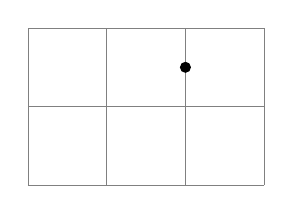
\begin{tikzpicture}
\draw[help lines] (0,0) grid (3,2);
\fill (canvas cs:x=2cm,y=1.5cm) circle (2pt);
\end{tikzpicture}
&
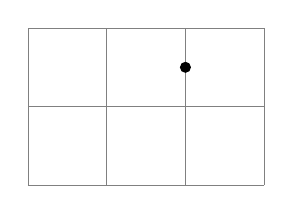
\begin{tikzpicture}
\draw[help lines] (0,0) grid (3,2);
\fill (2,1.5) circle (2pt);
\end{tikzpicture}

\\ \hline  
 \BS{fill} (\RDD{canvas cs}:\blll{x=2cm,y=1.5cm}) circle (2pt);
& \BS{fill} {\color{blue}(2cm,1.5cm)} circle (2pt);
\\ \hline 
\end{tabular} 


\SbSbSSCT{Système de coordonnées polaire \og canvas \fg}{Polar coordinates}

\noindent


\begin{tabular}{|c|c|c|} \hline
\TFRGB{Explicite}{explicit}  & \TFRGB{Implicite}{implicit}
\\ \hline
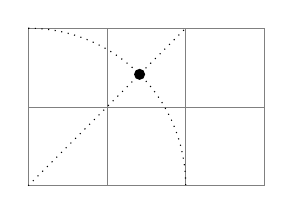
\begin{tikzpicture}
\draw[help lines] (0,0) grid (3,2);
\draw [dotted](0,2) arc (90 :0 :2);
\draw [dotted](0,0) --(2,2);
\fill (canvas polar cs:angle=45,radius=2cm) circle (2pt);
\end{tikzpicture}
&
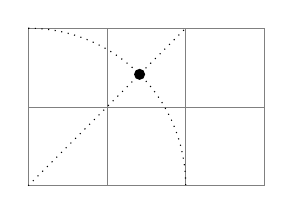
\begin{tikzpicture}
\draw[help lines] (0,0) grid (3,2);
\draw [dotted](0,2) arc (90 :0 :2);
\draw [dotted](0,0) --(2,2);
\fill (45:2cm) circle (2pt);
\end{tikzpicture}
\\ \hline 
\BS{fill} (\RDD{canvas polar cs}:\RDD{angle}=45,\RDD{radius}=2cm) circle (2pt);
&
\BS{fill} {\color{blue}(45:2cm)} circle (2pt);
\\ \hline 
\end{tabular} 

\bigskip
\begin{tabular}{|c|} \hline  
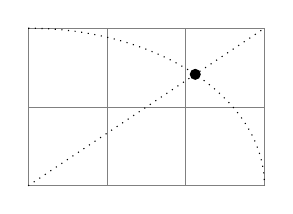
\begin{tikzpicture}
\draw[help lines] (0,0) grid (3,2);
\draw [dotted](0,2) arc (90 :0 :3 and 2);
\draw [dotted](0,0) --(3,2);
\fill (canvas polar cs:angle=45,x radius=3cm,y radius=2cm) circle (2pt);
\end{tikzpicture}
\\ \hline  
\BS{fill} (canvas polar cs:angle=45,\RDD{x radius}=3cm,\RDD{y radius}=2cm) circle (2pt);
\\ \hline 
\end{tabular}


\SbSbSSCT{Système de coordonnées  xyz}{xyz coordinates}

\noindent


\begin{tabular}{|c|c|c|} \hline 
\begin{tikzpicture}[->]
\draw (0,0) -- (xyz cs:x=1);
\draw[red] (0,0) -- (xyz cs:y=1);
\draw[magenta] (0,0) -- (xyz cs:z=1);
\end{tikzpicture}
&
\begin{tikzpicture}[->]
\draw (0,0) -- (1,0,0);
\draw[red]  (0,0) -- (0,1,0);
\draw[magenta]  (0,0) -- (0,0,1);
\end{tikzpicture}
\\ \hline 
\BS{draw} (0,0) - - (\RDD{xyz cs}:x=1); & \BS{draw}  (0,0) - - (1,0,0); \\
\BS{draw}[red]  (0,0) - - (\RDD{xyz cs}:y=1); &  \BS{draw}[red] (0,0) - - (0,1,0); \\
\BS{draw}[magenta]  (0,0) - - (\RDD{xyz cs}:z=1); &  \BS{draw}[magenta]   (0,0) - - (0,0,1); 
\\ \hline 

\end{tabular} 

 
\newpage

\SbSbSSCT{Coordinate system xyz polar}{Coordinate system xyz polar}

\noindent

\begin{tabular}{|c|c|c|} \hline
\TFRGB{Explicite}{explicit}  & \TFRGB{Implicite}{implicit}
\\ \hline
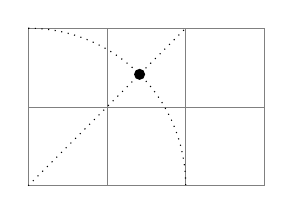
\begin{tikzpicture}
\draw[help lines] (0,0) grid (3,2);
\draw [dotted](0,2) arc (90 :0 :2);
\draw [dotted](0,0) --(2,2);
\fill (xyz polar cs:angle=45,radius=2) circle (2pt);
\end{tikzpicture}
&
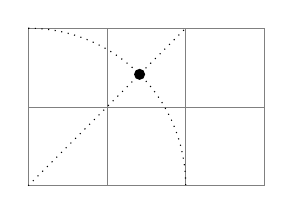
\begin{tikzpicture}
\draw[help lines] (0,0) grid (3,2);
\draw [dotted](0,2) arc (90 :0 :2);
\draw [dotted](0,0) --(2,2);
\fill (45:2) circle (2pt);
\end{tikzpicture}
\\ \hline 
\BS{fill} (\RDD{xyz polar cs}:\RDD{angle}=45,\RDD{radius}=2) circle (2pt);
&
\BS{fill} {\color{blue}(45:2cm)} circle (2pt);
\\ \hline 
\end{tabular} 

\bigskip
\begin{tabular}{|c|} \hline  
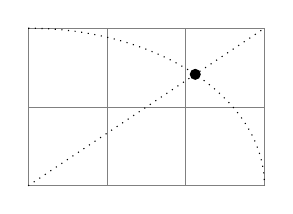
\begin{tikzpicture}
\draw[help lines] (0,0) grid (3,2);
\draw [dotted](0,2) arc (90 :0 :3 and 2);
\draw [dotted](0,0) --(3,2);
\fill (xyz polar cs:angle=45,x radius=3,y radius=2) circle (2pt);
\end{tikzpicture}
\\ \hline  
\BS{fill} (xyz polar cs:angle=45,\RDD{x radius}=3,\RDD{y radius}=2) circle (2pt);
\\ \hline 
\end{tabular} 

\bigskip

\begin{tabular}{|c|c|c|} \hline
\multicolumn{2}{|c|}{\BS{begin}\AC{tikzpicture}{\color{red}[x=1.5cm,y=1cm]} }
\\ \hline
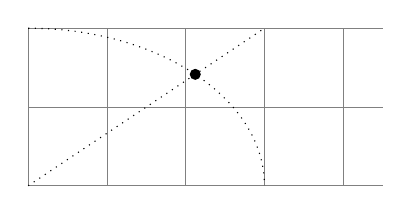
\begin{tikzpicture}[x=1.5cm,y=1cm]
\draw[help lines] (0,0) grid (3,2);
\draw [dotted](0,2) arc (90 :0 :2);
\draw [dotted](0,0) --(2,2);
\fill (xyz polar cs:angle=45,radius=2) circle (2pt);
\end{tikzpicture}
&
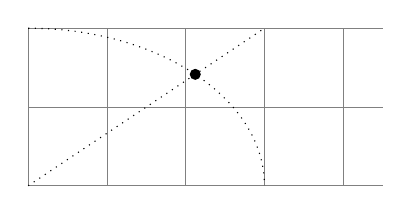
\begin{tikzpicture}[x=1.5cm,y=1cm]
\draw[help lines] (0,0) grid (3,2);
\draw [dotted](0,2) arc (90 :0 :2);
\draw [dotted](0,0) --(2,2);
\fill (45:2) circle (2pt);
\end{tikzpicture}
\\ \hline 
\BS{fill} (\RDD{xyz polar cs}:\RDD{angle}=45,\RDD{radius}=2) circle (2pt);
&
\BS{fill} {\color{blue}(45:2cm)} circle (2pt);
\\ \hline 
\end{tabular} 
\bigskip

\begin{tabular}{|c|c|c|} \hline
\multicolumn{2}{|c|}{\BS{begin}\AC{tikzpicture}{\color{red}[x=\AC{(0cm,1cm)},y=\AC{(-1cm,0cm)}]} }
\\ \hline
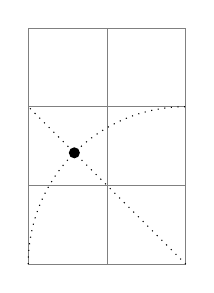
\begin{tikzpicture}[x={(0cm,1cm)},y={(-1cm,0cm)}]
\draw[help lines] (0,0) grid (3,2);
\draw [dotted](0,2) arc (90 :0 :2);
\draw [dotted](0,0) --(2,2);
\fill (xyz polar cs:angle=45,radius=2) circle (2pt);
\end{tikzpicture}
&
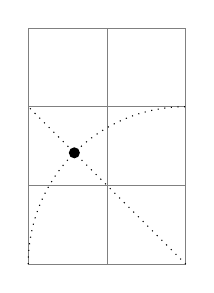
\begin{tikzpicture}[x={(0cm,1cm)},y={(-1cm,0cm)}]
\draw[help lines] (0,0) grid (3,2);
\draw [dotted](0,2) arc (90 :0 :2);
\draw [dotted](0,0) --(2,2);
\fill (45:2) circle (2pt);
\end{tikzpicture}
\\ \hline 
\BS{fill} (\RDD{xyz polar cs}:\RDD{angle}=45,\RDD{radius}=2) circle (2pt);
&
\BS{fill} {\color{blue}(45:2cm)} circle (2pt);
\\ \hline 
\end{tabular} 

\SbSbSSCT{Coordonnées barycentriques}{Barycentric coordinates}

\begin{center}
\RRR{13-2-2}
\end{center}

\begin{tabular}{|c|c|c|} \hline
\multicolumn{3}{|c|}{  \BS{node} [circle,fill=red!20] at (\RDD{barycentric cs}:A=0.6,B=0.3 ) \AC{X};   }\\ 
\hline
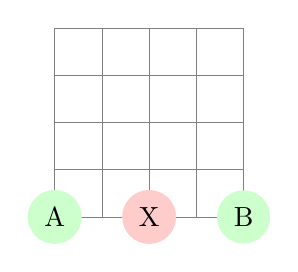
\begin{tikzpicture}[scale=.6]
\draw[help lines] (0,0) grid (4,4);
\node[circle,fill=green!20,] (A) at (0,0) {A};
\node[circle,fill=green!20,] (B) at (4,0) {B};
\node[circle,fill=red!20] at (barycentric cs:A=0.3,B=0.3 ) {X};
\end{tikzpicture}
&
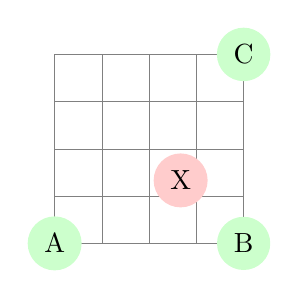
\begin{tikzpicture}[scale=.6]
\draw[help lines] (0,0) grid (4,4);
\node[circle,fill=green!20,] (A) at (0,0) {A};
\node[circle,fill=green!20,] (B) at (4,0) {B};
\node[circle,fill=green!20,] (C) at (4,4) {C};
\node[circle,fill=red!20] at (barycentric cs:A=0.4,B=0.4 ,C=.4) {X};
\end{tikzpicture}
&
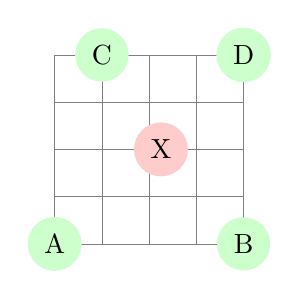
\begin{tikzpicture}[scale=.6]
\draw[help lines] (0,0) grid (4,4);
\node[circle,fill=green!20,] (A) at (0,0) {A};
\node[circle,fill=green!20,] (B) at (4,0) {B};
\node[circle,fill=green!20,] (C) at (1,4) {C};
\node[circle,fill=green!20,] (D) at (4,4) {D};
\node[circle,fill=red!20] at (barycentric cs:A=0.5,B=0.5,C=.5,D=.5 ) {X};
\end{tikzpicture}
\\ \hline
A=0.3,B=0.3 & A=0.4,B=0.4 ,C=.4 & A=0.5,B=0.5,C=.5,D=.5 
\\ \hline
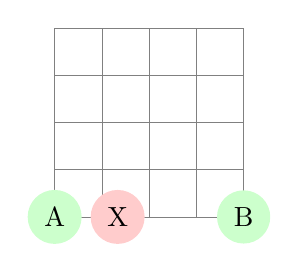
\begin{tikzpicture}[scale=.6]
\draw[help lines] (0,0) grid (4,4);
\node[circle,fill=green!20,] (A) at (0,0) {A};
\node[circle,fill=green!20,] (B) at (4,0) {B};
\node[circle,fill=red!20] at (barycentric cs:A=0.6,B=0.3 ) {X};
\end{tikzpicture}
&
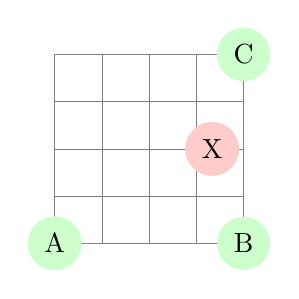
\begin{tikzpicture}[scale=.6]
\draw[help lines] (0,0) grid (4,4);
\node[circle,fill=green!20,] (A) at (0,0) {A};
\node[circle,fill=green!20,] (B) at (4,0) {B};
\node[circle,fill=green!20,] (C) at (4,4) {C};
\node[circle,fill=red!20] at (barycentric cs:A=0.2,B=0.4 ,C=.6) {X};
\end{tikzpicture}
&
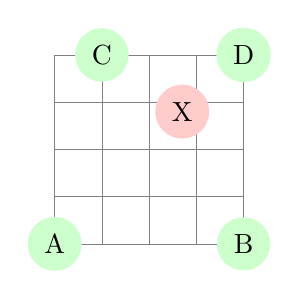
\begin{tikzpicture}[scale=.6]
\draw[help lines] (0,0) grid (4,4);
\node[circle,fill=green!20,] (A) at (0,0) {A};
\node[circle,fill=green!20,] (B) at (4,0) {B};
\node[circle,fill=green!20,] (C) at (1,4) {C};
\node[circle,fill=green!20,] (D) at (4,4) {D};
\node[circle,fill=red!20] at (barycentric cs:A=0.2,B=0.4,C=.6,D=.8 ) {X};
\end{tikzpicture}
\\ \hline
A=0.6,B=0.3 & A=0.2,B=0.4 ,C=.6 & A=0.2,B=0.4,C=.6,D=.8
\\ \hline
\end{tabular}

\SbSbSSCT{Coordonnées nominatives : n\oe ud}{Named coordinates: nodes}

\begin{center}
\RRR{13-2-3}
\end{center}

\begin{tabular}{|c|c|} \hline  
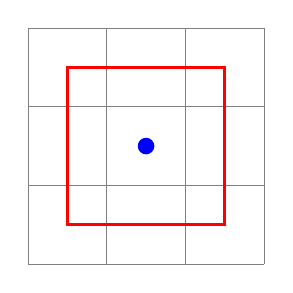
\begin{tikzpicture}[blue,very thick,baseline=1cm]
\draw[help lines] (0,0) grid (3,3);
\coordinate (centre) at (1.5,1.5) ;
\coordinate (A) at (.5,.5) ;
\coordinate (B) at (2.5,2.5) ;
\fill (centre) circle (3pt);
\draw[red] (A) rectangle (B) ;
\end{tikzpicture}
&  
\parbox[c]{8cm}{
\BSS{coordinate} {\color{blue}(centre)} at(1.5,1.5) ; \\
\BSS{coordinate} {\color{blue}(A)} at (.5,.5) ;\\
\BSS{coordinate} {\color{blue}(B)} at  (2.5,2.5) ;\\
\\
\BS{fill} {\color{blue}(centre)} circle (3pt);\\
\BS{draw}[red] {\color{blue}(A)} rectangle {\color{blue}(B)} ;\\
}
\\ \hline 
\end{tabular} 


\TFRGB{voir aussi}{see also} page \pageref{noeuds}


\SbSbSSCT{Coordonnées relatives à un noeud}{Coordinates relative to a node}

\noindent

\begin{tabular}{|c|c|c|c|} \hline
\multicolumn{4}{|l|}{  \BS{node} [draw,fill=green!20,] (A) at (1,1) \AC{\BS{huge}  noeud}; }\\ 
\multicolumn{4}{|l|}{  \BS{fill}[red] (\RDD{node cs}:\RDD{name}=A,\RDD{anchor}=south) circle (3pt);   }\\ 
\hline

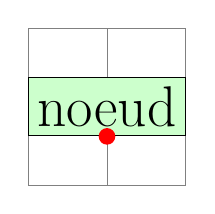
\begin{tikzpicture}
\draw[help lines] (0,0) grid (2,2);
\node[draw,fill=green!20,] (A) at (1,1) {\huge noeud};
\fill[red] (node cs:name=A,anchor=south) circle (3pt);
\end{tikzpicture}
&
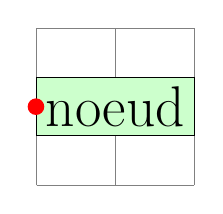
\begin{tikzpicture}
\draw[help lines] (0,0) grid (2,2);
\node[draw,fill=green!20,] (A) at (1,1) {\huge noeud};
\fill[red] (node cs:name=A,anchor=west) circle (3pt);
\end{tikzpicture}
&
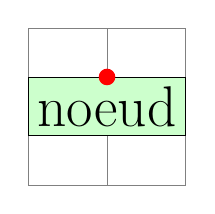
\begin{tikzpicture}
\draw[help lines] (0,0) grid (2,2);
\node[draw,fill=green!20,] (A) at (1,1) {\huge noeud};
\fill[red] (node cs:name=A,anchor=north) circle (3pt);
\end{tikzpicture}
&
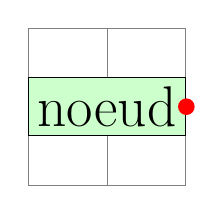
\begin{tikzpicture}
\draw[help lines] (0,0) grid (2,2);
\node[draw,fill=green!20,] (A) at (1,1) {\huge noeud};
\fill[red] (node cs:name=A,anchor=east) circle (3pt);
\end{tikzpicture}
\\ \hline
name=A,anchor=south & name=A,anchor=west & name=A,anchor=north & name=A,anchor=east
\\ \hline
\end{tabular}

\bigskip

\begin{tabular}{|c|c|c|c|} \hline
\multicolumn{4}{|l|}{  \BS{node} [draw,fill=green!20,] \blll{(A)} at (1,1) \AC{\BS{huge}  noeud}; }\\ 
\multicolumn{4}{|l|}{  \BS{fill}[red] (\blll{A}.south) circle (3pt);   }\\ 
\hline

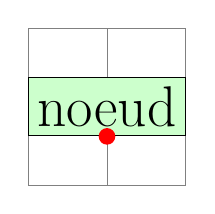
\begin{tikzpicture}
\draw[help lines] (0,0) grid (2,2);
\node[draw,fill=green!20,] (A) at (1,1) {\huge noeud};
\fill[red] (A.south) circle (3pt);
\end{tikzpicture}
&
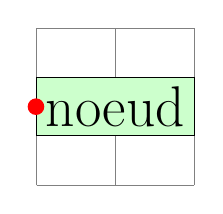
\begin{tikzpicture}
\draw[help lines] (0,0) grid (2,2);
\node[draw,fill=green!20,] (A) at (1,1) {\huge noeud};
\fill[red] (A.west) circle (3pt);
\end{tikzpicture}
&
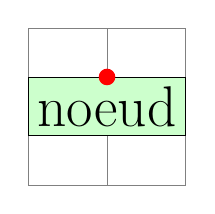
\begin{tikzpicture}
\draw[help lines] (0,0) grid (2,2);
\node[draw,fill=green!20,] (A) at (1,1) {\huge noeud};
\fill[red] (A.north) circle (3pt);
\end{tikzpicture}
&
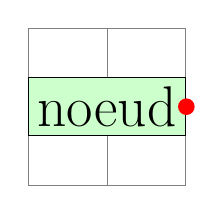
\begin{tikzpicture}
\draw[help lines] (0,0) grid (2,2);
\node[draw,fill=green!20,] (A) at (1,1) {\huge noeud};
\fill[red] (A.east) circle (3pt);
\end{tikzpicture}
\\ \hline
A.south & A.west & A.north & A.east
\\ \hline
\end{tabular}



\bigskip
\begin{tabular}{|c|c|c|c|} \hline
\multicolumn{4}{|c|}{  \BS{fill}[red] (node cs:\RDD{name}=A,\RDD{angle}=0) circle (3pt);  }\\ 
\hline

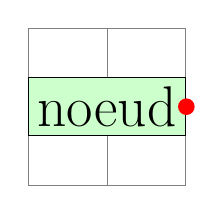
\begin{tikzpicture}
\draw[help lines] (0,0) grid (2,2);
\node[draw,fill=green!20,] (A) at (1,1) {\huge noeud};
\fill[red] (node cs:name=A,angle=0) circle (3pt);
\end{tikzpicture}
&
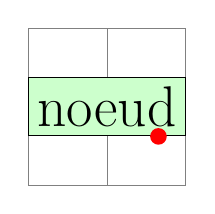
\begin{tikzpicture}
\draw[help lines] (0,0) grid (2,2);
\node[draw,fill=green!20,] (A) at (1,1) {\huge noeud};
\fill[red] (node cs:name=A,angle=-30) circle (3pt);
\end{tikzpicture}
&
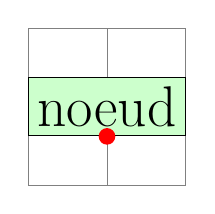
\begin{tikzpicture}
\draw[help lines] (0,0) grid (2,2);
\node[draw,fill=green!20,] (A) at (1,1) {\huge noeud};
\fill[red] (node cs:name=A,angle=-90) circle (3pt);
\end{tikzpicture}
&
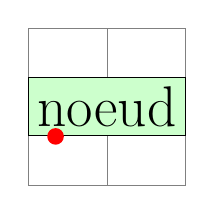
\begin{tikzpicture}
\draw[help lines] (0,0) grid (2,2);
\node[draw,fill=green!20,] (A) at (1,1) {\huge noeud};
\fill[red] (node cs:name=A,angle=-150) circle (3pt);
\end{tikzpicture}
\\ \hline
name=A,angle=0 & name=A,angle=-30 & nname=A,angle=-90 & name=A,angle=-150
\\ \hline
\end{tabular}

\bigskip


\begin{tabular}{|c|c|c|c|} \hline
\multicolumn{4}{|c|}{  \BS{fill}[red] (A.0) circle (3pt);  }\\ 
\hline

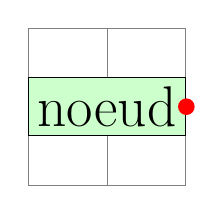
\begin{tikzpicture}
\draw[help lines] (0,0) grid (2,2);
\node[draw,fill=green!20,] (A) at (1,1) {\huge noeud};
\fill[red] (A.0) circle (3pt);
\end{tikzpicture}
&
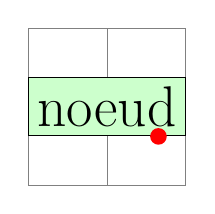
\begin{tikzpicture}
\draw[help lines] (0,0) grid (2,2);
\node[draw,fill=green!20,] (A) at (1,1) {\huge noeud};
\fill[red] (A.-30) circle (3pt);
\end{tikzpicture}
&
\begin{tikzpicture}
\draw[help lines] (0,0) grid (2,2);
\node[draw,fill=green!20,] (A) at (1,1) {\huge noeud};
\fill[red] (A.-90) circle (3pt);
\end{tikzpicture}
&
\begin{tikzpicture}
\draw[help lines] (0,0) grid (2,2);
\node[draw,fill=green!20,] (A) at (1,1) {\huge noeud};
\fill[red] (A.-150) circle (3pt);
\end{tikzpicture}
\\ \hline
A.0 & A.-30 & A.-90 & A.-150
\\ \hline
\end{tabular}

\TFRGB{voir aussi}{see also} page \pageref{nomnoeud}


\newpage

\SbSbSSCT{Coordonnées relatives à deux points}{Coordinates relative to two points}
\begin{center}
\RRR{13-3-1}
\end{center}

\begin{tabular}{|c|c|} \hline
\multicolumn{2}{|c|}{  \BS{node} [circle,fill=red!20] at (1,1 {\color{red}|-} 3,3) \AC{X}   }\\ 
\hline
\begin{tikzpicture}
\draw[help lines] (0,0) grid (4,4);
\node[circle,fill=green!20,] (A) at (1,1) {A};
\node[circle,fill=green!20,] (B) at (3,3) {B};
\node[circle,fill=red!20] at (1,1 |- 3,3) {X};
\end{tikzpicture}
&
\begin{tikzpicture}
\draw[help lines] (0,0) grid (4,4);
\node[circle,fill=green!20,] (A) at (1,1) {A};
\node[circle,fill=green!20,] (B) at (3,3) {B};
\node[circle,fill=red!20] at (1,1 -| 3,3) {X};
\end{tikzpicture}
\\ \hline
at (1,1 {\color{red}|-} 3,3)
&
at (1,1 {\color{red}-|} 3,3)
\\ \hline
\end{tabular}



\SbSbSSCT{Coordonnée relative à une intersection}{Coordinates relative to an intersection}
\begin{center}
\RRR{13-3-2}
\end{center}

 \maboite{\BS{usetikzlibrary}\AC{intersections}}
\label{lib-intersections}


\begin{tabular}{|c|c|c|c|} \hline 
\multicolumn{4}{|l|}{  \BS{draw} [\RDD{name path}=XXX] (2,1) circle  (1cm);   }\\ 
\multicolumn{4}{|l|}{  \BS{draw} [\RDD{name path}=YYY] (0.5,0.5) rectangle +(3,1);   }\\ 
\multicolumn{4}{|l|}{ \BS{fill} [red,\RDD{ name intersections}=\AC{of=xxx and YYY}]
(\RDD{intersection}-1) circle (2pt)   }\\ 
\hline 
\begin{tikzpicture}[scale=.8]
\draw [help lines] grid (4,2);
\draw [name path=XXX] (2,1) circle  (1cm);
\draw [name path=YYY] (0.5,0.5) rectangle +(3,1);
\fill [red, name intersections={of=XXX and YYY}]
(intersection-1) circle (2pt)  ;
\end{tikzpicture}
& 
\begin{tikzpicture}[scale=.8]
\draw [help lines] grid (4,2);
\draw [name path=XXX] (2,1) circle  (1cm);
\draw [name path=YYY] (0.5,0.5) rectangle +(3,1);
\fill [red, name intersections={of=XXX and YYY}] (intersection-2) circle (2pt) ;
\end{tikzpicture} 
&  
\begin{tikzpicture}[scale=.8]
\draw [help lines] grid (4,2);
\draw [name path=XXX] (2,1) circle  (1cm);
\draw [name path=YYY] (0.5,0.5) rectangle +(3,1);
\fill [red, name intersections={of=XXX and YYY}] (intersection-3) circle (2pt) ;
\end{tikzpicture}
&  
\begin{tikzpicture}[scale=.8]
\draw [help lines] grid (4,2);
\draw [name path=XXX] (2,1) circle  (1cm);
\draw [name path=YYY] (0.5,0.5) rectangle +(3,1);
\fill [red, name intersections={of=XXX and YYY}] (intersection-4) circle (2pt) ;
\end{tikzpicture}
\\ 
\hline intersection-1 & intersection-2 &intersection-3  & intersection-4 \\ 
\hline 
\end{tabular} 

\bigskip

\begin{tabular}{|c|} \hline  
\BS{fill} [red, name intersections=\AC{of=XXX and YYY}] \\
(intersection-1) circle (2pt) {\color{red} node[black,above right] \AC{point a}} ;
\\ \hline  
\begin{tikzpicture}
\draw [help lines] grid (4,2);
\draw [name path=XXX] (2,1) circle  (1cm);
\draw [name path=YYY] (0.5,0.5) rectangle +(3,1);
\fill [red, name intersections={of=XXX and YYY}]
(intersection-1) circle (2pt) node[black,above right] {point a} ;
\end{tikzpicture} 
\\ \hline 
\end{tabular} 

\bigskip

\begin{tabular}{|c|} \hline 
\BS{fill} [red, name intersections=\AC{of=XXX and YYY, \RDD{name}=ZZZ}]; \\
\BS{draw} [red] (ZZZ-1) - - (ZZZ-3); \BS{draw} [green] (ZZZ-2) - - (ZZZ-4);
\\ \hline  
\begin{tikzpicture}
\draw [help lines] grid (4,2);
\draw [name path=XXX] (2,1) circle  (1cm);
\draw [name path=YYY] (0.5,0.5) rectangle +(3,1);
\fill [red, name intersections={of=XXX and YYY, name=ZZZ}];
\draw [red] (ZZZ-1) -- (ZZZ-3);
\draw [green] (ZZZ-2) -- (ZZZ-4);
\end{tikzpicture}
\\ \hline 
\end{tabular} 

\bigskip
\begin{tabular}{|c|} \hline  
\BS{fill} [red, name intersections=\AC{of=XXX and YYY , \RDD{by}=\AC{a,b,c,d}}]; \\
\BS{draw} [red] (a) - - (c); \hspace{1cm} \BS{draw} [green] (b) - - (d);
\\ \hline   
\begin{tikzpicture}
\draw [help lines] grid (4,2);
\draw [name path=XXX] (2,1) circle  (1cm);
\draw [name path=YYY] (0.5,0.5) rectangle +(3,1);
\fill [red, name intersections={of=XXX and YYY, by={a,b,c,d}}];
\draw [red] (a) -- (c);
\draw [green] (b) -- (d);
\end{tikzpicture}
\\ \hline 
\end{tabular} 

\bigskip

\begin{tabular}{|c|} \hline  
\BS{fill} [name intersections=\AC{of=XXX and YYY, name=i, \RDD{total}=\BS{t}}] [red] \\
\BS{foreach} \BS{s} in \AC{1,...,\BS{t}} \AC{(i-\BS{s}) circle (2pt) node[black,above right] \AC{\BS{s}}}
\\ \hline  
\begin{tikzpicture}
\draw [help lines] grid (4,2);
\draw [name path=XXX] (2,1) circle  (1cm);
\draw [name path=YYY] (0.5,0.5) rectangle +(3,1);
\fill [name intersections={of=XXX and YYY , name=i, total=\t}]
[red]
\foreach \s in {1,...,\t}{(i-\s) circle (2pt) node[black,above right] {\s}};
\end{tikzpicture}
\\ \hline 
\end{tabular} 



\newpage

\SbSbSSCT{Position calculée avec le module  \og  pgfmath \fg}{Calculated positions with  \og  pgfmath \fg }

\begin{center}
\RRR{13-2-1}
\end{center}

\TFRGB{Ce module est chargé automatiquement avec le module Tikz}{Package automatically loaded with Tikz} 

\begin{tabular}{|c|} \hline 
\begin{tikzpicture}
\draw[help lines] (0,0) grid (4,2);
\fill [red] (canvas cs:x=2cm+1.5cm,y=1.5cm-1cm) circle (3pt);
\fill [blue] (2cm,1.5cm) circle (3pt);
\draw[dashed] (2,1.5) -| (3.5,.5);
\end{tikzpicture}
\\ \hline 
\emph{\TFRGB{Explicite}{explicit}} 
 : \BS{fill} [red] (\RDD{canvas cs}:x=2cm+1.5cm,y=1.5cm-1cm) circle (3pt);
 \\  \hline 
\emph{\TFRGB{Implicite}{implicit}} :  \BS{fill} [red] {\color{red}(2cm+1.5cm,1.5cm-1cm)} circle (3pt);
\\ \hline 
\end{tabular} 

\bigskip
\begin{tabular}{|c|c|c|} \hline 
\begin{tikzpicture}[baseline=0pt]
\draw[help lines] (0,0) grid (4,4);
 \draw[dashed] (2,2) circle (2);
\fill[red](2+ 2*cos 30,2+2*sin 30) circle (3pt);
\fill[magenta](2+ 2*cos{(120)},2+2*sin{(120)}) circle (3pt);
\end{tikzpicture}
&
\parbox[c]{8cm}{
 \BS{draw}[dashed] (2,2) circle (2);\\
 \smallskip
 \BS{fill} [red]{\color{red}(2+ 2*cos 30 , 2+2*sin 30)} circle (3pt);\\
  \smallskip
 \BS{fill}[magenta] {\color{red}(2+2*cos\AC{(120)} , 2+2*sin\AC{(120)})} circle (3pt); 
 }
\\ \hline 
\end{tabular} 

\SbSbSSCT{Position calculée avec \og library calc \fg}{Calculated positions with \og  calc  library calc \fg}

\begin{center}
\RRR{13-5}
\end{center}
\label{lib-calc}

 \maboite{\BS{usetikzlibrary}\AC{calc}}
 
\begin{tabular}{|c|c|} \hline  
\begin{tikzpicture}[baseline=0pt]
\draw [help lines] (0,0) grid (3,2);
\node (a) at (1,1) {A};
\fill [red] ($(a) + 2/3*(1cm,0)$) circle (2pt);
\fill [red] ($(a) + 4/3*(1cm,0)$) circle (2pt);
\end{tikzpicture}
&
\parbox{8cm}{
\BS{node} (a) at (1,1) \AC{A}; \\
\BS{fill} [red] {\color{red} (\$(a) + 2/3*(1cm,0)\$)} circle (2pt); \\
\BS{fill} [red] {\color{red}(\$(a) + 4/3*(1cm,0)\$)} circle (2pt); \\
}
\\ 
\hline 
\end{tabular} 

\SbSbSSCT{Tangentes avec \og library calc \fg}{Tangents with  \og calc library  \fg}

\begin{center}
\RRR{13-2-4}
\end{center}

\begin{tabular}{|c|c|} \hline 
\multicolumn{2}{|l|}{\BS{node}[fill=green!20] (a) at (3,1.5) \AC{A}; } \\
\multicolumn{2}{|l|}{\BS{fill}[red] (\RDD{tangent cs}:\RDD{node}=c,\RDD{point}=\AC{(A)},\RDD{solution}=1);  }\\ 
\hline
\begin{tikzpicture}
\draw[help lines] (0,0) grid (4,2);
\node[fill=green!20] (A) at (3,1.5) {A};
\node [circle,draw] (c) at (1,1) [minimum size=1.5cm] {$c$};
\draw[red,dashed] (A) - -(tangent cs:node=c,point={(A)},solution=1) ;
\draw[red,dashed] (1,1) - -(tangent cs:node=c,point={(3,1.5)},solution=1) ;
\fill[red] (tangent cs:node=c,point={(A)},solution=1) circle (3pt);
\end{tikzpicture}
&
\begin{tikzpicture}
\draw[help lines] (0,0) grid (4,2);
\node[fill=green!20] (A) at (3,1.5) {A};
\node [circle,draw] (c) at (1,1) [minimum size=1.5cm] {$c$};
\draw[red,dashed] (A) - -(tangent cs:node=c,point={(A)},solution=2) ;
\draw[red,dashed] (1,1) - -(tangent cs:node=c,point={(A)},solution=2) ;
\fill[red] (tangent cs:node=c,point={(A)},solution=2) circle (3pt);
\end{tikzpicture}
\\ \hline
\RDD{solution}=1 & \RDD{solution}=2
\\ \hline
\end{tabular} 

\newpage

\SbSbSSCT{Point à pourcentage donné }{Percentage position }

\begin{center}
\RRR{13-5-3}
\end{center}


\begin{tabular}{|c|c|} \hline  
\multicolumn{2}{|c|}{\BS{fill}[red] ({\color{red}\$(0,1)!.25!(4,1)\$}) circle (4pt); } \\  \hline  

\begin{tikzpicture}
\draw [help lines] (0,0) grid (4,2);
\draw [line width= 3pt] (0,1) -- (4,1);
\fill[red] ($(0,1)!.25!(4,1)$) circle (4pt);
\end{tikzpicture}
&  
\begin{tikzpicture}
\draw [help lines] (0,0) grid (4,2);
\draw [line width= 3pt] (0,1) -- (4,1);
\fill[red] ($(0,1)!.75!(4,1)$) circle (4pt);
\end{tikzpicture}
\\ \hline (0,1)!{\color{red}0.25}!(4,1) & (0,1)!{\color{red}0.75}!(4,1) \\ 
\hline 
\end{tabular} 

\bigskip

\begin{tabular}{|c|} \hline  
\begin{tikzpicture}
\draw [help lines] (0,0) grid (4,3);
\draw [line width=2pt ](0,2) -- (4,2);
\draw[red] ($(0,2)!.75!(4,2)$) -- (0,0);
\fill[red] ($(0,2)!.75!(4,2)!.66!(0,0)$) circle (4pt);
\end{tikzpicture}
\\ \hline 
\BS{fill}[red] (\${\color{blue}(0,2)!0.75!(4,2)}!{\color{red}0.66!(0,0)}\$) circle (2pt);
\\ \hline 
\end{tabular} 


\SbSbSSCT{Point à distance donnée}{Position at a given distance }

\begin{center}
\RRR{13-5-4}
\end{center}

\begin{tabular}{|c|c|} \hline  
\multicolumn{2}{|c|}{\BS{fill}[red] ({\color{red}\$(0,1)!1.5cm!(4,1)\$}) circle (4pt); } \\  \hline  

\begin{tikzpicture}
\draw [help lines] (0,0) grid (4,2);
\draw [line width= 2pt] (0,1) -- (4,1);
\fill[red] ($(0,1)!1.5cm!(4,1)$) circle (4pt);
\end{tikzpicture}
&  
\begin{tikzpicture}
\draw [help lines] (0,0) grid (4,2);
\draw [line width= 2pt] (0,1) -- (4,1);
\fill[red] ($(0,1)!3cm!(4,1)$) circle (4pt);
\end{tikzpicture}
\\ \hline (0,1)!{\color{red}1.5cm}!(4,1) & (0,1)!{\color{red}3cm}!(4,1) \\ 
\hline 
\end{tabular} 

\bigskip

\begin{tabular}{|c|} \hline  
\begin{tikzpicture}
\draw [help lines] (0,0) grid (4,4);
\coordinate (a) at (1,0);
\coordinate (b) at (4,1);
\draw [line width= 3pt] (0,0) -- (4,1);
\draw [line width= 2pt,red](2,.5) -- ($ (2,.5)!2cm!90:(4,1) $);
\end{tikzpicture}
\\ \hline
\BS{draw} (2,.05) - - (\$ (2,0.5)!{\color{red}2cm!90:(4,1)} \$);
\\ \hline 
\end{tabular} 

\newpage

\SbSbSSCT{Coordonnées relatives}{Relative coordinates}


\Par{Cartésienne}{Cartesian coordinates}

\begin{center}
\RRR{13-4-1}
\end{center}

\begin{tabular}{|c|c|c|} \hline  
\TFRGB{relative à l'origine}{relative to the origin}  & \TFRGB{relative à une position}{relative to a position}  &  \TFRGB{relative à la dernière position}{relative to the last position}   
\\ \hline  
 
\begin{tikzpicture}
\draw[help lines] (0,-1) grid (3,1); 
 \draw[blue,very thick] (0,0) -- (1,0) - - (2,1) - - (2,-1);
 \fill[red] (0,0) circle (4pt);
\end{tikzpicture}
&
\begin{tikzpicture} %[scale=.8]
\draw[help lines] (0,-1) grid (4,1);
 \draw[blue,very thick] (0,0) - - (1,0) -- +(2,1) -- +(2,-1) ; %–- +(2,-1) ;
 \fill[red] (1,0) circle (4pt);
\end{tikzpicture}
&
\begin{tikzpicture} %[scale=.8]
\draw[help lines] (0,-1) grid (5,1);  
 \draw[blue,very thick] (0,0) -- (1,0)  - - ++(2,1) - - ++(2,-1);
 \fill[red] (1,0) circle (4pt);
 \fill[red] (3,1) circle (4pt);
\end{tikzpicture}
\\ \hline 
\tikz \fill node[fill=green!20,inner sep=0pt]{(0,0)}; - - (1,0) &
 (0,0) - - \tikz \fill node[fill=green!20,inner sep=0pt]{(1,0)};  & (0,0) - - \tikz \fill node[fill=green!20,inner sep=0pt]{(1,0)}; \\
 - - (2,1) - - (2,-1)  &
   - - +(2,1) - - +(2,-1) & - - ++\tikz \fill node[fill=green!20,inner sep=0pt]{(2,1)}; - - ++(2,-1)
\\ \hline 
\end{tabular} 

\bigskip

\begin{tabular}{|c|c|c|} \hline  
\begin{tikzpicture} [scale=.5]
\draw[help lines] (0,-1) grid (6,6);
 \draw[red,dotted,line width=2pt] (0,0) rectangle (2,2) ;
  \draw[green,dotted,line width=2pt] (0,0) rectangle (3,3) ;  
 \draw[blue,line width=2pt] (0,0) rectangle (1,1)  rectangle (2,2) rectangle (3,3);

\end{tikzpicture}

&  
\begin{tikzpicture} [scale=.5]
\draw[help lines] (0,-1) grid (6,6); 
  \draw[green,dotted,line width=2pt] (1,1) rectangle (4,4) ;   
 \draw[blue,line width=2pt] (0,0) rectangle (1,1)  rectangle +(2,2) rectangle +(3,3);
    \fill[red] (1,1) circle (4pt);
\end{tikzpicture}
&  
\begin{tikzpicture} [scale=.5]
\draw[help lines] (0,-1) grid (6,6);  
 \draw[blue,line width=2pt] (0,0) rectangle (1,1)  rectangle ++(2,2) rectangle ++(3,3);
    \fill[red] (1,1) circle (4pt);
     \fill[green] (3,3) circle (4pt); 
\end{tikzpicture}
\\ 
\hline 
\BS{draw} (0,0) rectangle (1,1)   &
\BS{draw} (0,0) rectangle (1,1)   & 
\BS{draw} (0,0) rectangle (1,1)  \\
rectangle (2,2) rectangle (3,3);  &
rectangle +(2,2) rectangle +(3,3);  &
rectangle ++(2,2) rectangle ++(3,3); \\
\hline 
\end{tabular}


\Par{Polaire }{Polar} {}

\bigskip


\noindent

\begin{tabular}{|c|c|c|c|} \hline
\TFRGB{relative à l'origine}{relative to the origin}  & \TFRGB{relative à une position}{relative to a position}  &  \TFRGB{relative à la dernière position}{relative to the last position}   
\\ \hline    
\begin{tikzpicture} %[scale=.8] 
\draw[help lines] (0,-1) grid (3,1);
 \fill[red] (0:0) circle (4pt);
 \draw[blue,very thick] (0:0)-- (0:1) -- (30:2) -- (-30:2);
\end{tikzpicture}
&
\begin{tikzpicture} %[scale=.8] 
\draw[help lines] (0,-1) grid (4,1);
 \fill[red] (1,0) circle (4pt);
 \draw[blue,very thick] (0:0) -- (0:1) -- +(30:2) -- +(-30:2);
\end{tikzpicture}
&
\begin{tikzpicture} %[scale=.8] 
\draw[help lines] (0,-1) grid (5,1);
 \fill[red] (1,0) circle (4pt);
 \fill[red] (2.732,1) circle (4pt);
 \draw[blue,very thick] (0:0)-- (0:1) -- ++(30:2) -- ++(-30:2);
\end{tikzpicture}
\\ \hline
\tikz \fill node[fill=green!20,inner sep=0pt] {(0:0)}; - - (0:1)&
 (0:0) - - \tikz \fill node[fill=green!20,inner sep=0pt] {(0:1)}; & (0:0)- - \tikz \fill node[fill=green!20,inner sep=0pt] {(0:1)}; \\
 - - (30:2) - - (-30:2)  &  - -  +(30:2) - - +(-30:2) & - -  ++\tikz \fill node[fill=green!20,inner sep=0pt] {(30:2)}; - - ++(-30:2)
\\ \hline 
\end{tabular} 

%\subsubsection{coordonnée relative en polaire}
\Par{coordonnée relative en polaire}{Relative polar coordinate}

\begin{center}
\RRR{13-4-2}
\end{center}
\bigskip

\begin{tabular}{|c|c|} \hline 
\multicolumn{2}{|c|}{ \BS{draw}[blue,very thick] (0,0) -- (2,1) -- ([turn]-45:1cm);}
 \\ \hline
\begin{tikzpicture} %[scale=.8] 
\draw[help lines] (0,0) grid (4,2);
 \draw[dotted] (0,0) -- (4,2);
 \draw[blue,very thick] (0,0) -- (2,1) -- ([turn]-45:1cm);
\end{tikzpicture}
&  
\begin{tikzpicture} %[scale=.8] 
\draw[help lines] (0,0) grid (4,2);
 \draw[dotted] (0,0) -- (4,2);
 \draw[blue,very thick] (0,0) -- (2,1) -- ([turn]45:1cm);
\end{tikzpicture}
\\ \hline ([\RDD{turn}]-45:1cm) & ([\RDD{turn}]45:1cm) \\ 
\hline 
\end{tabular}

\bigskip

\begin{tabular}{|c|c|} \hline  
\begin{tikzpicture}  
\draw[help lines] (-1,0) grid (4,3);
\draw [line width=2pt] (4,0) arc (0 :120 :2)  -- ([turn]90:2cm) ;

\end{tikzpicture}
&  
\begin{tikzpicture} %[scale=.8] 
\draw[help lines] (0,0) grid (4,3);
\draw [line width=2pt]  (0,0) to [bend left] (2,2) --  ([turn]0:2cm);
\fill [red](2,2) circle (4pt);
\end{tikzpicture}
\\ \hline  
\BS{draw} (4,0) arc (0 :120 :2)  - - ([\RDD{turn}]90:2cm) ;
& \BS{draw}  (0,0) to [bend left] (2,2) - -  ([\RDD{turn}]0:2cm); \\

\hline 
\end{tabular} 


%\bigskip 
%
%
%\tikz [delta angle=30, radius=1cm]
%\draw (0,0) arc [start angle=0] -- ([turn]0:1cm)
%arc [start angle=30] -- ([turn]0:1cm)
%arc [start angle=60] -- ([turn]30:1cm);



\bigskip

\begin{tabular}{|c|c|c|} \hline  
\multicolumn{3}{|c|}{ \BS{draw}(1,2)
.. controls ([turn]0:2cm) .. ([turn]-90:2cm); }
\\ \hline
\begin{tikzpicture} %[scale=.8] 
\draw[help lines] (0,0) grid (4,4);
 \draw [line width=2pt] (1,2)
.. controls ([turn]0:2cm) .. ([turn]-90:2cm);
\end{tikzpicture}
&  
\begin{tikzpicture} %[scale=.8] 
\draw[help lines] (0,0) grid (4,4);
 \draw [line width=2pt] (1,2)
.. controls ([turn]30:2cm) .. ([turn]-90:2cm);
\end{tikzpicture}
&  
\begin{tikzpicture} %[scale=.8] 
\draw[help lines] (-2,0) grid (2,4);
 \draw [line width=2pt] (1,2)
.. controls ([turn]0:2cm) .. ([turn]90:2cm);

\end{tikzpicture}
\\ \hline ([turn]0:2cm) .. ([turn]-90:2cm) & ([turn]30:2cm) .. ([turn]-90:2cm) & ([turn]0:2cm) .. ([turn]90:2cm) \\ 
\hline 
\end{tabular} 


\tikzset{every picture/.style=blue,very thick,inner sep=.3333em}

%
%
%
%\newpage
%
%\SSCT{Les n\oe uds }{Nodes}
%
%\SbSSCT{Définition des  n\oe uds}{Creation of nodes}
\tikzset{blue}

\label{noeuds}
\noindent

\begin{tabular}{|c | c | c | c | c |} \hline
\multicolumn{5}{|c|}{  \BS{draw} (1,1) node[\RDD{fill}=red!20] \AC{};   }\\ 
\hline 
\tikz \draw (0,0) grid (2,2) (1,1) node[fill=red!20] {};
&
\tikz \draw (0,0) grid (2,2) (1,1) node[fill=red!20,draw] {}; 
&
\tikz \draw (0,0) grid (2,2) (1,1) node[circle,fill=red!20] {};
&
\tikz \draw (0,0) grid (2,2) (1,1) node[circle,fill=red!20,draw] {};
&
\tikz \draw (0,0) grid (2,2) (1,1) node[coordinate] {};
\\  \hline
\dft
&
node[\RDD{draw}] 
&
 node[\RDD{circle}]  
&
 node[\RDD{circle},\RDD{draw}]
 &
  node[\RDD{coordinate}]
 \\  \hline
\end{tabular}
\bigskip

\begin{tabular}{|c | c | c | c | } \hline
\multicolumn{4}{|c|}{ \BSS{node} \RDD{at} (1,1) [fill=red!20] \AC{};   }\\ 
\hline 
 \begin{tikzpicture}
\draw (0,0) grid (2,2) ; 
\node at (1,1) [fill=red!20] {};
 \end{tikzpicture}
&
 \begin{tikzpicture}
\draw (0,0) grid (2,2) ; 
\node at (1,1) [draw] {};
 \end{tikzpicture}
&
 \begin{tikzpicture}
\draw (0,0) grid (2,2) ; 
\node at (1,1) [fill=red!20,circle] {};
 \end{tikzpicture}
&
 \begin{tikzpicture}
\draw (0,0) grid (2,2) ; 
\node at (1,1) [circle,draw] {};
 \end{tikzpicture}

\\  \hline
[fill=red!20]
&
[\RDD{draw}] 
&
[\RDD{circle},fill=red!20]
 &
[\RDD{circle},draw] 
 \\  \hline
\end{tabular}
\bigskip

\TFRGB{Autres types de n\oe uds voir page}{Other type of nodes see page} \pageref{noeudboite}
\bigskip


\begin{tabular}{|c|c|} \hline 
\BS{draw} (0,0) node at (1,0) \AC{1} node at (2,0) \AC{2} & \BS{draw}(0,0) node foreach \BS{x} in \AC{1,2,...,5}\\ 
node at (3,0) \AC{3} node at (4,0) \AC{4} node at (5,0) \AC{5}; &  at (\BS{x},0) \AC{\BS{x}};\\ 
\hline 
\tikz \draw (0,0) node at (1,0) {1} node at (2,0) {2} node at (3,0) {3} node at (4,0) {4} node at (5,0) {5};
&
\tikz \draw (0,0) node foreach \x in {1,2,...,5} at (\x,0) {\x};
\\ \hline 
\end{tabular} 



\bigskip

\begin{tabular}{|c|} \hline 
\BS{draw}[\rouge{every node/.style=\AC{draw,red}}](0,0) node foreach \BS{x} in \AC{1,2,...,5} at (\BS{x},0) \AC{\BS{x}};
\\ \hline 
\rule[-3pt]{0pt}{.8cm}\tikz \draw[every node/.style={draw,red}] (0,0) node foreach \x in {1,2,...,5} at (\x,0) {\x};
\\ \hline 
\end{tabular} 

\bigskip

\begin{tabular}{|c|} \hline 
\BS{draw}[\rouge{every rectangle node/.style=\AC{draw,red}},\\
\rouge{every circle node/.style=\AC{draw,double}}]\\ (0,0) node at (1,0) \AC{1} node[circle] at (2,0) \AC{2} \\ node[circle] at (3,0) \AC{3} node at (4,0) \AC{4} node at (5,0) \AC{5};
\\ \hline 
\rule[-3pt]{0pt}{1cm} \tikz \draw[every rectangle node/.style={draw,red},
every circle node/.style={draw,double}] (0,0) node at (1,0) {1} node[circle] at (2,0) {2} node[circle] at (3,0) {3} node at (4,0) {4} node at (5,0) {5};
\\ \hline 
\end{tabular} 

\SbSSCT{Nom des  n\oe uds}{Node name}


\begin{tabular}{|c|c|c|}
\hline 
\multicolumn{3}{|c|}{} \\ 
\hline 
\begin{tikzpicture}
\node[name=A,fill=red] at (0,0) {};
\draw  (-1,-1) grid (1,1) ;
\draw (A) circle (.5) ;
\end{tikzpicture} 
&  
\begin{tikzpicture}
\node[name=A,alias=B,fill=red] at (0,0) {} ;
\draw  (-1,-1) grid (1,1) ;
\draw (B) circle (.5) ;
\end{tikzpicture}
& 
\begin{tikzpicture}
\node[fill=red] (C) at (0,0) {};
\draw  (-1,-1) grid  (1,1) ;
\draw (C) circle (.5);
\end{tikzpicture} \\ 
\hline 
\BS{node}[\RDD{name}=A] at (0,0) \AC{}  & \BS{node}[\RDD{name}=A,\RDD{alias}=B] at (0,0) \AC{}  & 
\BS{node}\rouge {(C)} at (0,0) \AC{} \\ 
\BS{draw} (A) circle (.5); & \BS{draw}  (B) circle (.5); &\BS{draw} (C) circle (.5);
\\ \hline 
\end{tabular} 
\newpage

\SbSSCT{Contenu des  n\oe uds}{Node contents}
\tikzset{blue}

\begin{center}
\RRR{17-2-1}
\end{center}

\begin{tabular}{|c|c|} \hline 
\BS{node} at (1,1) [fill=red!20]\rouge { \AC{XXX} };
&  
\BS{node} at (1,1) [fill=red!20,\RDD{node contents}=XXX] \AC{};
\\  \hline 
 \begin{tikzpicture}
\draw (0,0) grid (2,2) ; 
\node at (1,1) [fill=red!20] {XXX};
\end{tikzpicture}
&  
\begin{tikzpicture}
\draw (0,0) grid (2,2) ; 
\node at (1,1) [fill=red!20,node contents=XXX] {};
\end{tikzpicture} 
\\ \hline 
\end{tabular} 

\bigskip

\begin{tabular}{|c|c|} \hline 
\BS{node}[red] at (1,1) [fill=blue!20] \AC{XXX} ;
&  
\BS{node}[red] at (1,1) [fill=blue20,node contents=XXX] \AC{};
\\  \hline 
 \begin{tikzpicture}
\draw (0,0) grid (2,2) ; 
\node[red] at (1,1) [fill=blue!20] {XXX};
\end{tikzpicture}
&  
\begin{tikzpicture}
\draw (0,0) grid (2,2) ; 
\node[red] at (1,1) [fill=blue!20,node contents=XXX] {};
\end{tikzpicture} 
\\ \hline 
\end{tabular} 


\SbSSCT{Premier ou arrière plan}{Behind or in front}

\begin{tabular}{|c|c|} \hline 
\multicolumn{2}{|l|}{\BS{tikz} \BS{fill} [fill=blue!50, draw=blue, very thick]
(0,0) } \\ 
\multicolumn{2}{|l|}{node [\RDD{behind path}, fill=red!50] \AC{XXXXX} }  \\
\multicolumn{2}{|l|}{- - (1.5,0) - - (1.5,1) - - (0,1) ;}
\\ \hline 
\tikz \fill [fill=blue!50, draw=blue, very thick]
(0,0) node [behind path, fill=red!50] {XXXXX}
-- (1.5,0) 
-- (1.5,1) 
-- (0,1) ;
&  
\tikz \fill [fill=blue!50, draw=blue, very thick]
(0,0) node [in front of path, fill=red!50] {XXXXX}
-- (1.5,0) 
-- (1.5,1) 
-- (0,1) ;
\\ \hline 
\RDD{behind path}
&  
\RDD{in front of path}
\\ \hline 
\end{tabular}



\SbSSCT{Noms à préfixe ou suffixe}{Name prefix or name suffix}


\begin{tabular}{|c|c|}
\hline 
\begin{tikzpicture}[every node/.style={draw},baseline=0pt]
\draw[name prefix = top-] node (A) at (1,1) {A} node (B) at (2,1) {B} node (C) at (3,1) {C};
\draw[name prefix = bottom-] node (1) at (1,0) {1} node (2) at (2,0) {2} node(3) at  (3,0) {3};
\draw [red] (top-A) -- (bottom-3);
\end{tikzpicture} 
&
\parbox{12cm}{
\BS{draw}[\RDD{name prefix} = \blll{top-} ] node (A) at (1,1) \AC{A} node (B) at (2,1) \AC{B} node (C) at (3,1) \AC{C}; \\
\BS{draw}[\RDD{name prefix} = \blll{bottom-}] node (1) at (1,0) \AC{1} node (2) at (2,0) \AC{2} node(3) at  (3,0) \AC{3}; \\
\BS{draw} [red] (\blll{top-}A) -- (\blll{bottom-}3);}
\\ \hline
\begin{tikzpicture}[every node/.style={draw},baseline=0pt]
\draw[name suffix= -top] node (A) at (1,1) {A} node (B) at (2,1) {B} node (C) at (3,1) {C};
\draw[name suffix=  -bottom] node (1) at (1,0) {1} node (2) at (2,0) {2} node(3) at  (3,0) {3};
\draw [red] (A-top) -- (3-bottom);
\end{tikzpicture}
&
\parbox{12cm}{
\BS{draw}[\RDD{name suffix} = \blll{-top}] node (A) at (1,1) \AC{A} node (B) at (2,1) \AC{B} node (C) at (3,1) \AC{C}; \\
\BS{draw}[\RDD{name suffix} = \blll{-bottom}] node (1) at (1,0) \AC{1} node (2) at (2,0) \AC{2} node(3) at  (3,0) \AC{3}; \\
\BS{draw} [red] (A \blll{-top}) - - (3 \blll{-bottom});}
\\ \hline 

\end{tabular} 


\SbSSCT{Liaisons}{Links}
\label{liaisons}

\begin{tabular}{|c|c|c|} \hline 
\multicolumn{3}{|l|}{\BS{node}[draw] (A) at (0,0) \AC{A}; \hspace{.5cm} \BS{node}[draw] (B) at (1.5,1.5) \AC{B}; \hspace{.5cm} \BS{draw} (A) - - (B) } \\ \hline 
\begin{tikzpicture}[blue]
\node[draw] (A) at (0,0) {A};
\node[draw] (B) at (1.5,1.5) {B};
\draw (A) -- (B);
\end{tikzpicture}
&  
\begin{tikzpicture}[blue]
\node[draw] (A) at (0,0) {A};
\node[draw] (B) at (1.5,1.5) {B};
\draw (A) |- (B);
\end{tikzpicture}
&  
\begin{tikzpicture}[blue]
\node[draw] (A) at (0,0) {A};
\node[draw] (B) at (1.5,1.5) {B};
\draw (A) -| (B);
\end{tikzpicture}
\\ \hline  
(A){\color{red} - -} (B) & (A) {\color{red}|-} (B) &  (A) {\color{red}-|} (B)
\\ \hline 
\begin{tikzpicture}[blue]
\node[draw] (A) at (0,0) {A};
\node[draw] (B) at (1.5,1.5) {B};
\draw (A) to [bend right] (B);
\end{tikzpicture}
&  
\begin{tikzpicture}[blue]
\node[draw] (A) at (0,0) {A};
\node[draw] (B) at (1.5,1.5) {B};
\draw (A) to [bend left] (B);
\end{tikzpicture}
&  
\begin{tikzpicture}[blue]
\node[draw] (A) at (0,0) {A};
\node[draw] (B) at (1.5,1.5) {B};
\draw (A) to[bend left=0] (B);
\end{tikzpicture}
\\ \hline  
(A) to [\RDD{bend right}] (B) & (A) to [\RDD{bend left}] (B) &  (A) to[\RDD{bend left}=0] (B)
\\ \hline 
\begin{tikzpicture}[blue]
\node[draw] (A) at (0,0) {A};
\node[draw] (B) at (1.5,1.5) {B};
\draw (A) to[bend left=120]  (B);
\end{tikzpicture}
&  
\begin{tikzpicture}[blue]
\node[draw] (A) at (0,0) {A};
\node[draw] (B) at (1.5,1.5) {B};
\draw (A) to[bend left=45] (B);
\end{tikzpicture}
&  
\begin{tikzpicture}[blue]
\node[draw] (A) at (0,0) {A};
\node[draw] (B) at (1.5,1.5) {B};
\draw (A) to[bend left=90] (B);
\end{tikzpicture}
\\ \hline  
(A)  to[\RDD{bend left}=120]  (B) & (A) to[\RDD{bend left}=45] (B) &  (A) to[\RDD{bend left}=90] (B)
\\ \hline 
\begin{tikzpicture}[blue]
\node[draw] (A) at (0,0) {A};
\node[draw] (B) at (1.5,1.5) {B};
\draw (A)  to[out=90]  (B);
\end{tikzpicture}
&  
\begin{tikzpicture}[blue]
\node[draw] (A) at (0,0) {A};
\node[draw] (B) at (1.5,1.5) {B};
\draw (A) to[out=30] (B);
\end{tikzpicture}
&  
\begin{tikzpicture}[blue]
\node[draw] (A) at (0,0) {A};
\node[draw] (B) at (1.5,1.5) {B};
\draw (A)  to[in=-90]  (B);
\end{tikzpicture}
\\ \hline  
(A)  to[\RDD{out}=90] (B) & (A) to[\RDD{out}=30]  (B) &  (A)  to[\RDD{in}=-90]  (B)
\\ \hline  
\end{tabular} 

\bigskip
\begin{tabular}{|c|c|c|} \hline  
\multicolumn{2}{|c|}{ \BS{draw} (A) .. controls +(right:2cm) and +(down:2cm) .. (B);  }\\ 
\hline  
\begin{tikzpicture}[blue]
\node[draw] (A) at (0,0) {A};
\node[draw] (B) at (2,2) {B};
\draw  (A) .. controls +(right:2cm) and +(down:2cm) .. (B);
\end{tikzpicture}
&
\begin{tikzpicture}[blue]
\node[draw] (A) at (0,0) {A};
\node[draw] (B) at (2,2) {B};
\draw  (A) .. controls +(up:1cm) and +(left:1cm) .. (B);
\end{tikzpicture}
\\ \hline 
controls +(right:2cm) and +(down:2cm)  &
controls +(up:1cm) and +(left:1cm)
\\ \hline 
\begin{tikzpicture}[blue]
\node[draw] (A) at (0,0) {A};
\node[draw] (B) at (2,2) {B};
\draw  (A) .. controls +(right:1cm) and +(right:2cm) .. (B);
\end{tikzpicture}
&
\begin{tikzpicture}[blue]
\node[draw] (A) at (0,0) {A};
\node[draw] (B) at (2,2) {B};
\draw  (A) .. controls +(up:1cm) and +(right:2cm) .. (B);
\end{tikzpicture}
\\ \hline 
controls +(right:1cm) and +(right:2cm)  &
controls +(up:1cm) and +(right:2cm) 
\\ \hline 
\begin{tikzpicture}[blue]
\node[draw] (A) at (0,0) {A};
\node[draw] (B) at (2,2) {B};
\draw  (A) .. controls +(120:2cm) and +(200:1cm) .. (B);
\end{tikzpicture}
 &
 \begin{tikzpicture}[blue]
 \node[draw] (A) at (0,0) {A};
 \node[draw] (B) at (2,2) {B};T
 \draw  (A) .. controls +(120:2cm) and +(200:1cm) .. (A);
 \end{tikzpicture}
\\  \hline  
controls +(120:2cm) and +(200:1cm) & controls +(120:2cm) and +(200:1cm) 
\\ \hline 
\begin{tikzpicture}[blue]
\node[draw] (A) at (0,0) {A};
\node[draw] (B) at (2,2) {B};
\node[draw] (C) at (0,1) {C};
\node[draw] (D) at (3,0) {D};
\draw  (A) .. controls +(C) and +(D) .. (B);
\end{tikzpicture}
&
\begin{tikzpicture}[blue]
\node[draw] (A) at (0,0) {A};
\node[draw] (B) at (2,2) {B};
\node[draw] (C) at (0,1) {C};
\node[draw] (D) at (3,0) {D};
\draw (A) .. controls +(D)  .. (B);
\end{tikzpicture}
\\ \hline 
controls +(C) and +(D) &
controls +(D) 
\\ \hline 
\end{tabular} 
 \bigskip
 
\begin{tabular}{|c|c|c|} \hline 
\multicolumn{3}{|l|}{ \BS{node}[draw] (A) at (0,0) \AC{A}  }\\

\multicolumn{3}{|l|}{ \BS{node}[draw] (B) at (2,2) \AC{B} \RDD{edge}  [->] (A);  }\\
\multicolumn{3}{|c|}{\RRR{17-12-1}}  \\
\hline 
 \begin{tikzpicture}
 \node[draw] (A) at (0,0) {A};
 \node[draw] (B) at (2,2) {B} edge [->] (A);
 \end{tikzpicture}
 &
 \begin{tikzpicture}
 \node[draw] (A) at (0,0) {A};
 \node[draw] (B) at (2,2) {B} edge [red]  (A);
 \end{tikzpicture}
 &
 \begin{tikzpicture}
 \node[draw] (A) at (0,0) {A};
 \node[draw] (B) at (2,2) {B} edge [dashed] (A);
 \end{tikzpicture}
\\ \hline 
[->] & [red]  & [dashed]
\\ \hline 
\end{tabular}

\SbSSCT{\'Etiquettes sur les n\oe uds}{Node labels}

\begin{tabular}{|c|c|c|c|} \hline
\multicolumn{4}{|c|}{  \BS{fill}(0,0) circle (2pt) node[\RDD{above}] \AC{texte} ; \RRR{17-5-2}   }\\ 
\hline 
  
\begin{tikzpicture} \draw[help lines] (-1,-1) grid (1,1) ;\fill (0,0) circle (2pt) node[above] {texte};\end{tikzpicture}
& 
\begin{tikzpicture} \draw[help lines] (-1,-1) grid (1,1) ;\fill (0,0) circle (2pt) node[below] {texte};\end{tikzpicture}
 &  
\begin{tikzpicture} \draw[help lines] (-1,-1) grid (1,1);\fill (0,0) circle (2pt) node[left] {texte};\end{tikzpicture}
 &  
\begin{tikzpicture} \draw[help lines] (-1,-1) grid (1,1); \fill (0,0) circle (2pt) node[right] {texte};\end{tikzpicture}
 \\  \hline 
 [\RDD{above}] & [\RDD{below}] & [\RDD{left}] &  [\RDD{right}]
 \\ \hline 
 \begin{tikzpicture} \draw[help lines] (-1,-1) grid (1,1) ;\fill (0,0) circle (2pt) node[above left] {texte};\end{tikzpicture}
 & 
 \begin{tikzpicture} \draw[help lines] (-1,-1) grid (1,1) ;\fill (0,0) circle (2pt) node[below left] {texte};\end{tikzpicture}
  &  
 \begin{tikzpicture} \draw[help lines] (-1,-1) grid (1,1);\fill (0,0) circle (2pt) node[above right] {texte};\end{tikzpicture}
  &  
 \begin{tikzpicture} \draw[help lines] (-1,-1) grid (1,1); \fill (0,0) circle (2pt) node[below right] {texte};\end{tikzpicture}
  \\  \hline 
  [\RDD{above left}] & [\RDD{below left}] & [\RDD{above right}] &  [\RDD{below right}]
  \\ \hline 
 \begin{tikzpicture} \draw[help lines] (-1,-1) grid (1,1) ;\fill (0,0) circle (2pt) node[anchor=south] {texte};\end{tikzpicture}
 & 
 \begin{tikzpicture} \draw[help lines] (-1,-1) grid (1,1) ;\fill (0,0) circle (2pt) node[anchor=west] {texte};\end{tikzpicture}
  &  
 \begin{tikzpicture} \draw[help lines] (-1,-1) grid (1,1);\fill (0,0) circle (2pt) node[anchor=north] {texte};\end{tikzpicture}
  &  
 \begin{tikzpicture} \draw[help lines] (-1,-1) grid (1,1); \fill (0,0) circle (2pt) node[anchor=east] {texte};\end{tikzpicture}
  \\  \hline 
  [\RDD{anchor}=south] & [\RDD{anchor}=west] & [\RDD{anchor}=north] & [\RDD{anchor}=east]                                                                                                                                                               ]
  \\ \hline 
 \begin{tikzpicture} \draw[help lines] (-1,-1) grid (1,1) ;\fill (0,0) circle (2pt) node[anchor=south east] {texte};\end{tikzpicture}
 & 
\begin{tikzpicture} \draw[help lines] (-1,-1) grid (1,1) ;\fill (0,0) circle (2pt) node[anchor=south west] {texte};\end{tikzpicture}
&  
\begin{tikzpicture} \draw[help lines] (-1,-1) grid (1,1);\fill (0,0) circle (2pt) node[anchor=north west] {texte};\end{tikzpicture}
&  
\begin{tikzpicture} \draw[help lines] (-1,-1) grid (1,1); \fill (0,0) circle (2pt) node[anchor=east] {texte};\end{tikzpicture}
\\  \hline 
[\RDD{anchor}=south east] & [\RDD{anchor}=south west] & [\RDD{anchor}=north west] & [\RDD{anchor==north east                                                                                                                                                       }]
  \\ \hline 
\end{tabular} 


\bigskip
\begin{tabular}{|c|c|c|c|} \hline
\multicolumn{4}{|c|}{  \BS{fill}(0,0) circle (2pt) node[\RDD{above}=.3cm] \AC{texte} ; \RRR{17-5-2}  }\\ 
\hline 
  
\begin{tikzpicture} \draw[help lines] (-1,-1) grid (1,1) ;\fill (0,0) circle (2pt) node[above=.3cm] {texte};\end{tikzpicture}
& 
\begin{tikzpicture} \draw[help lines] (-1,-1) grid (1,1) ;\fill (0,0) circle (2pt) node[below=.3cm] {texte};\end{tikzpicture}
 &  
\begin{tikzpicture} \draw[help lines] (-1,-1) grid (1,1);\fill (0,0) circle (2pt) node[left=.3cm] {texte};\end{tikzpicture}
 &  
\begin{tikzpicture} \draw[help lines] (-1,-1) grid (1,1); \fill (0,0) circle (2pt) node[right=.3cm] {texte};\end{tikzpicture}
 \\  \hline 
 [\RDD{above}=.3cm] & [\RDD{below}=.3cm] & [\RDD{left}=.3cm] &  [\RDD{right}=.3cm]]
 \\ \hline 
\begin{tikzpicture} \draw[help lines] (-1,-1) grid (1,1) ;\fill (0,0) circle (2pt) node[above left=.3cm] {texte};\end{tikzpicture}
& 
\begin{tikzpicture} \draw[help lines] (-1,-1) grid (1,1) ;\fill (0,0) circle (2pt) node[below left=.3cm] {texte};\end{tikzpicture}
 &  
\begin{tikzpicture} \draw[help lines] (-1,-1) grid (1,1);\fill (0,0) circle (2pt) node[above right=.3cm] {texte};\end{tikzpicture}
 &  
\begin{tikzpicture} \draw[help lines] (-1,-1) grid (1,1); \fill (0,0) circle (2pt) node[below right=.3cm] {texte};\end{tikzpicture}
 \\  \hline 
 [\RDD{above left}=.3cm] & [\RDD{below left}=.3cm] & [\RDD{above right}=.3cm] &  [\RDD{below right}=.3cm]]
 \\ \hline 
 
 \end{tabular} 

 
 \newpage
\selectlanguage{french}
 
 \begin{tabular}{|c|c|c|c|c|} \hline
 \multicolumn{5}{|l|}{ \BSS{shorthandoff}\AC{:} \footnotemark[1]  } \\
 \multicolumn{5}{|l|}{  \BS{node} [draw,\RDD{label}=right:texte] \AC{}   }\\
 \multicolumn{5}{|l|}{ \BSS{shorthandon}\AC{:} } \\ 
 \hline 
     \shorthandoff{:} 
 \tikz \node [draw,label=right:texte] {};
 \shorthandon{:}
 &
  \shorthandoff{:}
 \tikz \node [draw,label=left:texte] {};
 \shorthandon{:}
 &
  \shorthandoff{:}
 \tikz \node [draw,label=above:texte] {};
 \shorthandon{:}
 &
  \shorthandoff{:}
 \tikz \node [draw,label=below:texte] {};
 \shorthandon{:}
 &
  \shorthandoff{:}
 \tikz \node [draw,label=45:texte] {};
    \shorthandon{:}
   \\ \hline
  label=right & label=left &  label=above & label=below & label=45
    \\ \hline 
 \end{tabular}
 \footnotetext[1]{\TFRGB{désactivation et ré-activation de \og : \fg  conflit entre les modules Tikz et Babel en français}{Only useful when the package babel is loaded with the frenchb option    }}
 
 \bigskip
  \begin{tabular}{|c|c|c|c|c|} \hline
  \BS{fill}(0,0) circle (2pt) node[below right=.3cm,draw,label=45:étiquette] \AC{texte} ;
      \\ \hline 
  
  \shorthandoff{:}
\begin{tikzpicture} \draw[help lines] (-1,-1) grid (2,1); \fill (0,0) circle (2pt) node[below right=.3cm,draw,label=45:étiquette] {texte};\end{tikzpicture}
 \shorthandon{:}
 
    \\ \hline 
 \end{tabular}
\bigskip

 \shorthandoff{:}

\SbSSCT{\'Etiquettes épinglées}{The Pin Option} 

\begin{center}
\RRR{17-10-3}
\end{center}
 
\begin{tabular}{|c|c|c|} \hline
\multicolumn{3}{|c|}{  \BSS{shorthandoff}\AC{:} \BS{node}[circle,draw,blue,\RDD{pin}=texte] \AC{} ;   \BSS{shorthandon}\AC{:}  \footnotemark[1] }\\ 
\hline
\begin{tikzpicture} 
\node [circle,draw,blue,pin=texte] {};
\end{tikzpicture}
&
\begin{tikzpicture} 
\node [circle,draw,blue,pin=60:texte] {};
\end{tikzpicture}
&
\begin{tikzpicture} 
\node [circle,draw,blue,pin=right:texte] {};
\end{tikzpicture}
 \\ \hline
[circle,pin=texte] &   [circle,pin=60:texte] & [circle,pin=right:texte]
 \\ \hline 
\end{tabular}  

\bigskip
\begin{tabular}{|c|c|c|} \hline
\multicolumn{3}{|c|}{  \BS{tikz}[\RDD{pin position}=60] \BS{node} [circle,pin=texte] \AC{} ;   }\\ 
\hline 
\tikz[pin position=60] \node [circle,draw,blue,pin=texte] {};
&
\tikz[pin distance=0 cm] \node [circle,draw,blue,pin=60:texte] {};
&
\tikz[pin distance=2 cm] \node [circle,draw,blue,pin=60:texte,pin distance=0cm] {};
  \\ \hline
  [\RDD{pin position}=60] & [\RDD{pin distance}=0 cm] & [\RDD{pin distance}=2 cm]
    \\ \hline
  \dft{ : above} & \multicolumn{2}{|c|}{ \dft{ : 3 ex}}
      \\ \hline
\end{tabular}  

\newpage

   \shorthandon{:} 
   
\selectlanguage{english}   

\SbSSCT{ N\oe uds  sur un chemin}{Nodes on a path}

\RRR{17-8}

\begin{tabular}{|c|c|c|} \hline
\multicolumn{3}{|c|}{  \BS{draw}(0,0) .. controls (1,2) and (2,-1) .. (4,0) node[\RDD{at end}] \AC{texte} ;   }\\ 
\hline 
\tikz \draw (0,0) .. controls (1,2) and (2,-1) .. (4,0) node[pos=0] {texte}; 
&
\tikz \draw (0,0) .. controls (1,2) and (2,-1) .. (4,0) node[pos=.33] {texte}; 
&
\tikz \draw (0,0) .. controls (1,2) and (2,-1) .. (4,0) node[at end] {texte}; 
  \\ \hline 
\RDD{pos}{\color{red}  =0} & \RDD{pos}{\color{red}  =.33} & \RDD{at end} (pos=1)
  \\ \hline 

\tikz \draw (0,0) .. controls (1,2) and (2,-1) .. (4,0) node[very near end] {texte}; 
&
\tikz \draw (0,0) .. controls (1,2) and (2,-1) .. (4,0) node[near end] {texte}; 
&
\tikz \draw (0,0) .. controls (1,2) and (2,-1) .. (4,0) node[midway] {texte}; 
  \\ \hline 
\RDD{very near end} (pos=0.875.) & \RDD{ near end} (pos=0.75) & \RDD{midway} (pos=0.5)
  \\ \hline 
  
\tikz \draw (0,0) .. controls (1,2) and (2,-1) .. (4,0) node[near start] {texte}; 
&
\tikz \draw (0,0) .. controls (1,2) and (2,-1) .. (4,0) node[very near start] {texte}; 
&
\tikz \draw (0,0) .. controls (1,2) and (2,-1) .. (4,0) node[at start] {texte};
\\ \hline 
\RDD{near start} (pos=0.25) & \RDD{very near start} (pos=0.125) & \RDD{at start} (pos=0)
  \\ \hline 
  
\end{tabular} 

\bigskip
\begin{tabular}{|c|c|c|} \hline
\multicolumn{3}{|c|}{  \BS{draw}(0,0) .. controls (1,2) and (2,1) .. (4,0) node[\RDD{sloped},midway] \AC{texte} ;   }\\ 
\hline 
\tikz \draw (0,0) .. controls (1,2) and (2,-1) .. (4,0) node[sloped,midway] {texte};
&
\tikz \draw (0,0) .. controls (1,2) and (2,-1) .. (4,0) node[above,midway] {texte};
&
\tikz \draw (0,0) .. controls (1,2) and (2,-1) .. (4,0) node[below,midway] {texte};
  \\ \hline
\RDD{sloped} & \RDD{above} &\RDD{below}
  \\ \hline
\end{tabular}
\bigskip

\begin{tabular}{|c|c|c|} \hline
\multicolumn{3}{|c|}{  \BS{draw}(0,0) .. controls (1,2) and (2,1) .. (5,0) node[\RDD{sloped},midway,allow upside down] \AC{texte} ;   }\\ 
\hline 
\tikz \draw (0,0) .. controls (1,2) and (2,-1) .. (4,0) node[sloped,midway,allow upside down] {texte};
&
\tikz \draw (0,0) .. controls (1,2) and (2,-1) .. (4,0) node[above,midway,allow upside down] {texte};
&
\tikz \draw (0,0) .. controls (1,2) and (2,-1) .. (4,0) node[below,midway,allow upside down] {texte};
  \\ \hline
\RDD{sloped} & \RDD{above} &\RDD{below}
  \\ \hline
\end{tabular}  


\begin{tabular}{|c|c|c|} \hline
\multicolumn{3}{|c|}{  \BS{draw}(A)  to [bend right]  node [\RDD{bend right}] \AC{texte} (B);   }\\ 
\hline 
\begin{tikzpicture} 
\node[draw] (A) at (0,0) {A};
\node[draw] (B) at (2,2) {B};
\draw (A) to [bend right] node [bend right] {texte} (B);
\end{tikzpicture}
&
\begin{tikzpicture} 
\node[draw] (A) at (0,0) {A};
\node[draw] (B) at (2,2) {B};
\draw (A) to [bend right] node [auto,bend right] {texte} (B);
\end{tikzpicture}
&
\begin{tikzpicture} 
\node[draw] (A) at (0,0) {A};
\node[draw] (B) at (2,2) {B};
\draw (A) to[bend right] node [auto,swap,bend right] {texte} (B);
\end{tikzpicture}
  \\ \hline
[bend right]  & [\RDD{auto},bend right] & [auto,\RDD{swap},bend right] 
  \\ \hline
\end{tabular}  

\SbSSCT{ N\oe uds  sur un \og edge\fg}{Nodes on an edge}

\begin{tabular}{|c|c|c|}\hline  
\multicolumn{3}{|c|}{  \BS{draw}(0,0) edge \rouge{["abc", ->]} (4,0);  }\\ 
\multicolumn{3}{|c|}{  \RRR{17-12-2} }\\ 
\hline 
\begin{tikzpicture}[blue] 
\useasboundingbox  (0,-.5) rectangle (4,.5); 
\draw (0,0) edge ["abc", ->] (4,0);
\end{tikzpicture}
&
\begin{tikzpicture}[blue] 
\useasboundingbox  (0,-.5) rectangle (4,.5); 
\draw (0,0) edge ["abc", near start] (4,0);
\end{tikzpicture}
&
\begin{tikzpicture}[blue] 
\useasboundingbox  (0,-.5) rectangle (4,.5); 
\draw (0,0) edge ["abc", style={auto=right}] (4,0);
\end{tikzpicture}
\\ \hline 
["abc", ->]
& 
["abc", near start] &  ["abc", style=\AC{auto=right}] 
\\ \hline  
\begin{tikzpicture}[blue] 
\useasboundingbox  (0,-.5) rectangle (4,.5); 
\draw (0,0) edge [font=\Large,"abc" ] (4,0);
\end{tikzpicture}
&
\begin{tikzpicture}[blue] 
\useasboundingbox  (0,-.5) rectangle (4,.5); 
\draw (0,0) edge ["abc" color=red ] (4,0);
\end{tikzpicture}
&
\begin{tikzpicture}[blue] 
\useasboundingbox  (0,-.5) rectangle (4,.5); 
 \draw (0,0) edge ["abc" '] (4,0);
\end{tikzpicture}
\\ \hline 
[font=\BS{Large},"abc" ] & ["abc" color=red ]
&["abc" ' ]
\\ \hline 

\begin{tikzpicture}[blue] 
\useasboundingbox  (0,-.5) rectangle (4,.75); 
\draw (0,0) edge ["abc" draw ] (4,0);
\end{tikzpicture}
&
\begin{tikzpicture}[blue] 
\useasboundingbox  (0,-.5) rectangle (4,.5); 
\draw (0,0) edge ["abc" inner sep=0pt ] (4,0);
\end{tikzpicture}
&
\begin{tikzpicture}[blue] 
\useasboundingbox  (0,-.5) rectangle (4,.5); 
\draw (0,0) edge ["abc" fill ,fill=yellow ] (4,0);
\end{tikzpicture}
\\ \hline
["abc" draw ]
&
["abc" inner sep=0pt ]
&
["abc" fill ,fill=yellow ]
\\ \hline
\end{tabular} 



\bigskip

\begin{tabular}{|c|} \hline  
\BS{draw}[every edge quotes/.style=\AC{fill=yellow}] (0,0) edge ["abc"] (4,0);
\\ \hline  
\begin{tikzpicture}[blue] 
\useasboundingbox  (0,-.5) rectangle (4,.5); 
 \draw[every edge quotes/.style={fill=yellow}] (0,0) edge ["abc"] (4,0);
\end{tikzpicture}
\\ \hline 
\end{tabular} 

%
%\newpage
%
%\subsection{Positionnement relatif de n\oe uds}
\label{lib-pos}

\maboite{\BS{usetikzlibrary}\AC{positioning}}


\begin{center}
\RRR{17-5-3}
\end{center}

\begin{tabular}{|c|c|c|}  \hline 
\multicolumn{2}{|c|}{\BS{node} (a) at (1,0) [above=.4cm+.6cm,draw] \AC{XXX};} &  \\ \hline 
\begin{tikzpicture}
\draw[help lines] (0,0) grid (3,2);
\node (a) at (1,0) [above=.4cm+.6cm,draw] {XXX};
\draw[->,blue,line width=2pt,dotted] (1,0) -- (a.south) node [midway,right,draw=none,fill=red!10] {.4cm+.6cm} ;
\end{tikzpicture} 
&
\begin{tikzpicture}
\draw[help lines] (0,0) grid (3,2);
\node (a) at (1,0) [above=.5+sin(60),draw] {XXX};
\draw[->,blue,line width=2pt,dotted] (1,0) -- (a.south) node [midway,right,draw=none,fill=red!10] {.5+sin(60)} ;
\end{tikzpicture}  
&
\begin{tikzpicture}
\draw[help lines] (0,0) grid (2,2);
\node (a) at (1,0) [above=1,draw] {XXX};
\draw[->,blue,line width=2pt,dotted] (1,0) -- (a.south) node [midway,right,draw=none,fill=red!10] {1} ;
\end{tikzpicture}  
\\ \hline 
above = \rouge{0.4cm+0.6cm} & above = \rouge{.5+sin(60)}  & above = \rouge{1} \\ 
\hline 
\end{tabular} 

\bigskip

\begin{tabular}{|c|c|} \hline 
\multicolumn{2}{|c|}{\BS{node} (a) at (1,0) [\rouge{above right=3cm and 2cm},draw] \AC{XXX};} \\  \hline 
\begin{tikzpicture}
\draw[help lines] (0,0) grid (5,5);
\node (a) at (1,1) [above right=3cm and 2cm,draw] {XXX};
\draw[->,blue,line width=2pt,dotted] (1,1) |- (a.south west);
\end{tikzpicture}
&  
\begin{tikzpicture}
\draw[help lines] (0,0) grid (5,5);

\node (b) at (1,4) [below right=3cm and 2cm,draw] {XXX};
\draw[->,blue,line width=2pt,dotted] (1,4) |- (b.north west);
\end{tikzpicture}
\\ \hline 
\rouge{above right=3cm and 2cm} & \rouge{below right=3cm and 2cm}
\\ \hline 
\end{tabular}  

\bigskip
 
\begin{tabular}{|c|c|}  \hline 
\begin{tikzpicture}[every node/.style=draw,baseline=1.5cm]
\draw[help lines] (0,0) grid (5,4);
\node (a) at (1,1) {node a};
\node (b) [above=2cm of a.north east] {XXX};
\draw[->,blue,line width=2pt,dotted] (a.north) -- (b.south) node [midway,right,draw=none,fill=red!10] {2cm of a.north east} ;
\end{tikzpicture}
&  
\parbox{8cm}{
\BS{node} (a) at (1,1) \AC{node a}; \\
\BS{node} (b) [\rouge{above=2cm of a.north east}] \AC{XXX};}
\\ \hline 
\end{tabular} 

\bigskip

\begin{tabular}{|c|c|}  \hline 
\begin{tikzpicture}[every node/.style=draw]
\draw[help lines] (0,0) grid (2,3);
\node (a) at (1,0) {node a};
\node (b) [above=1cm of a] {node b};
\node (c) [above=1cm of b] {node c};
\draw[->,blue,line width=2pt,dotted] (a.north) -- (b.south) node [midway,right,draw=none,fill=red!10] {1cm} ;
\draw[->,blue,line width=2pt,dotted] (b.north) -- (c.south) node [midway,right,draw=none,fill=red!10] {1cm} ;
\end{tikzpicture}
&  
\begin{tikzpicture}[every node/.style=draw]
\draw[help lines] (0,0) grid (2,3);
\node (a) at (1,0) {node a };
\node (b) [on grid,above=1cm of a] {node b};
\node (c) [on grid,above=1cm of b] {node c};
\draw[->,blue,line width=2pt,dotted] (a.center) -- (b.center) node [midway,right,draw=none,fill=red!10] {1cm} ;
\draw[->,blue,line width=2pt,dotted] (b.center) -- (c.center) node [midway,right,draw=none,fill=red!10] {1cm} ;
\end{tikzpicture}
\\  \hline 
\BS{node} (a) at (1,0) \AC{node a};  &\BS{node} (a) at (1,0) \AC{node a};   \\ 
\BS{node} (b) [above=1cm of a] \AC{node b};  &\BS{node} (b) [\RDD{on grid},above=1cm of a] \AC{node b};   \\ 
\BS{node} (c) [above=1cm of b] \AC{node c};  &\BS{node} (c) [\RDD{on grid},above=1cm of b] \AC{node c};   \\ 
\hline 
\end{tabular} 

\begin{tabular}{|c|c|} \hline 
\begin{tikzpicture}[every node/.style=draw,node distance=1cm,baseline = 1.5cm]
\draw[help lines] (0,0) grid (2,3);
\node (a1) at (1,0) {node a};
\node (b) [above=of a] {node b};
\node (c) [above=of b] {node c};
\draw[->,blue,line width=2pt,dotted] (a.north) -- (b.south) node [midway,right,draw=none,fill=red!10] {1cm} ;
\draw[->,blue,line width=2pt,dotted] (b.north) -- (c.south) node [midway,right,draw=none,fill=red!10] {1cm} ;
\end{tikzpicture}
 & 
 \parbox{12cm}{ 
\BS{begin}\AC{tikzpicture}[every node/.style=draw,\RDD{node distance}=1mm] \\
\BS{node} (a1) at (1,0) \AC{node a}; \\
\BS{node} (b) [above=of a] \AC{node b}; \\
\BS{node} (c) [above=of b] \AC{node c}; \\
\BS{end}\AC{tikzpicture}
} 
 \\ 
\hline 
\end{tabular} 

\bigskip

\begin{tabular}{|l|l|} \hline 
\begin{tikzpicture}[node distance=2cm]
\draw[help lines] (0,-1) grid (6,1);
\huge
\node[draw] (X) at (0,0) {X};
\node[draw] (a) [right=of X] {a};
\node[draw] (y) [right=of a] {y};
\draw[->,blue,line width=2pt,dotted] (X.east) -- (a.west) node [midway,draw=none,fill=red!10] {\small{2cm}} ;
\draw[->,blue,line width=2pt,dotted] (a.east) -- (y.west) node [midway,draw=none,fill=red!10] {\small{2cm}} ;
\end{tikzpicture}
&  
\begin{tikzpicture}[node distance=2cm]
\draw[help lines] (0,-1) grid (6,1);
\huge
\node[draw] (X) at (0,0) {X};
\node[draw] (a) [base right=of X] {a};
\node[draw] (y) [base right=of a] {y};
\draw[->,blue,line width=2pt,dotted] (X.base east) -- (a.base west) node [midway,draw=none,fill=red!10] {\small{2cm}} ;
\draw[->,blue,line width=2pt,dotted] (a.base east) -- (y.base west) node [midway,draw=none,fill=red!10] {\small{2cm}} ;
\end{tikzpicture}
\\ \hline 
\BS{node}[draw] (X) at (0,0) \AC{X};
&  
\BS{node}[draw] (X) at (0,0) \AC{X};
\\
\BS{node}[draw] (a) [right=of X] \AC{a};
&
\BS{node}[draw] (a) [base right=of X] \AC{a};
\\
\BS{node}[draw] (y) [right=of a] \AC{y};
&
\BS{node}[draw] (y) [base right=of a] \AC{y};
\\ \hline 
\end{tabular} 


%
%\newpage
%
%\SSCT{Mettre du texte  en valeur}{Text highlighting}
%
%\label{ndbt}

\tikzset{blue}


\SbSSCT{Dans un n\oe ud de Tikz}{In a TikZ node}
\label{noeudboite}

\begin{tabular}{|c | c | c | c |} \hline
\multicolumn{4}{|c|}{ \BS{tikz} \BS{draw} (0,0) grid (2,2) (1,1) node[ fill=red!20 ] \AC{texte};   }\\ 
\hline 
\tikz \draw (0,0) grid (2,2) (1,1) node[fill=red!20] {texte};
&
\tikz \draw (0,0) grid (2,2) (1,1) node[fill=red!20,draw] {texte}; 
&
\tikz \draw (0,0) grid (2,2) (1,1) node[circle,fill=red!20] {texte};
&
\tikz \draw (0,0) grid (2,2) (1,1) node[circle,fill=red!20,draw] {texte};
\\  \hline
node[fill=red!20] 
&
node[fill=red!20,\RDD{draw}] 
&
 node[fill=red!20,\RDD{circle}]  
&
 node[fill=red!20,\RDD{circle},\RDD{draw}]
 \\  \hline
\end{tabular}
\bigskip


\subsubsection{Options}
\begin{tabular}{|c | c | c | c |c |c |c |c |} \hline
\multicolumn{8}{|c|}{ \BS{tikz} \BS{draw} node[draw,\RDD{double},blue] \AC{texte};   }\\ 
\hline 

\tikz \draw  node[draw,double,blue] {texte};
&
\tikz \draw  node[draw,rounded corners,blue] {texte};
&
\tikz \draw  node[draw,ultra thick,blue] {texte};
&
\tikz \draw  node[draw,dashed,blue] {texte};
&
\tikz \draw  node[draw,red] {texte};
&
\tikz \draw  node[draw,rotate=45,blue] {texte};
&
\tikz \draw  node[draw,shading=radial,blue] {texte};
&
\tikz \draw  node[draw,blue,text=red] {texte};
\\ \hline
\RDD{double} & \RDD{rounded corners} &  ultra thick & dashed & red & rotate=45 & shading=radial & text=red 
\\ \hline
\end{tabular}
\bigskip


\begin{tabular}{|c | c | c | c |c |} \hline
\multicolumn{4}{|c|}{ \BS{tikz} \BS{draw}  node[draw,\RDD{inner sep}=0pt] \AC{texte}; \RRR{17-2-3}  }\\ 
\hline 
\tikz \draw  node[draw,inner sep=0pt,blue] {texte};
&
\tikz \draw node[draw,inner sep=1cm,blue] {texte};
&
\tikz \draw  node[draw,inner xsep=1cm,blue] {texte};
&
\tikz \draw  node[draw,inner ysep=1cm,blue] {texte};
\\ \hline
 \RDD{inner sep}=0pt & \RDD{inner sep}=1cm & \RDD{inner xsep}=1cm & \RDD{inner ysep}=1cm
\\ \hline
\multicolumn{4}{|c|}{ \dft{} : 0.3333em }\\ 
\hline 

\end{tabular}

\bigskip

\begin{tabular}{|c | c | c | c |} \hline
\multicolumn{4}{|l|}{ \BS{node} [fill=red!20,\RDD{outer sep}=1cm] (A) at (1,1) \AC{texte}; \RRR{17-2-3} } \\ 
\multicolumn{4}{|l|}{ \BS{fill} (node cs:name=A,anchor=east) circle (3pt);  }\\ 
\multicolumn{4}{|l|}{ \BS{fill} (node cs:name=A,anchor=south) circle (3pt);  }\\ 
\hline 
\begin{tikzpicture}
\draw[help lines] (0,0) grid (3,2);
\node[fill=red!20,outer sep=1cm] (A) at (1,1) {texte};
\fill[red] (node cs:name=A,anchor=east) circle (3pt);
\fill[red] (node cs:name=A,anchor=south) circle (3pt);
\end{tikzpicture}
&
\begin{tikzpicture}
\draw[help lines] (0,0) grid (3,2);
\node[fill=red!20,outer sep=0pt] (A) at (1,1) {texte};
\fill[red] (node cs:name=A,anchor=east) circle (3pt);
\fill[red] (node cs:name=A,anchor=south) circle (3pt);
\end{tikzpicture}
&
\begin{tikzpicture}
\draw[help lines] (0,0) grid (3,2);
\node[fill=red!20,outer xsep=1cm] (A) at (1,1){texte};
\fill[red] (node cs:name=A,anchor=east) circle (3pt);
\fill[red] (node cs:name=A,anchor=south) circle (3pt);
\end{tikzpicture}
&
\begin{tikzpicture}
\draw[help lines] (0,0) grid (3,2);
\node[fill=red!20,outer ysep=1cm] (A) at (1,1) {texte};
\fill[red] (node cs:name=A,anchor=east) circle (3pt);
\fill[red] (node cs:name=A,anchor=south) circle (3pt);
\end{tikzpicture}
\\ \hline
 \RDD{outer sep}=1cm & \RDD{outer sep}=0pt & \RDD{outer xsep}=1cm & \RDD{outer ysep}=1cm
\\ \hline
\multicolumn{4}{|c|}{ \dft{} : 0.5\BS{pgflinewidth} }\\ 
\hline 
\end{tabular}

\SbSbSSCT{Taille minimale des noeuds}{Minimum size}

\begin{tabular}{|c|c|} \hline  
\multicolumn{2}{|c|}{  \BS{draw}((0,0) node[fill=blue!20,\RDD{minimum height}=1.5cm,draw]  \AC{texte} ;  \RRR{17-2-3}  }\\ 
\hline 
\tikz \draw (0,0) node[fill=red!20,minimum height=1.5cm,draw] {texte};
&  
\tikz \draw (0,0) node[fill=red!20,minimum width=3cm,draw] {texte};

\\ \hline  

\RDD{minimum height}=1.5cm
&  
\RDD{minimum width}=3cm
\\ \hline  
\tikz \draw (0,0) node[fill=red!20,minimum size=1.5cm,draw] {texte};
&  
\tikz \draw (0,0) node[fill=red!20,minimum size=1.5cm,draw,circle] {texte};

\\ \hline 
\RDD{minimum size}=1.5cm,draw
&  
\RDD{minimum size}=1.5cm,circle

\\ \hline 
\end{tabular} 

\newpage

\SbSSCT{Dans un n\oe ud à formes géométriques}{Geometric Shapes nodes}

\label{lib-geom}
\label{formes}


 \maboite{\BS{usetikzlibrary}\AC{shapes.geometric}}
 
 
\begin{center}
\RRR{67-3}
\end{center}

\SbSbSSCT{Formes disponibles}{Available shapes}

\label{nd1}

\begin{tabular}{|c|c|c|c|} \hline  
\multicolumn{4}{|l|}{ 2 syntaxes :   }\\ 
\multicolumn{4}{|l|}{ \BS{tikz} \BS{node}[fill=green!20,\RDD{shape}=diamond,draw,blue] \AC{texte};   }\\ 
\multicolumn{4}{|l|}{ \BS{tikz} \BS{node}[fill=green!20,\RDD{diamond},draw] \AC{texte};   }\\ 
\hline 
\tikz  \node[fill=green!20,diamond,draw] {texte}; 
&  
\tikz  \node[fill=green!20,ellipse,draw] {texte};
&  
\tikz  \node[fill=green!20,trapezium, regular polygon sides=6,draw] {texte};
&
\tikz  \node[fill=green!20,semicircle,draw] {texte}; 
\\ \hline 
diamond & ellipse  & trapezium & semicircle
\\ \hline 
\tikz  \node[fill=green!20,star,draw] {texte};
&  
\tikz  \node[fill=green!20,regular polygon,draw] {texte};
&  
\tikz  \node[fill=green!20,isosceles triangle,draw] {texte};
&
\tikz  \node[fill=green!20,kite,draw] {texte};
\\ \hline 
star & regular polygon  & isosceles triangle & kite 
\\ \hline 
\tikz  \node[fill=green!20,dart,draw] {texte};
&
\tikz  \node[fill=green!20,circular sector,draw] {texte};
&
\tikz  \node[fill=green!20,cylinder,draw] {texte};
&

\\ \hline 
dart & circular sector & cylinder &
\\ \hline 
\end{tabular} 

\subsubsection{Options}

\begin{tabular}{|c|c|c|} \hline
\multicolumn{3}{|c|}{  \BS{node} [trapezium,draw,\RDD{trapezium left angle}=90,draw,blue] \AC{texte};   }\\ 
\hline
\begin{tikzpicture}
\node[trapezium,draw,red,dashed] {texte};
\node[trapezium,draw,trapezium left angle=90,draw,blue] {texte};
\end{tikzpicture}
& 
\begin{tikzpicture}
\node[trapezium,draw,red,dashed] {texte};
\node[trapezium,draw,trapezium right angle=90,draw,blue] {texte};
\end{tikzpicture} 
& 
\begin{tikzpicture}
\node[trapezium,draw,red,dashed] {texte};
\node[trapezium,draw,trapezium angle=120,draw,blue] {texte};
\end{tikzpicture} 
\\ \hline
\RDD{trapezium left angle}=90  & \RDD{trapezium right angle}=90  & \RDD{trapezium  angle}=120 \\ 
\hline 
\begin{tikzpicture}
\node[trapezium,draw,red,dashed] {texte};
\node[trapezium,draw,minimum height=1.5cm,trapezium stretches=true,draw,blue] {texte};
\end{tikzpicture}
& 
\begin{tikzpicture}
\node[trapezium,draw,red,dashed] {texte};
\node[trapezium,draw,minimum height=1.5cm,trapezium stretches=false,draw,blue] {texte};
\end{tikzpicture} 
& 
\begin{tikzpicture}
\node[trapezium,draw,red,dashed] {texte};
\node[trapezium,draw,minimum width=3cm,trapezium stretches =false,draw,blue] {texte};
\end{tikzpicture} 

\\ \hline
minimum height=1.5cm & minimum height=1.5cm & minimum width=1.5cm \\
\RDD{trapezium stretches}=true & \RDD{trapezium stretches}=false & \RDD{trapezium stretches}  \\ 
\hline

\end{tabular} 


\bigskip
\begin{tabular}{|c|c|c|} \hline
\multicolumn{3}{|c|}{ \BS{tikz} \BS{node} [fill=green!20,star,\RDD{star points}=6,draw] \AC{texte};   }\\ 
\hline
\begin{tikzpicture}
\node[star,draw,red,dashed] {texte};
\node[star,star points=7,draw,blue] {texte};
\end{tikzpicture}
&  
\begin{tikzpicture}
\node[star,draw,red,dashed] {texte};
\node[star,star point height = 2cm,draw,blue] {texte};
\end{tikzpicture} 
&  
\begin{tikzpicture}
\node[star,draw,red,dashed] {texte};
\node[star,star point ratio = 3,draw,blue] {texte};
\end{tikzpicture} 
\\ \hline  
\RDD{star points}=7 & \RDD{star point height} = 2cm & \RDD{star point ratio} = 3 \\ \hline
\dft{5} & \dft.5cm &  \dft{1.5}\\ 
\hline 
\end{tabular} 
\bigskip

\begin{tabular}{|c|c|c|} \hline
\multicolumn{3}{|c|}{  \BS{node} [isosceles triangle,\RDD{isosceles triangle apex angle}=90,draw,blue] \AC{texte};   }\\ 
\multicolumn{3}{|c|}{  \BS{node} [regular polygon, \RDD{regular polygon sides}=6,draw,blue] \AC{texte};   }\\ 
\hline
\begin{tikzpicture}
\node[isosceles triangle,draw,red,dashed] {texte};
 \node[isosceles triangle,isosceles triangle apex angle=90,draw,blue] {texte};
\end{tikzpicture} 
& 
\begin{tikzpicture}
\node[isosceles triangle,draw,red,dashed] {texte};
 \node[isosceles triangle,isosceles triangle stretches=true,draw,blue] {texte};
\end{tikzpicture}
&  
\begin{tikzpicture}
\node[regular polygon,draw,red,dashed] {texte};
\node[regular polygon, regular polygon sides=6,draw,blue] {texte};
\end{tikzpicture} 
\\ \hline  
\RDD{isosceles triangle apex angle}=90 & \RDD{isosceles triangle stretches} & \RDD{regular polygon sides}=6 \\ 
\hline 
\end{tabular} 
\bigskip

\begin{tabular}{|c|c|c|} \hline 
\multicolumn{3}{|c|}{  \BS{node} [kite,\RDD{kite upper vertex angle}=90,draw,blue] \AC{texte};   }\\ 
\hline 
\begin{tikzpicture}
\node[red,kite,draw,dashed] {texte} ;
 \node[kite,kite upper vertex angle=90,draw,blue] {texte};
\end{tikzpicture} 
&  
\begin{tikzpicture}
\node[red,kite,draw,dashed] {texte} ;
 \node[kite,kite lower vertex angle=90,draw,blue] {texte};
\end{tikzpicture} 
&  
\begin{tikzpicture}
\node[red,kite,draw,dashed] {texte} ;
\node[kite,kite vertex angles=90,draw,blue] {texte};
\end{tikzpicture} 
\\ \hline  
\RDD{kite upper vertex angle}=90 & \RDD{kite lower vertex angle}=90 &\RDD{kite vertex angles}=90
\\ \hline 
initially 120 & initially 60 &  \\ 
\hline 
\end{tabular} 

\bigskip

\begin{tabular}{|c|c|c|} \hline
\multicolumn{3}{|c|}{  \BS{node} [dart,\RDD{dart tip angle}=90,draw,blue] \AC{texte};   }\\ 
\hline 
\begin{tikzpicture}
\node[dart,draw,red,dashed] {texte};
\node[dart,dart tip angle=90,draw,blue] {texte};
\end{tikzpicture} 
&  
\begin{tikzpicture}
\node[dart,draw,red,dashed] {texte};
\node[dart,dart tail angle=90,draw,blue] {texte};
\end{tikzpicture} 
&  
\begin{tikzpicture}
\node[,circular sector,draw,red,dashed] {texte};
\node[circular sector,circular sector angle=90,draw,blue] {texte};
\end{tikzpicture} 
\\ \hline  
\RDD{dart tip angle}=90 & \RDD{dart tail angle}=90  & \RDD{circular sector angle}=90
\\ \hline  
initially 45 & initially 135 & initially 60  \\ 
\hline 
\end{tabular} 

\bigskip

\begin{tabular}{|c|c|} \hline  
\multicolumn{2}{|c|}{  \BS{node} [cylinder,\RDD{aspect=2},draw,blue] \AC{texte};   }\\ 
\hline
\tikz  \node[cylinder,aspect=2,draw,blue] {texte};
& 
 \tikz  \node[cylinder,aspect=4,draw,blue] {texte};
\\ \hline 
\RDD{aspect}=2 & \RDD{aspect}=4 
\\ \hline
\tikz  \node[cylinder,cylinder uses custom fill, cylinder end fill=yellow,draw,blue] {texte};
&  
\tikz  \node[cylinder,cylinder uses custom fill, cylinder body fill=yellow,draw,blue] {texte};
\\ \hline
\RDD{cylinder uses custom fill}, & \RDD{cylinder uses custom fill}, \\ 
\RDD{cylinder end fill}=yellow & \RDD{cylinder body fill}=yellow  \\ 
\hline 
\end{tabular} 

\bigskip

\begin{tabular}{|c|c|c|c|} \hline 
\multicolumn{4}{|c|}{  \BS{draw}(0,0) node[\RDD{shape aspect}=1,diamond,draw]  \AC{texte} ;   }
\\ \hline
 
\tikz \draw (0,0) node[shape aspect=1,diamond,draw,blue] {texte};
&  
\tikz \draw (0,-2) node[shape aspect=2,diamond,draw,blue] {texte};
&
\tikz \draw (0,0) node[shape aspect=3,diamond,draw,blue] {texte};
&
\tikz \draw (0,0) node[shape aspect=4,diamond,draw,blue] {texte};
\\ \hline  
\RDD{shape aspect}=1
&  
\RDD{shape aspect}=2
&
\RDD{shape aspect}=3
&
\RDD{shape aspect}=4
\\ \hline 
\end{tabular} 

\bigskip

\begin{tabular}{|c|} \hline 
\BS{draw} node[\rouge {shape border rotate}=30,shape=dart, draw, \rouge {shape border uses incircle}] \AC{texte};
\\ \hline 
\tikz[] \draw node[shape border rotate=30,shape=dart, draw, shape border uses incircle] {texte};
\\ \hline 
\end{tabular} 

\newpage

\SbSSCT{Dans un n\oe ud en forme de symboles}{Symbol Shapes nodes}

\label{lib-symb}

\maboite{\BS{usetikzlibrary}\AC{shapes.symbols}}

\begin{center}
\RRR{67-4}
\end{center}

\SbSbSSCT{Formes disponibles}{Available shapes}

\label{nd2}

\begin{tabular}{|c|c|c|} \hline  
\tikz  \node[fill=green!20,forbidden sign,draw] {texte};
&  
\tikz  \node[fill=green!20,magnifying glass,draw] {texte};
&  
\tikz  \node[fill=green!20,cloud,draw] {texte};
\\ \hline 
forbidden sign & magnifying glass & cloud
\\ \hline  
\tikz  \node[fill=green!20,starburst,draw] {texte};
&  
\tikz  \node[fill=green!20,signal,draw] {texte};

&  
\tikz  \node[fill=green!20,tape,draw] {texte};
\\ \hline 
starburst & signal & tape
\\ \hline 
\end{tabular} 
\bigskip

\subsubsection{Options}

\begin{tabular}{|c|c|c|} \hline  
\multicolumn{3}{|c|}{  \BS{node}[magnifying glass,\RDD{magnifying glass handle angle}=45,draw,blue]  \AC{texte} ;   }
\\ \hline
\tikz  \node[magnifying glass,magnifying glass handle angle=45,draw,blue] {texte};
&  
\tikz  \node[,magnifying glass,magnifying glass handle aspect=3,draw,blue] {texte};
& 
\tikz  \node[magnifying glass,line width=1ex,draw,blue] {texte};

\\ \hline  
\RDD{magnifying glass handle angle}=45 & \RDD{magnifying glass handle aspect}=3  & line width=1ex  
\\ \hline 
\dft{ : -45} & \dft{ : 1.5}& 
\\ \hline 
\end{tabular} 

\bigskip

\begin{tabular}{|c|c|c|c|} \hline 
\multicolumn{4}{|c|}{  \BS{node} [cloud,\RDD{cloud puffs}=5,draw,blue] \AC{texte};   }\\ 
\hline 
\begin{tikzpicture}
\node[cloud,draw,red,dashed] {texte};
\node[cloud,cloud puffs=5,draw,blue] {texte};
\end{tikzpicture} 
&  
\begin{tikzpicture}
\node[cloud,draw,red,dashed] {texte};
\node[cloud,cloud puff arc=270,draw,blue] {texte};
\end{tikzpicture} 
&  
\begin{tikzpicture}
\node[cloud,draw,red,dashed] {texte};
\node[cloud,cloud ignores aspect=true,draw,blue] {texte};
\end{tikzpicture} 
&
\begin{tikzpicture}
\node[cloud,draw,red,dashed] {texte};
\node[cloud,cloud ignores aspect=false,draw,blue] {texte};
\end{tikzpicture} 
\\ \hline  
\RDD{cloud puffs}=5 & \RDD{cloud puff arc}=270 & \RDD{cloud ignores aspect}=false & \RDD{cloud ignores aspect}=true  \\ 
\hline 
\dft :  10 & \dft :  135 &\multicolumn{2}{|c|}{ \dft :  true } \\ \hline
\end{tabular} 

\bigskip

\begin{tabular}{|c|c|c|c|} \hline 
\multicolumn{4}{|c|}{  \BS{node} [starburst,\RDD{starburst points}=5,draw,blue] \AC{texte};   }\\ 
\hline  
\tikz  \node[starburst,starburst points=5,draw,blue] {texte};
&  
\tikz  \node[starburst,starburst point height=1cm,draw,blue] {texte};
&  
\tikz  \node[starburst,random starburst=50,draw,blue] {texte};
&
\tikz  \node[,starburst,random starburst=0,draw,blue] {texte};
\\ \hline  
\RDD{starburst points}=5 & \RDD{starburst point height}=1cm & \RDD{random starburst}=50 & \RDD{random starburst}=0  \\ 
\hline 
\end{tabular} 

\bigskip


\begin{tabular}{|c|c|c|} \hline 
\multicolumn{3}{|c|}{  \BS{node} [signal,\RDD{signal pointer angle}=45,draw,blue] \AC{texte};   }\\ 
\hline 
\tikz  \node[signal,signal pointer angle=45,draw,blue] {texte};
&
\tikz  \node[signal,signal pointer angle=10,draw,blue] {texte};
&
\tikz  \node[signal,signal pointer angle=300,draw,blue] {texte};
\\ \hline 
\RDD{signal pointer angle}=45
&
signal pointer angle=10
&
signal pointer angle=300
\\ \hline 
\multicolumn{3}{|c|}{  \dft{ : signal pointer angle= 90}  }
\\  \hline 

\end{tabular} 
\bigskip

\begin{tabular}{|c|c|c|c|c|} \hline 
\multicolumn{4}{|c|}{  \BS{node} [signal,\RDD{signal to}=above,draw,blue] \AC{texte};   }
\\ \hline 
\tikz  \node[signal,signal to=above,draw,blue] {texte};
&  
\tikz  \node[signal,signal to=below,draw,blue] {texte};
&
\tikz  \node[signal,signal to=right,draw,blue] {texte};
&
\tikz  \node[signal,signal to=above,draw,blue] {texte};
\\ \hline  
  \RDD{signal to}=above  & \RDD{signal to}=below & \RDD{signal to}=right  & \RDD{signal to}=above \\ 
\hline 
\end{tabular} 
\bigskip

\begin{tabular}{|c|c|c|c|c|} \hline 
\multicolumn{4}{|c|}{ \BS{tikz} [signal to=nowhere] \BS{node} [signal,\RDD{signal from=above}=45,draw,blue] \AC{texte};   }\\ 
\hline 
\tikz [signal to=nowhere] \node[signal,signal from=above,draw,blue] {texte};
&  
\tikz [signal to=nowhere] \node[signal,signal from=below,draw,blue] {texte};
&
\tikz [signal to=nowhere] \node[signal,signal from=right,draw,blue] {texte};
&
\tikz [signal to=nowhere] \node[signal,signal from=above,draw,blue] {texte};
\\ \hline  
  \RDD{signal from}=above  & \RDD{signal from}=below & \RDD{signal from}=right  & \RDD{signal from}=above \\ 
\hline 
\end{tabular} 

\bigskip
\begin{tabular}{|c|c|c|c|} \hline
\multicolumn{2}{|c|}{ \tikz  \node[draw,signal, signal from=east , signal to=west,blue] at (0,0) {texte};}
&
\multicolumn{2}{|c|}{ \tikz  \node[draw,signal,signal from=south, signal to=north,blue] at (0,0) {texte};}
\\ \hline 
\multicolumn{2}{|c|}{ \RDD{signal from}=east , \RDD{signal to}=west}
&
\multicolumn{2}{|c|}{\RDD{signal from}=south, \RDD{signal to}=north}

\\ \hline 
\end{tabular}
\bigskip

\begin{tabular}{|c | c | c | c |} \hline
\multicolumn{3}{|c|}{ \BS{tikz} \BS{node}  [tape, draw,\RDD{tape bend top}=out and in] \AC{texte};   }\\ 
\hline  
\tikz \node [tape, draw,tape bend top=out and in,blue] {texte};
&
\tikz \node [tape, draw, tape bend bottom=out and in,blue] {texte};
&
\tikz \node [tape, draw, tape bend bottom=in and in,blue] {texte};
 \\  \hline
 \RDD{tape bend top}=out and in & \RDD{tape bend bottom}=out and in &  \RDD{tape bend bottom}=in and in 
  \\  \hline
 \tikz \node [tape, draw, tape bend top=none,blue] {texte};
 &
 \tikz \node [tape, draw,tape bend top=out and in,tape bend bottom=out and in,blue] {texte};
 &
  \tikz \node [tape, draw,tape bend top=in and out,tape bend bottom=in and out,blue] {texte};
  \\  \hline
 \RDD{tape bend top}=none & \RDD{tape bend bottom}=out and in 	&  \RDD{tape bend bottom}=in and out  \\
 					& \RDD{tape bend top}=out and in 		& \RDD{tape bend top}=in and out  \\
 					& & (\dft{} ) 
  \\  \hline 
\end{tabular}
\bigskip

\begin{tabular}{|c | c | c | c |} \hline
\BS{tikz} \BS{node} [tape, draw, \RDD{tape bend height}=1cm,blue] \AC{texte}; 
  \\  \hline 
\tikz \node [tape, draw, tape bend height=1cm,blue] {texte};

  \\  \hline 
\dft{ : tape bend height = 5pt}
  \\  \hline 
\end{tabular}

\newpage

\SbSSCT{Dans un n\oe ud en forme de flèche}{Arrow Shapes nodes}

\label{lib-arr}

\maboite{\BS{usetikzlibrary}\AC{shapes.arrows}}

\begin{center}
\RRR{67-5}
\end{center}

\SbSbSSCT{Formes disponibles}{Available shapes}
\label{nd3}

\begin{tabular}{|c|c|c|} \hline  
\tikz \node[fill=green!20,single arrow,draw] {texte};
&  
\tikz  \node[fill=green!20,double arrow,draw] {texte};
&  
\tikz  \node[fill=green!20,arrow box,draw] {texte};
\\ \hline 
single arrow & double arrow & arrow box \\ 
\hline 
\end{tabular} 

\subsubsection{Options}

\begin{tabular}{|c|c|c|c|c|} \hline  
 \multicolumn{5}{|c|}{  \BS{node}[single arrow,draw,\RDD{single arrow tip angle}=45] \AC{texte};   }\\ 
  \multicolumn{5}{|c|}{  \BS{node}[single arrow,draw,\RDD{single arrow head extend}=.75cm] \AC{texte};   }\\
 \hline
\begin{tikzpicture}
 \node[single arrow,draw,red,dashed,text=black] {texte};
 \node[single arrow,draw,single arrow tip angle=45,blue] {texte};
\end{tikzpicture}
&
\begin{tikzpicture}
 \node[single arrow,draw,red,dashed,text=black] {texte};
\node[single arrow,draw,single arrow tip angle=120,blue] {texte};
\end{tikzpicture}
&
\begin{tikzpicture}
 \node[single arrow,draw,red,dashed,text=black] {texte};
 \node[single arrow,draw,single arrow head extend=.75cm,blue] {texte};
\end{tikzpicture}
&
\begin{tikzpicture}
 \node[single arrow,draw,red,dashed,text=black] {texte};
 \node[single arrow,draw,single arrow head extend=0cm,blue] {texte};
 \end{tikzpicture}
 &
 \begin{tikzpicture}
  \node[single arrow,draw,red,dashed,text=black] {texte};
  \node[single arrow,draw,single arrow head extend=-1mm,blue] {texte};
 \end{tikzpicture}

\\ \hline
angle=45 & angle=120 & extend=.75cm] & extend=0cm & extend=-1mm
\\ \hline 
\multicolumn{2}{|c|}{  \dft : single arrow tip angle= 90   }
&
\multicolumn{3}{|c|}{  \dft : single arrow head extend=0.5cm   }
\\ \hline 
\end{tabular} 
\bigskip


\begin{tabular}{|c|c|c|c|} \hline
 \multicolumn{4}{|c|}{  \BS{node}[minimum size=2cm,single arrow,draw,\RDD{single arrow head indent}=1cm,blue] \AC{texte};   }\\ 
 \hline   
\begin{tikzpicture}
 \node[minimum size=2cm,single arrow,draw,red,dashed,text=black] {texte};
\node[minimum size=2cm,single arrow,draw,single arrow head indent=1cm,blue] {texte};
\end{tikzpicture}
&
\begin{tikzpicture}
 \node[minimum size=2cm,single arrow,draw,red,dashed,text=black] {texte};
  \node[minimum size=2cm,single arrow,draw,single arrow head indent=10pt,blue] {texte};
  \end{tikzpicture}
&
\begin{tikzpicture}
 \node[minimum size=2cm,single arrow,draw,red,dashed,text=black] {texte};
  \node[minimum size=2cm,single arrow,draw,single arrow head indent=1ex,blue] {texte};
  \end{tikzpicture}
  &
  \begin{tikzpicture}
   \node[minimum size=2cm,single arrow,draw,red,dashed,text=black] {texte};
    \node[minimum size=2cm,single arrow,draw,single arrow head indent=-1ex,blue] {texte};
    \end{tikzpicture}
\\ \hline
indent=1cm & indent=10pt & indent=1ex & indent=-1ex
\\ \hline 
\end{tabular}
\bigskip

 



\begin{tabular}{|c|c|c|c|c|} \hline
 \multicolumn{5}{|c|}{  \BS{node}[minimum size=2cm,double arrow,draw,\RDD{double arrow tip angle}=45] \AC{texte};   }\\ 
  \multicolumn{5}{|c|}{  \BS{node}[minimum size=2cm,double arrow,draw,\RDD{double arrow head extend}=1ex] \AC{texte};   }\\
   \multicolumn{5}{|c|}{  \BS{node}[minimum size=2cm,double arrow,draw,\RDD{double arrow head indent}=1ex] \AC{texte};   }\\ 
 \hline  
\begin{tikzpicture}
\node[minimum size=2cm,double arrow,draw,red,dashed,text=black] {texte};
\node[minimum size=2cm,double arrow,draw,double arrow tip angle=45,blue] {texte};
\end{tikzpicture}
&
\begin{tikzpicture}
\node[minimum size=2cm,double arrow,draw,red,dashed,text=black] {texte};
\node[minimum size=2cm,double arrow,draw,double arrow tip angle=120,blue] {texte};
\end{tikzpicture}
&
\begin{tikzpicture}
 \node[minimum size=2cm,double arrow,draw,red,dashed,text=black] {texte};
 \node[minimum size=2cm,double arrow,draw,double arrow head extend=1ex,blue] {texte};
   \end{tikzpicture}
&
\begin{tikzpicture}
 \node[minimum size=2cm,double arrow,draw,red,dashed,text=black] {texte};
  \node[minimum size=2cm,double arrow,draw,double arrow head extend=0,blue] {texte};
    \end{tikzpicture}
&
\begin{tikzpicture}
 \node[minimum size=2cm,double arrow,draw,red,dashed,text=black] {texte};
  \node[,minimum size=2cm,double arrow,draw,double arrow head indent=1ex,blue] {texte};
    \end{tikzpicture}
\\ \hline 
angle=45 & angle=120 & extend=1ex & extend=0 & indent=1ex
\\ \hline
\end{tabular}

\bigskip

\begin{tabular}{|c|c|c|c|c|} \hline
\multicolumn{4}{|c|}{ \BS{node} [arrow box, draw, \RDD{arrow box arrows}=\AC{north:.25cm}] \AC{texte}; }\\ 
\hline 
\begin{tikzpicture}
\node[arrow box, draw,red,text=white,dashed] {texte};
\node[arrow box, draw, arrow box arrows={north:.25cm},blue] {texte};
\end{tikzpicture}
& 
\begin{tikzpicture}
\node[arrow box, draw,red,text=white,dashed] {texte};
\node[arrow box, draw, arrow box arrows={west:.25cm},blue] {texte};
\end{tikzpicture}
 &
 \begin{tikzpicture}
 \node[arrow box, draw,red,text=white,dashed] {texte};
 \node[arrow box, draw, arrow box arrows={south:.25cm},blue] {texte};
 \end{tikzpicture}
&
 \begin{tikzpicture}
 \node[arrow box, draw,red,text=white,dashed] {texte};
 \node[arrow box, draw, arrow box arrows={east:.25cm},blue] {texte};
 \end{tikzpicture}   
 \\ \hline
\AC{north:.25cm} & \AC{west:.25cm} & \AC{south:.25cm}& \AC{east:.25cm} 
\\ \hline
\multicolumn{4}{|c|}{  \dft{} : 0.5 cm}
 \\ \hline 
 \end{tabular}
 
 
 \bigskip
 
 \begin{tabular}{|c|c|} \hline
 \multicolumn{2}{|c|}{ \BS{node} [arrow box, draw, \RDD{arrow box tip angle}=45] \AC{texte}; }\\ 
 \hline 
  \begin{tikzpicture}
  \node[arrow box, draw,red,text=white,dashed] {texte};
  \node[arrow box, draw, arrow box tip angle=45,blue] {texte};
  \end{tikzpicture} 
  &
    \begin{tikzpicture}
   \node[arrow box, draw,red,text=white,dashed] {texte};
   \node[arrow box, draw, arrow box head extend=.25cm,blue] {texte};
   \end{tikzpicture}
\\ \hline  
\RDD{arrow box tip angle}=45 & \RDD{arrow box head extend}=.25cm
\\ \hline 
\dft : 90  & \dft : 0.125cm 
\\ \hline 
   \begin{tikzpicture}
   \node[arrow box, draw,red,text=white,dashed] {texte};
   \node[arrow box, draw, arrow box head indent=.25cm,blue] {texte};
   \end{tikzpicture} 
 &
    \begin{tikzpicture}
    \node[arrow box, draw,red,text=white,dashed] {texte};
    \node[arrow box, draw,arrow box shaft width=.25cm,blue] {texte};
    \end{tikzpicture} 
 \\ \hline 
\RDD{arrow box head indent}=.25cm  &  \RDD{arrow box shaft width}=.25cm
 \\ \hline  
 \dft{ : 0cm } &  \dft{ : 0.125cm }
 \\ \hline  
 \end{tabular}

\newpage

\SbSSCT{Dans un n\oe ud en forme de bulle}{Callout Shapes nodes}
\label{lib-call}

 \maboite{\BS{usetikzlibrary}\AC{shapes.callouts}}
 
\begin{center}
\RRR{67-7}
\end{center}

\SbSbSSCT{Formes disponibles}{Available shapes}

\begin{tabular}{|c|c|c|} \hline 
\tikz  \node[fill=green!20,ellipse callout,draw] {texte};
 &  
 \tikz  \node[fill=green!20,rectangle callout,draw] {texte};
  &  
  \tikz  \node[fill=green!20,cloud callout,draw] {texte};
 \\ \hline
 ellipse callout  &  rectangle callout  & cloud callout \\ 
\hline 
\end{tabular} 

\subsubsection{Options}


\begin{tabular}{|c | c | c | c |} \hline
\multicolumn{4}{|c|}{  \BS{node} [rectangle callout,draw,\RDD{callout absolute pointer}={(0,1)}] at (2,1) \AC{texte};   }\\ 
\hline 
\begin{tikzpicture} 
\draw [help lines] grid(3,3);
\node [rectangle callout,draw,blue, callout relative pointer={(0,1)}] at (2,1) {texte};
\end{tikzpicture}
&
\begin{tikzpicture} 
\draw [help lines] grid(3,3);
\node [ellipse callout,draw, callout relative pointer={(0,1)},blue] at (2,1) {texte};
\end{tikzpicture}
&
\begin{tikzpicture} 
\draw [help lines] grid(3,3);
\node [rectangle callout,draw,blue,callout absolute pointer={(0,1)}] at (2,1) {texte};
\end{tikzpicture}
&
\begin{tikzpicture} 
\draw [help lines] grid(3,3);
\node [ellipse callout,draw, callout absolute pointer={(0,1)},blue] at (2,1) {texte};
\end{tikzpicture}
 \\  \hline
\multicolumn{2}{|c|}{ \RDD{callout relative pointer}=\AC{(0,1)} } & 
\multicolumn{2}{|c|}{  \RDD{callout absolute pointer}=\AC{(0,1)} }
 \\  \hline 
 \begin{tikzpicture} 
 \draw [help lines] grid(3,3);
 \node [rectangle callout,draw, callout relative pointer={(0,1)},callout pointer shorten=.5cm,blue] at (2,1) {texte};
 \end{tikzpicture}
 &
  \begin{tikzpicture} 
  \draw [help lines] grid(3,3);
  \node [ellipse callout,draw, callout relative pointer={(0,1)},callout pointer shorten=.5cm,blue] at (2,1) {texte};
  \end{tikzpicture}
  &
 \begin{tikzpicture} 
 \draw [help lines] grid(3,3);
 \node [rectangle callout,draw, callout absolute pointer={(0,1)},callout pointer shorten=.5cm,blue] at (2,1) {texte};
 \end{tikzpicture}
  &
  \begin{tikzpicture} 
  \draw [help lines] grid(3,3);
  \node [ellipse callout,draw, callout absolute pointer={(0,1)},callout pointer shorten=.5cm,blue] at (2,1) {texte};
  \end{tikzpicture}
  \\  \hline
\multicolumn{4}{|c|}{ \RDD{callout pointer shorten}=.5cm} 
  \\  \hline 
\end{tabular}


\bigskip

\begin{tabular}{|c | c | c | c |} \hline
\multicolumn{3}{|c|}{  \BS{node} [ellipse callout,draw,\RDD{callout pointer arc}=1] at (0,1.5) \AC{texte};   }\\ 
\hline
\begin{tikzpicture}
\node[ellipse callout,draw, callout pointer arc=1,blue] at (0,1.5) {texte};
\end{tikzpicture}
&
\begin{tikzpicture}
\node[ellipse callout,draw, callout pointer arc=30,blue] at (0,1.5) {texte};
\end{tikzpicture}
 &
\begin{tikzpicture}
\node[ellipse callout,draw, callout pointer arc=90,blue] at (0,1.5) {texte};
\end{tikzpicture}
  \\  \hline 
   callout pointer arc=1 & callout pointer arc=30 & callout pointer arc=90
  \\  \hline  
  \multicolumn{3}{|c|}{  \dft{ : callout pointer arc=15}}
 \\  \hline  
 \end{tabular}

\bigskip

\begin{tabular}{|c | c | c | c |} \hline
\multicolumn{3}{|c|}{  \BS{node}[draw,cloud callout, aspect=2.5] \AC{texte};   }\\ 
\hline 
 \begin{tikzpicture}
  \node[draw,cloud callout, dashed,red,text=black] {texte};
 \node[draw,cloud callout, cloud puffs=5,blue] {texte};
 \end{tikzpicture}
&
 \begin{tikzpicture}
 \node[draw,cloud callout, dashed,red,text=black] {texte};
 \node[draw,cloud callout, aspect=2.5,blue] {texte};
 \end{tikzpicture}
&
  \begin{tikzpicture}
  \node[draw,cloud callout, dashed,red,text=black] {texte};
  \node[draw,cloud callout,cloud puff arc=120,blue] {texte};
  \end{tikzpicture}
   \\  \hline 
cloud puffs=5 & aspect=2.5 &  cloud puff arc=120
\\  \hline 
 \end{tabular}

\bigskip

\begin{tabular}{|c | c | c | c |c |} \hline
\multicolumn{3}{|c|}{  \BS{node} [draw,cloud callout,\RDD{callout pointer start size}=.1] \AC{texte};   }\\ 
\hline 
  \begin{tikzpicture}
  \node[draw,cloud callout, dashed,red,text=black] {texte};
  \node[draw,cloud callout,callout pointer start size=.1,blue] {texte};
  \end{tikzpicture}
&
  \begin{tikzpicture}
  \node[draw,cloud callout, dashed,red,text=black] {texte};
  \node[draw,cloud callout,callout pointer start size=.8cm,blue] {texte};
  \end{tikzpicture}
&
  \begin{tikzpicture}
  \node[draw,cloud callout, dashed,red,text=black] {texte};
 \node[draw,cloud callout,callout pointer start size=1cm and 0.1cm,blue] {texte};
  \end{tikzpicture}
\\  \hline 
\RDD{callout pointer start size}=.1 &start size=.8cm & start size=20pt and 1pt
\\  \hline 
\multicolumn{3}{|c|}{  \dft{} : callout pointer start size =.2 of callout  }
\\ 
\hline 
  \begin{tikzpicture}
  \node[draw,cloud callout, dashed,red,text=black] {texte};
  \node[draw,cloud callout,callout pointer end size=5,blue] {texte};
  \end{tikzpicture}
&
  \begin{tikzpicture}
  \node[draw,cloud callout, dashed,red,text=black] {texte};
  \node[draw,cloud callout,callout pointer end size=.8cm,blue] {texte};
  \end{tikzpicture}
&
    \begin{tikzpicture}
    \node[draw,cloud callout, dashed,red,text=black] {texte};
    \node[draw,cloud callout,callout pointer segments=3,blue] {texte};
    \end{tikzpicture}
\\  \hline 
\RDD{callout pointer end size}=.5 & \RDD{callout pointer end size}=.8cm & \RDD{callout pointer segments}=3
\\  \hline 
\multicolumn{2}{|c|}{  \dft{} : callout pointer start size = .1 of callout  }
& \dft{} : segments=2
\\  \hline  

 \end{tabular}

\newpage


\SbSSCT{Dans un n\oe ud en diverses formes  diverses}{Miscellaneous Shapes nodes}

\label{lib-misc}


 \maboite{\BS{usetikzlibrary}\AC{shapes.misc}}
 
\begin{center}
\RRR{67-8}
\end{center}

\SbSbSSCT{Formes disponibles}{Available shapes}

\begin{tabular}{|c|c|c|c|} \hline  
\tikz  \node[fill=green!20,cross out,draw] {texte};
&  
\tikz  \node[fill=green!20,strike out,draw] {texte};
&  
\tikz  \node[fill=green!20,rounded rectangle,draw] {texte};
&  
\tikz  \node[fill=green!20,chamfered rectangle,draw] {texte};
\\ \hline  
cross out & strike out & rounded rectangle & chamfered rectangle \\ 
\hline 
\end{tabular} 


\subsubsection{Options}

\paragraph{Options \TFRGB{pour}{for} \og rounded rectangle \fg} :


\begin{tabular}{|c|c|c|c|c|} \hline
\multicolumn{5}{|c|}{  \BS{node} [draw, rounded rectangle,\RDD{rounded rectangle arc length}=270] \AC{texte};   }\\ 

\hline 

\tikz \node[draw, rounded rectangle,rounded rectangle arc length=270,blue] {texte}; 
&
\tikz \node[draw, rounded rectangle,rounded rectangle arc length=180,blue]  {texte}; 
&
\tikz \node[draw, rounded rectangle,rounded rectangle arc length=120,blue] {texte}; 
&
\tikz \node[draw, rounded rectangle,rounded rectangle arc length=90,blue]  {texte}; 
&
\tikz \node[draw, rounded rectangle,rounded rectangle arc length=45,blue] {texte}; 
 \\ \hline 
270 & 180 & 120 & 90& 45 
\\ \hline 


\end{tabular} 

\bigskip


\begin{tabular}{|c|c|c|c|} \hline 
\multicolumn{4}{|c|}{  \BS{node} [draw, rounded rectangle,\RDD{rounded rectangle west arc}=concave] \AC{texte};   }\\ 
\multicolumn{4}{|c|}{  \BS{node} [draw, rounded rectangle,\RDD{rounded rectangle left arc}=concave] \AC{texte};   }\\ 
\hline 
\tikz \node[draw, rounded rectangle,rounded rectangle west arc=concave,blue] {texte}; 
&
\tikz \node[draw, rounded rectangle,rounded rectangle left arc=concave,blue] {texte}; 
&
\tikz \node[draw, rounded rectangle,rounded rectangle west arc=convex,blue] {texte}; 
&
\tikz \node[draw, rounded rectangle,rounded rectangle left arc=none,blue] {texte};
 \\\hline 
concave & convex & none 
 \\\hline 
\end{tabular} 

\bigskip

\begin{tabular}{|c|c|c|c|} \hline 
\multicolumn{3}{|c|}{  \BS{node} [draw, rounded rectangle,\RDD{rounded rectangle east arc}=concave] \AC{texte};   }\\ 
\multicolumn{3}{|c|}{  \BS{node} [draw, rounded rectangle,\RDD{rounded rectangle right arc}=concave] \AC{texte};   }\\ 

\hline 
\tikz \node[draw, rounded rectangle,rounded rectangle east arc=concave,blue] {texte}; 
&
\tikz \node[draw, rounded rectangle,rounded rectangle  east arc=convex,blue] {texte}; 
&
\tikz \node[draw, rounded rectangle,rounded rectangle right arc=none,blue] {texte};
 \\\hline 
concave & convex & none 
 \\\hline 
\end{tabular} 

\paragraph{Options  \TFRGB{pour}{for} \og chamfered rectangle \fg} :


\begin{tabular}{|c|c|c|c|} \hline 
\multicolumn{4}{|c|}{  \BS{node} [draw, chamfered rectangle,\RDD{chamfered rectangle angle}=30] \AC{texte};   }\\ 
\hline 
\tikz \node[draw, chamfered rectangle,chamfered rectangle angle=10,blue] {texte}; 
&
\tikz \node[draw, chamfered rectangle,chamfered rectangle angle=30,blue] {texte}; 
&
\tikz \node[draw,chamfered rectangle,chamfered rectangle angle=60,blue] {texte};
&
\tikz \node[draw,chamfered rectangle,chamfered rectangle angle=80,blue] {texte};
 \\ \hline 
10 & 30 & 60 & 80
\\ \hline 
\multicolumn{4}{|c|}{  \dft :  45 }
  \\\hline  

\end{tabular}

\bigskip

\begin{tabular}{|c|c|c|c|c|} \hline 
\multicolumn{5}{|c|}{  \BS{node} [draw, chamfered rectangle,\RDD{chamfered rectangle xsep}=10pt] \AC{texte};   }\\ 
\hline 
\tikz \node[draw, chamfered rectangle,chamfered rectangle xsep=0pt,blue] {texte}; 
&
\tikz \node[draw, chamfered rectangle,chamfered rectangle xsep=5pt,blue] {texte}; 
&
\tikz \node[draw, chamfered rectangle,chamfered rectangle xsep=10pt,blue] {texte}; 
&
\tikz \node[draw,chamfered rectangle,chamfered rectangle xsep=-10pt,blue] {texte};
&
\tikz \node[draw,chamfered rectangle,chamfered rectangle xsep=2cm,blue] {texte};
 \\\hline 
  xsep=0pt & xsep=5pt & xsep=10pt & xsep=-10pt  & xsep=2cm
  \\\hline  
\multicolumn{5}{|c|}{  \dft :  0.666ex }
  \\\hline   
\end{tabular}

\bigskip

\begin{tabular}{|c|c|c|c|c|} \hline 
\multicolumn{5}{|c|}{  \BS{node} [draw, chamfered rectangle,\RDD{chamfered rectangle ysep}=10pt] \AC{texte};   }\\ 
\hline 
\tikz \node[draw, chamfered rectangle,chamfered rectangle ysep=0pt,blue] {texte}; 
&
\tikz \node[draw, chamfered rectangle,chamfered rectangle ysep=5pt,blue] {texte}; 
&
\tikz \node[draw,chamfered rectangle,chamfered rectangle ysep=10pt,blue] {texte};
&
\tikz \node[draw,chamfered rectangle,chamfered rectangle ysep=-10pt,blue] {texte};
&
\tikz \node[draw,chamfered rectangle,chamfered rectangle ysep=1cm,blue] {texte};
 \\ \hline 
 ysep=0pt & ysep=5pt & ysep=10pt & ysep=-10pt & ysep=1cm
 \\\hline  
\end{tabular}

\bigskip

\begin{tabular}{|c|c|c|c|c|} \hline 
\multicolumn{5}{|c|}{  \BS{node} [draw, chamfered rectangle,\RDD{chamfered rectangle ysep}=10pt] \AC{texte};   }\\ 
\hline 
\tikz \node[draw, chamfered rectangle,chamfered rectangle sep=0pt,blue] {texte}; 
&
\tikz \node[draw, chamfered rectangle,chamfered rectangle sep=5pt,blue] {texte}; 
&
\tikz \node[draw, chamfered rectangle,chamfered rectangle sep=10pt,blue] {texte}; 

&
\tikz \node[draw, chamfered rectangle,chamfered rectangle sep=-10pt,blue] {texte}; 
&
\tikz \node[draw,chamfered rectangle,chamfered rectangle sep=1cm,blue] {texte};
 \\\hline 
 sep=0pt & sep=5pt & sep=10pt& sep=-10pt & sep=1cm
 \\\hline  
\end{tabular}

\bigskip

\begin{tabular}{|c|c|c|c|} \hline 
\multicolumn{3}{|c|}{  \BS{node} [draw, chamfered rectangle,\RDD{chamfered rectangle corners}=north west] \AC{texte};   }\\ 
\hline
\tikz \node[draw, chamfered rectangle,chamfered rectangle corners=north west,blue] {texte}; 
&
\tikz \node[draw, chamfered rectangle,chamfered rectangle corners={north east, south east},blue] {texte}; 
&
\tikz \node[draw,chamfered rectangle,chamfered rectangle corners={north east, south west},blue] {texte};
 \\ \hline 
 north west & \AC{north east, south east}  & \AC{north east, south west}
 \\ \hline 
\end{tabular}

\newpage

\SbSSCT{N\oe uds à plusieurs parties}{Shapes with Multiple Text Parts}

\label{lib-mult}


 \maboite{\BS{usetikzlibrary}\AC{shapes.multipart}}

\begin{center}
\RRR{67-6}
\end{center}



\begin{tabular}{|c|c|c|c|} \hline 
\multicolumn{4}{|c|}{  \BS{node} [\RDD{circle split},draw,fill=green!20]\AC{haut  \BSS{nodepart}\AC{lower} bas };   }\\ 
\hline 
 
\tikz  \node [circle split,draw,blue,fill=green!20] {haut  \nodepart{lower} bas }; 

&  
\tikz  \node [circle solidus,draw,blue,fill=green!20]{haut  \nodepart{lower} bas };
&  
\tikz  \node [ellipse split,draw,blue,fill=green!20]{texte haut  \nodepart{lower} texte bas };
& 
\tikz  \node [rectangle split,draw,blue,fill=green!20]{haut  \nodepart{lower} bas}; 

\\ \hline 
\RDD{circle split} & \RDD{circle solidus} & \RDD{ellipse split} & \RDD{rectangle split} \\ 
\hline 
\end{tabular} 

 \bigskip
 
 \begin{tabular}{|c|c|}  \hline  
 \begin{tikzpicture} [baseline=0pt]
 \node[rectangle split,rectangle split parts=5,draw,blue,fill=green!20] at(0,0)
 {texte 1
 \nodepart{second}
 texte 2
 \nodepart{four}
 texte 3};
 \end{tikzpicture}
&
\parbox[c]{10cm}{
 \BS{node}[rectangle split,\RDD{rectangle split parts}=5,\\
 draw] \\
 \AC{texte 1 \\
 \BSS{nodepart}\AC{second} texte 2 \\
 \BSS{nodepart}\AC{four} texte 3}; \\
 \\
\dft : rectangle split parts=4 }
 \\  \hline 
 \end{tabular} 
 
\bigskip

\begin{tabular}{|c|}\hline  
\BS{node} [rectangle split,rectangle split parts=3,\RDD{rectangle split horizontal},draw,blue] \\
\AC{texte1\BSS{nodepart}\AC{two}texte2\BSS{nodepart}\AC{three}texte3};
\\ \hline  
\tikz \node [rectangle split,rectangle split parts=3, rectangle split horizontal,draw,blue]
{texte 1\nodepart{two}texte 2\nodepart{three}texte 3}; 
\\ \hline 
\end{tabular} 
 
 \bigskip
 
% % % <<<<<<<<<<<<<<<<< A Voir rectangle split allocate boxes= >>>>>>>>>>>>>>>>>>>>>>>>>>>>>>>>

% \begin{tikzpicture} [baseline=0pt]%[every text node part/.style={text centered}]
% \node[rectangle split,draw,rectangle split parts=5,fill=green!20,rectangle split allocate boxes=3] at(0,0)
% {texte 1  \nodepart{second}  texte 2  \nodepart{four}  texte 3};
% \end{tikzpicture}
% 
 
\bigskip
 \begin{tabular}{|c|c|}  \hline  
\begin{tikzpicture}[baseline=0pt]
\node[rectangle split, rectangle split parts=3, draw,blue, text width=2.75cm]
{texte 1
\nodepart{two}
texte 2a \\
texte 2b \\
texte 2c
\nodepart{three}
texte 3a \\
texte 3b};
\end{tikzpicture}
&
\parbox{8cm}{
 \BS{node}[rectangle split,\RDD{rectangle split parts}=5, draw] \\
 \AC{texte 1 \\
 \BSS{nodepart}\AC{second} texte 2a  \BS{}\BS{}texte 2b  \BS{}\BS{}  texte 2c \\
 \BSS{nodepart}\AC{three} texte 3a \BS{}\BS{} texte 3b }; \\
}
 \\  \hline 
 \end{tabular} 
\bigskip


 \begin{tabular}{|c|c|}  \hline  
 \multicolumn{2}{|c|}{  \BS{node}[rectangle split, draw,blue,minimum size = 2cm,\RDD{rectangle split draw splits}= true] } \\
  \multicolumn{2}{|c|}{ 
  \AC{texte 1 \BS{nodepart}\AC{two} texte 2 \BS{nodepart}\AC{three} texte 3 \BS{nodepart}\AC{four} texte 4};   }\\ 
 \hline 
\tikz \node[rectangle split, draw,blue,minimum size = 2cm,rectangle split draw splits= true] {texte 1 \nodepart{two} texte 2 \nodepart{three} texte 3 \nodepart{four} texte 4};
&
\tikz \node[rectangle split, draw,blue,minimum size = 2cm,rectangle split draw splits= false] {texte 1 \nodepart{two} texte 2 \nodepart{three} texte 3 \nodepart{four} texte 4};
 \\ \hline
 \RDD{rectangle split draw splits}= true & \RDD{rectangle split draw splits}= false \\
 \dft &
 \\ \hline 
 \end{tabular}
 
\bigskip

 \begin{tabular}{|c|c|}  \hline  
\multicolumn{2}{|c|}{  
\BS{node} [rectangle split,rectangle split parts=3,draw,\RDD{rectangle split ignore empty parts}=false] }\\
 \multicolumn{2}{|c|}{ \AC{texte 1 \BS{nodepart}\AC{second} \BS{nodepart}\AC{third}texte 3};} 
\\ \hline  
\begin{tikzpicture} 
\node[rectangle split,rectangle split parts=3,draw,blue,rectangle split ignore empty parts=false] {texte 1 \nodepart{second} \nodepart{third}texte 3};
\end{tikzpicture}
&
\begin{tikzpicture}
\node[rectangle split,rectangle split parts=3,draw,blue,rectangle split ignore empty parts] 
{texte 1 \nodepart{second} \nodepart{third}texte 3};
\end{tikzpicture}
 \\  \hline 
\RDD{rectangle split ignore empty parts}=false & \RDD{rectangle split ignore empty parts}=true 
\\ \hline
 \end{tabular}
 
\bigskip

 \begin{tabular}{|c|c|}  \hline  
\multicolumn{2}{|c|}{  
\BS{node} [rectangle split,rectangle split parts=3,draw,\RDD{rectangle split empty part depth}=1cm] }\\
 \multicolumn{2}{|c|}{ \AC{texte 1 \BS{nodepart}\AC{second} \BS{nodepart}\AC{third}texte 3};} 
\\ \hline 
\begin{tikzpicture} 
\node[rectangle split,rectangle split parts=3,draw,blue,rectangle split empty part depth=1cm] {texte 1 \nodepart{second} \nodepart{third}texte 3};
\end{tikzpicture}
&
\begin{tikzpicture} 
\node[rectangle split,rectangle split parts=3,draw,blue,text depth=1cm] {texte 1 \nodepart{second} \nodepart{third}texte 3};
\end{tikzpicture}
\\ \hline 
\RDD{rectangle split empty part depth}=1cm & \RDD{text depth}=1cm
\\ \hline
\dft : 0ex & \dft : 0ex
\\ \hline 
\begin{tikzpicture}
\node[rectangle split,rectangle split parts=3,draw,blue,rectangle split empty part  height=1cm] 
{texte 1 \nodepart{second} \nodepart{third}texte 3};
\end{tikzpicture}
&
\begin{tikzpicture}
\node[rectangle split,rectangle split parts=3,draw,blue,text height=1cm] 
{texte 1 \nodepart{second} \nodepart{third}texte 3};
\end{tikzpicture}
\\  \hline 
\RDD{rectangle split empty part height}=1cm & \RDD{text height}=1cm
\\ \hline
\dft : 1ex & \dft : 1ex
\\ \hline 
 \end{tabular}
 
\bigskip



 \begin{tabular}{|c|c|}  \hline 
 \multicolumn{2}{|c|}{ 
 \BS{node} [rectangle split,rectangle split parts=3,draw,\RDD{rectangle split empty part width}=1cm]   \AC{};  } 
 \\ \hline 
\begin{tikzpicture} 
\node[rectangle split,rectangle split parts=3,draw,blue,rectangle split empty part width=2cm]{};
\end{tikzpicture}

&
\begin{tikzpicture} 
\node[rectangle split,rectangle split parts=3,draw,blue]{}; 
\end{tikzpicture}
\\  \hline 
 \RDD{rectangle split empty part width}=2cm  &  \dft : 1ex
\\ \hline
 \end{tabular} 
 
 \bigskip



% % % % <<<<<<<<<< A voir   /pgf/rectangle split use custom fill= (default true) <<<<<<<<<<<<<<<<<<<<<<<<<<<<
 


 \begin{tabular}{|c|c|}  \hline 
 \tikz[baseline=0pt] \node[rectangle split, draw,blue,minimum size = 2cm,rectangle split part align={center, left,right}] {texte 1 \nodepart{two} texte 2 \nodepart{three} texte 3 \nodepart{four} texte 4};
&
\parbox{8cm}{
\BS{node}[rectangle split, draw,blue,minimum size = 2cm,\\
\RDD{rectangle split part align}=\AC{center, left,right}]\\
 \AC{texte 1 \BS{nodepart}\AC{two} texte 2  \\
 \BS{nodepart}\AC{three} texte 3  \BS{nodepart}\AC{four} texte 4};
}
\\ \hline
 \tikz[baseline=0pt] \node[rectangle split, draw,blue,minimum size = 2cm, rectangle split horizontal,rectangle split part align={center,base, top,bottom}] {texte 1 \nodepart{two} texte 2 \nodepart{three} texte 3 \nodepart{four} texte 4};
 &
 \parbox{8cm}{
 \BS{node}[rectangle split, draw,blue,minimum size = 2cm,\\
 rectangle split horizontal,\\
 \RDD{rectangle split part align}=\AC{center,base, top,bottom}]\\
  \AC{texte 1 \BS{nodepart}\AC{two} texte 2  \\
  \BS{nodepart}\AC{three} texte 3  \BS{nodepart}\AC{four} texte 4};
 }
 \\ \hline
 \end{tabular}
 
\bigskip


 \begin{tabular}{|c|c|}  \hline  
\tikz[baseline=0pt] \node[rectangle split, draw,blue, minimum width=1cm,rectangle split part fill={red, green,cyan}]{};
&
\parbox{12cm}{
\BS{node}[rectangle split, draw,blue, minimum width=1cm,\\
 \RDD{rectangle split part fill}=\AC{red, green,cyan}]\AC{};}
\\ \hline
\end{tabular} 

\newpage

\SbSSCT{Mise en forme du texte}{Text attributes}

\subsubsection{Position}

\begin{center}
\RRR{17-4-3}
\end{center}

\begin{tabular}{|c|c|c|c|} \hline  
\multicolumn{4}{|l|}{ \BS{tikz} \BS{draw} (0,0) node[fill=blue!10,\RDD{text width}=2cm,\RDD{text justified}]   }\\ 

\multicolumn{4}{|l|}{ \AC{Ceci est une démonstration d'un texte  sur une largeur de 2cm};  }\\ 
\hline 
\tikz \draw (0,0) node[fill=blue!10,text width=2cm]
{Ceci est une démonstration d'un texte  sur une largeur de 2cm.};
&  
\tikz \draw (0,0) node[fill=blue!10,text width=2cm,text justified]
{Ceci est une démonstration d'un texte  sur une largeur de 2cm};
&  
\tikz \draw (0,0) node[fill=blue!10,text width=2cm,text centered]
{Ceci est une démonstration d'un texte  sur une largeur de 2cm .};
&  
\tikz \draw (0,0) node[fill=blue!10,text width=2cm,text ragged]
{Ceci est une démonstration d'un texte  sur une largeur de 2cm .};
\\  \hline  
\TFRGB{sans}{without} option & \RDD{text justified} & \RDD{text centered }& \RDD{text ragged}   
\\ \hline  
\tikz \draw (0,0) node[fill=blue!10,text width=2cm,text badly ragged]
{Ceci est une démonstration d'un texte  sur une largeur de 2cm.};
&  
\tikz \draw (0,0) node[fill=blue!10,text width=2cm,text badly centered]
{Ceci est une démonstration d'un texte  sur une largeur de 2cm .};
&
\tikz \draw (0,0) node[fill=blue!10,text width=2cm,align=center]
{Ceci est une démonstration d'un texte  sur une largeur de 2cm .};
&
\tikz \draw (0,0) node[fill=blue!10,text width=2cm,align=flush center]
{Ceci est une démonstration d'un texte  sur une largeur de 2cm .};
\\  \hline 
\RDD{text badly ragged} &  \RDD{text badly centered} &  \RDD{align}=center & \RDD{align}=flush center 
\\  \hline 
\tikz \draw (0,0) node[fill=blue!10,text width=2cm,align=justify]
{Ceci est une démonstration d'un texte  sur une largeur de 2cm .};
&
\tikz \draw (0,0) node[fill=blue!10,text width=2cm,align=flush right]
{Ceci est une démonstration d'un texte  sur une largeur de 2cm .};
&
\tikz \draw (0,0) node[fill=blue!10,text width=2cm,align=right]
{Ceci est une démonstration d'un texte  sur une largeur de 2cm .};
&
\tikz \draw (0,0) node[fill=blue!10,text width=2cm,align=flush left]
{Ceci est une démonstration d'un texte  sur une largeur de 2cm .};
\\ \hline 
\RDD{align}=justify & \RDD{align}=flush right &  \RDD{align}=right & \RDD{align}=flush left
\\ \hline 

\end{tabular} 
\bigskip

\begin{tabular}{|c|c|} \hline 
\tikz[baseline=0cm] \node [draw] {
\begin{tabular}{|c|c|} \hline
AAA & BBB \\ \hline
CCC & DDD \\ \hline
\end{tabular}
};
& 
\parbox{8cm}{
\BS{tikz} \BS{node} [draw] \AC{
\BS{begin}\AC{tabular}\AC{|c|c|} \BS{hline} \\
AAA \& BBB \BS{}\BS{} \BS{hline} \\
CCC \& DDD \BS{}\BS{} \BS{hline} \\
\BS{end}\AC{tabular}
};}
\\ \hline 
\end{tabular} 

\bigskip


\begin{tabular}{|c|c|c|}  \hline 
\multicolumn{3}{|c|}{\BS{tikz}[align=left] \BS{node}[draw] \AC{AAA \rouge{ \BS{}\BS{} } BBBBBBBB \rouge{ \BS{}\BS{} } CC};} \\ \hline
\tikz[align=left] \node[draw] {AAA\\BBBBBBBB\\CC};
&  
\tikz[align=center] \node[draw] {AAA\\BBBBBBBB\\CC};
&
\tikz[align=right] \node[draw] {AAA\\BBBBBBBB\\CC};
\\ \hline
[align=left]  & [align=center] &[align=right] 
\\ \hline
\end{tabular} 


\bigskip

\begin{tabular}{|c|c|} \hline 
\multicolumn{2}{|c|}{\BS{tikz}[align=left] \BS{node}[draw] \AC{AAA  \BS{}\BS{} \rouge{[1cm] } BBBBBBBB };} 
\\ \hline 
\rule[-1cm]{0pt}{1,5cm} \tikz[align=left] \node[draw] {AAA\\[1cm]BBBBBBBB\\}; 
& 
\tikz[align=left] \node[draw] {AAA\\[-1cm]BBBBBBBB\\}; 
\\ \hline 
\rouge{ [1cm] } & \rouge{[ -1cm] }
\\ \hline 
\end{tabular} 

\SbSbSSCT{Couleur et fontes }{Colors and Fonts}

\begin{tabular}{|c|c|c|c|c|c|} \hline  
\tikz \draw (0,0) node[text= red]{Texte.};
&
\tikz \draw (0,0) node[font=\itshape]{Texte.};
&
\tikz \draw (0,0) node[font=\slshape]{Texte.};
&
\tikz \draw (0,0) node[font=\scshape]{Texte.};
&
\tikz \draw (0,0) node[font=\upshape]{Texte.};
&
\tikz \draw (0,0) node[font=\bfseries]{Texte.};
\\ \hline 



[text= red] & [font=\BS{itshape}]  & [font=\BS{slshape}] & [font=\BS{scshape}] & [font=\BS{upshape}] & [font=\BS{bfseries}]
\\ \hline 
\end{tabular} 



\bigskip
 
\SbSbSSCT{Taille des fontes}{Font Sizes}

\begin{tabular}{|c|c|c|c|c|c|c|}\hline
\multicolumn{7}{|c|}{ \BS{tikz} \BS{draw} (0,0) node[\RDD{font}=\BS{tiny}]\AC{Texte.}   }
\\  \hline
\tikz \draw (0,0) node[font=\tiny]{Texte.};
&
\tikz \draw (0,0) node[font=\footnotesize]{Texte.};
&
\tikz \draw (0,0) node[font=\small]{Texte.};
&
\tikz \draw (0,0) node[font=\large]{Texte.};
&
\tikz \draw (0,0) node[font=\Large]{Texte.};
&
\tikz \draw (0,0) node[font=\huge]{Texte.};
&
\tikz \draw (0,0) node[font=\Huge]{Texte.};
\\ \hline \BS{tiny} & \BS{footnotesize}  & \BS{small} & \BS{large} & \BS{Large} & \BS{huge} & \BS{Huge} \\ 
\hline 
\end{tabular} 

\bigskip
\begin{center}
\RRR{17-4-4}
\end{center}

\begin{tabular}{|c|c|c|} \hline  
\tikz \draw (0,0) node[fill=blue!10,text height=1cm,draw]{Texte.};
&  
\tikz \draw (0,0) node[fill=blue!10,text depth=1cm,draw]{Texte.};
&  
\tikz \draw (0,0) node[fill=blue!10,text depth=0.5cm,,text height=.5cm,draw]{Texte.};
\\ \hline  
\RDD{text height}=1cm
&  
\RDD{text depth}=1cm
&
\RDD{text height}=0.5cm, \RDD{text depth}=0.5cm
\\ \hline 
\end{tabular} 

\newpage

\SbSSCT{Positions prédéfinies  sur un n\oe ud}{Positions on a node}
\label{nomnoeud}

\SbSbSSCT{pour l'ensemble des n\oe uds}{For all types of node}
\begin{center}
\RRR{17-5-1}
\end{center}

\begin{tabular}{|c|c|c|c|} \hline  
\begin{tikzpicture}
\node[rectangle,draw,minimum size=3cm] (A) at (1,1) {\Huge texte};
\fill[red] (node cs:name=A,anchor=north west) circle (3pt);
\end{tikzpicture}
&
\begin{tikzpicture}
\node[rectangle,draw,minimum size=3cm] (A) at (1,1) {\Huge texte};
\fill[red] (node cs:name=A,anchor=north) circle (3pt);
\end{tikzpicture}
&
\begin{tikzpicture}
\node[rectangle,draw,minimum size=3cm] (A) at (1,1) {\Huge texte};
\fill[red] (node cs:name=A,anchor=north east) circle (3pt);
\end{tikzpicture}
&
\begin{tikzpicture}
\node[rectangle,draw,minimum size=3cm] (A) at (1,1) {\Huge texte};
\fill[red] (node cs:name=A,anchor=text) circle (3pt);
\end{tikzpicture}
\\ \hline 
north west & north & north east & text
\\ \hline 

\begin{tikzpicture}
\node[rectangle,draw,minimum size=3cm] (A) at (1,1) {\Huge texte};
\fill[red] (node cs:name=A,anchor= west) circle (3pt);
\end{tikzpicture}
&
\begin{tikzpicture}
\node[rectangle,draw,minimum size=3cm] (A) at (1,1) {\Huge texte};
\fill[red] (node cs:name=A,anchor=mid  west) circle (3pt);
\end{tikzpicture}
&
\begin{tikzpicture}
\node[rectangle,draw,minimum size=3cm] (A) at (1,1) {\Huge texte};
\fill[red] (node cs:name=A,anchor= base west) circle (3pt);
\end{tikzpicture}
&
\begin{tikzpicture}
\node[rectangle,draw,minimum size=3cm] (A) at (1,1) {\Huge texte};
\fill[red] (node cs:name=A,anchor= base) circle (3pt);
\end{tikzpicture}
\\ \hline 
west & mid west & base west &  base
\\ \hline
 
\begin{tikzpicture}
\node[rectangle,draw,minimum size=3cm] (A) at (1,1) {\Huge texte};
\fill[red] (node cs:name=A,anchor=east) circle (3pt);
\end{tikzpicture}
&
\begin{tikzpicture}
\node[rectangle,draw,minimum size=3cm] (A) at (1,1) {\Huge texte};
\fill[red] (node cs:name=A,anchor=mid east) circle (3pt);
\end{tikzpicture}
&
\begin{tikzpicture}
\node[rectangle,draw,minimum size=3cm] (A) at (1,1) {\Huge texte};
\fill[red] (node cs:name=A,anchor=base east) circle (3pt);
\end{tikzpicture}
&
\begin{tikzpicture}
\node[rectangle,draw,minimum size=3cm] (A) at (1,1) {\Huge texte};
\fill[red] (node cs:name=A,anchor= mid) circle (3pt);
\end{tikzpicture}
\\ \hline 
east & mid esat & base east & mid
\\ \hline 

\begin{tikzpicture}
\node[rectangle,draw,minimum size=3cm] (A) at (1,1) {\Huge texte};
\fill[red] (node cs:name=A,anchor= south east) circle (3pt);
\end{tikzpicture}
&
\begin{tikzpicture}
\node[rectangle,draw,minimum size=3cm] (A) at (1,1) {\Huge texte};
\fill[red] (node cs:name=A,anchor= south) circle (3pt);
\end{tikzpicture}
&
\begin{tikzpicture}                                       
\node[rectangle,draw,minimum size=3cm] (A) at (1,1) {\Huge texte};
\fill[red] (node cs:name=A,anchor= south west) circle (3pt);
\end{tikzpicture}
&
\begin{tikzpicture}
\node[rectangle,draw,minimum size=3cm] (A) at (1,1) {\Huge texte};
\fill[red] (node cs:name=A,anchor=center ) circle (3pt);
\end{tikzpicture}
\\ \hline 
south east & south & south west & center
\\ \hline
 
\begin{tikzpicture}
\node[rectangle,draw,minimum size=3cm] (A) at (1,1) {\Huge texte};
\fill[red] (node cs:name=A,anchor=0) circle (3pt);
\end{tikzpicture}
&
\begin{tikzpicture}
\node[rectangle,draw,minimum size=3cm] (A) at (1,1) {\Huge texte};
\fill[red] (node cs:name=A,anchor=120) circle (3pt);
\end{tikzpicture}
&
\begin{tikzpicture}
\node[rectangle,draw,minimum size=3cm] (A) at (1,1) {\Huge texte};
\fill[red] (node cs:name=A,anchor=-60) circle (3pt);
\end{tikzpicture}
&


\\ \hline 
0 & 120 & -60 &  
\\ \hline 
\end{tabular}
 
\newpage 

\SbSbSSCT{spécifique à un n\oe ud}{Specific to a node}

\TFRGB{Consultez }{see} \RRR{67 }


\begin{tabular}{|c|c|} \hline 
shape=circle & shape=diamond
\\  \hline 
\begin{tikzpicture}[]
\node[circle,draw,minimum size=3.5cm] (A) at (1,1) {\Huge XXX};
\foreach \anchor/\placement in
{north west/above left, north/above, north east/above right,
west/above left, center/above, east/right,
mid west/left, mid/below right, mid east/right,
base west/below left, base/below, base east/below right,
south west/below left, south/below, south east/below right,
text/below, 20/right, 120/above}
\fill[blue,pin position=\placement] (node cs:name=A,anchor= \anchor) circle (2pt) node[blue,pin=\scriptsize{ \anchor} ] {} ;
\end{tikzpicture}
&
\begin{tikzpicture}[]
\node[diamond,draw,minimum size=3.5cm] (A) at (1,1) {\Huge XXX};
\foreach \anchor/\placement in
{north west/above left, north/above, north east/above right,
west/left, center/above, east/right,
mid/10,
base/below,
south west/below left, south/below, south east/below right,
text/left, 10/right, 120/above}
\fill[blue,pin position=\placement] (node cs:name=A,anchor= \anchor) circle (2pt) node[blue,pin=\scriptsize{ \anchor} ] {} ;
\end{tikzpicture}
\\ \hline 
\end{tabular} 

\bigskip

\begin{tabular}{|c|} \hline 
shape=ellipse
\\  \hline 
\begin{tikzpicture}[]
\node[ellipse,draw,minimum size=3.5cm] (A) at (1,1) {\Huge XXXXXXX};
\foreach \anchor/\placement in
{north west/above left, north/above, north east/above right, west/left, center/above, east/right,
mid west/left, mid/-75, mid east/right,
base west/200, base/-105, base east/-20,
south west/below left, south/below, south east/below right,
text/-75, 10/right, 130/above}
\fill[blue,pin position=\placement] (node cs:name=A,anchor= \anchor) circle (2pt) node[blue,pin=\scriptsize{ \anchor} ] {} ;
\end{tikzpicture}
\\ \hline 
\end{tabular}

\bigskip

\begin{tabular}{|c|} \hline 
shape=trapezium
\\  \hline 
\begin{tikzpicture}[]
\node[ trapezium,draw,minimum size=3cm] (A) at (1,1) {\Huge XXX};
\foreach \anchor/\placement in
{center/120, text/below, mid/-45, base/below, mid west/left, base west/-175, mid east/right, base east/-25,
west/175, east/above, north/-75, south/-60,
north west/above, north east/above,
south west/-150, south east/-30, 150/above}
\fill[blue,pin position=\placement] (node cs:name=A,anchor= \anchor) circle (2pt) node[blue,pin=\scriptsize{ \anchor} ] {} ;

\foreach \anchor/\placement in
{bottom left corner/below, top right corner/right,
top left corner/left, bottom right corner/below,
bottom side/-120, left side/left, right side/right, top side/above}
\fill[red,pin position=\placement] (node cs:name=A,anchor= \anchor) circle (2pt) node[blue,pin=\scriptsize{ \anchor} ] {} ;
\end{tikzpicture}
\\ \hline 
\end{tabular}

\bigskip

\begin{tabular}{|c|} \hline 
shape=semicircle,shape border rotate=0
\\  \hline 
\begin{tikzpicture}[]
\node[ semicircle,shape border rotate=0,draw,minimum size=3cm] (A) at (1,1) {\Huge XXX};
\foreach \anchor/\placement in
{center/above, base/-160, mid/-40, text/left, base west/-120, base east/-60, mid west/left, mid east/right, north/below, south/-75, east/60, west/120, north west/above left, north east/above right, south west/-140, south east/-60, 30/right}
\fill[blue,pin position=\placement] (node cs:name=A,anchor= \anchor) circle (2pt) node[blue,pin=\scriptsize{ \anchor} ] {} ;
\foreach \anchor/\placement in
{apex/above, arc start/-60, arc end/-120, chord center/-100}
\fill[red,pin position=\placement] (node cs:name=A,anchor= \anchor) circle (2pt) node[blue,pin=\scriptsize{ \anchor} ] {} ;
\end{tikzpicture}
\\ \hline 
\end{tabular}

\bigskip

\begin{tabular}{|c|} \hline 
shape=regular polygon
\\  \hline 
\begin{tikzpicture}[]
\node[ regular polygon,draw,minimum size=3cm] (A) at (1,1) {\Huge XXX};
\foreach \anchor/\placement in
{ center/97, text/97 , mid/-30, base/below, 75/above,
west/left, east/right, north/-87, south/-60,
north east/right, south east/right, north west/left, south west/left}
\fill[blue,pin position=\placement] (node cs:name=A,anchor= \anchor) circle (2pt) node[blue,pin=\scriptsize{ \anchor} ] {} ;

\foreach \anchor/\placement in
{corner 1/above, corner 2/left, corner 3/left, corner 4/right, corner 5/right,
side 1/above, side 2/left, side 3/-120, side 4/right, side 5/above}
\fill[red,pin position=\placement] (node cs:name=A,anchor= \anchor) circle (2pt) node[blue,pin=\scriptsize{ \anchor} ] {} ;
\end{tikzpicture}
\\ \hline 
\end{tabular}


\bigskip

\begin{tabular}{|c|} \hline 
shape=star
\\  \hline 
\begin{tikzpicture}[]
\node[  shape=star, star points=5, star point ratio=1.65,draw,minimum size=3cm] (A) at (1,1) {\Huge XXX};
\foreach \anchor/\placement in
{center/above, 
text/below, 
mid/-30, 
base/-80, 
75/above,
west/left, 
east/right, 
north/below, 
south/94,
north east/right, 
south east/right, 
north west/left, 
south west/left}
\fill[blue,pin position=\placement] (node cs:name=A,anchor= \anchor) circle (2pt) node[blue,pin=\scriptsize{ \anchor} ] {} ;

\foreach \anchor/\placement in
{inner point 1/above left, 
inner point 2/left, 
inner point 3/below, 
inner point 4/right,
inner point 5/above right, 
outer point 1/above, 
outer point 2/left, 
outer point 3/left,
outer point 4/right, 
outer point 5/right}
\fill[red,pin position=\placement] (node cs:name=A,anchor= \anchor) circle (2pt) node[blue,pin=\scriptsize{ \anchor} ] {} ;
\end{tikzpicture}
\\ \hline 
\end{tabular}



\bigskip

\begin{tabular}{|c|c|} \hline 
shape= isosceles triangle & shape= kite
\\  \hline 
\begin{tikzpicture}[]
\node[ shape=isosceles triangle,draw,minimum size=3cm] (A) at (1,1) {\Huge XXX};
\foreach \anchor/\placement in
{center/above,text/above,150/left,mid/-5, mid west/left, mid east/right,base/-120, base west/-150, 
base east/below right ,west/left, east/right,  north/above, north west/left, north east/above right,
south /-120 , south east/below right}
\fill[blue,pin position=\placement] (node cs:name=A,anchor= \anchor) circle (2pt) node[blue,pin=\scriptsize{ \anchor} ] {} ;
\foreach \anchor/\placement in
{apex/above, left corner/left, right corner/left,left side/above, right side/below, lower side/160}
\fill[red,pin position=\placement] (node cs:name=A,anchor= \anchor) circle (2pt) node[blue,pin=\scriptsize{ \anchor} ] {} ;
\end{tikzpicture}
&
\begin{tikzpicture}[]
\node[ shape=kite,draw,minimum size=3cm] (A) at (1,1) {\Huge XXX};
\foreach \anchor/\placement in
{center/above, text/85, mid/-85, base/-95,mid west/left, base west/-160, 
mid east/right, base east/-20,west/left, east/right, north/80, south/below left,north west/above left, north east/above right,south west/left, south east/right, 
110/above left}
\fill[blue,pin position=\placement] (node cs:name=A,anchor= \anchor) circle (2pt) node[blue,pin=\scriptsize{ \anchor} ] {} ;
\foreach \anchor/\placement in
{upper vertex/110, 
left vertex/left, 
lower vertex/below right,
right vertex/right, 
upper left side/left, 
upper right side/right,
lower left side/left, 
lower right side/below right}
\fill[red,pin position=\placement] (node cs:name=A,anchor= \anchor) circle (2pt) node[blue,pin=\scriptsize{ \anchor} ] {} ;
\end{tikzpicture}
\\ \hline 
\end{tabular}


\bigskip

\begin{tabular}{|c|c|} \hline 
shape= dart & shape= circular sector
\\  \hline 
\begin{tikzpicture}[]
\node[shape=dart, shape border rotate=90,,draw,minimum size=3cm] (A) at (1,1) {\Huge XXX};
\foreach \anchor/\placement in
{west/left  , east/above right , north/below,south/left,
north west/left, north east/right, south west/below, south east/below,110/above left}
\fill[blue,pin position=\placement] (node cs:name=A,anchor= \anchor) circle (2pt) node[blue,pin=\scriptsize{ \anchor} ] {} ;
\foreach \anchor/\placement in
{tip/above, tail center/right, right tail/below,
left tail/below, right tail/below, left side/above left, right side/above right}
\fill[red,pin position=\placement] (node cs:name=A,anchor= \anchor) circle (2pt) node[blue,pin=\scriptsize{ \anchor} ] {} ;
\end{tikzpicture}
&
\begin{tikzpicture}[]
\node[shape=circular sector,draw,minimum size=3cm] (A) at (1,1) {\Huge XXX};
\foreach \anchor/\placement in
{west/170  , east/right , north/above , south/below, north west/left, north east/above, south west/left, south east/below, 120/left}
\fill[blue,pin position=\placement] (node cs:name=A,anchor= \anchor) circle (2pt) node[blue,pin=\scriptsize{ \anchor} ] {} ;
\foreach \anchor/\placement in
{sector center/above, arc start/above, arc end/below, arc center/190}
\fill[red,pin position=\placement] (node cs:name=A,anchor= \anchor) circle (2pt) node[blue,pin=\scriptsize{ \anchor} ] {} ;
\end{tikzpicture}
\\ \hline 
\end{tabular}



\bigskip

\begin{tabular}{|c|c|} \hline 
shape=cylinder & shape=cloud
\\  \hline 
\begin{tikzpicture}[]
\node[shape=cylinder,draw,minimum size=3cm] (A) at (1,1) {\Huge XXX};
\foreach \anchor/\placement in
{west/170  , east/-10 , north/above , south/below, north west/left, north east/above, south west/left, south east/below, 120/left}
\fill[blue,pin position=\placement] (node cs:name=A,anchor= \anchor) circle (2pt) node[blue,pin=\scriptsize{ \anchor} ] {} ;
\foreach \anchor/\placement in
{before top/10 , top/10, after top/below right, before bottom/below left, bottom/190, after bottom/above left}
\fill[red,pin position=\placement] (node cs:name=A,anchor= \anchor) circle (2pt) node[blue,pin=\scriptsize{ \anchor} ] {} ;
\end{tikzpicture}
&
\begin{tikzpicture}[]
\node[shape=cloud,draw,minimum size=3cm] (A) at (1,1) {\Huge XXX};
\foreach \anchor/\placement in
{west/west  , east/east , north/below , south/below left, north west/left, north east/above right, south west/left, south east/right, 110/above}
\fill[blue,pin position=\placement] (node cs:name=A,anchor= \anchor) circle (2pt) node[blue,pin=\scriptsize{ \anchor} ] {} ;
\foreach \anchor/\placement in
{puff 1/above, puff 2/above left , puff 3/left, puff 4/left,
puff 5/below left, puff 6/below right, puff 7/below right, puff 8/right,
puff 9/right, puff 10/above}
\fill[red,pin position=\placement] (node cs:name=A,anchor= \anchor) circle (2pt) node[blue,pin=\scriptsize{ \anchor} ] {} ;
\end{tikzpicture}

\\ \hline 
\end{tabular}

\bigskip

\begin{tabular}{|c|} \hline 
shape=starburst
\\  \hline 
\begin{tikzpicture}[]
\node[shape=starburst, starburst points=9, starburst point height=2cm,draw,minimum size=3cm] (A) at (1,1) {\Huge XXX};
\foreach \anchor/\placement in
{west/west  , east/east , north/70 , south/above, north west/below , north east/below, south west/below left, south east/-85, 30/above right}
\fill[blue,pin position=\placement] (node cs:name=A,anchor= \anchor) circle (2pt) node[blue,pin=\scriptsize{ \anchor} ] {} ;
\foreach \anchor/\placement in
{outer point 1/105, outer point 2/above left , 
outer point 3/left, outer point 4/left, 
outer point 5/below, outer point 6/below, 
outer point 7/below, outer point 8/right, 
outer point 9/above,
inner point 1/93, inner point 2/160, 
inner point 3/190, inner point 4/below left, 
inner point 5/below, inner point 6/-85,
inner point 7/-30, inner point 8/above right, 
inner point 9/above}
\fill[red,pin position=\placement] (node cs:name=A,anchor= \anchor) circle (2pt) node[blue,pin=\scriptsize{ \anchor} ] {} ;
\end{tikzpicture}
\\ \hline 
\end{tabular}


\bigskip

\begin{tabular}{|c|} \hline 
shape=signal
\\  \hline 
\begin{tikzpicture}[]
\node[signal,signal from=west,draw,minimum size=3.5cm] (A) at (1,1) {\Huge XXX};
\foreach \anchor/\placement in
{north west/above left, north/above, north east/above right,
west/left, center/above, east/right,
mid west/left, mid/below right, mid east/right,
base west/-160, base/below, base east/below right,
south west/below left, south/below, south east/below right,
text/below, 20/right, 120/above}
\fill[blue,pin position=\placement] (node cs:name=A,anchor= \anchor) circle (2pt) node[blue,pin=\scriptsize{ \anchor} ] {} ;
\end{tikzpicture}
\\ \hline 
\end{tabular}


\bigskip

\begin{tabular}{|c|} \hline 
shape=tape
\\  \hline 
\begin{tikzpicture}[]
\node[tape, tape bend height=1cm,draw,minimum size=3.5cm] (A) at (1,1) {\Huge XXX};
\foreach \anchor/\placement in
{north west/above left, north/above, north east/above right,
west/left, center/above, east/right,
mid west/left, mid/below right, mid east/right,
base west/-160, base/110, base east/below right,
south west/below left, south/below, south east/below right,
text/110, 20/right, 120/above}
\fill[blue,pin position=\placement] (node cs:name=A,anchor= \anchor) circle (2pt) node[blue,pin=\scriptsize{ \anchor} ] {} ;
\end{tikzpicture}
\\ \hline 
\end{tabular}

\begin{tabular}{|c|} \hline 
shape=magnetic tape
\\  \hline 
\begin{tikzpicture}[]
\node[shape=magnetic tape,draw,minimum size=3cm] (A) at (1,1) {\Huge XXX};
\foreach \anchor/\placement in
{west/west  , east/east , north/above , south/below, north west/above left , north east/above right, south west/left, south east/below, 30/above right}
\fill[blue,pin position=\placement] (node cs:name=A,anchor= \anchor) circle (2pt) node[blue,pin=\scriptsize{ \anchor} ] {} ;
\foreach \anchor/\placement in
{tail east/right, tail south east/below right, tail north east/above right}
\fill[red,pin position=\placement] (node cs:name=A,anchor= \anchor) circle (2pt) node[blue,pin=\scriptsize{ \anchor} ] {} ;
\end{tikzpicture}
\\ \hline 
\end{tabular}



\bigskip

\begin{tabular}{|c|} \hline 
shape=single arrow
\\  \hline 
\begin{tikzpicture}[]
\node[shape=single arrow,draw,minimum size=3cm] (A) at (1,1) {\Huge XXXXXX};
\foreach \anchor/\placement in
{west/170  , east/below right , north/above , south/below, north west/above left, north east/above right, south west/below left, south east/below right, 30/east}
\fill[blue,pin position=\placement] (node cs:name=A,anchor= \anchor) circle (2pt) node[blue,pin=\scriptsize{ \anchor} ] {} ;
\foreach \anchor/\placement in
{tip/above right, before tip/above, after tip/below, before head/190 , after head/170, after tail/left, before tail/left, tail/190}
\fill[red,pin position=\placement] (node cs:name=A,anchor= \anchor) circle (2pt) node[blue,pin=\scriptsize{ \anchor} ] {} ;
\end{tikzpicture}
\\ \hline 
\end{tabular}


\bigskip

\begin{tabular}{|c|} \hline 
shape=double arrow
\\  \hline 
\begin{tikzpicture}[]
\node[shape=double arrow, double arrow head extend=1.5cm,,draw,minimum size=3cm] (A) at (1,1) {\Huge XXXXXXXXX};
\foreach \anchor/\placement in
{west/170  , east/-10 , north/above , south/below, north west/above left, north east/above right, south west/below left, south east/below right, 35/above right}
\fill[blue,pin position=\placement] (node cs:name=A,anchor= \anchor) circle (2pt) node[blue,pin=\scriptsize{ \anchor} ] {} ;
\foreach \anchor/\placement in
{before head 1/above right, before tip 1/above, 
tip 1/10, after tip 1/below, 
after head 1/below right, before head 2/below left, 
before tip 2/below left, tip 2/190, 
after tip 2/above left, after head 2/above left}
\fill[red,pin position=\placement] (node cs:name=A,anchor= \anchor) circle (2pt) node[blue,pin=\scriptsize{ \anchor} ] {} ;
\end{tikzpicture}
\\ \hline 
\end{tabular}


\bigskip

\begin{tabular}{|c|} \hline 
shape=arrow box
\\  \hline 
\begin{tikzpicture}[]
\node[shape=arrow box,draw,minimum size=3cm,arrow box arrows={north:2cm from border, south, east:2cm from border, west},arrow box shaft width=1cm,arrow box head extend=0.25cm] (A) at (1,1) {\Huge XXXXXXXXX};
\foreach \anchor/\placement in
{west/right  , east/left , north/below , south/above, north west/left, north east/right, south west/left, south east/right}
\fill[blue,pin position=\placement] (node cs:name=A,anchor= \anchor) circle (2pt) node[blue,pin=\scriptsize{ \anchor} ] {} ;
\foreach \anchor/\placement in
{north arrow tip/above,
south arrow tip/below, 
east arrow tip/right, 
west arrow tip/left,
before north arrow/above left, 
before north arrow head/110, 
before north arrow tip/left,
after north arrow tip/right, 
after north arrow head/70, 
after north arrow/above right,
before south arrow/below right, 
before south arrow head/-70, 
before south arrow tip/right,
after south arrow tip/left, 
after south arrow head/-110, 
after south arrow/below left,
before east arrow/above right, 
before east arrow head/right, 
before east arrow tip/right,
after east arrow tip/right, 
after east arrow head/right, 
after east arrow/below right,
before west arrow/below left, 
before west arrow head/left, 
before west arrow tip/left,
after west arrow tip/west, 
after west arrow head/left, 
after west arrow/above left}
\fill[red,pin position=\placement] (node cs:name=A,anchor= \anchor) circle (2pt) node[blue,pin=\scriptsize{ \anchor} ] {} ;
\end{tikzpicture}
\\ \hline 
\end{tabular}


\bigskip

\begin{tabular}{|c|} \hline 
shape=circle split
\\  \hline 
\begin{tikzpicture}[]
\node[shape=circle split,draw,minimum size=3.5cm](A) at (1,1) {XXX\nodepart{lower}YYY}  ;
\foreach \anchor/\placement in
{north west/above left, north/above, north east/above right,
west/left, center/above, east/right,
mid west/left, mid/below right, mid east/right,
base west/-160, base/110, base east/below right,
south west/below left, south/below, south east/below right,
text/110, 20/right, 120/above}
\fill[blue,pin position=\placement] (node cs:name=A,anchor= \anchor) circle (2pt) node[blue,pin=\scriptsize{ \anchor} ] {} ;
\foreach \anchor/\placement in
{text/left, lower/left}
\fill[red,pin position=\placement] (node cs:name=A,anchor= \anchor) circle (2pt) node[blue,pin=\scriptsize{ \anchor} ] {} ;
\end{tikzpicture}
\\ \hline 
\end{tabular}

\begin{tabular}{|c|} \hline 
shape=circle solidus
\\  \hline 
\begin{tikzpicture}[]
\node[shape=circle solidus,draw,minimum size=3.5cm](A) at (1,1) {XXX\nodepart{lower}YYY}  ;
\foreach \anchor/\placement in
{north west/above left, north/above, north east/above right,
west/left, center/above, east/right,
mid west/left, mid/below right, mid east/right,
base west/-160, base/110, base east/below right,
south west/below left, south/below, south east/below right,
text/110, 20/right, 120/above}
\fill[blue,pin position=\placement] (node cs:name=A,anchor= \anchor) circle (2pt) node[blue,pin=\scriptsize{ \anchor} ] {} ;
\foreach \anchor/\placement in
{text/left, lower/left}
\fill[red,pin position=\placement] (node cs:name=A,anchor= \anchor) circle (2pt) node[blue,pin=\scriptsize{ \anchor} ] {} ;
\end{tikzpicture}
\\ \hline 
\end{tabular}


\bigskip

\begin{tabular}{|c|} \hline 
shape=ellipse split
\\  \hline 
\begin{tikzpicture}[]
\node[shape=ellipse split,draw,minimum size=3.5cm](A) at (1,1) {XXX\nodepart{lower}YYY}  ;
\foreach \anchor/\placement in
{north west/above left, north/above, north east/above right,
west/left, center/above, east/right,
mid west/left, mid/below right, mid east/right,
base west/-160, base/110, base east/below right,
south west/below left, south/below, south east/below right,
text/110, 20/right, 120/above}
\fill[blue,pin position=\placement] (node cs:name=A,anchor= \anchor) circle (2pt) node[blue,pin=\scriptsize{ \anchor} ] {} ;
;
\end{tikzpicture}
\\ \hline 
\end{tabular}

\bigskip

\begin{tabular}{|c|} \hline 
shape=rectangle split
\\  \hline 
\begin{tikzpicture}[]
\node[name=s,shape=rectangle split, rectangle split parts=4,draw,inner ysep=0.75cm](A) at (1,1)
{\nodepart{text}XXXXXXXXXXXXXX\nodepart{two}YYY
\nodepart{three}ZZZ\nodepart{four}four};
\foreach \anchor/\placement in
{north/above, south/below, east/10, west/170,
north west/above, north east/above, south west/below, south east/below,
center/145, 20/right, mid/30, base/-145}
\fill[blue,pin position=\placement] (node cs:name=A,anchor= \anchor) circle (2pt) node[blue,pin=\scriptsize{ \anchor} ] {} ;
\foreach \anchor/\placement in
{text split/10, text split east/0, text split west/180,two split/30, two split east/right, two split west/left,
three split/30, three split east/east, three split west/west,text/-170, text east/east, text west/west,
two/left, two east/east, two west/west,
three/left, three east/east, three west/west,
four/west, four east/east, four west/west
}
\fill[red,pin position=\placement] (node cs:name=A,anchor= \anchor) circle (2pt) node[blue,pin=\scriptsize{ \anchor} ] {} ;
\end{tikzpicture}
\\ \hline 
\end{tabular}

\bigskip

\begin{tabular}{|c|} \hline 
shape=rectangle callout
\\  \hline 
\begin{tikzpicture}[]
\node[shape=rectangle callout, callout relative pointer={(1.5cm,-.5cm)},draw,
callout pointer width=2cm, inner xsep=1cm, inner ysep=.5cm] (A) at (1,1) {\Huge XXXXXXX};
\foreach \anchor/\placement in
{west/west  , east/east , north/above , south/below, north west/west , north east/right, south west/left, south east/right, 25/right}
\fill[blue,pin position=\placement] (node cs:name=A,anchor= \anchor) circle (2pt) node[blue,pin=\scriptsize{ \anchor} ] {} ;
\foreach \anchor/\placement in
{pointer/right}
\fill[red,pin position=\placement] (node cs:name=A,anchor= \anchor) circle (2pt) node[blue,pin=\scriptsize{ \anchor} ] {} ;
\end{tikzpicture}
\\ \hline 
\end{tabular}

\bigskip

\begin{tabular}{|c|} \hline 
shape=ellipse callout
\\  \hline 
\begin{tikzpicture}[]
\node[shape=ellipse callout,draw] (A) at (1,1) {\Huge XXXXXX};
\foreach \anchor/\placement in
{west/west  , east/right , north/above, south/below, north west/above left, north east/above right, south west/below left, south east/below right}
\fill[blue,pin position=\placement] (node cs:name=A,anchor= \anchor) circle (2pt) node[blue,pin=\scriptsize{ \anchor} ] {} ;
\foreach \anchor/\placement in
{pointer/below right}
\fill[red,pin position=\placement] (node cs:name=A,anchor= \anchor) circle (2pt) node[blue,pin=\scriptsize{ \anchor} ] {} ;
\end{tikzpicture}
\\ \hline 
\end{tabular}


\bigskip

\begin{tabular}{|c|} \hline 
shape=cloud callout
\\  \hline 
\begin{tikzpicture}[]
\node[shape=cloud callout,draw,aspect=1.5] (A) at (1,1) {\Huge XXXXXX};
\foreach \anchor/\placement in
{west/west  , east/right , north/below , south/above, north west/above left, north east/above right, south west/below left, south east/below right}
\fill[blue,pin position=\placement] (node cs:name=A,anchor= \anchor) circle (2pt) node[blue,pin=\scriptsize{ \anchor} ] {} ;
\foreach \anchor/\placement in
{puff 1/above, puff 2/above, puff 3/left, puff 4/left,
puff 5/below left, puff 6/below, puff 7/below right, puff 8/right,
puff 9/right, puff 10/above,pointer/below right}
\fill[red,pin position=\placement] (node cs:name=A,anchor= \anchor) circle (2pt) node[blue,pin=\scriptsize{ \anchor} ] {} ;
\end{tikzpicture}
\\ \hline 
\end{tabular}


\bigskip

\begin{tabular}{|c|} \hline 
shape=cross out
\\  \hline 
\begin{tikzpicture}[]
\node[shape=cross out,draw,minimum size=3cm] (A) at (1,1) {\Huge XXXXXXXXXX};
\foreach \anchor/\placement in
{west/west  , east/right , north/above , south/below, north west/above left, north east/above right, south west/below left, south east/below right}
\fill[blue,pin position=\placement] (node cs:name=A,anchor= \anchor) circle (2pt) node[blue,pin=\scriptsize{ \anchor} ] {} ;
\end{tikzpicture}
\\ \hline 
\end{tabular}

\bigskip

\begin{tabular}{|c|} \hline 
shape=rounded rectangle
\\  \hline 
\begin{tikzpicture}[]
\node[shape=rounded rectangle,draw,minimum size=3cm] (A) at (1,1) {\Huge XXXXXXXXXX};
\foreach \anchor/\placement in
{west/west  , east/right , north/above , south/below, north west/above left, north east/above right, south west/below left, south east/below right}
\fill[blue,pin position=\placement] (node cs:name=A,anchor= \anchor) circle (2pt) node[blue,pin=\scriptsize{ \anchor} ] {} ;

\end{tikzpicture}
\\ \hline 
\end{tabular}


\bigskip

\begin{tabular}{|c|} \hline 
shape=chamfered rectangle
\\  \hline 
\begin{tikzpicture}[]
\node[shape=chamfered rectangle,draw,minimum size=3cm, chamfered rectangle sep=.5cm,] (A) at (1,1) {\Huge XXXXXX};
\foreach \anchor/\placement in
{west/west  , east/right , north/above , south/below, north west/above left, north east/above right, south west/below left, south east/below right}
\fill[blue,pin position=\placement] (node cs:name=A,anchor= \anchor) circle (2pt) node[blue,pin=\scriptsize{ \anchor} ] {} ;
\foreach \anchor/\placement in
{before north east/above right, after north east/above right, before south east/below right,after south east/below right, before north west/above left, after north west/above left, before south west/below left,after south west/below left}
\fill[red,pin position=\placement] (node cs:name=A,anchor= \anchor) circle (2pt) node[blue,pin=\scriptsize{ \anchor} ] {} ;
\end{tikzpicture}
\\ \hline 
\end{tabular}

\normalsize


 

%
%%\begin{tikzpicture}
%%[spy using outlines={circle, magnification=4, size=2cm, connect spies}]
%%\draw [help lines] (0,0) grid (3,2);
%%\draw [decoration=Koch curve type 1]
%%decorate { decorate{ decorate{ decorate{ (0,0) -- (2,0) }}}};
%%\spy [red] on (1.6,0.3)
%%in node [left] at (3.5,-1.25);
%%\spy [blue, size=1cm] on (1,1)
%%in node [right] at (0,-1.25);
%%\end{tikzpicture}
%%
%%\begin{tikzpicture}
%%[spy using outlines={circle, magnification=4, size=2cm, connect spies}]
%%\draw [help lines] (0,0) grid (3,2);
%%\shadedraw[shading=Mandelbrot set ] (0,0) rectangle (2,2) ;
%%\spy [red] on (1,0.4)
%%in node [left] at (3.5,-1.25);
%%\spy [blue, size=1cm] on (.5,.8)
%%in node [right] at (0,-1.25);
%%\end{tikzpicture}
%
%
%%
 \maboite{\BS{usetikzlibrary}\AC{turtle}}
\label{lib-turtle}


\begin{center}
\RRR{ 73 }
\end{center}

\begin{tabular}{|c|c|c|c|} \hline 
\multicolumn{4}{|c|}{  \BS{draw} [blue,line width=3pt,turtle={home,forward}];} \\  \hline 
\begin{tikzpicture}
\draw[help lines] (-1.5,-2) grid (1.5,2) ; 
\draw [blue,line width=3pt,turtle={home,forward}];
\end{tikzpicture}
&  
\begin{tikzpicture}
\draw[help lines] (-1.5,-2) grid (1.5,2) ;  
\draw [blue,line width=3pt,turtle={home,forward=1.5cm}];
\end{tikzpicture}
&  
\begin{tikzpicture}
\draw[help lines] (-1.5,-2) grid (1.5,2) ;  
\draw [blue,line width=3pt,turtle={home,fd}];
\end{tikzpicture}
&  
\begin{tikzpicture}
\draw[help lines] (-1.5,-2) grid (1.5,2) ; 
\draw [blue,line width=3pt,turtle={home,fd=1.5cm}];
\end{tikzpicture}
\\ \hline 
turtle=\AC{home,forward}  & turtle=\AC{home,forward=1.5cm} & turtle=\AC{home,fd} & 
turtle=\AC{home,fd=1.5cm} \\ 
\hline 
\end{tabular} 

\bigskip


\begin{tabular}{|c|c|c|c|}
\hline 
\multicolumn{4}{|c|}{  \BS{draw} [blue,line width=3pt,turtle={home,left,fd];}} \\  \hline  
\hline 
\begin{tikzpicture}
\draw (-1,-1) grid (1,1) ; 
\draw [blue,line width=3pt,turtle={home,left,fd}];
\end{tikzpicture} 
&  
\begin{tikzpicture}
\draw (-1,-1) grid (1,1) ; 
\draw [blue,line width=3pt,turtle={home,left=45,fd}];
\end{tikzpicture}
&  
\begin{tikzpicture}
\draw (-1,-1) grid (1,1) ; 
\draw [blue,line width=3pt,turtle={home,lt,fd}];
\end{tikzpicture}
&  
\begin{tikzpicture}
\draw (-1,-1) grid (1,1) ; 
\draw [blue,line width=3pt,turtle={home,lt=45,fd}];
\end{tikzpicture}
\\ \hline
turtle=\AC{home,left,fd}  & turtle=\AC{home,left=45,fd} & turtle=\AC{home,lt,fd} & 
turtle=\AC{home,lt=45,fd} \\ 
\hline 
\end{tabular} 

\bigskip

\begin{tabular}{|c|c|c|c|}
\hline 
\multicolumn{4}{|c|}{  \BS{draw} [blue,line width=3pt,turtle={home,right,fd];}} \\  \hline  
\hline 
\begin{tikzpicture}
\draw (-1,-1) grid (1,1) ; 
\draw [blue,line width=3pt,turtle={home,right,fd}];
\end{tikzpicture} 
&  
\begin{tikzpicture}
\draw (-1,-1) grid (1,1) ; 
\draw [blue,line width=3pt,turtle={home,right=45,fd}];
\end{tikzpicture}
&  
\begin{tikzpicture}
\draw (-1,-1) grid (1,1) ; 
\draw [blue,line width=3pt,turtle={home,rt,fd}];
\end{tikzpicture}
&  
\begin{tikzpicture}
\draw (-1,-1) grid (1,1) ; 
\draw [blue,line width=3pt,turtle={home,rt=45,fd}];
\end{tikzpicture}
\\ \hline
turtle=\AC{home,right,fd}  & turtle=\AC{home,right=45,fd} & turtle=\AC{home,rt,fd} & 
turtle=\AC{home,rt=45,fd} \\ 
\hline 
\end{tabular} 

\bigskip

\begin{tabular}{|c|c|} \hline 
\tikz[blue,line width=3pt]
\draw [->,turtle={home,rt,fd,fd,lt,fd,lt,fd}];
&  
\tikz[blue,line width=3pt]
\draw [->,turtle/distance=2cm,turtle={home,rt,fd,fd,lt,fd,lt,fd}];
\\ \hline 
[->,turtle={home,rt,fd,fd,lt,fd,lt,fd}] & [->,turtle/distance=2cm,turtle={home,rt,fd,fd,lt,fd,lt,fd}] 
\\ \hline 
\end{tabular} 

\bigskip


\begin{tabular}{|c|} \hline 
\begin{tikzpicture}[turtle/distance=2cm]
\draw[help lines] (-1.5,-1) grid (6,3) ; 
\draw [blue,line width=3pt,dotted,turtle={home,forward,right,forward},fd];
\draw [red,line width=3pt,turtle={how/.style={bend left},home,fd,rt,fd,fd}] ;
\end{tikzpicture}
\\  \hline 
[red,turtle=\AC{\rouge{how/.style}=\AC{bend left},home,fd,rt,fd,fd}]
\\ \hline 
\end{tabular} 

\bigskip

\begin{tabular}{|c|c|}  \hline 
\tikz
\filldraw [turtle/distance=2cm,thick,blue,fill=red!20]
[turtle=home]
\foreach \i in {1,...,5}
{
[turtle={forward,right=144}]
}; 
& 
 
\parbox[b]{10cm}{
\BS{filldraw}[turtle/distance=2cm,thick,blue,fill=red!20] \\
$[$ turtle=home $]$ \\
\BS{foreach} \BS{i} in \AC{1,...,5} \\
{
[ turtle=\AC{forward,right=144} ]
};
}
\\ \hline  
\end{tabular} 

\bigskip



\begin{tabular}{|c|c|}  \hline 
\tikz \draw [thick,blue]
[turtle=home]
\foreach \i in {1,...,25}
{
[turtle={forward=\i/5,right=120}]
};
& 
 
\parbox[b]{10cm}{
\BS{draw}[thick,blue] \\
$[$ turtle=home $]$ \\
\BS{foreach} \BS{i} in \AC{1,...,25} \\
{
[turtle=\AC{forward=\BS{i}/5,right=120} ]
}; \\
\vspace{1cm}
}
\\ \hline  
\end{tabular}




%% 
%%
%% 
%%\newpage 
%%
%%\SbSSCT{Matrice de n\oe uds}{Matrices and Alignment}
%%
%%
%%
\label{matrix}
\begin{center}
\RRR{20}
\end{center}

\begin{tabular}{|c|c|} \hline  
\begin{tikzpicture}[baseline=1cm]
\draw[help lines] (0,0) grid (4,2);
\node [matrix,fill=red!20,draw=blue,very thick] (my matrix) at (2,1)
{
\draw (0,0) circle (4mm); & \node[rotate=45] {Hello}; \\
\draw (0.2,0) circle (2mm); & \fill[red] (0,0) circle (3mm); \\
};
\end{tikzpicture}
& 
\parbox{10cm}{
\BS{node} [\RDD{matrix},fill=red!10,draw=blue,very thick] at (2,1) \\
\{ \\
\BS{draw} (0,0) circle (4mm); \& \BS{node} [rotate=45] {Hello}; \BS{}\BS{} \\
\BS{draw}  (0.2,0) circle (2mm); \& \BS{fill}[red] (0,0) circle (3mm); \BS{}\BS{} \\
\}; \\
}
\\ \hline 
\end{tabular} 

\bigskip

\begin{tabular}{|c|c|} \hline  
\begin{tikzpicture}[baseline=0pt]
\matrix [fill=red!20,draw=blue,very thick] 
{
\draw (0,0) circle (4mm); & \node[rotate=45] {Hello}; \\
\draw (0.2,0) circle (2mm); & \fill[red] (0,0) circle (3mm); \\
};
\end{tikzpicture}
&  
\parbox{10cm}{
\BSS{matrix} [fill=red!10,draw=blue,very thick] \\
\{ \\
\BS{draw} (0,0) circle (4mm); \& \BS{node} [rotate=45] {Hello}; \BS{}\BS{} \\
\BS{draw}  (0.2,0) circle (2mm); \& \BS{fill}[red] (0,0) circle (3mm); \BS{}\BS{} \\
\}; \\
}
\\ \hline 
\end{tabular} 


\SbSbSSCT{Alignement des cellules}{Cell Pictures}


\begin{center}
\RRR{20-3}
\end{center}

\begin{tabular}{|c|c|c|} \hline  
\begin{tikzpicture}
[every node/.style={draw=black,font=\huge}]
\matrix [draw=red]
{
\node {a}; \fill[blue] (0,0) circle (2pt); &
\node {X}; \fill[blue] (0,0) circle (2pt); &
\node {g}; \fill[blue] (0,0) circle (2pt); \\
};
\end{tikzpicture}
&  
\begin{tikzpicture}
[every node/.style={draw=black,anchor=base,font=\huge}]
\matrix [draw=red]
{
\node {a}; \fill[blue] (0,0) circle (2pt); &
\node {X}; \fill[blue] (0,0) circle (2pt); &
\node {g}; \fill[blue] (0,0) circle (2pt); \\
};
\end{tikzpicture}
&  
\begin{tikzpicture}[every node/.style={draw=black}]
\matrix [draw=red,anchor=north,font=\huge]
{
\node {a}; \fill[blue] (0,0) circle (2pt); &
\node {X}; \fill[blue] (0,0) circle (2pt); &
\node {g}; \fill[blue] (0,0) circle (2pt); \\
};
\end{tikzpicture}
\\ \hline  
 & anchor=base &  anchor=north \\ \hline 
\end{tabular} 

\bigskip
\begin{tabular}{|c|c|c|} \hline  
\begin{tikzpicture}
[every node/.style={draw=black,font=\huge}]
\matrix [draw=red]
{

\node[left]  {X}; \fill[blue] (0,0) circle (2pt);  \\
};
\end{tikzpicture}
&  
\begin{tikzpicture}
[every node/.style={draw=black,anchor=base,font=\huge}]
\matrix [draw=red]
{
\node {a}; \fill[blue] (0,0) circle (2pt); ²\\
\node[right] {X}; \fill[blue] (0,0) circle (2pt);  \\
\node {g}; \fill[blue] (0,0) circle (2pt); \\
};
\end{tikzpicture}
&  
\begin{tikzpicture}[every node/.style={draw=black}]
\matrix [draw=red,anchor=north,font=\huge]
{
\node {a}; \fill[blue] (0,0) circle (2pt); &
\node[right] {X}; \fill[blue] (0,0) circle (2pt); &
\node {g}; \fill[blue] (0,0) circle (2pt); \\
};
\end{tikzpicture}
\\ \hline  
 & anchor=base &  anchor=north \\ \hline 
\end{tabular} 

\bigskip

\begin{tabular}{|c|c|} \hline  
\begin{tikzpicture}[baseline=0pt]
\matrix [draw=red,nodes=draw]
{
\node[left] {A}; \fill[blue] (0,0) circle (2pt); \\
\node {B}; \fill[blue] (0,0) circle (2pt); \\
\node[right] {C}; \fill[blue] (0,0) circle (2pt); \\
};
\end{tikzpicture}
&  
\parbox{12cm}{
\BS{matrix} [draw=red,nodes=draw]
\AC{\\
\BS{node}\rouge{[left]} {A}; \BS{fill}[blue] (0,0) circle (2pt); \BS{} \BS{} \\
\BS{node} {B}; \BS{fill}[blue] (0,0) circle (2pt);\BS{} \BS{} \\
\BS{node}\rouge{[right]} {C}; \BS{fill}[blue] (0,0) circle (2pt); \BS{} \BS{}\\
}; \\
}

\\ \hline 
\end{tabular} 

\bigskip

\begin{tabular}{|c|c|} \hline  
\multicolumn{2}{|c|}{\BS{matrix} [draw,\RDD{column  sep}=1cm,nodes=draw]} 
\\ \hline 
\begin{tikzpicture}
\matrix [draw,column sep=1cm,nodes=draw]
{
\node(a) {123}; & \node (b) {1}; & \node {1}; \\
\node {12}; & \node {12}; & \node {1}; \\
\node(c) {1}; & \node (d) {123}; & \node {1}; \\
};
\draw [red,thick] (a.east) -- (a.east |- c)
(d.west) -- (d.west |- b);
\draw [<->,red,thick] (a.east) -- (d.west |- b)
node [above,midway] {1cm};
\end{tikzpicture}
&  
\begin{tikzpicture}
\matrix [draw,column sep={1cm,between origins},nodes=draw]
{
\node(a) {123}; & \node (b) {1}; & \node {1}; \\
\node {12}; & \node {12}; & \node {1}; \\
\node {1}; & \node {123}; & \node {1}; \\
};
\draw [<->,red,thick] (a.center) -- (b.center) node [above,midway] {1cm};
\end{tikzpicture}
\\ \hline \RDD{column sep}=1cm & column sep=\AC{1cm,\RDD{between origins} } 
\\ \hline 
\end{tabular} 

\bigskip

\begin{tabular}{|c|c|} \hline
\multicolumn{2}{|c|}{\BS{matrix} [draw,\RDD{row sep}=1cm,nodes=draw]} 
\\ \hline 
\begin{tikzpicture}
\matrix [draw,row sep=1cm,nodes=draw]
{
\node (a) {123}; & \node {1}; & \node {1}; \\
\node (b) {12}; & \node {12}; & \node {1}; \\
\node {1}; & \node {123}; & \node {1}; \\
};
\draw [<->,red,thick] (a.south) -- (b.north) node [right,midway] {1cm};
\end{tikzpicture}
&
\begin{tikzpicture}
\matrix [draw,row sep={1cm,between origins},nodes=draw]
{
\node (a) {123}; & \node {1}; & \node {1}; \\
\node (b) {12}; & \node {12}; & \node {1}; \\
\node {1}; & \node {123}; & \node {1}; \\
};
\draw [<->,red,thick] (a.center) -- (b.center) node [right,midway] {1cm};
\end{tikzpicture}
\\  \hline 
\RDD{row sep}=1cm  & row sep=\AC{1cm,\RDD{between origins} } 
\\ \hline 


\end{tabular} 




\bigskip

\begin{tabular}{|c|c|} \hline  
\multicolumn{2}{|c|}{\BS{matrix} [ \rouge{row sep=5mm},draw,nodes=draw]} \\
\multicolumn{2}{|c|}{ \{ \BS{node} \AC{1}; \& \BS{node} \AC{2}; \& \BS{node} \AC{3}; \BS{}\BS{}  } \\
\multicolumn{2}{|c|}{ \BS{node} \AC{4} ; \& \BS{node}  \AC{5}; \& \BS{node}  \AC{6};  \BS{}\BS{} \rouge{[1cm]} } \\
\multicolumn{2}{|c|}{ \BS{node} \AC{7}; \& \BS{node}\AC{8}; \& \BS{node}\AC{9}; \BS{}\BS{} \}  } 
\\ \hline  
\begin{tikzpicture}
\matrix [row sep=5mm,draw,nodes=draw]
{
\node {1}; & \node {2};& \node {3}; \\
\node(a) {4} ; & \node {5}; & \node {6};\\[1cm]
\node(b) {7}; &\node {8}; & \node {9}; \\
};
\draw [<->,red,thick] (a.center) -- (b.center) node [right,midway] {1,5cm};
\end{tikzpicture}
&  
\begin{tikzpicture}
\matrix [row sep=5mm,draw,nodes=draw]
{
\node {1}; & \node {2};& \node {3}; \\
\node(a) {4} ; & \node {5}; & \node {6};\\[10mm,between origins]
\node(b) {7}; &\node {8}; & \node {9}; \\
};
\draw [<->,red,thick] (a.center) -- (b.center) node [right,midway] {1,5cm};
\end{tikzpicture}
\\ \hline 
\rouge{[1cm]} & \rouge{[1cm,between origins]}
\\ \hline 
\end{tabular} 

\bigskip

\begin{tabular}{|c|c|} \hline  
\multicolumn{2}{|c|}{\BS{matrix} [ \rouge{column sep=5mm},draw,nodes=draw]} \\
\multicolumn{2}{|c|}{ \{ \BS{node} \AC{1}; \& \BS{node} \AC{2}; \& \BS{node} \AC{3}; \BS{}\BS{}  } \\
\multicolumn{2}{|c|}{ \BS{node} \AC{4} ; \& \BS{node}  \AC{5}; \& \rouge{[1cm]}\BS{node}  \AC{6};  \BS{}\BS{}  } \\
\multicolumn{2}{|c|}{ \BS{node} \AC{7}; \& \BS{node}\AC{8}; \& \BS{node}\AC{9}; \BS{}\BS{} \}  } 
\\ \hline  

\begin{tikzpicture}
\matrix [draw,nodes=draw,column sep=5mm]
{
\node {1}; & \node(a) {2}; &[1cm] \node(b) {3}; \\
\node {4}; & \node{5}; & \node {6}; \\
\node {7}; & \node{8}; & \node {9}; \\
};
\draw [<->,red,thick] (a.east) -- (b.west) node [above,midway] {15mm};
\end{tikzpicture}
&  
\begin{tikzpicture}
\matrix [draw,nodes=draw,column sep=5mm]
{
\node {1}; &[2mm] \node(a){2}; &[1cm,between origins] \node(b){3}; \\
\node {4}; & \node {5}; & \node {6}; \\
\node {7}; & \node {8}; & \node {9}; \\
};
\draw [<->,red,thick] (a.center) -- (b.center) node [above,midway] {15mm};
\end{tikzpicture}
\\ \hline  
\rouge{[1cm]}
&  
\rouge{[1cm,between origins]}
\\ \hline 
\end{tabular} 




\bigskip

\begin{tikzpicture}
\matrix [draw,nodes=draw,column sep={1cm,between origins}]
{
\node (a) {8}; & \node (b) {1}; &[between borders] \node (c) {6}; \\
\node {3}; & \node {5}; & \node {7}; \\
\node {4}; & \node {9}; & \node {2}; \\
};
\draw [<->,red,thick] (a.center) -- (b.center) node [above,midway] {10mm};
\draw [<->,red,thick] (b.east) -- (c.west) node [above,midway] {1cm};
\end{tikzpicture}



\SbSbSSCT{Format des cellules}{Cell Styles and Options}

\noindent 

\begin{tabular}{|c|} \hline  
\BS{matrix} [nodes=draw,nodes=\AC{\rouge{fill}=blue!10\rouge{,minimum size}=1cm}]
\\ \hline  
\begin{tikzpicture}
\matrix [nodes=draw,nodes={fill=blue!10,minimum size=1cm}]
{
\node {1}; & \node{2}; & \node {3}; \\
\node {4}; & \node{5}; & \node {6}; \\
\node {7}; & \node{8}; & \node {9}; \\
};
\end{tikzpicture}
\\ \hline 
\end{tabular} 


\bigskip 


\begin{tabular}{|c|c|c|} \hline 
\multicolumn{3}{|c|}{\BS{matrix}[\rouge{row 2/.style}=\AC{red}]}
 \\ \hline 
\begin{tikzpicture}
\matrix[row 2/.style={red}]
{
\node {8}; & \node{1}; & \node {6}; \\
\node {3}; & \node{5}; & \node {7}; \\
\node {4}; & \node{9}; & \node {2}; \\
};
\end{tikzpicture}
&  
\begin{tikzpicture}
\matrix[column 2/.style={red}]
{
\node {8}; & \node{1}; & \node {6}; \\
\node {3}; & \node{5}; & \node {7}; \\
\node {4}; & \node{9}; & \node {2}; \\
};
\end{tikzpicture}
&  
\begin{tikzpicture}
\matrix[row 2 column 2/.style={red}]
{
\node {8}; & \node{1}; & \node {6}; \\
\node {3}; & \node{5}; & \node {7}; \\
\node {4}; & \node{9}; & \node {2}; \\
};
\end{tikzpicture}
\\ \hline 
row 2/.style=\AC{red} & column 2/.style=\AC{red}  & row 2 column 2/.style=\AC{red}\\ 
\hline 
\end{tabular} 

\bigskip 

\begin{tabular}{|c|c|c|} \hline 
\multicolumn{3}{|c|}{\BS{matrix}[column 1/.style=\AC{anchor=west}]}
 \\ \hline 
\begin{tikzpicture}
\matrix[column 1/.style={anchor=west}]
{
\node {12345};  & \node {67890}; \\
\node {123}; & \node{67};  \\
\node {1}; & \node{6}; & \\
};
\end{tikzpicture}
&  
\begin{tikzpicture}
\matrix[column 1/.style={anchor=east}]
{
\node {12345};  & \node {67890}; \\
\node {123}; & \node{67};  \\
\node {1}; & \node{6}; & \\
};
\end{tikzpicture}
&  
\begin{tikzpicture}
\matrix[column 1/.style={anchor=base}]
{
\node {12345};  & \node {67890}; \\
\node {123}; & \node{67};  \\
\node {1}; & \node{6}; & \\
};
\end{tikzpicture}
\\  \hline  
[\rouge{column 1/.style}={anchor=west}]& [\rouge{column 1/.style}={anchor=east}] & [\rouge{column 1/.style}={anchor=base}]\\ 
\hline 
\end{tabular} 

\bigskip

\begin{tabular}{|c|c|c|c|} \hline
\multicolumn{4}{|c|}{\BS{matrix}[matrix of nodes,\RDD{every odd column}/.style={red}]}
 \\ \hline 
\begin{tikzpicture}
\matrix [matrix of nodes,every odd column/.style={red}]
{
a & b & c & d \\
e & f & g & h \\
i & j & k & l \\
};
\end{tikzpicture}
&  
\begin{tikzpicture}
\matrix [matrix of nodes,every even column/.style={red}]
{
a & b & c & d \\
e & f & g & h \\
i & j & k & l \\
};
\end{tikzpicture}
&  
\begin{tikzpicture}
\matrix [matrix of nodes,every odd row/.style={red}]
{
a & b & c & d \\
e & f & g & h \\
i & j & k & l \\
};
\end{tikzpicture}
&  
\begin{tikzpicture}
\matrix [matrix of nodes,every even row/.style={red}]
{
a & b & c & d \\
e & f & g & h \\
i & j & k & l \\
};
\end{tikzpicture}
\\ 
\hline 
\RDD{every odd column} & \RDD{every even column} & \RDD{every odd row}  & \RDD{every even row} \\ 
\hline 
\end{tabular} 


\bigskip


\begin{tabular}{|c|} \hline  
\BS{matrix} [draw,matrix of nodes,\rouge{execute at begin cell}=\AC{(}]
\\ \hline  
\begin{tikzpicture}
\matrix [draw,matrix of nodes,execute at begin cell={(}]
{
1 & 2 &   \\
4 &   & 6 \\
  &   & 9 \\
};
\end{tikzpicture}
\\ \hline 
\end{tabular} 

\bigskip

\begin{tabular}{|c|} \hline  
\BS{tikz} 
[matrix of nodes/.style=\AC{
execute at begin cell=\BS{node}\BS{bgroup} , \\
\rouge{execute at end cell}=\$m\wedge 2\$\BS{egroup}; 
}] \\
\BS{matrix} [draw,matrix of nodes
]
\\ \hline  
\tikz 
[matrix of nodes/.style={
execute at begin cell=\node\bgroup ,
execute at end cell=$m^2$\egroup;
}]
\matrix [draw,matrix of nodes
]
{1 & 2 &  \\
4 &   & 6 \\
  & 8 & 9 \\
};
\\ \hline 
\end{tabular}

\bigskip

\begin{tabular}{|c|} \hline 

 \BS{matrix} [raw,matrix of nodes, \rouge {execute at empty cell}=\BS{node}\AC{- -}; ]
\\ \hline 
 
\begin{tikzpicture}
\matrix [draw,matrix of nodes,execute at empty cell=\node{--};]
{
1 & 2 & \\
4 & & 6 \\
& & 9 \\
};
\end{tikzpicture}
\\ \hline  
\end{tabular} 


\newpage
\SbSbSSCT{Points d'ancrage}{Anchoring a Matrix}

\begin{center}
\RRR{20-4}
\end{center}

\begin{tabular}{|c|c|c|} \hline 
\multicolumn{3}{|c|}{
\BS{matrix} [draw=red,nodes=draw,\RDD{matrix anchor}=east](XXX) at (1,1) }
\\ \hline  
\begin{tikzpicture}
\draw[help lines] (0,0) grid (3,3);
\matrix [draw=red,nodes=draw,matrix anchor=west](XXX) at (1,1)
{
\node {123}; \\ 
\node {12}; \\
\node {1}; \\
};
\fill[red](XXX.west) circle (3pt);
\end{tikzpicture}
&  
\begin{tikzpicture}
\draw[help lines] (0,0) grid (3,3);
\matrix [draw=red,nodes=draw,matrix anchor=east](XXX) at (1,1)
{
\node {123}; \\ 
\node {12}; \\
\node {1}; \\
};
\fill[red] (XXX.east) circle (3pt);
\end{tikzpicture}
&  
\begin{tikzpicture}
\draw[help lines] (0,0) grid (3,3);
\matrix [draw=red,nodes=draw,matrix anchor=south](XXX) at (1,1)
{
\node {123}; \\ 
\node {12}; \\
\node {1}; \\
};
\fill[red](XXX.south) circle (3pt);
\end{tikzpicture}

\\  \hline 
matrix anchor=west & matrix anchor=east & matrix anchor=south 
\\ \hline 
\end{tabular} 

\bigskip 
\begin{tabular}{|c|c|c|c|} \hline 
\multicolumn{2}{|c|}{\BS{matrix} [draw=red,nodes=draw,\rouge{anchor=west}] }
\\ \hline  
\begin{tikzpicture}
\matrix [draw=red,nodes=draw,anchor=west] 
{
\node {123}; & \node {abc}; \\ 
\node {12}; & \node {ab}; \\
\node {1}; & \node {a}; \\
};
\end{tikzpicture}
&  
\begin{tikzpicture}
\matrix [draw=red,nodes=draw,anchor=east] 
{
\node {123};& \node {abc}; \\ 
\node {12};  &\node {ab};\\
\node {1};  & \node {a}; \\
};
\end{tikzpicture}

\\ \hline  
anchor=west & anchor=east  \\ 
\hline 
\end{tabular} 

\bigskip 


\begin{tabular}{|c|c|}\hline  
\begin{tikzpicture}[baseline=1cm]
\draw[help lines] (0,0) grid (4,3);
\matrix[draw=red,nodes=draw ,matrix anchor=inner node.south,anchor=base, row sep=5mm, column sep=5mm] at (2,1)
{
\node {a}; & \node {b}; & \node {c}; & \node {d}; \\
\node {a}; & \node {b}; & \node(inner node){c}; & \node {d}; \\
\node {a}; & \node {b}; & \node {c}; & \node {d}; \\
};
\fill[red] (inner node.south) circle (3pt);
\end{tikzpicture}
&  
\parbox{10.5cm}{
\BS{matrix}[draw=red,nodes=draw, \\ 
\RDD{ matrix anchor}=\blll{inner node}.south, anchor=base, \\
  row sep=5mm,column sep=5mm] at (2,1) \\
\{ \\
\BS{node} \AC{a}; \& \BS{node} \AC{b}; \& \BS{node} \AC{c}; \& \BS{node} \AC{d};  \BS{}\BS{} \\
\BS{node} \AC{a}; \& \BS{node} \AC{b}; \& \BS{node}(\blll{inner node})\AC{c}; \& \BS{node} \AC{d};  \BS{}\BS{} \\
\BS{node}\AC{a}; \& \BS{node} \AC{b}; \& \BS{node}\AC{c}; \& \BS{node} \AC{d}; \BS{}\BS{}  \\
\};
}
\\ \hline 
\end{tabular} 


\SbSbSSCT{Changement du séparateur}{Considerations Concerning Active Characters}

\begin{center}
\RRR{20-5}
\end{center}

\begin{tabular}{|c|c|} \hline  
\tikz[baseline=0pt]
\matrix [ampersand replacement=\|]
{
\draw (0,0) circle (4mm); \| \node[rotate=10] {Hello}; \\
\draw (0.2,0) circle (2mm); \| \fill[red] (0,0) circle (3mm); \\
};
& 
\parbox{12cm}{ 
\BS{tikz}
\BS{matrix} [\RDD{ampersand replacement}=\blll{\BS{|}} ] \\
\{ \\
\BS{draw} (0,0) circle (4mm); \blll{\BS{|} }  \BS{node}[rotate=10] \AC{Hello}; \BS{}\BS{} \\
\BS{draw} (0.2,0) circle (2mm);  \blll{\BS{|} }   \BS{fill}[red] (0,0) circle (3mm); \BS{}\BS{} \\
\}; \\
}
\\ \hline 
\end{tabular} 


\SbSSCT{Matrice de n\oe uds (compléments) }{Matrix Library}

 \maboite{\BS{usetikzlibrary}\AC{matrix}}
\label{lib-matrix}


\begin{center}
\RRR{57-1}
\end{center}

\begin{tabular}{|c|c|} \hline  
\begin{tikzpicture}[baseline=0pt]
\matrix (XXX) [matrix of nodes]
{
1 & 2 & 3 \\
4 & 5 & 6 \\
7 & 8 & 9 \\
};
\end{tikzpicture}
& 
\parbox{10cm}{ 
\BS{begin}\AC{tikzpicture} \\
\BSS{matrix}  [matrix of nodes]\\
\{ \\
1 \hspace{3mm} \& \hspace{3mm}  2 \hspace{3mm} \& \hspace{3mm} 3 \hspace{3mm} \BS{}\BS{}   \\
4 \hspace{3mm} \& \hspace{3mm}  5 \hspace{3mm} \& \hspace{3mm} 6 \hspace{3mm} \BS{}\BS{}  \\
7 \hspace{3mm} \& \hspace{3mm}  8 \hspace{3mm} \& \hspace{3mm} 9 \hspace{3mm} \BS{}\BS{} \\
\}; \\
\BS{end}\AC{tikzpicture}
}
\\ \hline  
\end{tabular} 

\bigskip

\begin{tabular}{|c|c|} \hline  
\begin{tikzpicture}[baseline=0pt]
\matrix (XXX) [matrix of nodes,column sep=.5cm,row sep=.5cm,every node/.style=draw]
{
1 & 2 & 3 \\
4 & 5 & 6 \\
7 & 8 & 9 \\
};
\draw[thick,red,->] (XXX-1-1) -- (XXX-2-3);
\end{tikzpicture}
& 
\parbox{10cm}{ 
\BS{begin}\AC{tikzpicture} \\
\BSS{matrix} \blll{(XXX)} [matrix of nodes,column sep=.5cm,row sep=.5cm,every node/.style=draw]\\
\{ \\
1 \hspace{3mm} \& \hspace{3mm} 2 \hspace{3mm} \& \hspace{3mm} 3 \hspace{3mm} \BS{}\BS{}   \\
4 \hspace{3mm} \& \hspace{3mm} 5 \hspace{3mm} \& \hspace{3mm} 6 \hspace{3mm} \BS{}\BS{}  \\
7 \hspace{3mm} \& \hspace{3mm} 8 \hspace{3mm} \& \hspace{3mm} 9 \hspace{3mm} \BS{}\BS{} \\
\}; \\
\BS{draw}[thick,red,->] \blll{(XXX-1-1)} - - \blll{(XXX-2-3)} ; \\
\BS{end}\AC{tikzpicture}
}
\\ \hline  
\end{tabular} 

\bigskip


\begin{tabular}{|c|c|} \hline  
\begin{tikzpicture}
\matrix [matrix of nodes,column sep=.5cm,row sep=.5cm,every node/.style=draw]
{
8 & 1 & 6 \\
3 & 5 & |[red]| 7 \\
4 & 9 & 2 \\
};
\end{tikzpicture}
&  
\begin{tikzpicture}
\matrix [matrix of nodes]
{
1 & \& &  2 & \& &  3 				& \BS{}\BS{} \\
4 & \& & 5 	& \& & \rouge{ $|[$red$]|$} 6 & \BS{}\BS{} \\
7 & \& & 8 	& \& & 9 				& \BS{}\BS{} \\
};
\end{tikzpicture}
\\ \hline 
\end{tabular}  


\bigskip

\begin{tabular}{|c|c|} \hline 
\begin{tikzpicture}[baseline=-1cm] 
\matrix [matrix of nodes,column sep=.5cm,row sep=.5cm,every node/.style=draw]
{
AAA 			& |[circle]| BBB \\
CCC & |(d) [isosceles triangle]| DDD \\
| [ellipse]| EEE &  FFF \\
};
\end{tikzpicture}
& 
\begin{tikzpicture}
\matrix [matrix of nodes]
{
AAA & \& & \rouge{ $|[$circle$]|$} BBB &  \BS{}\BS{} \\
CCC & \& &\rouge{ $|[$isosceles triangle$]|$} DDD 	&  \BS{}\BS{} \\
\rouge{ $|[$ellipse$]|$} EEE & \& & FFF & \BS{}\BS{} \\
};
\end{tikzpicture}
\\ \hline 
\end{tabular} 


\bigskip

\begin{tabular}{|c|c|} \hline 
\begin{tikzpicture}[baseline=-2cm] 
\matrix [matrix of nodes,column sep=.5cm,row sep=.5cm,every node/.style=draw]
{
|(a)| AAA 	& |(b)| BBB \\
|(c)| CCC 	& |(d)| DDD \\
|(e)| EEE 	& |(f)| FFF \\
};
\draw (a) -- (d);
\draw (d) -- (f);
\end{tikzpicture}
&  
\begin{tikzpicture}
\node at (0,1.5) [text width=10cm]
{\BS{matrix} [matrix of nodes,column sep=.5cm,row sep=.5cm,every node/.style=draw] \\
\{ 
};
\matrix [matrix of nodes]
{
\rouge{ $|$(a)$|$} AAA & \& & \rouge{ $|$(b)$|$} BBB &  \BS{}\BS{} \\
\rouge{ $|$(c)$|$} CCC & \& & \rouge{ $|$(d)$|$} DDD 	&  \BS{}\BS{} \\
\rouge{ $|$(e)$|$} EEE & \& & \rouge{ $|$(f)$|$} FFF & \BS{}\BS{} \\
};

\node at (0,-1.2) [text width=10cm]
{  \}; \\ 
\BS{draw} (a) - - (d); \\ \BS{draw} (d) - - (f);
};
\end{tikzpicture}
\\ \hline 
\end{tabular} 

\bigskip


\begin{tabular}{|c|c|} \hline  
\begin{tikzpicture}
\matrix [matrix of nodes]
{
1 &[1cm] 2 &[5mm] |[red]| 3 \\
4 & 5 &  6 \\
7 & 8 & 9 \\
};
\end{tikzpicture}
&
\begin{tikzpicture}
\matrix [matrix of nodes]
{
1 & \& & \rouge{\lbrack 1cm \rbrack} 2 & \& &\rouge{\lbrack 5mm \rbrack} |[red]| 3 & \BS{}\BS{} \\
4 & \& & 5 & \& & 6 & \BS{}\BS{} \\
7 & \& & 8 & \& & 9 & \BS{}\BS{} \\
};
\end{tikzpicture}

\\ \hline 
\end{tabular} 



\bigskip

\begin{tabular}{|c|c|} \hline  
\begin{tikzpicture}[baseline=0pt]
\matrix [matrix of math nodes]
{
A_1 & A_2 & A_3 \\
a_4 & a_5 &  a_6 \\
a^7 & a^8 & a^9 \\
};
\end{tikzpicture}
&  
\parbox{8cm}{ 
\BSS{matrix}  [\rouge{ matrix of math nodes}]\\
\{ \\
A\_1 \hspace{2mm}  \& \hspace{2mm}  A\_2 \hspace{2mm}  \& \hspace{2mm}  A\_3 \hspace{2mm}   \BS{}\BS{}   \\
a\_4 \hspace{2mm}  \& \hspace{2mm}  a\_5 \hspace{2mm}  \&  \hspace{2mm}  a\_6 \hspace{2mm}  \BS{}\BS{}  \\
a\land 7 \hspace{2mm}  \& \hspace{2mm}  a\land 8 \hspace{2mm}  \& \hspace{2mm}  a\land 9 \hspace{2mm}   \BS{}\BS{} \\
\}; 
}
\\ \hline  
\end{tabular} 

\bigskip

\begin{tabular}{|c|c|} \hline  
\begin{tikzpicture}[baseline=0pt]
\matrix [matrix of math nodes,nodes={circle,draw}]
{
a_1 & & a_3 \\
a_4 & & a_6 \\
a_7 & a_8 & \\
};
\end{tikzpicture}
&  
\parbox{10cm}{ 
\BSS{matrix}  [matrix of math nodes,\rouge{nodes={circle,draw}}]\\
\{ \\
A\_1 \hspace{2mm}  \& \hspace{12mm}  \& \hspace{2mm}  A\_3 \hspace{2mm}   \BS{}\BS{}   \\
a\_4 \hspace{2mm}  \& \hspace{12mm}  \& \hspace{2mm}   a\_6 \hspace{2mm}  \BS{}\BS{}  \\
a\_ 7 \hspace{2mm}  \& \hspace{2mm}  a\_ 8 \hspace{2mm}  \& \hspace{12mm}    \BS{}\BS{} \\
\}; 
}
\\ \hline 
\end{tabular} 

\bigskip

\begin{tabular}{|c|c|} \hline  
\begin{tikzpicture}[baseline=0pt]
\matrix [matrix of math nodes,nodes={circle,draw},nodes in empty cells]
{
a_1 & & a_3 \\
a_4 & & a_6 \\
a_7 & a_8 & \\
};
\end{tikzpicture}
&  
\parbox{10cm}{ 
\BSS{matrix}  [matrix of math nodes,nodes={circle,draw} ,\rouge{nodes in empty cells}]\\
\{ \\
A\_1 \hspace{2mm}  \& \hspace{12mm}  \& \hspace{2mm}  A\_3 \hspace{2mm}   \BS{}\BS{}   \\
a\_4 \hspace{2mm}  \& \hspace{12mm}  \& \hspace{2mm}   a\_6 \hspace{2mm}  \BS{}\BS{}  \\
a\_ 7 \hspace{2mm}  \& \hspace{2mm}  a\_ 8 \hspace{2mm}  \& \hspace{12mm}    \BS{}\BS{} \\
\}; 
}
\\ \hline 
\end{tabular} 

\SbSbSSCT{Texte dans les n\oe uds}{Characters in Matrices of Nodes}

\begin{center}
\RRR{57-2}
\end{center}


\begin{tabular}{|c|c|} \hline  
\begin{tikzpicture}[baseline=0pt]
\matrix [matrix of nodes,nodes={text width=2cm,draw}]
{
aaa  & bbb \\ 
ccc \\
eee & fff\\
};
\end{tikzpicture}
&  
\parbox{10cm}{ 
\BSS{matrix}  [matrix of nodes,\rouge{nodes=\AC{text width=2cm,draw}} ]\\
\{ \\
aaa \&  bbb \BS{}\BS{}  \\
ccc \BS{}\BS{}  \\
eee \& fff \BS{}\BS{}  \\
\}; 
}
\\ \hline 
\end{tabular} 

\bigskip

\begin{tabular}{|c|c|}  \hline  
\begin{tikzpicture}[baseline=0cm]
\matrix [matrix of nodes,nodes={text width=2cm,draw}]
{
1 & {aaa \\ bbb \\ ccc } \\
2 & ddd \\
};
\end{tikzpicture}
&  
\parbox{10cm}{ 
\BSS{matrix}  [matrix of nodes,nodes=\AC{text width=2cm,draw} ]\\
\{ \\
1 \& \& \rouge { \AC{aaa \BS{}\BS{} bbb \BS{}\BS{} ccc } } \BS{}\BS{}   \\
2 \& \& ddd \BS{}\BS{}  \\
\}; 
}
\\ \hline 
\end{tabular} 

\bigskip

\SbSbSSCT{Délimiteurs}{Delimiters}


\begin{center}
\RRR{57-3}
\end{center}

\bigskip

\begin{tabular}{|c|c|c|c|} \hline 
\multicolumn{4}{|c|}{\BS{matrix} [matrix of math nodes,\RDD{left delimiter}=( ]}
\\ \hline  
\begin{tikzpicture}
\matrix [matrix of math nodes,left delimiter=( ]
{
a_1 & a_2 & a_3 \\
a_4 & a_5 & a_6 \\
a_7 & a_8 & a_9 \\
};
\end{tikzpicture}
&  
\begin{tikzpicture}
\matrix [matrix of math nodes,right delimiter=\}]
{
a_1 & a_2 & a_3 \\
a_4 & a_5 & a_6 \\
a_7 & a_8 & a_9 \\
};
\end{tikzpicture}
&
\begin{tikzpicture}
\matrix [matrix of math nodes,above delimiter=\| ]
{
a_1 & a_2 & a_3 \\
a_4 & a_5 & a_6 \\
a_7 & a_8 & a_9 \\
};
\end{tikzpicture}
&
\begin{tikzpicture}
\matrix [matrix of math nodes,below delimiter=\rmoustache ]
{
a_1 & a_2 & a_3 \\
a_4 & a_5 & a_6 \\
a_7 & a_8 & a_9 \\
};
\end{tikzpicture}


\\  \hline 
\RDD{left delimiter}=(  & \RDD{right delimiter}=\BS{\}} & \RDD{above delimiter}=\BS{|} & \RDD{below delimiter}=\BS{rmoustache}
\\  \hline
\end{tabular} 

\bigskip
\begin{tabular}{|c|} \hline  
\BS{tikz}
\BS{node} [fill=red!20,text width=2cm,\rouge{left delimiter}=\BS{\{} ] \\
\AC{Ceci est une démonstration d'un texte  sur une largeur de 2cm.};
\\ \hline  
\tikz
\node [fill=red!20,text width=2cm,left delimiter=\{]
{Ceci est une démonstration d'un texte  sur une largeur de 2cm.};
\\ \hline 
\end{tabular} 



%% 
%%\newpage 
%%
%%\SbSSCT{Chaine de n\oe uds}{Chains of nodes}
%%
%%\SbSbSSCT{Création d'une chaine de n\oe euds}{Starting and Continuing a Chain}

 \maboite{\BS{usetikzlibrary}\AC{chains}}
\label{lib-chains}


\begin{center}
\RRR{46-2}
\end{center}

\bigskip

\begin{tabular}{|l|} \hline  
\BS{begin}\AC{tikzpicture}[\RDD{start chain}] \\
\BS{node} [\RDD{on chain}] \AC{A};\\
\BS{node}  [\RDD{on chain}] \AC{B};\\
\BS{node}  [\RDD{on chain}] \AC{C};\\
\BS{end}\AC{tikzpicture} \\ \hline  
\begin{tikzpicture}[start chain]
\node [on chain] {A};
\node [on chain] {B};
\node [on chain] {C};
\end{tikzpicture}
\\ \hline 
\end{tabular} 

\bigskip

\begin{tabular}{|c|}  \hline  
\BS{begin}\AC{tikzpicture}[start chain, \RDD{node distance}= 0.5 cm] 
\\ \hline  
\begin{tikzpicture}[start chain, node distance= .5 cm]
\node [on chain] {A};
\node [on chain] {B};
\node [on chain] {C};
\end{tikzpicture}
\\ \hline 
\end{tabular} 

\bigskip

\begin{tabular}{|c|}  \hline 
\BS{begin}\AC{tikzpicture}[start chain=\rouge {going below} ]
\\   \hline 
\begin{tikzpicture}[start chain=going below]
\node [on chain] {A};
\node [on chain] {B};
\node [on chain] {C};
\end{tikzpicture}
\\   \hline 
\end{tabular} 

\bigskip

\begin{tabular}{|c|}  \hline 
\BS{begin}\AC{tikzpicture}[start chain=\rouge {going left} ] 
\\   \hline 
\rule[0cm]{0pt}{.7cm}  
\begin{tikzpicture}[start chain=going left]
\node [on chain] {A};
\node [on chain] {B};
\node [on chain] {C};
\end{tikzpicture} 
\\ \hline 
\end{tabular} 


\bigskip

\begin{tabular}{|c|}  \hline  
\BS{begin}\AC{tikzpicture}[start chain, \rouge{every node/.style=draw} ] 
\\ \hline 
\rule[0cm]{0pt}{.7cm}  
\begin{tikzpicture}[start chain, every node/.style=draw]
\node [on chain] {A};
\node [on chain] {B};
\node [on chain] {C};
\end{tikzpicture}
\\ \hline 
\end{tabular} 

\bigskip

\begin{tabular}{|c|c|}\hline
\begin{tikzpicture}[start chain=1 going right,
start chain=2 going left]
\node [draw,on chain=1] {A};
\node [draw,on chain=1] {B};
\node [draw,on chain=1] {C};
\node [draw,on chain=2] at (3,1) {0};
\node [draw,on chain=2] {1};
\node [draw,on chain=2] {2};
\node [draw,on chain=1] {D};
\end{tikzpicture} 
 &  
\parbox{10cm}{
\BS{begin}\AC{tikzpicture}[\rouge{start chain=1} going right , \\
\blll{start chain=2} going left] \\
\BS{node} [draw,\rouge{on chain=1}] \AC{A}; \\
\BS{node} [draw,\rouge{on chain=1}] \AC{B}; \\
\BS{node}[draw,\rouge{on chain=1}] \AC{C}; \\
\BS{node} [draw,\blll{on chain=2}] at (3,1) \AC{0}; \\
\BS{node} [draw,\blll{on chain=2}] \AC{1}; \\
\BS{node} [draw,\blll{on chain=2}] \AC{2}; \\
\BS{node}[draw,\rouge{on chain=1}] \AC{D}; \\
\BS{end}\AC{tikzpicture}} 
\\ \hline 
\end{tabular} 

\bigskip


\begin{tabular}{|c|c|} \hline  
\rule[-2cm]{0pt}{4cm} 
\begin{tikzpicture}[start chain=going right,baseline=-1.5cm]
\node [draw,on chain] {A};
\node [draw,on chain] {B};
\node [draw,continue chain=going below,on chain] {C};
\node [draw,on chain] {D};
\node [draw,continue chain=going right,on chain] {E};
\end{tikzpicture}
&  
\parbox{11cm}{
\BS{begin}\AC{tikzpicture}[start chain going right]
\BS{node} [draw,on chain] \AC{A}; \\
\BS{node} [draw,on chain] \AC{B}; \\
\BS{node} [draw,\RDD{continue chain}=going below,on chain] \AC{C}; \\
\BS{node}[draw,on chain] \AC{D}; \\
\BS{node} [draw,\RDD{continue chain}=going right,on chain] \AC{E}; \\
\BS{end}\AC{tikzpicture}} 
\\ \hline 
\end{tabular} 

\bigskip

\begin{tabular}{|c|c|}  \hline 
\begin{tikzpicture}[every node/.style=draw,baseline=-1.5cm]
{ [start chain=1]
\node [on chain] {A};
\node [on chain] {B};
\node [on chain] {C};
}
{ [start chain=2 going below]
\node [on chain=2] at (0.5,-.5) {0};
\node [on chain=2] {1};
\node [on chain=2] {2};
}
{ [continue chain=1]
\node [on chain] {D};
}
\end{tikzpicture}
&  
\parbox{10cm}{
\BS{begin}\AC{tikzpicture}[start chain going right] \\
\{ [\RDD{start chain}=1] \\
\BS{node} [draw,on chain] \AC{A}; \\
\BS{node} [draw,on chain] \AC{B}; \\
\BS{node} [draw,on chain] \AC{C}; \\
\} \\
\{ [\RDD{start chain}=2] \\
\BS{node}[draw,on chain=2] \AC{0}; \\
\BS{node}[draw,on chain=2] \AC{1}; \\
\BS{node}[draw,on chain=2] \AC{2}; \\
\} \\
\{ [\RDD{continue chain}=1] \\
\BS{node} [draw,on chain] \AC{D}; \\
\} \\
\BS{end}\AC{tikzpicture}} 
\\  \hline 
\end{tabular} 

\bigskip

\SbSbSSCT{N\oe uds sur la chaine}{Nodes on a Chain}

\begin{center}
\RRR{46-3} 
\end{center}

\bigskip

\begin{tabular}{|c|c|} \hline 
 \begin{tikzpicture}[start chain=XXX placed  {at=(\tikzchaincount*-30+90:1.5)},baseline=0pt]
 \foreach \i in {1,...,12}
 \node [on chain] {\i};
 \draw (0,0) -- (XXX-10);
 \draw (0,0) -- (XXX-2);
 \end{tikzpicture}
&
\parbox{11cm}{
\BS{begin}\AC{tikzpicture}[start chain=\blll{XXX} \RDD{placed} \\ \AC{at=(\BSS{tikzchaincount}*-30+90:1.5)}] \\
 \BS{foreach} \BS{i} in \AC{1,...,12} \\
\BS{node} [on chain] \AC{\BS{i}}; \\
\BS{draw }(0,0) -- \blll{(XXX-10)}; \\
\BS{draw }(0,0) -- \blll{(XXX-2)}; \\
\BS{end}\AC{tikzpicture}} 
\\ \hline 
\end{tabular} 

\bigskip


\begin{tabular}{|c|c|}  \hline 
\begin{tikzpicture}[start chain,baseline=-1cm]
\node [draw,on chain] {A};
\node [draw,on chain] {B};
\node [draw,on chain=going below] {C};
\node [draw,on chain] {D};
\node [draw,on chain] {E};
\end{tikzpicture}
&  
\parbox{11cm}{
\BS{begin}\AC{tikzpicture}[start chain] \\
\BS{node} [draw,on chain] \AC{A}; \\
\BS{node} [draw,on chain] \AC{B}; \\
\BS{node} [draw,on chain=\rouge{going below}] \AC{C}; \\
\BS{node} [draw,on chain] \AC{D}; \\
\BS{node} [draw,on chain] \AC{E}; \\
\BS{end}\AC{tikzpicture}} 
\\  \hline 
\end{tabular} 


\bigskip

\begin{tabular}{|c|c|} \hline 
\begin{tikzpicture}[start chain=going {at=(\tikzchainprevious),shift=(30:1)},baseline=1cm]
\node [draw,on chain] {A};
\node [draw,on chain] {B};
\node [draw,on chain] {C};
\node [draw,on chain] {D};
\end{tikzpicture}  
&  
\parbox{11cm}{
\BS{begin}\AC{tikzpicture}[start chain=going \\ \AC{at=(\BSS{tikzchainprevious},shift=(30:1)}] \\
\BS{node} [draw,on chain] \AC{A}; \\
\BS{node} [draw,on chain] \AC{B}; \\
\BS{node} [draw,on chain] \AC{C}; \\
\BS{node} [draw,on chain] \AC{D}; \\
\BS{end}\AC{tikzpicture}} 
\\ \hline 
\end{tabular} 

\bigskip

\begin{tabular}{|c|c|} \hline 
\begin{tikzpicture}[baseline=1cm]
\node[draw,red] (A) at (0,2) {A};
{ [start chain]
\node [draw,on chain] {B};
\node [draw,on chain] {C};
\chainin (A) [join];
\node [draw,on chain] {D};
\node [draw,on chain] {E};
}
\end{tikzpicture}
&  
\parbox{11cm}{
\BS{begin}\AC{tikzpicture} \\
\BS{node} [draw,red] (A) at (0,2)  \AC{A}; \\
\{ [start chain] \\
\BS{node} [draw,on chain] \AC{B}; \\
\BS{node} [draw,on chain] \AC{C}; \\
\BSS{chainin} (A) [join]; \\
\BS{node} [draw,on chain] \AC{D}; \\
\BS{node} [draw,on chain] \AC{E}; \\
\} \\
\BS{end}\AC{tikzpicture}} 
\\  \hline 
\end{tabular} 



\bigskip

\begin{tabular}{|c|c|} \hline 
\begin{tikzpicture}[baseline=-1cm]
\matrix [matrix of nodes,column sep=1cm,row sep=1cm,every node/.style=draw]
{
|(a) | A 	& |(b) |  B 	& |(c) | C \\
|(d) | D 	& |(e) | E 		& |(f) | F \\
};
{ [start chain,every on chain/.style={join=by ->}]
\chainin (a);
\chainin (b);
\chainin (d);
\chainin (c);
\chainin (f);
\chainin (e);
}
\end{tikzpicture}
&  
\parbox{11cm}{
\BS{begin}\AC{tikzpicture} \\
\BS{matrix} [matrix of nodes,column sep=5mm,row sep=5mm] ,every node/.style=draw \\
\{ \\
|(a) | A 	\& |(b) |  B 	\& |(c) | C \BS{}\BS{} \\
|(d) | D 	\& |(e) | E 	\& |(f) | F \BS{}\BS{} \\
\}; \\
\{ [start chain,every on chain/.style=\AC{join=by ->}] \\
\BSS{chainin} (a);
\BSS{chainin}(b);
\BSS{chainin}(d); \\
\BSS{chainin} (c);
\BSS{chainin}(f);
\BSS{chainin}(e);
\}
\BS{end}\AC{tikzpicture}
} 
\\ \hline 
\end{tabular} 

\bigskip

\SbSbSSCT{Jonction de n\oe uds}{Joining Nodes on a Chain}

\begin{center}
\RRR{46-4}
\end{center} 

\bigskip

\begin{tabular}{|c|c|} \hline 
\begin{tikzpicture}[start chain]
\node [draw,on chain] {A};
\node [draw,on chain,join] {B};
\node [draw,on chain] {C};
\node [draw,on chain,join] {D};
\end{tikzpicture}
&  
\parbox{11cm}{
\BS{begin}\AC{tikzpicture}[start chain] \\
\BS{node} [draw,on chain] \AC{A}; \\
\BS{node} [draw,on chain,\RDD{join}] \AC{B}; \\
\BS{node} [draw,on chain] \AC{C}; \\
\BS{node} [draw,on chain,\RDD{join}] \AC{D}; \\
\BS{end}\AC{tikzpicture}} 
\\ \hline 
\end{tabular} 

\bigskip

\begin{tabular}{|c|c|} \hline 
\begin{tikzpicture}[start chain, every on chain/.style=join, every join/.style=->]
\node [draw,on chain] {A};
\node [draw,on chain] {B};
\node [draw,on chain] {C};
\node [draw,on chain] {D};
\end{tikzpicture}
&  
\parbox{11cm}{
\BS{begin}\AC{tikzpicture}[start chain, \RDD{every on chain}/.style=join, \\ \RDD{every join}/.style=->] \\
\BS{node} [draw,on chain] \AC{A}; \\
\BS{node} [draw,on chain,\RDD{join}] \AC{B}; \\
\BS{node} [draw,on chain] \AC{C}; \\
\BS{node} [draw,on chain,\RDD{join}] \AC{D}; \\
\BS{end}\AC{tikzpicture}} 
\\ \hline 
\end{tabular} 

\bigskip

\begin{tabular}{|c|c|}  \hline 
\begin{tikzpicture}[start chain,baseline=-1cm]
\node [draw,on chain] {A};
\node [draw,on chain] {B};
\node [draw,on chain] {C};
\node [draw,on chain=going below,join=with chain-2 ] {D};
\end{tikzpicture} 
&  
\parbox{11cm}{
\BS{begin}\AC{tikzpicture}[start chain] \\
\BS{node} [draw,on chain] \AC{A}; \\
\BS{node} [draw,on chain] \AC{B}; \\
\BS{node} [draw,on chain] \AC{C}; \\
\BS{node} [draw,on chain=going below,\rouge{join=with chain-2} ] \AC{D}; \\
\BS{end}\AC{tikzpicture}} 
\\ \hline 
\begin{tikzpicture}[start chain,baseline=-1cm]
\node [draw,on chain] {A};
\node [draw,on chain] {B};
\node [draw,on chain] {C};
\node [draw,on chain=going below,join=with chain-1 by {blue,<-}] {D};
\end{tikzpicture}
&
\parbox{12cm}{
\BS{begin}\AC{tikzpicture}[start chain] \\
\BS{node} [draw,on chain] \AC{A}; \\
\BS{node} [draw,on chain] \AC{B}; \\
\BS{node} [draw,on chain] \AC{C}; \\
\BS{node} [draw,on chain=going below,join=with chain-1 \rouge{ by \AC{blue,<-}} ] \AC{D}; \\
\BS{end}\AC{tikzpicture}} 
\\ \hline 
\end{tabular} 



\bigskip

\SbSbSSCT{Branches}{Branches}

\begin{center}
\RRR{46-5}
\end{center} 


\bigskip

\begin{tabular}{|c|c|}  \hline 
\begin{tikzpicture} [baseline=-2cm]
{ [start chain=XXX]
\node [draw,on chain] {A};
\node [draw,on chain] {B};
{ [start branch=YYY going below]
\node [draw,on chain] {1};
\node [draw,on chain] {2};
\node [draw,on chain] {3};
}
\node [draw,on chain,join=with XXX/YYY-end,join=with XXX/YYY-2 ] {C};
}
\end{tikzpicture}
&  
\parbox{12cm}{
\BS{begin}\AC{tikzpicture}\\
\{ [start chain=\blll{XXX}] \\
\BS{node} [draw,on chain] \AC{A}; \\
\BS{node} [draw,on chain] \AC{B}; \\
\{ [\RDD{start branch}=\blll{YYY} going below] \\
\BS{node} [draw,on chain] \AC{1}; \\
\BS{node} [draw,on chain] \AC{2}; \\
\BS{node} [draw,on chain] \AC{3}; \\
\} \\
\BS{node} [ draw,on chain,join=with \blll{XXX/YYY}\rouge{-end}, \\ join=with \blll{XXX/YYY}\rouge{-2}]  \AC{C}; \\
\} \\
\BS{end}\AC{tikzpicture}   } 

\\ \hline 
\end{tabular} 

\bigskip

\begin{tabular}{|c|} \hline 
\BS{begin}\AC{tikzpicture}[ \RDD{node distance}=.2cm and 3cm]
\\ \hline 
\begin{tikzpicture}[ node distance=.2cm and 3cm]
{ [start chain=XXX]
\node [on chain] {A};
\node [on chain] {B};
{ [start branch=YYY going below]
\node [on chain] {1};
\node [on chain] {2};
\node [on chain] {3};
}
\node [on chain,join=with XXX/YYY-end] {C};
}
\end{tikzpicture}
\\ \hline 
\end{tabular} 

\bigskip

\begin{tabular}{|c|c|} \hline 
\begin{tikzpicture}[ node distance=2mm and 1cm,baseline=-2cm]
{ [start chain=XXX]
\node [draw,on chain] {A};
\node [draw,on chain] {B};
{ [start branch=YYY going below]
\node [draw,on chain] {1};
\node [draw,on chain] {2};
\node [draw,on chain] {3};
}
\node [draw,on chain,join=with XXX/YYY-end] {C};
{
[continue branch=YYY]
\node [draw,on chain] {4};
\node [draw,on chain] {5};
}
}
\end{tikzpicture}
&  
\parbox{12cm}{
\BS{begin}\AC{tikzpicture}[ node distance=2mm and 1cm]\\
\{ [start chain=\blll{XXX}] \\
\BS{node} [draw,on chain] \AC{A}; \\
\BS{node} [draw,on chain] \AC{B}; \\
\{ [start branch=\blll{YYY} going below] \\
\BS{node} [draw,on chain] \AC{1}; \\
\BS{node} [draw,on chain] \AC{2}; \\
\BS{node} [draw,on chain] \AC{3}; \} \\
\BS{node}  [draw,on chain,join=with \blll{XXX/YYY}-end]  \AC{C}; \\
\{ [\RDD{continue branch}=\blll{YYY}]\\
\BS{node} [on chain] \AC{4}; \\
\BS{node} [on chain] \AC{5}; \} \\
\} \\
\BS{end}\AC{tikzpicture}   } 
\\ \hline 
\end{tabular} 


\bigskip

\begin{tabular}{|c|c|} \hline 
\begin{tikzpicture}[node distance=2mm and 1cm, every node/.style=draw,baseline=-1cm]
{ [start chain]
\node [on chain] {1};
\node [on chain] {2};
{ [start branch=XXX going below] }
\node [on chain] {3};
{ [start branch=YYY going above] }
\node [on chain] {4};
{ [continue branch=XXX]
\node [on chain] {a};
\node [on chain] {b};
}{
[continue branch=YYY]
\node [on chain] {A};
\node [on chain] {B};
}
}
\end{tikzpicture}
&  
\parbox{12cm}{
\BS{begin}\AC{tikzpicture}[node distance=2mm and 1cm, every node/.style=draw]\\
\{ [start chain] \\
\BS{node} [on chain] \AC{1};  \\
\BS{node} [on chain] \AC{2}; \\
\{ [\RDD{start branch}=\blll{XXX} going below] \} \\
\BS{node} [on chain] \AC{3}; \\
\{ [\RDD{start branch}=\blll{YYY} going above] \} \\
\BS{node} [on chain] \AC{4}; \\
\{ [\RDD{continue branch}=\blll{XXX} ] \\
\BS{node} [on chain] \AC{a}; \\
\BS{node} [on chain] \AC{b};\} \\
\{ [\RDD{continue branch}=\blll{YYY} ] \\
\BS{node} [on chain] \AC{A}; \\
\BS{node} [on chain] \AC{B}; \}  }
\\ \hline 
\end{tabular} 



%%
%%
%%\bigskip
%
%%\begin{tikzpicture}[baseline=-1cm] 
%%\matrix [matrix of nodes,column sep=.5cm,row sep=.5cm,every node/.style=draw]
%%{
%%|(a) [red]|AAA 			& |(b) [circle]| BBB \\
%%|(c)| CCC 		& |(d) [isosceles triangle]| DDD \\
%%|(e) [ellipse]| EEE & |(f)| FFFF \\
%%};
%%\draw (a) -- (f);
%%\end{tikzpicture}
%
%
%\newpage
%
%
%
%%\section{symboles}
%%
%%
\SbSSCT{Coordonnées}{Coordinates}
\begin{center}
\RRR{13-2-1}
\end{center}


\SbSbSSCT{Système de coordonnées \og canvas \fg}{Canvas coordinates}

\noindent


\tikzset{every picture/.style=blue,very thick,inner sep=0pt}

\begin{tabular}{|c|c|} \hline 
\TFRGB{Explicite}{explicit}  & \TFRGB{Implicite}{implicit}
\\ \hline
\begin{tikzpicture}
\draw[help lines] (0,0) grid (3,2);
\fill (canvas cs:x=2cm,y=1.5cm) circle (2pt);
\end{tikzpicture}
&
\begin{tikzpicture}
\draw[help lines] (0,0) grid (3,2);
\fill (2,1.5) circle (2pt);
\end{tikzpicture}

\\ \hline  
 \BS{fill} (\RDD{canvas cs}:\blll{x=2cm,y=1.5cm}) circle (2pt);
& \BS{fill} {\color{blue}(2cm,1.5cm)} circle (2pt);
\\ \hline 
\end{tabular} 


\SbSbSSCT{Système de coordonnées polaire \og canvas \fg}{Polar coordinates}

\noindent


\begin{tabular}{|c|c|c|} \hline
\TFRGB{Explicite}{explicit}  & \TFRGB{Implicite}{implicit}
\\ \hline
\begin{tikzpicture}
\draw[help lines] (0,0) grid (3,2);
\draw [dotted](0,2) arc (90 :0 :2);
\draw [dotted](0,0) --(2,2);
\fill (canvas polar cs:angle=45,radius=2cm) circle (2pt);
\end{tikzpicture}
&
\begin{tikzpicture}
\draw[help lines] (0,0) grid (3,2);
\draw [dotted](0,2) arc (90 :0 :2);
\draw [dotted](0,0) --(2,2);
\fill (45:2cm) circle (2pt);
\end{tikzpicture}
\\ \hline 
\BS{fill} (\RDD{canvas polar cs}:\RDD{angle}=45,\RDD{radius}=2cm) circle (2pt);
&
\BS{fill} {\color{blue}(45:2cm)} circle (2pt);
\\ \hline 
\end{tabular} 

\bigskip
\begin{tabular}{|c|} \hline  
\begin{tikzpicture}
\draw[help lines] (0,0) grid (3,2);
\draw [dotted](0,2) arc (90 :0 :3 and 2);
\draw [dotted](0,0) --(3,2);
\fill (canvas polar cs:angle=45,x radius=3cm,y radius=2cm) circle (2pt);
\end{tikzpicture}
\\ \hline  
\BS{fill} (canvas polar cs:angle=45,\RDD{x radius}=3cm,\RDD{y radius}=2cm) circle (2pt);
\\ \hline 
\end{tabular}


\SbSbSSCT{Système de coordonnées  xyz}{xyz coordinates}

\noindent


\begin{tabular}{|c|c|c|} \hline 
\begin{tikzpicture}[->]
\draw (0,0) -- (xyz cs:x=1);
\draw[red] (0,0) -- (xyz cs:y=1);
\draw[magenta] (0,0) -- (xyz cs:z=1);
\end{tikzpicture}
&
\begin{tikzpicture}[->]
\draw (0,0) -- (1,0,0);
\draw[red]  (0,0) -- (0,1,0);
\draw[magenta]  (0,0) -- (0,0,1);
\end{tikzpicture}
\\ \hline 
\BS{draw} (0,0) - - (\RDD{xyz cs}:x=1); & \BS{draw}  (0,0) - - (1,0,0); \\
\BS{draw}[red]  (0,0) - - (\RDD{xyz cs}:y=1); &  \BS{draw}[red] (0,0) - - (0,1,0); \\
\BS{draw}[magenta]  (0,0) - - (\RDD{xyz cs}:z=1); &  \BS{draw}[magenta]   (0,0) - - (0,0,1); 
\\ \hline 

\end{tabular} 

 
\newpage

\SbSbSSCT{Coordinate system xyz polar}{Coordinate system xyz polar}

\noindent

\begin{tabular}{|c|c|c|} \hline
\TFRGB{Explicite}{explicit}  & \TFRGB{Implicite}{implicit}
\\ \hline
\begin{tikzpicture}
\draw[help lines] (0,0) grid (3,2);
\draw [dotted](0,2) arc (90 :0 :2);
\draw [dotted](0,0) --(2,2);
\fill (xyz polar cs:angle=45,radius=2) circle (2pt);
\end{tikzpicture}
&
\begin{tikzpicture}
\draw[help lines] (0,0) grid (3,2);
\draw [dotted](0,2) arc (90 :0 :2);
\draw [dotted](0,0) --(2,2);
\fill (45:2) circle (2pt);
\end{tikzpicture}
\\ \hline 
\BS{fill} (\RDD{xyz polar cs}:\RDD{angle}=45,\RDD{radius}=2) circle (2pt);
&
\BS{fill} {\color{blue}(45:2cm)} circle (2pt);
\\ \hline 
\end{tabular} 

\bigskip
\begin{tabular}{|c|} \hline  
\begin{tikzpicture}
\draw[help lines] (0,0) grid (3,2);
\draw [dotted](0,2) arc (90 :0 :3 and 2);
\draw [dotted](0,0) --(3,2);
\fill (xyz polar cs:angle=45,x radius=3,y radius=2) circle (2pt);
\end{tikzpicture}
\\ \hline  
\BS{fill} (xyz polar cs:angle=45,\RDD{x radius}=3,\RDD{y radius}=2) circle (2pt);
\\ \hline 
\end{tabular} 

\bigskip

\begin{tabular}{|c|c|c|} \hline
\multicolumn{2}{|c|}{\BS{begin}\AC{tikzpicture}{\color{red}[x=1.5cm,y=1cm]} }
\\ \hline
\begin{tikzpicture}[x=1.5cm,y=1cm]
\draw[help lines] (0,0) grid (3,2);
\draw [dotted](0,2) arc (90 :0 :2);
\draw [dotted](0,0) --(2,2);
\fill (xyz polar cs:angle=45,radius=2) circle (2pt);
\end{tikzpicture}
&
\begin{tikzpicture}[x=1.5cm,y=1cm]
\draw[help lines] (0,0) grid (3,2);
\draw [dotted](0,2) arc (90 :0 :2);
\draw [dotted](0,0) --(2,2);
\fill (45:2) circle (2pt);
\end{tikzpicture}
\\ \hline 
\BS{fill} (\RDD{xyz polar cs}:\RDD{angle}=45,\RDD{radius}=2) circle (2pt);
&
\BS{fill} {\color{blue}(45:2cm)} circle (2pt);
\\ \hline 
\end{tabular} 
\bigskip

\begin{tabular}{|c|c|c|} \hline
\multicolumn{2}{|c|}{\BS{begin}\AC{tikzpicture}{\color{red}[x=\AC{(0cm,1cm)},y=\AC{(-1cm,0cm)}]} }
\\ \hline
\begin{tikzpicture}[x={(0cm,1cm)},y={(-1cm,0cm)}]
\draw[help lines] (0,0) grid (3,2);
\draw [dotted](0,2) arc (90 :0 :2);
\draw [dotted](0,0) --(2,2);
\fill (xyz polar cs:angle=45,radius=2) circle (2pt);
\end{tikzpicture}
&
\begin{tikzpicture}[x={(0cm,1cm)},y={(-1cm,0cm)}]
\draw[help lines] (0,0) grid (3,2);
\draw [dotted](0,2) arc (90 :0 :2);
\draw [dotted](0,0) --(2,2);
\fill (45:2) circle (2pt);
\end{tikzpicture}
\\ \hline 
\BS{fill} (\RDD{xyz polar cs}:\RDD{angle}=45,\RDD{radius}=2) circle (2pt);
&
\BS{fill} {\color{blue}(45:2cm)} circle (2pt);
\\ \hline 
\end{tabular} 

\SbSbSSCT{Coordonnées barycentriques}{Barycentric coordinates}

\begin{center}
\RRR{13-2-2}
\end{center}

\begin{tabular}{|c|c|c|} \hline
\multicolumn{3}{|c|}{  \BS{node} [circle,fill=red!20] at (\RDD{barycentric cs}:A=0.6,B=0.3 ) \AC{X};   }\\ 
\hline
\begin{tikzpicture}[scale=.6]
\draw[help lines] (0,0) grid (4,4);
\node[circle,fill=green!20,] (A) at (0,0) {A};
\node[circle,fill=green!20,] (B) at (4,0) {B};
\node[circle,fill=red!20] at (barycentric cs:A=0.3,B=0.3 ) {X};
\end{tikzpicture}
&
\begin{tikzpicture}[scale=.6]
\draw[help lines] (0,0) grid (4,4);
\node[circle,fill=green!20,] (A) at (0,0) {A};
\node[circle,fill=green!20,] (B) at (4,0) {B};
\node[circle,fill=green!20,] (C) at (4,4) {C};
\node[circle,fill=red!20] at (barycentric cs:A=0.4,B=0.4 ,C=.4) {X};
\end{tikzpicture}
&
\begin{tikzpicture}[scale=.6]
\draw[help lines] (0,0) grid (4,4);
\node[circle,fill=green!20,] (A) at (0,0) {A};
\node[circle,fill=green!20,] (B) at (4,0) {B};
\node[circle,fill=green!20,] (C) at (1,4) {C};
\node[circle,fill=green!20,] (D) at (4,4) {D};
\node[circle,fill=red!20] at (barycentric cs:A=0.5,B=0.5,C=.5,D=.5 ) {X};
\end{tikzpicture}
\\ \hline
A=0.3,B=0.3 & A=0.4,B=0.4 ,C=.4 & A=0.5,B=0.5,C=.5,D=.5 
\\ \hline
\begin{tikzpicture}[scale=.6]
\draw[help lines] (0,0) grid (4,4);
\node[circle,fill=green!20,] (A) at (0,0) {A};
\node[circle,fill=green!20,] (B) at (4,0) {B};
\node[circle,fill=red!20] at (barycentric cs:A=0.6,B=0.3 ) {X};
\end{tikzpicture}
&
\begin{tikzpicture}[scale=.6]
\draw[help lines] (0,0) grid (4,4);
\node[circle,fill=green!20,] (A) at (0,0) {A};
\node[circle,fill=green!20,] (B) at (4,0) {B};
\node[circle,fill=green!20,] (C) at (4,4) {C};
\node[circle,fill=red!20] at (barycentric cs:A=0.2,B=0.4 ,C=.6) {X};
\end{tikzpicture}
&
\begin{tikzpicture}[scale=.6]
\draw[help lines] (0,0) grid (4,4);
\node[circle,fill=green!20,] (A) at (0,0) {A};
\node[circle,fill=green!20,] (B) at (4,0) {B};
\node[circle,fill=green!20,] (C) at (1,4) {C};
\node[circle,fill=green!20,] (D) at (4,4) {D};
\node[circle,fill=red!20] at (barycentric cs:A=0.2,B=0.4,C=.6,D=.8 ) {X};
\end{tikzpicture}
\\ \hline
A=0.6,B=0.3 & A=0.2,B=0.4 ,C=.6 & A=0.2,B=0.4,C=.6,D=.8
\\ \hline
\end{tabular}

\SbSbSSCT{Coordonnées nominatives : n\oe ud}{Named coordinates: nodes}

\begin{center}
\RRR{13-2-3}
\end{center}

\begin{tabular}{|c|c|} \hline  
\begin{tikzpicture}[blue,very thick,baseline=1cm]
\draw[help lines] (0,0) grid (3,3);
\coordinate (centre) at (1.5,1.5) ;
\coordinate (A) at (.5,.5) ;
\coordinate (B) at (2.5,2.5) ;
\fill (centre) circle (3pt);
\draw[red] (A) rectangle (B) ;
\end{tikzpicture}
&  
\parbox[c]{8cm}{
\BSS{coordinate} {\color{blue}(centre)} at(1.5,1.5) ; \\
\BSS{coordinate} {\color{blue}(A)} at (.5,.5) ;\\
\BSS{coordinate} {\color{blue}(B)} at  (2.5,2.5) ;\\
\\
\BS{fill} {\color{blue}(centre)} circle (3pt);\\
\BS{draw}[red] {\color{blue}(A)} rectangle {\color{blue}(B)} ;\\
}
\\ \hline 
\end{tabular} 


\TFRGB{voir aussi}{see also} page \pageref{noeuds}


\SbSbSSCT{Coordonnées relatives à un noeud}{Coordinates relative to a node}

\noindent

\begin{tabular}{|c|c|c|c|} \hline
\multicolumn{4}{|l|}{  \BS{node} [draw,fill=green!20,] (A) at (1,1) \AC{\BS{huge}  noeud}; }\\ 
\multicolumn{4}{|l|}{  \BS{fill}[red] (\RDD{node cs}:\RDD{name}=A,\RDD{anchor}=south) circle (3pt);   }\\ 
\hline

\begin{tikzpicture}
\draw[help lines] (0,0) grid (2,2);
\node[draw,fill=green!20,] (A) at (1,1) {\huge noeud};
\fill[red] (node cs:name=A,anchor=south) circle (3pt);
\end{tikzpicture}
&
\begin{tikzpicture}
\draw[help lines] (0,0) grid (2,2);
\node[draw,fill=green!20,] (A) at (1,1) {\huge noeud};
\fill[red] (node cs:name=A,anchor=west) circle (3pt);
\end{tikzpicture}
&
\begin{tikzpicture}
\draw[help lines] (0,0) grid (2,2);
\node[draw,fill=green!20,] (A) at (1,1) {\huge noeud};
\fill[red] (node cs:name=A,anchor=north) circle (3pt);
\end{tikzpicture}
&
\begin{tikzpicture}
\draw[help lines] (0,0) grid (2,2);
\node[draw,fill=green!20,] (A) at (1,1) {\huge noeud};
\fill[red] (node cs:name=A,anchor=east) circle (3pt);
\end{tikzpicture}
\\ \hline
name=A,anchor=south & name=A,anchor=west & name=A,anchor=north & name=A,anchor=east
\\ \hline
\end{tabular}

\bigskip

\begin{tabular}{|c|c|c|c|} \hline
\multicolumn{4}{|l|}{  \BS{node} [draw,fill=green!20,] \blll{(A)} at (1,1) \AC{\BS{huge}  noeud}; }\\ 
\multicolumn{4}{|l|}{  \BS{fill}[red] (\blll{A}.south) circle (3pt);   }\\ 
\hline

\begin{tikzpicture}
\draw[help lines] (0,0) grid (2,2);
\node[draw,fill=green!20,] (A) at (1,1) {\huge noeud};
\fill[red] (A.south) circle (3pt);
\end{tikzpicture}
&
\begin{tikzpicture}
\draw[help lines] (0,0) grid (2,2);
\node[draw,fill=green!20,] (A) at (1,1) {\huge noeud};
\fill[red] (A.west) circle (3pt);
\end{tikzpicture}
&
\begin{tikzpicture}
\draw[help lines] (0,0) grid (2,2);
\node[draw,fill=green!20,] (A) at (1,1) {\huge noeud};
\fill[red] (A.north) circle (3pt);
\end{tikzpicture}
&
\begin{tikzpicture}
\draw[help lines] (0,0) grid (2,2);
\node[draw,fill=green!20,] (A) at (1,1) {\huge noeud};
\fill[red] (A.east) circle (3pt);
\end{tikzpicture}
\\ \hline
A.south & A.west & A.north & A.east
\\ \hline
\end{tabular}



\bigskip
\begin{tabular}{|c|c|c|c|} \hline
\multicolumn{4}{|c|}{  \BS{fill}[red] (node cs:\RDD{name}=A,\RDD{angle}=0) circle (3pt);  }\\ 
\hline

\begin{tikzpicture}
\draw[help lines] (0,0) grid (2,2);
\node[draw,fill=green!20,] (A) at (1,1) {\huge noeud};
\fill[red] (node cs:name=A,angle=0) circle (3pt);
\end{tikzpicture}
&
\begin{tikzpicture}
\draw[help lines] (0,0) grid (2,2);
\node[draw,fill=green!20,] (A) at (1,1) {\huge noeud};
\fill[red] (node cs:name=A,angle=-30) circle (3pt);
\end{tikzpicture}
&
\begin{tikzpicture}
\draw[help lines] (0,0) grid (2,2);
\node[draw,fill=green!20,] (A) at (1,1) {\huge noeud};
\fill[red] (node cs:name=A,angle=-90) circle (3pt);
\end{tikzpicture}
&
\begin{tikzpicture}
\draw[help lines] (0,0) grid (2,2);
\node[draw,fill=green!20,] (A) at (1,1) {\huge noeud};
\fill[red] (node cs:name=A,angle=-150) circle (3pt);
\end{tikzpicture}
\\ \hline
name=A,angle=0 & name=A,angle=-30 & nname=A,angle=-90 & name=A,angle=-150
\\ \hline
\end{tabular}

\bigskip


\begin{tabular}{|c|c|c|c|} \hline
\multicolumn{4}{|c|}{  \BS{fill}[red] (A.0) circle (3pt);  }\\ 
\hline

\begin{tikzpicture}
\draw[help lines] (0,0) grid (2,2);
\node[draw,fill=green!20,] (A) at (1,1) {\huge noeud};
\fill[red] (A.0) circle (3pt);
\end{tikzpicture}
&
\begin{tikzpicture}
\draw[help lines] (0,0) grid (2,2);
\node[draw,fill=green!20,] (A) at (1,1) {\huge noeud};
\fill[red] (A.-30) circle (3pt);
\end{tikzpicture}
&
\begin{tikzpicture}
\draw[help lines] (0,0) grid (2,2);
\node[draw,fill=green!20,] (A) at (1,1) {\huge noeud};
\fill[red] (A.-90) circle (3pt);
\end{tikzpicture}
&
\begin{tikzpicture}
\draw[help lines] (0,0) grid (2,2);
\node[draw,fill=green!20,] (A) at (1,1) {\huge noeud};
\fill[red] (A.-150) circle (3pt);
\end{tikzpicture}
\\ \hline
A.0 & A.-30 & A.-90 & A.-150
\\ \hline
\end{tabular}

\TFRGB{voir aussi}{see also} page \pageref{nomnoeud}


\newpage

\SbSbSSCT{Coordonnées relatives à deux points}{Coordinates relative to two points}
\begin{center}
\RRR{13-3-1}
\end{center}

\begin{tabular}{|c|c|} \hline
\multicolumn{2}{|c|}{  \BS{node} [circle,fill=red!20] at (1,1 {\color{red}|-} 3,3) \AC{X}   }\\ 
\hline
\begin{tikzpicture}
\draw[help lines] (0,0) grid (4,4);
\node[circle,fill=green!20,] (A) at (1,1) {A};
\node[circle,fill=green!20,] (B) at (3,3) {B};
\node[circle,fill=red!20] at (1,1 |- 3,3) {X};
\end{tikzpicture}
&
\begin{tikzpicture}
\draw[help lines] (0,0) grid (4,4);
\node[circle,fill=green!20,] (A) at (1,1) {A};
\node[circle,fill=green!20,] (B) at (3,3) {B};
\node[circle,fill=red!20] at (1,1 -| 3,3) {X};
\end{tikzpicture}
\\ \hline
at (1,1 {\color{red}|-} 3,3)
&
at (1,1 {\color{red}-|} 3,3)
\\ \hline
\end{tabular}



\SbSbSSCT{Coordonnée relative à une intersection}{Coordinates relative to an intersection}
\begin{center}
\RRR{13-3-2}
\end{center}

 \maboite{\BS{usetikzlibrary}\AC{intersections}}
\label{lib-intersections}


\begin{tabular}{|c|c|c|c|} \hline 
\multicolumn{4}{|l|}{  \BS{draw} [\RDD{name path}=XXX] (2,1) circle  (1cm);   }\\ 
\multicolumn{4}{|l|}{  \BS{draw} [\RDD{name path}=YYY] (0.5,0.5) rectangle +(3,1);   }\\ 
\multicolumn{4}{|l|}{ \BS{fill} [red,\RDD{ name intersections}=\AC{of=xxx and YYY}]
(\RDD{intersection}-1) circle (2pt)   }\\ 
\hline 
\begin{tikzpicture}[scale=.8]
\draw [help lines] grid (4,2);
\draw [name path=XXX] (2,1) circle  (1cm);
\draw [name path=YYY] (0.5,0.5) rectangle +(3,1);
\fill [red, name intersections={of=XXX and YYY}]
(intersection-1) circle (2pt)  ;
\end{tikzpicture}
& 
\begin{tikzpicture}[scale=.8]
\draw [help lines] grid (4,2);
\draw [name path=XXX] (2,1) circle  (1cm);
\draw [name path=YYY] (0.5,0.5) rectangle +(3,1);
\fill [red, name intersections={of=XXX and YYY}] (intersection-2) circle (2pt) ;
\end{tikzpicture} 
&  
\begin{tikzpicture}[scale=.8]
\draw [help lines] grid (4,2);
\draw [name path=XXX] (2,1) circle  (1cm);
\draw [name path=YYY] (0.5,0.5) rectangle +(3,1);
\fill [red, name intersections={of=XXX and YYY}] (intersection-3) circle (2pt) ;
\end{tikzpicture}
&  
\begin{tikzpicture}[scale=.8]
\draw [help lines] grid (4,2);
\draw [name path=XXX] (2,1) circle  (1cm);
\draw [name path=YYY] (0.5,0.5) rectangle +(3,1);
\fill [red, name intersections={of=XXX and YYY}] (intersection-4) circle (2pt) ;
\end{tikzpicture}
\\ 
\hline intersection-1 & intersection-2 &intersection-3  & intersection-4 \\ 
\hline 
\end{tabular} 

\bigskip

\begin{tabular}{|c|} \hline  
\BS{fill} [red, name intersections=\AC{of=XXX and YYY}] \\
(intersection-1) circle (2pt) {\color{red} node[black,above right] \AC{point a}} ;
\\ \hline  
\begin{tikzpicture}
\draw [help lines] grid (4,2);
\draw [name path=XXX] (2,1) circle  (1cm);
\draw [name path=YYY] (0.5,0.5) rectangle +(3,1);
\fill [red, name intersections={of=XXX and YYY}]
(intersection-1) circle (2pt) node[black,above right] {point a} ;
\end{tikzpicture} 
\\ \hline 
\end{tabular} 

\bigskip

\begin{tabular}{|c|} \hline 
\BS{fill} [red, name intersections=\AC{of=XXX and YYY, \RDD{name}=ZZZ}]; \\
\BS{draw} [red] (ZZZ-1) - - (ZZZ-3); \BS{draw} [green] (ZZZ-2) - - (ZZZ-4);
\\ \hline  
\begin{tikzpicture}
\draw [help lines] grid (4,2);
\draw [name path=XXX] (2,1) circle  (1cm);
\draw [name path=YYY] (0.5,0.5) rectangle +(3,1);
\fill [red, name intersections={of=XXX and YYY, name=ZZZ}];
\draw [red] (ZZZ-1) -- (ZZZ-3);
\draw [green] (ZZZ-2) -- (ZZZ-4);
\end{tikzpicture}
\\ \hline 
\end{tabular} 

\bigskip
\begin{tabular}{|c|} \hline  
\BS{fill} [red, name intersections=\AC{of=XXX and YYY , \RDD{by}=\AC{a,b,c,d}}]; \\
\BS{draw} [red] (a) - - (c); \hspace{1cm} \BS{draw} [green] (b) - - (d);
\\ \hline   
\begin{tikzpicture}
\draw [help lines] grid (4,2);
\draw [name path=XXX] (2,1) circle  (1cm);
\draw [name path=YYY] (0.5,0.5) rectangle +(3,1);
\fill [red, name intersections={of=XXX and YYY, by={a,b,c,d}}];
\draw [red] (a) -- (c);
\draw [green] (b) -- (d);
\end{tikzpicture}
\\ \hline 
\end{tabular} 

\bigskip

\begin{tabular}{|c|} \hline  
\BS{fill} [name intersections=\AC{of=XXX and YYY, name=i, \RDD{total}=\BS{t}}] [red] \\
\BS{foreach} \BS{s} in \AC{1,...,\BS{t}} \AC{(i-\BS{s}) circle (2pt) node[black,above right] \AC{\BS{s}}}
\\ \hline  
\begin{tikzpicture}
\draw [help lines] grid (4,2);
\draw [name path=XXX] (2,1) circle  (1cm);
\draw [name path=YYY] (0.5,0.5) rectangle +(3,1);
\fill [name intersections={of=XXX and YYY , name=i, total=\t}]
[red]
\foreach \s in {1,...,\t}{(i-\s) circle (2pt) node[black,above right] {\s}};
\end{tikzpicture}
\\ \hline 
\end{tabular} 



\newpage

\SbSbSSCT{Position calculée avec le module  \og  pgfmath \fg}{Calculated positions with  \og  pgfmath \fg }

\begin{center}
\RRR{13-2-1}
\end{center}

\TFRGB{Ce module est chargé automatiquement avec le module Tikz}{Package automatically loaded with Tikz} 

\begin{tabular}{|c|} \hline 
\begin{tikzpicture}
\draw[help lines] (0,0) grid (4,2);
\fill [red] (canvas cs:x=2cm+1.5cm,y=1.5cm-1cm) circle (3pt);
\fill [blue] (2cm,1.5cm) circle (3pt);
\draw[dashed] (2,1.5) -| (3.5,.5);
\end{tikzpicture}
\\ \hline 
\emph{\TFRGB{Explicite}{explicit}} 
 : \BS{fill} [red] (\RDD{canvas cs}:x=2cm+1.5cm,y=1.5cm-1cm) circle (3pt);
 \\  \hline 
\emph{\TFRGB{Implicite}{implicit}} :  \BS{fill} [red] {\color{red}(2cm+1.5cm,1.5cm-1cm)} circle (3pt);
\\ \hline 
\end{tabular} 

\bigskip
\begin{tabular}{|c|c|c|} \hline 
\begin{tikzpicture}[baseline=0pt]
\draw[help lines] (0,0) grid (4,4);
 \draw[dashed] (2,2) circle (2);
\fill[red](2+ 2*cos 30,2+2*sin 30) circle (3pt);
\fill[magenta](2+ 2*cos{(120)},2+2*sin{(120)}) circle (3pt);
\end{tikzpicture}
&
\parbox[c]{8cm}{
 \BS{draw}[dashed] (2,2) circle (2);\\
 \smallskip
 \BS{fill} [red]{\color{red}(2+ 2*cos 30 , 2+2*sin 30)} circle (3pt);\\
  \smallskip
 \BS{fill}[magenta] {\color{red}(2+2*cos\AC{(120)} , 2+2*sin\AC{(120)})} circle (3pt); 
 }
\\ \hline 
\end{tabular} 

\SbSbSSCT{Position calculée avec \og library calc \fg}{Calculated positions with \og  calc  library calc \fg}

\begin{center}
\RRR{13-5}
\end{center}
\label{lib-calc}

 \maboite{\BS{usetikzlibrary}\AC{calc}}
 
\begin{tabular}{|c|c|} \hline  
\begin{tikzpicture}[baseline=0pt]
\draw [help lines] (0,0) grid (3,2);
\node (a) at (1,1) {A};
\fill [red] ($(a) + 2/3*(1cm,0)$) circle (2pt);
\fill [red] ($(a) + 4/3*(1cm,0)$) circle (2pt);
\end{tikzpicture}
&
\parbox{8cm}{
\BS{node} (a) at (1,1) \AC{A}; \\
\BS{fill} [red] {\color{red} (\$(a) + 2/3*(1cm,0)\$)} circle (2pt); \\
\BS{fill} [red] {\color{red}(\$(a) + 4/3*(1cm,0)\$)} circle (2pt); \\
}
\\ 
\hline 
\end{tabular} 

\SbSbSSCT{Tangentes avec \og library calc \fg}{Tangents with  \og calc library  \fg}

\begin{center}
\RRR{13-2-4}
\end{center}

\begin{tabular}{|c|c|} \hline 
\multicolumn{2}{|l|}{\BS{node}[fill=green!20] (a) at (3,1.5) \AC{A}; } \\
\multicolumn{2}{|l|}{\BS{fill}[red] (\RDD{tangent cs}:\RDD{node}=c,\RDD{point}=\AC{(A)},\RDD{solution}=1);  }\\ 
\hline
\begin{tikzpicture}
\draw[help lines] (0,0) grid (4,2);
\node[fill=green!20] (A) at (3,1.5) {A};
\node [circle,draw] (c) at (1,1) [minimum size=1.5cm] {$c$};
\draw[red,dashed] (A) - -(tangent cs:node=c,point={(A)},solution=1) ;
\draw[red,dashed] (1,1) - -(tangent cs:node=c,point={(3,1.5)},solution=1) ;
\fill[red] (tangent cs:node=c,point={(A)},solution=1) circle (3pt);
\end{tikzpicture}
&
\begin{tikzpicture}
\draw[help lines] (0,0) grid (4,2);
\node[fill=green!20] (A) at (3,1.5) {A};
\node [circle,draw] (c) at (1,1) [minimum size=1.5cm] {$c$};
\draw[red,dashed] (A) - -(tangent cs:node=c,point={(A)},solution=2) ;
\draw[red,dashed] (1,1) - -(tangent cs:node=c,point={(A)},solution=2) ;
\fill[red] (tangent cs:node=c,point={(A)},solution=2) circle (3pt);
\end{tikzpicture}
\\ \hline
\RDD{solution}=1 & \RDD{solution}=2
\\ \hline
\end{tabular} 

\newpage

\SbSbSSCT{Point à pourcentage donné }{Percentage position }

\begin{center}
\RRR{13-5-3}
\end{center}


\begin{tabular}{|c|c|} \hline  
\multicolumn{2}{|c|}{\BS{fill}[red] ({\color{red}\$(0,1)!.25!(4,1)\$}) circle (4pt); } \\  \hline  

\begin{tikzpicture}
\draw [help lines] (0,0) grid (4,2);
\draw [line width= 3pt] (0,1) -- (4,1);
\fill[red] ($(0,1)!.25!(4,1)$) circle (4pt);
\end{tikzpicture}
&  
\begin{tikzpicture}
\draw [help lines] (0,0) grid (4,2);
\draw [line width= 3pt] (0,1) -- (4,1);
\fill[red] ($(0,1)!.75!(4,1)$) circle (4pt);
\end{tikzpicture}
\\ \hline (0,1)!{\color{red}0.25}!(4,1) & (0,1)!{\color{red}0.75}!(4,1) \\ 
\hline 
\end{tabular} 

\bigskip

\begin{tabular}{|c|} \hline  
\begin{tikzpicture}
\draw [help lines] (0,0) grid (4,3);
\draw [line width=2pt ](0,2) -- (4,2);
\draw[red] ($(0,2)!.75!(4,2)$) -- (0,0);
\fill[red] ($(0,2)!.75!(4,2)!.66!(0,0)$) circle (4pt);
\end{tikzpicture}
\\ \hline 
\BS{fill}[red] (\${\color{blue}(0,2)!0.75!(4,2)}!{\color{red}0.66!(0,0)}\$) circle (2pt);
\\ \hline 
\end{tabular} 


\SbSbSSCT{Point à distance donnée}{Position at a given distance }

\begin{center}
\RRR{13-5-4}
\end{center}

\begin{tabular}{|c|c|} \hline  
\multicolumn{2}{|c|}{\BS{fill}[red] ({\color{red}\$(0,1)!1.5cm!(4,1)\$}) circle (4pt); } \\  \hline  

\begin{tikzpicture}
\draw [help lines] (0,0) grid (4,2);
\draw [line width= 2pt] (0,1) -- (4,1);
\fill[red] ($(0,1)!1.5cm!(4,1)$) circle (4pt);
\end{tikzpicture}
&  
\begin{tikzpicture}
\draw [help lines] (0,0) grid (4,2);
\draw [line width= 2pt] (0,1) -- (4,1);
\fill[red] ($(0,1)!3cm!(4,1)$) circle (4pt);
\end{tikzpicture}
\\ \hline (0,1)!{\color{red}1.5cm}!(4,1) & (0,1)!{\color{red}3cm}!(4,1) \\ 
\hline 
\end{tabular} 

\bigskip

\begin{tabular}{|c|} \hline  
\begin{tikzpicture}
\draw [help lines] (0,0) grid (4,4);
\coordinate (a) at (1,0);
\coordinate (b) at (4,1);
\draw [line width= 3pt] (0,0) -- (4,1);
\draw [line width= 2pt,red](2,.5) -- ($ (2,.5)!2cm!90:(4,1) $);
\end{tikzpicture}
\\ \hline
\BS{draw} (2,.05) - - (\$ (2,0.5)!{\color{red}2cm!90:(4,1)} \$);
\\ \hline 
\end{tabular} 

\newpage

\SbSbSSCT{Coordonnées relatives}{Relative coordinates}


\Par{Cartésienne}{Cartesian coordinates}

\begin{center}
\RRR{13-4-1}
\end{center}

\begin{tabular}{|c|c|c|} \hline  
\TFRGB{relative à l'origine}{relative to the origin}  & \TFRGB{relative à une position}{relative to a position}  &  \TFRGB{relative à la dernière position}{relative to the last position}   
\\ \hline  
 
\begin{tikzpicture}
\draw[help lines] (0,-1) grid (3,1); 
 \draw[blue,very thick] (0,0) -- (1,0) - - (2,1) - - (2,-1);
 \fill[red] (0,0) circle (4pt);
\end{tikzpicture}
&
\begin{tikzpicture} %[scale=.8]
\draw[help lines] (0,-1) grid (4,1);
 \draw[blue,very thick] (0,0) - - (1,0) -- +(2,1) -- +(2,-1) ; %–- +(2,-1) ;
 \fill[red] (1,0) circle (4pt);
\end{tikzpicture}
&
\begin{tikzpicture} %[scale=.8]
\draw[help lines] (0,-1) grid (5,1);  
 \draw[blue,very thick] (0,0) -- (1,0)  - - ++(2,1) - - ++(2,-1);
 \fill[red] (1,0) circle (4pt);
 \fill[red] (3,1) circle (4pt);
\end{tikzpicture}
\\ \hline 
\tikz \fill node[fill=green!20,inner sep=0pt]{(0,0)}; - - (1,0) &
 (0,0) - - \tikz \fill node[fill=green!20,inner sep=0pt]{(1,0)};  & (0,0) - - \tikz \fill node[fill=green!20,inner sep=0pt]{(1,0)}; \\
 - - (2,1) - - (2,-1)  &
   - - +(2,1) - - +(2,-1) & - - ++\tikz \fill node[fill=green!20,inner sep=0pt]{(2,1)}; - - ++(2,-1)
\\ \hline 
\end{tabular} 

\bigskip

\begin{tabular}{|c|c|c|} \hline  
\begin{tikzpicture} [scale=.5]
\draw[help lines] (0,-1) grid (6,6);
 \draw[red,dotted,line width=2pt] (0,0) rectangle (2,2) ;
  \draw[green,dotted,line width=2pt] (0,0) rectangle (3,3) ;  
 \draw[blue,line width=2pt] (0,0) rectangle (1,1)  rectangle (2,2) rectangle (3,3);

\end{tikzpicture}

&  
\begin{tikzpicture} [scale=.5]
\draw[help lines] (0,-1) grid (6,6); 
  \draw[green,dotted,line width=2pt] (1,1) rectangle (4,4) ;   
 \draw[blue,line width=2pt] (0,0) rectangle (1,1)  rectangle +(2,2) rectangle +(3,3);
    \fill[red] (1,1) circle (4pt);
\end{tikzpicture}
&  
\begin{tikzpicture} [scale=.5]
\draw[help lines] (0,-1) grid (6,6);  
 \draw[blue,line width=2pt] (0,0) rectangle (1,1)  rectangle ++(2,2) rectangle ++(3,3);
    \fill[red] (1,1) circle (4pt);
     \fill[green] (3,3) circle (4pt); 
\end{tikzpicture}
\\ 
\hline 
\BS{draw} (0,0) rectangle (1,1)   &
\BS{draw} (0,0) rectangle (1,1)   & 
\BS{draw} (0,0) rectangle (1,1)  \\
rectangle (2,2) rectangle (3,3);  &
rectangle +(2,2) rectangle +(3,3);  &
rectangle ++(2,2) rectangle ++(3,3); \\
\hline 
\end{tabular}


\Par{Polaire }{Polar} {}

\bigskip


\noindent

\begin{tabular}{|c|c|c|c|} \hline
\TFRGB{relative à l'origine}{relative to the origin}  & \TFRGB{relative à une position}{relative to a position}  &  \TFRGB{relative à la dernière position}{relative to the last position}   
\\ \hline    
\begin{tikzpicture} %[scale=.8] 
\draw[help lines] (0,-1) grid (3,1);
 \fill[red] (0:0) circle (4pt);
 \draw[blue,very thick] (0:0)-- (0:1) -- (30:2) -- (-30:2);
\end{tikzpicture}
&
\begin{tikzpicture} %[scale=.8] 
\draw[help lines] (0,-1) grid (4,1);
 \fill[red] (1,0) circle (4pt);
 \draw[blue,very thick] (0:0) -- (0:1) -- +(30:2) -- +(-30:2);
\end{tikzpicture}
&
\begin{tikzpicture} %[scale=.8] 
\draw[help lines] (0,-1) grid (5,1);
 \fill[red] (1,0) circle (4pt);
 \fill[red] (2.732,1) circle (4pt);
 \draw[blue,very thick] (0:0)-- (0:1) -- ++(30:2) -- ++(-30:2);
\end{tikzpicture}
\\ \hline
\tikz \fill node[fill=green!20,inner sep=0pt] {(0:0)}; - - (0:1)&
 (0:0) - - \tikz \fill node[fill=green!20,inner sep=0pt] {(0:1)}; & (0:0)- - \tikz \fill node[fill=green!20,inner sep=0pt] {(0:1)}; \\
 - - (30:2) - - (-30:2)  &  - -  +(30:2) - - +(-30:2) & - -  ++\tikz \fill node[fill=green!20,inner sep=0pt] {(30:2)}; - - ++(-30:2)
\\ \hline 
\end{tabular} 

%\subsubsection{coordonnée relative en polaire}
\Par{coordonnée relative en polaire}{Relative polar coordinate}

\begin{center}
\RRR{13-4-2}
\end{center}
\bigskip

\begin{tabular}{|c|c|} \hline 
\multicolumn{2}{|c|}{ \BS{draw}[blue,very thick] (0,0) -- (2,1) -- ([turn]-45:1cm);}
 \\ \hline
\begin{tikzpicture} %[scale=.8] 
\draw[help lines] (0,0) grid (4,2);
 \draw[dotted] (0,0) -- (4,2);
 \draw[blue,very thick] (0,0) -- (2,1) -- ([turn]-45:1cm);
\end{tikzpicture}
&  
\begin{tikzpicture} %[scale=.8] 
\draw[help lines] (0,0) grid (4,2);
 \draw[dotted] (0,0) -- (4,2);
 \draw[blue,very thick] (0,0) -- (2,1) -- ([turn]45:1cm);
\end{tikzpicture}
\\ \hline ([\RDD{turn}]-45:1cm) & ([\RDD{turn}]45:1cm) \\ 
\hline 
\end{tabular}

\bigskip

\begin{tabular}{|c|c|} \hline  
\begin{tikzpicture}  
\draw[help lines] (-1,0) grid (4,3);
\draw [line width=2pt] (4,0) arc (0 :120 :2)  -- ([turn]90:2cm) ;

\end{tikzpicture}
&  
\begin{tikzpicture} %[scale=.8] 
\draw[help lines] (0,0) grid (4,3);
\draw [line width=2pt]  (0,0) to [bend left] (2,2) --  ([turn]0:2cm);
\fill [red](2,2) circle (4pt);
\end{tikzpicture}
\\ \hline  
\BS{draw} (4,0) arc (0 :120 :2)  - - ([\RDD{turn}]90:2cm) ;
& \BS{draw}  (0,0) to [bend left] (2,2) - -  ([\RDD{turn}]0:2cm); \\

\hline 
\end{tabular} 


%\bigskip 
%
%
%\tikz [delta angle=30, radius=1cm]
%\draw (0,0) arc [start angle=0] -- ([turn]0:1cm)
%arc [start angle=30] -- ([turn]0:1cm)
%arc [start angle=60] -- ([turn]30:1cm);



\bigskip

\begin{tabular}{|c|c|c|} \hline  
\multicolumn{3}{|c|}{ \BS{draw}(1,2)
.. controls ([turn]0:2cm) .. ([turn]-90:2cm); }
\\ \hline
\begin{tikzpicture} %[scale=.8] 
\draw[help lines] (0,0) grid (4,4);
 \draw [line width=2pt] (1,2)
.. controls ([turn]0:2cm) .. ([turn]-90:2cm);
\end{tikzpicture}
&  
\begin{tikzpicture} %[scale=.8] 
\draw[help lines] (0,0) grid (4,4);
 \draw [line width=2pt] (1,2)
.. controls ([turn]30:2cm) .. ([turn]-90:2cm);
\end{tikzpicture}
&  
\begin{tikzpicture} %[scale=.8] 
\draw[help lines] (-2,0) grid (2,4);
 \draw [line width=2pt] (1,2)
.. controls ([turn]0:2cm) .. ([turn]90:2cm);

\end{tikzpicture}
\\ \hline ([turn]0:2cm) .. ([turn]-90:2cm) & ([turn]30:2cm) .. ([turn]-90:2cm) & ([turn]0:2cm) .. ([turn]90:2cm) \\ 
\hline 
\end{tabular} 


\tikzset{every picture/.style=blue,very thick,inner sep=.3333em}

%
%%\newpage
%%
%%\SbSSCT{Le peuple TikZ}{Tikzpeople}

\label{people}

 \maboite{\BS{usepackage}\AC{tikzpeople} \cite {tikzpeople} \footnote{ conflit \BS{usetikzlibrary}\AC{patterns} page \pageref{lib-patterns} : placer cette commande en premier} }

\bigskip
\begin{tabular}{|c|c|}\hline  
\BS{tikz} \BS{node}[\RDD{alice}] at (0,0) {};  &  \tikz \node[alice] at (0,0) {};\\ 
\hline 
\end{tabular} 
 
\SbSbSSCT{Personages disponibles}{available characters}

\noindent



\begin{tabular}{|c|c|c|c|c|c|c|}\hline 
\multicolumn{7}{|c|}{ \BS{tikz} \BS{node}[\RDD{alice},minimum size=1.5cm] at (0,0) {};  }
\\ \hline  
\tikz \node[alice,minimum size=1.5cm] at (0,0) {}; &  
\tikz \node[bob,minimum size=1.5cm] at (0,0) {}; &  
\tikz \node[bride,minimum size=1.5cm] at (0,0) {}; &  
\tikz \node[builder,minimum size=1.5cm] at (0,0) {}; &  
\tikz \node[businessman,minimum size=1.5cm] at (0,0) {}; &  
\tikz \node[charlie,minimum size=1.5cm] at (0,0) {}; &  
\tikz \node[chef,minimum size=1.5cm] at (0,0) {}; 
\\  \hline  
\RDD{alice} & \RDD{bob} & \RDD{bride} & \RDD{builder} & \RDD{businessman} & \RDD{charlie}  & \RDD{chef} 
\\  \hline  
\tikz \node[conductor,minimum size=1.5cm] at (0,0) {}; &  
\tikz \node[cowboy,minimum size=1.5cm] at (0,0) {}; &  
\tikz \node[criminal,minimum size=1.5cm] at (0,0) {}; &  
\tikz \node[dave,minimum size=1.5cm] at (0,0) {}; &  
\tikz \node[graduate,minimum size=1.5cm] at (0,0) {}; &  
\tikz \node[groom,minimum size=1.5cm] at (0,0) {}; & 
\tikz \node[guard,minimum size=1.5cm] at (0,0) {}; 
\\ \hline  
\RDD{conductor} & \RDD{cowboy} & \RDD{criminal} & \RDD{dave} & \RDD{graduate} & \RDD{groom} & \RDD{guard} 
\\ \hline  
\tikz \node[jester,minimum size=1.5cm] at (0,0) {}; &  
%\tikz \node[judge,minimum size=1.5cm] at (0,0) {}; 
&  
\tikz \node[mexican,minimum size=1.5cm] at (0,0) {}; &  
\tikz \node[nun,minimum size=1.5cm] at (0,0) {}; &  
\tikz \node[nurse,minimum size=1.5cm] at (0,0) {}; &  
\tikz \node[physician,minimum size=1.5cm] at (0,0) {}; &  
\tikz \node[pilot,minimum size=1.5cm] at (0,0) {};\\ \hline  
\RDD{jester} &  \RDD{judge} &  \RDD{mexican}  & \RDD{nun} &  \RDD{nurse} & \RDD{physician} 
&  \RDD{pilot}
\\ \hline  

\tikz \node[police,minimum size=1.5cm] at (0,0) {}; &  
\tikz \node[priest,minimum size=1.5cm] at (0,0) {}; &  
\tikz \node[sailor,minimum size=1.5cm] at (0,0) {}; &  
\tikz \node[santa,minimum size=1.5cm] at (0,0) {}; &  
\tikz \node[surgeon,minimum size=1.5cm] at (0,0) {};&  &  \\ 
\hline \RDD{police} & \RDD{priest}  & \RDD{sailor} & \RDD{santa} & \RDD{surgeon} &  &  \\ 
\hline 
\end{tabular} 

\subsubsection{Options}

\noindent

\begin{tabular}{|c|c|c|c|c|}\hline
\multicolumn{5}{|c|}{ \BS{tikz} \BS{node}[businessman,\RDD{evil},minimum size=1.5cm] at (0,0) {};  }
\\ \hline  
\tikz \node[businessman,evil,minimum size=1.5cm] at (0,0) {}; &  
\tikz \node[businessman,female,minimum size=1.5cm] at (0,0) {}; &  
\tikz \node[businessman,good,minimum size=1.5cm] at (0,0) {}; &  
\tikz \node[businessman,mirrored,minimum size=1.5cm] at (0,0) {}; &  
\tikz \node[businessman,monitor,minimum size=1.5cm] at (0,0) {};  
\\  \hline
\RDD{evil} & \RDD{female} & \RDD{good} & \RDD{mirrored} & \RDD{monitor}

\\  \hline 
\end{tabular}

\SbSbSSCT{Point d'ancrage spécifique}{Anchor specific}

\noindent

\begin{tabular}{|c|c|} \hline  
\begin{tikzpicture}[baseline=0pt,blue]
 \node[name=a,shape=bob,minimum
size=1.5cm] {};
 \node at (1.25,.5) [ellipse callout, draw,
callout absolute pointer={(a.mouth)},
font=\tiny] {Hey!};
\end{tikzpicture}
&  
\parbox{12cm}{
\BS{begin}\AC{tikzpicture}[blue] \\
\BS{node}[name=a,shape=bob,minimum size=1.5cm] \AC{};\\
\BS{node} at (1.25,.5) [ellipse callout, draw,
callout absolute pointer\AC{(a.\RDD{mouth})},
font=\BS{tiny}] {Hey!};\\
\BS{end}\AC{tikzpicture} \\
}
\\ \hline 
\end{tabular} 


\SbSbSSCT{Couleurs }{Colors}

\noindent


\begin{tabular}{|c|c|c|c|}\hline
\multicolumn{4}{|c|}{ \BS{tikz} \BS{node}[\blll{alice},\RDD{hair}=red,minimum size=1.5cm] at (0,0) {};  }
\\ \hline    
\tikz \node[alice,hair=red,minimum size=1.5cm] at (0,0) {}; &  
\tikz \node[alice,skin=red,minimum size=1.5cm] at (0,0) {}; &  
\tikz \node[alice,shirt=red,minimum size=1.5cm] at (0,0) {}; &  
\tikz \node[alice,undershirt=red,minimum size=1.5cm] at (0,0) {};  
\\  \hline
\RDD{hair}=red & \RDD{skin}=red & \RDD{shirt}=red & \RDD{details}=red 

\\  \hline 
\end{tabular}

\bigskip
\begin{tabular}{|c|c|c|c|}\hline 
\multicolumn{4}{|c|}{ \BS{tikz} \BS{node}[\blll{bob},\RDD{hair}=red,minimum size=1.5cm] at (0,0) {};  }
\\ \hline   
\tikz \node[bob,hair=red,minimum size=1.5cm] at (0,0) {}; &  
\tikz \node[bob,skin=red,minimum size=1.5cm] at (0,0) {}; &  
\tikz \node[bob,shirt=red,minimum size=1.5cm] at (0,0) {}; &  
\tikz \node[bob,details=red,minimum size=1.5cm] at (0,0) {};  
\\  \hline
\RDD{hair}=red & \RDD{skin}=red & \RDD{shirt}=red & \RDD{details}=red 
\\  \hline 
\end{tabular}

\bigskip
\begin{tabular}{|c|c|c|c|c|}\hline 
\multicolumn{5}{|c|}{ \BS{tikz} \BS{node}[\blll{bride},\RDD{hair}=red,minimum size=1.5cm] at (0,0) {};  }
\\ \hline    
\tikz \node[bride,hair=red,minimum size=1.5cm] at (0,0) {}; &  
\tikz \node[bride,skin=red,minimum size=1.5cm] at (0,0) {}; &  
\tikz \node[bride,shirt=red,minimum size=1.5cm] at (0,0) {}; &  
\tikz \node[bride,pearls=red,minimum size=1.5cm] at (0,0) {}; &
\tikz \node[bride,veil=red,minimum size=1.5cm] at (0,0) {};  
\\  \hline
\RDD{hair}=red & \RDD{skin}=red & \RDD{shirt}=red & \RDD{pearls}=red & \RDD{veil}=red 

\\  \hline 
\end{tabular}

\bigskip
\begin{tabular}{|c|c|c|c|c|}\hline
\multicolumn{5}{|c|}{ \BS{tikz} \BS{node}[\blll{builder},\RDD{hair}=red,minimum size=1.5cm] at (0,0) {};  }
\\ \hline    
\tikz \node[builder,hair=red,minimum size=1.5cm] at (0,0) {}; &  
\tikz \node[builder,skin=red,minimum size=1.5cm] at (0,0) {}; &  
\tikz \node[builder,shirt=red,minimum size=1.5cm] at (0,0) {}; &  
\tikz \node[builder,trousers=red,minimum size=1.5cm] at (0,0) {}; &
\tikz \node[builder,hat=red,minimum size=1.5cm] at (0,0) {};  
\\  \hline
\RDD{hair}=red & \RDD{skin}=red & \RDD{shirt}=red & \RDD{trousers}=red & \RDD{hat}=red   
\\  \hline 
\end{tabular}

\bigskip
\begin{tabular}{|c|c|c|c|c|c|}\hline
\multicolumn{6}{|c|}{ \BS{tikz} \BS{node}[\blll{businessman},\RDD{hair}=red,minimum size=1.5cm] at (0,0) {};  }
\\ \hline    
\tikz \node[businessman,hair=red,minimum size=1.5cm] at (0,0) {}; &  
\tikz \node[businessman,skin=red,minimum size=1.5cm] at (0,0) {}; &  
\tikz \node[businessman,shirt=red,minimum size=1.5cm] at (0,0) {}; &  
\tikz \node[businessman,tie=red,minimum size=1.5cm] at (0,0) {}; &
\tikz \node[businessman,undershirt=red,minimum size=1.5cm] at (0,0) {};  &
\tikz \node[businessman,monogram=red,minimum size=1.5cm] at (0,0) {};
\\  \hline
\RDD{hair}=red & \RDD{skin}=red & \RDD{shirt}=red & \RDD{tie}=red & \RDD{undershirt}=red & \RDD{monogram}=red 
\\  \hline 
\end{tabular}


\bigskip
\begin{tabular}{|c|c|c|c|}\hline
\multicolumn{4}{|c|}{ \BS{tikz} \BS{node}[\blll{charlie},\RDD{hair}=red,minimum size=1.5cm] at (0,0) {};  }
\\ \hline    
\tikz \node[charlie,hair=red,minimum size=1.5cm] at (0,0) {}; &  
\tikz \node[charlie,skin=red,minimum size=1.5cm] at (0,0) {}; &  
\tikz \node[charlie,shirt=red,minimum size=1.5cm] at (0,0) {}; &  
\tikz \node[charlie,buttons=red,minimum size=1.5cm] at (0,0) {}; 

\\  \hline
\RDD{hair}=red & \RDD{skin}=red & \RDD{shirt}=red & \RDD{buttons}=red 
\\  \hline 
\end{tabular}


\bigskip
\begin{tabular}{|c|c|c|c|c|}\hline
\multicolumn{5}{|c|}{ \BS{tikz} \BS{node}[\blll{chef},\RDD{hair}=red,minimum size=1.5cm] at (0,0) {};  }
\\ \hline 
\tikz \node[chef,hair=red,minimum size=1.5cm] at (0,0) {}; &  
\tikz \node[chef,skin=red,minimum size=1.5cm] at (0,0) {}; &  
\tikz \node[chef,shirt=red,minimum size=1.5cm] at (0,0) {}; &  
\tikz \node[chef,hat=red,minimum size=1.5cm] at (0,0) {}; &
\tikz \node[chef,details=red,minimum size=1.5cm] at (0,0) {};  
\\  \hline
\RDD{hair}=red & \RDD{skin}=red & \RDD{shirt}=red & \RDD{hat}=red & \RDD{details}=red 
\\  \hline 
\end{tabular}


\bigskip
\begin{tabular}{|c|c|c|c|c|}\hline
\multicolumn{5}{|c|}{ \BS{tikz} \BS{node}[\blll{conductor},\RDD{hair}=red,minimum size=1.5cm] at (0,0) {};  }
\\ \hline 
\tikz \node[conductor,hair=red,minimum size=1.5cm] at (0,0) {}; &  
\tikz \node[conductor,skin=red,minimum size=1.5cm] at (0,0) {}; &  
\tikz \node[conductor,shirt=red,minimum size=1.5cm] at (0,0) {}; &  \tikz \node[conductor,hat=red,minimum size=1.5cm] at (0,0) {}; &
\tikz \node[conductor,hatshield=red,minimum size=1.5cm] at (0,0) {};  
\\  \hline
\RDD{hair}=red & \RDD{skin}=red & \RDD{shirt}=red & \RDD{hat}=red & \RDD{hatshield}=red  
\\  \hline 
\tikz \node[conductor,undershirt=red,minimum size=1.5cm] at (0,0) {}; &  
\tikz \node[conductor,tie=red,minimum size=1.5cm] at (0,0) {}; &  
\tikz \node[conductor,hatbadge=red,minimum size=1.5cm] at (0,0) {}; &
\tikz \node[conductor,badge=red,minimum size=1.5cm] at (0,0) {}; &
\\  \hline 
\RDD{undershirt}=red &  \RDD{shirt}=red & \RDD{hatbadge}=red & \RDD{badge}=red &
\\  \hline 
\end{tabular}

\bigskip
\begin{tabular}{|c|c|c|c|}\hline
\multicolumn{4}{|c|}{ \BS{tikz} \BS{node}[\blll{cowboy},\RDD{hair}=red,minimum size=1.5cm] at (0,0) {};  }
\\ \hline 
\tikz \node[cowboy,hair=red,minimum size=1.5cm] at (0,0) {}; &  
\tikz \node[cowboy,skin=red,minimum size=1.5cm] at (0,0) {}; &  
\tikz \node[cowboy,shirt=green,minimum size=1.5cm] at (0,0) {}; &  
\tikz \node[cowboy,hat=red,minimum size=1.5cm] at (0,0) {};   
\\  \hline
\RDD{hair}=red & \RDD{skin}=red & \RDD{shirt}=green & \RDD{hat}=red 
\\  \hline 
\tikz \node[cowboy,patches=red,minimum size=1.5cm] at (0,0) {}; &  
\tikz \node[cowboy,tie=green ,minimum size=1.5cm] at (0,0) {}; &  
\tikz \node[cowboy,stitching=red,minimum size=1.5cm] at (0,0) {}; &
\tikz \node[cowboy,vest=red,minimum size=1.5cm] at (0,0) {}; 
\\  \hline 
\RDD{patches}=red &  \RDD{tie}=green & \RDD{stitching}=red & \RDD{vest}=red
\\  \hline 
\end{tabular}


\bigskip
\begin{tabular}{|c|c|c|c|}\hline 
\multicolumn{4}{|c|}{ \BS{tikz} \BS{node}[\blll{criminal},\RDD{hat}=red,minimum size=1.5cm] at (0,0) {};  }
\\ \hline 
\tikz \node[criminal,hat=red,minimum size=1.5cm] at (0,0) {}; &  
\tikz \node[criminal,skin=red,minimum size=1.5cm] at (0,0) {}; &  
\tikz \node[criminal,shirt=red,minimum size=1.5cm] at (0,0) {}; &  
\tikz \node[criminal,details=red,minimum size=1.5cm] at (0,0) {}; 
\\  \hline
\RDD{hat}=red & \RDD{skin}=red & \RDD{shirt}=red & \RDD{details}=red 
\\  \hline 
\end{tabular}

\bigskip
\begin{tabular}{|c|c|c|c|c|}\hline
\multicolumn{5}{|c|}{ \BS{tikz} \BS{node}[\blll{dave},\RDD{hair}=red,minimum size=1.5cm] at (0,0) {};  }
\\ \hline 
\tikz \node[dave,hair=red,minimum size=1.5cm] at (0,0) {}; &  
\tikz \node[dave,skin=red,minimum size=1.5cm] at (0,0) {}; &  
\tikz \node[dave,shirt=red,minimum size=1.5cm] at (0,0) {}; &  
\tikz \node[dave,undershirt=green,minimum size=1.5cm] at (0,0) {}; &
\tikz \node[dave,tie=green,minimum size=1.5cm] at (0,0) {};
\\  \hline
\RDD{hair}=red & \RDD{skin}=red & \RDD{shirt}=red & \RDD{undershirt}=green & \RDD{tie}=green
\\  \hline 
\end{tabular}

\bigskip
\begin{tabular}{|c|c|c|c|c|c|}\hline
\multicolumn{6}{|c|}{ \BS{tikz} \BS{node}[\blll{graduate},\RDD{hair}=red,minimum size=1.5cm] at (0,0) {};  }
\\ \hline 
\tikz \node[graduate,hair=red,minimum size=1.5cm] at (0,0) {}; &  
\tikz \node[graduate,skin=red,minimum size=1.5cm] at (0,0) {}; &  
\tikz \node[graduate,shirt=red,minimum size=1.5cm] at (0,0) {}; &  
\tikz \node[graduate,undershirt=red,minimum size=1.5cm] at (0,0) {}; &
\tikz \node[graduate,stripes=red,minimum size=1.5cm] at (0,0) {};
&
\tikz \node[graduate,hat=red,minimum size=1.5cm] at (0,0) {};
\\  \hline
\RDD{hair}=red & \RDD{skin}=red & \RDD{shirt}=red & \RDD{undershirt}=red & \RDD{stripes}=red & \RDD{hat}=red
\\  \hline 
\end{tabular}

\bigskip
\begin{tabular}{|c|c|c|c|c|c|}\hline
\multicolumn{6}{|c|}{ \BS{tikz} \BS{node}[\blll{groom},\RDD{hair}=red,minimum size=1.5cm] at (0,0) {};  }
\\ \hline
\tikz \node[groom,hair=red,minimum size=1.5cm] at (0,0) {}; &  
\tikz \node[groom,skin=red,minimum size=1.5cm] at (0,0) {}; &  
\tikz \node[groom,shirt=red,minimum size=1.5cm] at (0,0) {}; &  
\tikz \node[groom,undershirt=green,minimum size=1.5cm] at (0,0) {}; &
\tikz \node[groom,tie=green,minimum size=1.5cm] at (0,0) {}; &
\tikz \node[groom,hat=red,minimum size=1.5cm] at (0,0) {};
\\  \hline
\RDD{hair}=red & \RDD{skin}=red & \RDD{shirt}=red & \RDD{undershirt}=green & \RDD{tie}=green & \RDD{hat}=red
\\  \hline 
\end{tabular}


\bigskip
\begin{tabular}{|c|c|c|c|c|c|}\hline 
\multicolumn{6}{|c|}{ \BS{tikz} \BS{node}[\blll{guard},\RDD{hat}=red,minimum size=1.5cm] at (0,0) {};  }
\\ \hline
\tikz\node[guard,hat=red,minimum size=1.5cm] at (0,0) {}; &  
\tikz \node[guard,skin=red,minimum size=1.5cm] at (0,0) {}; &  
\tikz \node[guard,shirt=red,minimum size=1.5cm] at (0,0) {}; &  
\tikz \node[guard,collar=red,minimum size=1.5cm] at (0,0) {}; &
\tikz \node[guard,lining=red,minimum size=1.5cm] at (0,0) {}; &
\tikz \node[guard,details=red,minimum size=1.5cm] at (0,0) {};
\\  \hline
\RDD{hat}=red & \RDD{skin}=red & \RDD{shirt}=red & \RDD{collar}=red & \RDD{lining}=red & \RDD{details}=red
\\  \hline 
\end{tabular}


\bigskip
\begin{tabular}{|c|c|c|c|c|c|}\hline
\multicolumn{6}{|c|}{ \BS{tikz} \BS{node}[\blll{jester},\RDD{hat}=red,minimum size=1.5cm] at (0,0) {};  }
\\ \hline
\tikz \node[jester,hair=red,minimum size=1.5cm] at (0,0) {}; &  
\tikz \node[jester,skin=red,minimum size=1.5cm] at (0,0) {}; &  
\tikz \node[jester,shirt=yellow,minimum size=1.5cm] at (0,0) {}; &  
\tikz \node[jester,hat=red,minimum size=1.5cm] at (0,0) {}; &
%\tikz \node[jester,pattern=yellow,minimum size=1.5cm] at (0,0) {};
&
\tikz \node[jester,details=blue,minimum size=1.5cm] at (0,0) {};
\\  \hline
\RDD{hair}=red & \RDD{skin}=red & \RDD{shirt}=yellow & \RDD{hat}=red & \RDD{pattern}=yellow \footnote{voir confit} & \RDD{details}=blue
\\  \hline 
\end{tabular}

\bigskip
\begin{tabular}{|c|c|c|c|c|}\hline
\multicolumn{5}{|c|}{ \BS{tikz} \BS{node}[\blll{judge},\RDD{hair}=red,minimum size=1.5cm] at (0,0) {};  }
\\ \hline
%\tikz \node[judge,hair=red,minimum size=1.5cm] at (0,0) {}; 
&  
%\tikz \node[judge,skin=red,minimum size=1.5cm] at (0,0) {}; &  
%\tikz \node[judge,shirt=red,minimum size=1.5cm] at (0,0) {}; &  
%\tikz \node[judge,undershirt=red,minimum size=1.5cm] at (0,0) {}; &
%\tikz \node[judge,hairshadow=red,minimum size=1.5cm] at (0,0) {};

\\  \hline
\RDD{hair}=red & \RDD{skin}=red & \RDD{shirt}=red & \RDD{undershirt}=red & \RDD{hairshadow}=red 
\\  \hline 
\end{tabular}

\bigskip
\begin{tabular}{|c|c|c|c|c|c|c|}\hline
\multicolumn{7}{|c|}{ \BS{tikz} \BS{node}[\blll{mexican},\RDD{hair}=red,minimum size=1.5cm] at (0,0) {};  }
\\ \hline
\tikz \node[mexican,hair=red,minimum size=1.5cm] at (0,0) {}; &  
\tikz \node[mexican,skin=red,minimum size=1.5cm] at (0,0) {}; &  
\tikz \node[mexican,shirt=red,minimum size=1.5cm] at (0,0) {}; &  
\tikz \node[mexican,hat=green,minimum size=1.5cm] at (0,0) {}; &
\tikz \node[mexican,ringtop=red,minimum size=1.5cm] at (0,0) {};
&
\tikz \node[mexican,ringmid=red,minimum size=1.5cm] at (0,0) {};
&
\tikz \node[mexican,ringbot=yellow,minimum size=1.5cm] at (0,0) {};
\\  \hline
\RDD{hair}=red & \RDD{skin}=red & \RDD{shirt}=red & \RDD{hat}=green & \RDD{ringtop}=red &\RDD{ringmid}=red & \RDD{ringbot}=yellow
\\  \hline 
\end{tabular}


\bigskip

\begin{tabular}{|c|c|c|}\hline 
\multicolumn{3}{|c|}{ \BS{tikz} \BS{node}[\blll{nun},\RDD{plaid}=red,minimum size=1.5cm] at (0,0) {};  }
\\ \hline
\tikz \node[nun,plaid=red,minimum size=1.5cm] at (0,0) {}; &  
\tikz \node[nun,skin=red,minimum size=1.5cm] at (0,0) {}; &  
\tikz \node[nun,shirt=red,minimum size=1.5cm] at (0,0) {}; 
\\  \hline
\RDD{plaid}=red & \RDD{skin}=red & \RDD{shirt}=red 
\\  \hline 
\end{tabular}


\bigskip
\begin{tabular}{|c|c|c|c|c|c|c|}\hline 
\multicolumn{7}{|c|}{ \BS{tikz} \BS{node}[\blll{nurse},\RDD{hair}=red,minimum size=1.5cm] at (0,0) {};  }
\\ \hline
\tikz \node[nurse,hair=red,minimum size=1.5cm] at (0,0) {}; &  
\tikz \node[nurse,skin=red,minimum size=1.5cm] at (0,0) {}; &  
\tikz \node[nurse,shirt=red,minimum size=1.5cm] at (0,0) {}; &  
\tikz \node[nurse,badgeclip=green,minimum size=1.5cm] at (0,0) {}; &
\tikz \node[nurse,redcross=green,minimum size=1.5cm] at (0,0) {};
&
\tikz \node[nurse,badge=red,minimum size=1.5cm] at (0,0) {};
&
\tikz \node[nurse,badgename=red,minimum size=1.5cm] at (0,0) {};
\\  \hline
\RDD{hair}=red & \RDD{skin}=red & \RDD{shirt}=red & \RDD{badgeclip}=green & \RDD{redcross}=green & \RDD{badge}=red &  \RDD{badgename}=red
\\  \hline 
\end{tabular}


\bigskip
\begin{tabular}{|c|c|c|c|c|c|}\hline
\multicolumn{6}{|c|}{ \BS{tikz} \BS{node}[\blll{physician},\RDD{hair}=red,minimum size=1.5cm] at (0,0) {};  }
\\ \hline
\tikz \node[physician,hair=red,minimum size=1.5cm] at (0,0) {}; &  
\tikz \node[physician,skin=red,minimum size=1.5cm] at (0,0) {}; &  
\tikz \node[physician,shirt=red,minimum size=1.5cm] at (0,0) {}; &  
\tikz \node[physician,hat=red,minimum size=1.5cm] at (0,0) {}; &
\tikz \node[physician,stethoscope=red,minimum size=1.5cm] at (0,0) {};
&
\tikz \node[physician,tube=red,minimum size=1.5cm] at (0,0) {};
\\  \hline
\RDD{hair}=red & \RDD{skin}=red & \RDD{shirt}=red & \RDD{hat}=red & \RDD{stethoscope}=red &   \RDD{tube}=red
\\  \hline 
\end{tabular}


\bigskip
\begin{tabular}{|c|c|c|c|c|c|c|}\hline
\multicolumn{7}{|c|}{ \BS{tikz} \BS{node}[\blll{pilot},\RDD{hat}=red,minimum size=1.5cm] at (0,0) {};  }
\\ \hline
\tikz \node[pilot,hat=red,minimum size=1.5cm] at (0,0) {}; &  
\tikz \node[pilot,skin=red,minimum size=1.5cm] at (0,0) {}; &  
\tikz \node[pilot,shirt=red,minimum size=1.5cm] at (0,0) {}; &  
\tikz \node[pilot,undershirt=red,minimum size=1.5cm] at (0,0) {}; &
\tikz \node[pilot,visor=red,minimum size=1.5cm] at (0,0) {}; &
\tikz \node[pilot,straps=red,minimum size=1.5cm] at (0,0) {}; &
%\tikz \node[pilot,decoration=red,minimum size=1.5cm] at (0,0) {};
\\  \hline
\RDD{hat}=red & \RDD{skin}=red & \RDD{shirt}=red & \RDD{undershirt}=red & \RDD{visor}=red & \RDD{straps}=red & \RDD{decoration}=red
\\  \hline 
\end{tabular}


\bigskip
\begin{tabular}{|c|c|c|c|}\hline
\multicolumn{4}{|c|}{ \BS{tikz} \BS{node}[\blll{police},\RDD{hair}=red,minimum size=1.5cm] at (0,0) {};  }
\\ \hline 
\tikz \node[police,hair=red,minimum size=1.5cm] at (0,0) {}; &  
\tikz \node[police,skin=red,minimum size=1.5cm] at (0,0) {}; &  
\tikz \node[police,shirt=red,minimum size=1.5cm] at (0,0) {}; &  
\tikz \node[police,hat=red,minimum size=1.5cm] at (0,0) {};   
\\  \hline
\RDD{hair}=red & \RDD{skin}=red & \RDD{shirt}=red & \RDD{hat}=red
\\  \hline
\tikz \node[police,badge=red,minimum size=1.5cm] at (0,0) {}; &  
\tikz \node[police,hatbadge=red ,minimum size=1.5cm] at (0,0) {}; &  
\tikz \node[police,hatshield=red,minimum size=1.5cm] at (0,0) {}; &
\tikz \node[police,undershirt=red,minimum size=1.5cm] at (0,0) {}; 
\\  \hline 
\RDD{badge}=red &  \RDD{hatbadge}=red & \RDD{hatshield}=red & \RDD{undershirt}=red
\\  \hline 
\end{tabular}



\bigskip
\begin{tabular}{|c|c|c|c|c|c|}\hline
\multicolumn{6}{|c|}{ \BS{tikz} \BS{node}[\blll{priest},\RDD{hair}=red,minimum size=1.5cm] at (0,0) {};  }
\\ \hline
\tikz \node[priest,hair=red,minimum size=1.5cm] at (0,0) {}; &  
\tikz \node[priest,skin=red,minimum size=1.5cm] at (0,0) {}; &  
\tikz \node[priest,shirt=red,minimum size=1.5cm] at (0,0) {}; &  
\tikz \node[priest,hat=red,minimum size=1.5cm] at (0,0) {}; &
\tikz \node[priest,collar=red,minimum size=1.5cm] at (0,0) {}; &
\tikz \node[priest,cross=red,minimum size=1.5cm] at (0,0) {};
\\  \hline
\RDD{hair}=red & \RDD{skin}=red & \RDD{shirt}=red & \RDD{hat}=red & \RDD{collar}=red &   \RDD{cross}=red
\\  \hline 
\end{tabular}


\bigskip
\begin{tabular}{|c|c|c|c|c|c|c|}\hline 
\multicolumn{7}{|c|}{ \BS{tikz} \BS{node}[\blll{sailor},\RDD{hair}=red,minimum size=1.5cm] at (0,0) {};  }
\\ \hline
\tikz \node[sailor,hair=red,minimum size=1.5cm] at (0,0) {}; &  
\tikz \node[sailor,skin=red,minimum size=1.5cm] at (0,0) {}; &  
\tikz \node[sailor,shirt=red,minimum size=1.5cm] at (0,0) {}; &  
\tikz \node[sailor,hat=red,minimum size=1.5cm] at (0,0) {}; &
\tikz \node[sailor,undershirt=red,minimum size=1.5cm] at (0,0) {};
&
\tikz \node[sailor,stripes=red,minimum size=1.5cm] at (0,0) {};
&
\tikz \node[sailor,details=red,minimum size=1.5cm] at (0,0) {};
\\  \hline
\RDD{hair}=red & \RDD{skin}=red & \RDD{shirt}=red & \RDD{hat}=red & \RDD{undershirt}=red & \RDD{stripes}=red &  \RDD{details}=red
\\  \hline 
\end{tabular}


\bigskip
\begin{tabular}{|c|c|c|c|c|}\hline 
\multicolumn{5}{|c|}{ \BS{tikz} \BS{node}[\blll{santa},\RDD{hat}=green,minimum size=1.5cm] at (0,0) {};  }
\\ \hline
\tikz \node[santa,hat=green,minimum size=1.5cm] at (0,0) {}; &  
\tikz \node[santa,skin=green,minimum size=1.5cm] at (0,0) {}; &  
\tikz \node[santa,shirt=green,minimum size=1.5cm] at (0,0) {}; &  
\tikz \node[santa,beard=green,minimum size=1.5cm] at (0,0) {}; &
\tikz \node[santa,details=green,minimum size=1.5cm] at (0,0) {};

\\  \hline
\RDD{hat}=green & \RDD{skin}=green& \RDD{shirt}=green & \RDD{beard}=green & \RDD{details}=green 
\\  \hline 
\end{tabular}


\bigskip
\begin{tabular}{|c|c|c|c|c|}\hline 
\multicolumn{5}{|c|}{ \BS{tikz} \BS{node}[\blll{surgeon},\RDD{hat}=red,minimum size=1.5cm] at (0,0) {};  }
\\ \hline
\tikz \node[surgeon,hat=red,minimum size=1.5cm] at (0,0) {}; &  
\tikz \node[surgeon,skin=red,minimum size=1.5cm] at (0,0) {}; &  
\tikz \node[surgeon,shirt=red,minimum size=1.5cm] at (0,0) {}; &  
\tikz \node[surgeon,hair=red,minimum size=1.5cm] at (0,0) {}; &
\tikz \node[surgeon,mask=red,minimum size=1.5cm] at (0,0) {};

\\  \hline
\RDD{hat}=red & \RDD{skin}=red & \RDD{shirt}=red & \RDD{hair}=red & \RDD{mask}=red 
\\  \hline 
\end{tabular}


%
%%\newpage
%%
%%\SbSSCT{Canards}{Ducks}
%
%%\label{ducks}

 \maboite{\BS{usepackage}\AC{tikzducks} \cite {tikzducks}}


\begin{center}
\begin{tabular}{|c|}\hline  
\BS{tikz} \BSS{duck} ;
\\ \hline  
\tikz \duck ;
\\ \hline 
\end{tabular} 
\end{center}


\subsubsection{Options}

\noindent

\begin{tabular}{|c|c|c|c|c|} \hline 
\multicolumn{4}{|c|}{\BS{tikz} \BS{duck}[\RDD{body}=red] ;} 
\\ \hline
\tikz \duck[body=red] ;
&  
\tikz \duck[head=red] ;
&
\tikz \duck[bill=red] ;
  &
  \tikz \duck[eye=red] ;
    \\ 
\hline  
[\RDD{body}=red] & [\RDD{head}=red] & [\RDD{bill}=red] & [\RDD{eye}=red] \\ 
\hline 
\end{tabular} 
\begin{tabular}{|c|} \hline
\BS{tikz}  \BS{duck}[\RDD{grumpy}] ;
\\ \hline   
\tikz  \duck[grumpy] ;
\\ \hline  

\end{tabular} 



\bigskip

\begin{tabular}{|c|c|c|c|c|c|} \hline  
\tikz \duck[longhair] ;
&  
\tikz \duck[shorthair] ;
&
\tikz \duck[crazyhair] ;
&
\tikz \duck[recedinghair] ;
&
\tikz \duck[mohican] ;
&
\tikz \duck[mullet] ;
\\ \hline  
[\RDD{longhair}] & [\RDD{shorthair}] & [\RDD{crazyhair}] & [\RDD{recedinghair}] &  [\RDD{mohican}] &  [\RDD{mullet}]\\ 
\hline
\tikz \duck[longhair=red] ;
&  
\tikz \duck[shorthair=red] ;
&
\tikz \duck[crazyhair=red] ;
  &
  \tikz \duck[recedinghair=red] ;
  &
  \tikz \duck[mohican=red] ;
  &
  \tikz \duck[mullet=red] ;
    \\ 
\hline  
[longhair=red] & [shorthair=red] & [crazyhair=red] & [recedinghair=red] &  [mohican=red] &  [mullet=red]  \\ 
\hline 
\end{tabular}

\bigskip





\begin{tabular}{|c|c|c|c|c|} \hline  
\tikz \duck[eyebrow] ;
&  
\tikz \duck[eyebrow=red] ;
&
\tikz \duck[beard] ;
  &
  \tikz \duck[beard=red] ;
    \\ 
\hline  
[\RDD{eyebrow}] & [eyebrow=red] & [\RDD{beard}] & [beard=red] \\ 
\hline
 
\end{tabular}

\bigskip

\begin{tabular}{|c|c|c|c|c|} \hline  
\tikz \duck[tshirt] ;
&  
\tikz \duck[tie] ;
&
\tikz \duck[jacket] ;
&
\tikz \duck[cape] ;
&
\tikz \duck[tshirt,tie ,jacket ,cape] ;
\\ \hline
[\RDD{tshirt}] & [\RDD{tie}] & [\RDD{jacket}] & [\RDD{cape}]& [tshirt,tie ,jacket ,cape]
\\ \hline
\dft{white} & \dft{blue} & \dft{blue} & \dft{red}&
\\ \hline
\tikz \duck[tshirt=red] ;
&  
\tikz \duck[tie=red] ;
&
\tikz \duck[jacket=red] ;
&
\tikz \duck[cape=blue] ;
&

\\ \hline
[tshirt=red] & [tie=red] & [jacket=red] & [cape=blue]& 
\\ \hline
\end{tabular}

\bigskip

\begin{tabular}{|c|c|c|c|c|} \hline 
\tikz \duck[water];
&
\tikz \duck[alien];
&
\tikz \duck[hat];
&
\tikz \duck[tophat];
&
\tikz \duck[cap];
\\ \hline
[\RDD{water}] & [\RDD{alien}] & [\RDD{hat}]& [\RDD{tophat}] & [\RDD{cap}]
\\ \hline
\tikz \duck[santa];
&
\tikz \duck[graduate];
&
\tikz \duck[graduate,tassel];
&
\tikz \duck[beret];
&
\tikz \duck[peakedcap];
\\ \hline
[\RDD{santa}] & [\RDD{graduate}] & [graduate,\RDD{tassel}] & [\RDD{beret}] & [\RDD{peakedcap}]
\\ \hline
\tikz \duck[crown];
&
\tikz \duck[queencrown];
&
\tikz \duck[kingcrown];
&
\tikz \duck[sheep];
&
\tikz \duck[horsetail];
\\ \hline
[\RDD{crown}] &[\RDD{queencrown}]&[\RDD{kingcrown}] & [\RDD{sheep}] &[\RDD{horsetail}]
\\ \hline

\tikz \duck[crozier];
&
\tikz \duck[unicorn];
&

\tikz \duck[bunny];
&
\tikz \duck[bunny=red,inear=blue];
&
\tikz \duck[witch];
\\ \hline
 [\RDD{crozier}] & [\RDD{unicorn}] &[\RDD{bunny}] & [bunny=red,\RDD{inear}=blue] & [\RDD{witch}]
\\ \hline
\tikz \duck[magicwand];
&
\tikz \duck[magichat];
&
\tikz \duck[magichat=teal,
magicstars=blue!30!cyan,
magicwand];
&
\tikz \duck[glasses];
&
\tikz \duck[sunglasses];
\\ \hline
[\RDD{magicwand}] & [\RDD{magichat}] & \parbox{3cm}{[magichat,\\ \RDD{magicstars}]} & [\RDD{glasses}] & [\RDD{sunglasses}]
\\ \hline
\end{tabular}  


\begin{tabular}{|c|c|c|c|c|} \hline

\tikz \duck[squareglasses];
&
\tikz \duck[signpost=42];
&
\tikz \duck[signpost=XXX,signcolour=green];
&
\tikz \duck[signpost=XXX,signback=green];
&
\tikz \duck[speech={XXX}];
\\ \hline
[\RDD{squareglasses}] & [\RDD{signpost}=42] & \parbox{3cm}{[signpost=XXX,\\ \RDD{signcolour}=green]} & \parbox{3cm}{[signpost=XXX, \\ \RDD{signback}=green]} & [\RDD{speech}=\AC{XXX}] 
\\ \hline 
\end{tabular}


\begin{tabular}{|c|c|c|c|c|} \hline 
\tikz \duck[speech={XXX},bubblecolour=green];
&
\tikz \duck[think={XXX}];
&
\tikz \duck[think=XXX,bubblecolour=green];
&
\tikz \duck[book={XXX}];
\\ \hline
\parbox{3cm}{[speech={XXX},\\ \RDD{bubblecolour}=green]} & [\RDD{think}=\AC{XXX}] & 
\parbox{3cm}{[think={XXX},\\ \RDD{bubblecolour}=green]}
&[\RDD{book}=\AC{XXX}] 
\\ \hline
%\end{tabular}  
%
%\begin{tabular}{|c|c|c|c|c|} \hline
\tikz \duck[book=XXX,bookcolour=green];
&
\tikz \duck[book=\scalebox{0.5}{XXX}];
&
\multicolumn{2}{|c|}{\tikz 
\duck[signpost=\scalebox{0.4}{
\parbox{2cm}{
\centering XXX \\ XXXXX}}]
;}
\\ \hline

\parbox{3cm}{[book={XXX},\\ \RDD{bookcolour}=green]} 
&
\parbox{3.5cm}{\BS{tikz} \BS{duck}[book=\\ \BS{scalebox}\AC{0.5}\AC{XXX}]; }
&
\multicolumn{2}{|c|}{ \parbox{7cm}{ \BS{tikz} 
\BS{duck}[signpost=\BS{scalebox}\AC{0.4}\AC{ \\
\BS{parbox}\AC{2cm}{  
\BS{centering} XXX \ XXXXX}}]}
;}
\\ \hline
\end{tabular}


\begin{tabular}{|c|c|c|c|c|} \hline 
\tikz \duck[cricket];
&
\tikz \duck[hockey];
&
\tikz \duck[football];
&
\tikz \duck[lightsaber];
&
\tikz \duck[torch];
\\ \hline
[\RDD{cricket}]& [\RDD{hockey}] & [\RDD{football}] & [\RDD{lightsaber}] & [\RDD{torch}]
\\ \hline
\tikz \duck[prison];
&
\tikz \duck[necklace];
&
\tikz \duck[icecream];
&
\tikz \duck[icecream,flavoura=green];
&
\tikz \duck[icecream,flavourb=green];
\\ \hline
[\RDD{prison}] & [\RDD{necklace}] & [\RDD{icecream}] &
\parbox{3cm}{[icecream,\\ \RDD{flavoura}=green]} & 
\parbox{3cm}{[icecream,\\ \RDD{flavourb}=green]}
\\ \hline
\tikz \duck[icecream,flavourc=green];
&
\tikz \duck[chef];
&
\tikz \duck[rollingpin];
&
\tikz \duck[cake];
&
\tikz \duck[pizza];
\\ \hline
\parbox{3cm}{[icecream,\\ \RDD{flavourc}=green]} &
 [\RDD{chef}] & [\RDD{rollingpin}] & [\RDD{cake}] & [\RDD{pizza}]
\\ \hline
\tikz \duck[baguette];
&
\tikz \duck[milkshake];
&
\tikz \duck[wine];
&
\tikz \duck[mask];
&
\tikz \duck[buttons];
\\ \hline
  [\RDD{baguette}] & [\RDD{milkshake}] & [\RDD{wine}] & [\RDD{mask}] & [\RDD{buttons}]
\\ \hline
\end{tabular}

\begin{tabular}{|c|c|c|c|c|} \hline 
\tikz \duck[basket];
&
\tikz \duck[easter];
&
\tikz \duck[easter,egga=red];
&
\tikz \duck[easter,eggb=red];
&
\tikz \duck[easter,eggc=red];
\\ \hline
[\RDD{basket}]& [\RDD{easter}] & [easter,\RDD{egga}=red] & [easter,\RDD{eggb}=red] & [easter,\RDD{eggc}=red]
\\ \hline

\end{tabular}

\bigskip

\begin{tabular}{|c|c|c|c|} \hline 
\multicolumn{4}{|c|}{\BS{tikz} \BS{duck} \BS{path}[preaction=\AC{fill,green},pattern=dots, pattern  color=red]  \BSS{duckpathbody} ;} 
\\ \hline
\tikz \duck
\path[preaction={fill,green},pattern=dots, pattern  color=red]  \duckpathbody;
&
\tikz   \duck
\path[preaction={fill,green},pattern=dots, pattern  color=red]  \duckpathgrumpybill;
&
\tikz   \duck
\path[preaction={fill,green},pattern=dots, pattern  color=red]  \duckpathbill;
&
\tikz   \duck
\path[preaction={fill,green},pattern=dots, pattern  color=red]  \duckpathtshirt;
\\ \hline 
\BSS{duckpathbody } & \BSS{duckpathgrumpybill} & \BSS{duckpathbill} & \BSS{duckpathtshirt} 
\\ \hline
\tikz   \duck
\path[preaction={fill,green},pattern=dots, pattern  color=red]  \duckpathjacket;
&
\tikz   \duck
\path[preaction={fill,green},pattern=dots, pattern  color=red]  \duckpathcape ;
&
\tikz   \duck
\path[preaction={fill,green},pattern=dots, pattern  color=red]  \duckpathshorthair ;
&
\tikz   \duck
\path[preaction={fill,green},pattern=dots, pattern  color=red]  \duckpathlonghair;
\\ \hline 
\BSS{duckpathjacket} & \BSS{duckpathcape}  & \BSS{duckpathshorthair} & \BSS{duckpathlonghair} 
\\ \hline 
\tikz   \duck
\path[preaction={fill,green},pattern=dots, pattern  color=red]  \duckpathcrazyhair;
&
\tikz   \duck
\path[preaction={fill,green},pattern=dots, pattern  color=red]  \duckpathrecedinghair;
&
\tikz   \duck
\path[preaction={fill,green},pattern=dots, pattern  color=red]  \duckpathcrown ;
&
\tikz   \duck
\path[preaction={fill,green},pattern=dots, pattern  color=red]   \duckpathmohican ;
\\ \hline 
\BSS{duckpathcrazyhair} & \BSS{duckpathrecedinghair} & \BSS{duckpathcrown} & \BSS{duckpathmohican}
\\ \hline 
\tikz   \duck
\path[preaction={fill,green},pattern=dots, pattern  color=red]   \duckpathmullet;
&
\tikz   \duck
\path[preaction={fill,green},pattern=dots, pattern  color=red]   \duckpathqueencrown ;
&
\tikz   \duck
\path[preaction={fill,green},pattern=dots, pattern  color=red]   \duckpathkingcrown ;
&
\tikz   \duck
\path[preaction={fill,green},pattern=dots, pattern  color=red]  \duckpathdarthvader ;
\\ \hline 
\BSS{duckpathmullet} & \BSS{duckpathqueencrown} & \BSS{duckpathkingcrown} & \BSS{duckpathdarthvader}
\\ \hline 
\tikz   \duck
\path[preaction={fill,green},pattern=dots, pattern  color=red]  \duckpathhorsetail ;
& & & 
\\ \hline 
\BSS{duckpathhorsetail}& & & 
\\ \hline 
\end{tabular}


\SbSbSSCT{Canards aléatoires}{Random ducks}

\noindent

\begin{tabular}{|c|}\hline  
\BS{tikz} \BSS{randuck} ; \BS{tikz} \BSS{randuck} ; \BS{tikz} \BSS{randuck} ; \BS{tikz} \BSS{randuck} ; \BS{tikz} \BSS{randuck} ; 
\\ \hline    
\tikz \randuck ; \tikz \randuck  ; \tikz  \randuck  ; \tikz  \randuck  ; \tikz  \randuck ;
\\ \hline 
\end{tabular} 

\bigskip

\begin{tabular}{|c|} \hline  
\BS{tikz} \BSS{shuffleducks} \BS{duck}[\BSS{randomhead}] ;
\\ \hline  
\tikz \shuffleducks \duck[\randomhead] ; \tikz \shuffleducks \duck[\randomhead] ; \tikz \shuffleducks \duck[\randomhead] ; \tikz \shuffleducks \duck[\randomhead] ;
\tikz \shuffleducks \duck[\randomhead] ;
\\ \hline 
\end{tabular} 

\bigskip

\begin{tabular}{|c|} \hline  
\BS{tikz} \BSS{shuffleducks} \BS{duck}[\BSS{randomaccessories}] ;
\\ \hline  
\tikz \shuffleducks \duck[\randomaccessories] ; \tikz \shuffleducks \duck[\randomaccessories] ; \tikz \shuffleducks \duck[\randomaccessories] ; \tikz \shuffleducks \duck[\randomaccessories] ; \tikz \shuffleducks \duck[\randomaccessories] ; 
\\ \hline 
\end{tabular} 


\SbSbSSCT{Coordonnées}{Coordinates}

\noindent


\begin{tabular}{|c|c|c|} \hline 
\multicolumn{3}{|c|}{\BS{tikz} \BS{duck} \BS{fill}[red] (wing) circle (3pt);}
\\ \hline  
\tikz \duck \fill[red] (wing) circle (3pt);
&
\tikz \duck \fill[red] (head) circle (3pt);
&
\tikz \duck \fill[red] (bill) circle (3pt);
\\ \hline wing &  head & bill \\ 
\hline 
\end{tabular} 

\bigskip

\begin{tabular}{|c|} \hline
\BS{tikz} \BS{duck}[\RDD{name}=XXX] \\ \BS{begin}\AC{scope} [xshift=4cm] \BS{duck}[\RDD{name}=YYY] 
\BS{end}\AC{scope} \\ \BS{draw}[red] (XXX-wing) - - (YYY-bill) ;
\\ \hline
\tikz \duck[name=XXX] \begin{scope} [xshift=4cm] 
\duck[name=YYY]
\end{scope}  \draw[red] (XXX-wing) -- (YYY-bill);
\\ \hline
\end{tabular} 


\SbSbSSCT{Rayures}{Stripes}

\noindent

\begin{tabular}{|c|c|} \hline  
\tikz \duck \stripes ;
&  
\tikz \duck[stripes] ;
\\ \hline  
\BS{tikz} \BS{duck} \BSS{stripes} ; 
&  
\BS{tikz} \BS{}duck[\RDD{stripes}] ;
\\ \hline 
\end{tabular} 

\bigskip

\begin{tabular}{|c|c|} \hline  
\tikz \duck[rollingpin] \stripes ;
&  
\tikz  \duck[rollingpin,stripes] ;
\\ \hline  
\BS{tikz} \BS{duck}[rollingpin] \BS{stripes} ;
&  
\BS{tikz}  \BS{duck}[rollingpin,stripes] ;
\\ \hline 
\end{tabular} 



\bigskip

\begin{tabular}{|c|c|c|c|}\hline 
\multicolumn{4}{|c|}{\BS{tikz} \BS[duck] \BS{stripes}[\RDD{color}=red];}
\\ \hline  
\tikz \duck \stripes[color=red];
& 
\tikz \duck \stripes[distance=.5]; 
&  
\tikz \duck \stripes[width=.05];
&
\tikz \duck \stripes[height=1];  
\\ \hline 
[\RDD{color}=red] & [\RDD{distance}=.5] & [\RDD{width}=.05] & [\RDD{height}=1] 
\\ \hline 
\dft{black} & \dft{0.3}  & \dft{0.15}  &  \dft{2.7} \\ 
\hline  

\tikz \duck \stripes[rotate=45]; & \tikz \duck \stripes[initialx=1]; & \tikz \duck \stripes[initialy=1]; &  
\\ \hline 
[\RDD{rotate=}45] & [\RDD{initialx}=1] & [\RDD{initialy}=1] &
\\ \hline 
\dft{-10} & \dft{0.1} & \dft{-0.3} & 
\\ \hline 
\end{tabular} 


\bigskip

\begin{tabular}{|c|c|c|} \hline
\multicolumn{3}{|c|}{\BS{tikz} \BS[duck] \BS{stripes}[\RDD{emblem}=XXX];}
\\ \hline 
\tikz \duck \stripes[emblem={XXX}];
&  
\tikz \duck \stripes[emblem={\includegraphics[width=6mm]{LogoIUT}}];
&  
\tikz \duck \stripes[emblem={\DFR}];
\\ \hline  
[emblem=XXX]
& \parbox{5cm}{ [emblem=\{\BS{includegraphics}  [width=6mm]\AC{LogoIUT} \} ] }  
&  [emblem=\AC{\BS{DFR}}  ] 
\\ \hline 
& &  \BS{DFR} : \TFRGB{voir}{see} page \pageref{DFR} 
\\ \hline   
\end{tabular} 

\bigskip

\begin{tabular}{|c|c|c|} \hline
\tikz \duck[stripes={ \stripes \stripes[rotate=45]}] ;
\\ \hline 
\BS{tikz}
\BS{duck}[stripes=\AC{
\BS{stripes}
\BS{stripes}[rotate=45] } ]
;

\\ \hline  
\end{tabular}



%%
%%\newpage
%
%
%\newpage
%
%\section{A Voir}
%
%
%%\RRR{75-2 = Concept: Data Points and Data Formats}

\begin{tikzpicture}
\datavisualization [school book axes, visualize as smooth line]
data {
x, y
-1.5, 2.25
-1, 1
-.5, .25
0, 0
.5, .25
1, 1
1.5, 2.25
};
\end{tikzpicture}


\begin{tikzpicture}
\datavisualization [school book axes, visualize as smooth line]
data [format=function] {
var x : interval [-1.5:1.5] samples 7;
func y = \value x*\value x;
};
\end{tikzpicture}


\begin{tikzpicture}
\datavisualization [school book axes, visualize as smooth line]
data [format=function] {
var x : interval [-1.5:1.5] samples 3;
func y = \value x*\value x;
};
\end{tikzpicture}

Section 76 gives an in-depth coverage of the available data formats and explains how new data formats
can be defined.


\RRR{75-3 = Concept: Axes, Ticks, and Grids}


\begin{tikzpicture}
\datavisualization [
scientific axes,
x axis={length=3cm, ticks=few},
visualize as smooth line
]
data [format=function] {
var x : interval [-1.5:1.5] samples 20;
func y = \value x*\value x;
};
\end{tikzpicture}

\begin{tikzpicture}
\datavisualization [
scientific axes=clean,
x axis={length=3cm, ticks=few},
all axes={grid},
visualize as smooth line
]
data [format=function] {
var x : interval [-1.5:1.5] samples 7;
func y = \value x*\value x;
};
\end{tikzpicture}

Section 77 explains in more detail how axes, ticks, and grid lines can be chosen and configured.


\RRR {75-4 = Concept: Visualizers}

\begin{tikzpicture}
\datavisualization [
scientific axes=clean,
x axis={length=3cm, ticks=few},
visualize as smooth line
]
data [format=function] {
var x : interval [-1.5:1.5] samples 7;
func y = \value x*\value x;
};
\end{tikzpicture}

\begin{tikzpicture}
\datavisualization [
scientific axes=clean,
x axis={length=3cm, ticks=few},
visualize as scatter
]
data [format=function] {
var x : interval [-1.5:1.5] samples 7;
func y = \value x*\value x;
};
\end{tikzpicture}

Section 78 provides more information on visualizers as well as reference lists.

\RRR{75-5 = Concept: Style Sheets and Legends }

\begin{tikzpicture}[baseline]
\datavisualization [ scientific axes=clean,
y axis=grid,
visualize as smooth line/.list={sin,cos,tan},
style sheet=strong colors,
style sheet=vary dashing,
sin={label in legend={text=$\sin x$}},
cos={label in legend={text=$\cos x$}},
tan={label in legend={text=$\tan x$}},
data/format=function ]
data [set=sin] {
var x : interval [-0.5*pi:4];
func y = sin(\value x r);
}
data [set=cos] {
var x : interval [-0.5*pi:4];
func y = cos(\value x r);
}
data [set=tan] {
var x : interval [-0.3*pi:.3*pi];
func y = tan(\value x r);
};
\end{tikzpicture}


Section 79 details style sheets and legends.

\RRR{75-6 = Usage}

\subsection{/pgf/data/read from file=filename} (no default, initially empty)

If you set the source attribute to a non-empty hfilenamei, the data will be read from this file. In
this case, no hinline datai may be present, not even empty curly braces should be provided.
%\datavisualization ...
data [read from file=file1.csv]
data [read from file=file2.csv];
The other way round, if read from file is empty, the data must directly follow as hinline datai.
%\datavisualization ...
data {
x, y
1, 2
2, 3
};

The second important key is format, which is used to specify the data format:

\subsection{/pgf/data/format}

Use this key to locally set the format used for parsing the data, see Section 76 for a list of predefined
formats.

\tikz
\datavisualization [school book axes, visualize as line]
data [/data point/x=1] {
y
1
2
}
data [/data point/x=2] {
y
2
0
.5
};

\BS{datavisualization} . . . data point[options] . . . ;

\tikz \datavisualization [school book axes, visualize as line]
data point [x=1, y=1] data point [x=1, y=2]
data point [x=2, y=2] data point [x=2, y=0.5];

/tikz/data visualization/data point=options

\tikzdatavisualizationset{
horizontal/.style={
data point={x=#1, y=1}, data point={x=#1, y=2}},
}
\tikz \datavisualization
[ school book axes, visualize as line,
horizontal=1,
horizontal=2 ];

\BS{datavisualization} . . . data group[options]\AC{name}+=\AC{data specifications} . . . ;


\tikz \datavisualization data group {points} = {
data {
x, y
0, 1
1, 2
2, 2
5, 1
2, 0
1, 1
}
};

\tikz \datavisualization [school book axes, visualize as line] data group {points};
\qquad
\tikz \datavisualization [scientific axes=clean, visualize as line] data group {points};


\BS{datavisualization} . . . scope[options]{data specification} . . . ;

%\datavisualization...
%scope [/data point/experiment=7]
%{
%data [read from file=experiment007-part1.csv]
%data [read from file=experiment007-part2.csv]
%data [read from file=experiment007-part3.csv]
%}
%scope [/data point/experiment=23, format=foo]
%{
%data [read from file=experiment023-part1.foo]
%data [read from file=experiment023-part2.foo]
%};


\BS{datavisualization} . . . info[options]{code} . . . ;

\begin{tikzpicture}[baseline]
\datavisualization [ school book axes, visualize as line ]
data [format=function] {
var x : interval [-0.1*pi:2];
func y = sin(\value x r);
}
info {
\draw [red] (visualization cs: x={(.5*pi)}, y=1) circle [radius=1pt]
node [above,font=\footnotesize] {extremal point};
};
\end{tikzpicture}

\subsection{Coordinate system visualization}

\BS{datavisualization} . . . info’[options]{code} . . . ;

\begin{tikzpicture}[baseline]
\datavisualization [ school book axes, visualize as line ]
data [format=function] {
var x : interval [-0.1*pi:2];
func y = sin(\value x r);
}
info' {
\fill [red] (visualization cs: x={(.5*pi)}, y=1) circle [radius=2mm];
};
\end{tikzpicture}


\subsection{Predefined node data visualization bounding box}
This rectangle node stores a bounding box of the data visualization that is currently being constructed.
This node can be useful inside info commands or when labels need to be added.

\subsection{Predefined node data bounding box}
This rectangle node is similar to data visualization bounding box, but it keeps track only of the actual
data. The spaces needed for grid lines, ticks, axis labels, tick labels, and other all other information
that is not part of the actual data is not part of this box.


\RRR{75-7 = Advanced: Executing User Code During a Data Visualization}

\RRR{75-8 = Advanced: Creating New Objects}


\section{76 Providing Data for a Data Visualization}

%
%\begin{tikzpicture}
%\draw[help lines] (0,0) grid (2,2);
%\node[draw,fill=green!20,] (A) at (1,1) {\huge noeud};
%\fill[red] (A.-30) circle (3pt);
%\end{tikzpicture}
%
%
%
%\begin{tikzpicture}
%\draw[help lines] (0,0) grid (3,2);
%\draw (0,0) -- (1,1);
%\draw[red] (0,0) -- ([xshift=3pt] 1,1);
%\draw (1,0) -- +(30:2cm);
%\draw[red] (1,0) -- +([shift=(135:5pt)] 30:2cm);
%\end{tikzpicture}
%
%
%
%\section{Problèmes a Voir}
%
%%\tikz \node[jester,pattern=yellow,minimum size=1.5cm] at (0,0) {};
%
%\newpage
%
%
%
\begin{tabular}{|c|c|l c|}\hline 
\multicolumn{4}{|c|}{ \textbf{\TFRGB{module de base TikZ}{Basic TikZ package} : } }
\\ \hline

\TFRGB{nom}{name} & \TFRGB{A insérer dans le préambule}{Load package}& documentation \footnotemark[1] 	& \\  \hline 
tikz & \BS{usepackage}\AC{tikz}  	& pgfmanual.pdf			& \DGB \\

\hline 
\end{tabular} 

\bigskip

\begin{tabular}{|c|c|l c|}\hline 
\multicolumn{4}{|c|}{ \textbf{\TFRGB{Autres modules}{Other packages}} }
\\ \hline
\TFRGB{nom}{name} & \TFRGB{voir page}{see page} & documentation  \footnotemark[2] 	& \\  \hline 
animate 	& \pageref{anim} 	& animate.pdf 			& \DGB \\
tikz-optics 	& \pageref{optics} 	& tikz-optics.pdf 			& \DFR \\
pgfplots 	& \pageref{pgfplots} & pgfplots.pdf 		& \DGB \\
tikzpeople  & \pageref{people} 	& tikzpeople.pdf 		& \DGB \\
tikzducks  & \pageref{ducks} 	& tikzducks-doc.pdf 		& \DGB \\
tikzsymbols  & \pageref{symbol} 	& tikzsymbols.pdf 		& \DGB \\
tkz-tab  	& \pageref{tabl} 	& tkz-tab-screen.pdf 	& \DFR \\
\hline 
\end{tabular} 
\bigskip



\begin{tabular}{|l|c|l|}\hline 
\multicolumn{3}{|c|}{ \textbf{\TFRGB{Compléments optionnels}{Optional library} (documentation : pgfmanual.pdf)} }
\\ \hline
\TFRGB{nom}{name} 				& \TFRGB{voir page}{see page}						& \TFRGB{A insérer dans le préambule}{Load package}\\ \hline 
angles & \pageref{lib-angles} &  \BS{usetikzlibrary}\AC{angles}\\
arrows.meta	& \pageref{lib-arrows.meta}	&  \BS{usetikzlibrary}\AC{arrows.meta}\\
bending				& \pageref{lib-bending}			&  \BS{usetikzlibrary}\AC{bending}
\\
backgrounds			& \pageref{lib-bkgd} 			&  \BS{usetikzlibrary}\AC{backgrounds}
\\
calc				& \pageref{lib-calc}			&  \BS{usetikzlibrary}\AC{calc}
\\
chains			& \pageref{lib-chains} 			& \BS{usetikzlibrary}\AC{chains} 
\\
circuits.ee.IEC				& \pageref{lib-ee}			&  \BS{usetikzlibrary}\AC{circuits.ee.IEC}
\\
circuits.logic.IEC	& \pageref{lib-gate}			&  \BS{usetikzlibrary}\AC{circuits.logic.IEC}
\\ 
circuits.logic.US	& \pageref{lib-gate}			&  \BS{usetikzlibrary}\AC{circuits.logic.US}
\\ 
circuits.logic.CDH	& \pageref{lib-gate}			&  \BS{usetikzlibrary}\AC{circuits.logic.CDH}
\\ 
fit & \pageref{lib-fit} 	& \BS{usetikzlibrary}\AC{fit} 
\\
decorations.footprints & \pageref{lib-footprints} 	& \BS{usetikzlibrary}\AC{decorations.footprints} 
\\
decorations.fractals & \pageref{lib-fractals} 		& \BS{usetikzlibrary}\AC{decorations.fractals} 
\\
decorations.markings & \pageref{lib-mark} 			& \BS{usetikzlibrary}\AC{decorations.markings} 
\\
decorations.pathmorphing  & \pageref{lib-morph}		& \BS{usetikzlibrary}\AC{decorations.pathmorphing}
\\
decorations.pathreplacing & \pageref{lib-replac}	& \BS{usetikzlibrary}\AC{decorations.pathreplacing} 
\\
decorations.shapes & \pageref{lib-shapes} 			& \BS{usetikzlibrary}\AC{decorations.shapes} 
\\
decorations.text & \pageref{lib-text} 				& \BS{usetikzlibrary}\AC{decorations.text} 
\\
fadings 			& \pageref{lib-fadings}			&  \BS{usetikzlibrary}\AC{fadings }
\\
intersections		& \pageref{lib-intersections}	&  \BS{usetikzlibrary}\AC{intersections}
\\
matrix			& \pageref{lib-matrix} 			& \BS{usetikzlibrary}\AC{matrix} 
\\
patterns			& \pageref{lib-patterns}		&  \BS{usetikzlibrary}\AC{patterns}
\\
plotmarks			& \pageref{plotmarks} 			&  \BS{usetikzlibrary}\AC{plotmarks}
\\
positioning			& \pageref{lib-pos} 			&  \BS{usetikzlibrary}\AC{positioning}
\\ 
scopes				& \pageref{lib-scopes}			&  \BS{usetikzlibrary}\AC{scopes}
\\
shadings			& \pageref{lib-shadings}		&  \BS{usetikzlibrary}\AC{shadings}
\\
shapes.arrows		& \pageref{lib-arr}				&\BS{usetikzlibrary}\AC{shapes.arrows} 
\\shapes.callouts		& \pageref{lib-call}			& \BS{usetikzlibrary}\AC{shapes.callouts} 
\\
shapes.geometric	& \pageref{lib-geom} 			& \BS{usetikzlibrary}\AC{shapes.geometric}
\\

shapes.misc			& \pageref{lib-misc} 			& \BS{usetikzlibrary}\AC{shapes.misc} 
\\
shapes.multipart	& \pageref{lib-mult} 			& \BS{usetikzlibrary}\AC{shapes.multipart} 
\\
shapes.symbols		& \pageref{lib-symb}			& \BS{usetikzlibrary}\AC{shapes.symbols} 
\\
through				& \pageref{lib-through}			&  \BS{usetikzlibrary}\AC{through}
\\ 
trees				& \pageref{lib-trees}
\BS{usetikzlibrary}\AC{trees}
\\ 
through				& \pageref{lib-turtle}			&  \BS{usetikzlibrary}\AC{turtle}
\\ 
\hline
 \end{tabular} 

\TFRGB{ 
\footnotetext[1]{voir dans le répertoire :  \BS{texlive}\BS{2016}\BS{tesmf-dist}\BS{doc}\BS{generic}\BS{pgf}}
\footnotetext[2]{chercher  dans le répertoire  :  \BS{texlive}\BS{2016}\BS{tesmf-dist}\BS{doc}\BS{latex}} }
{ 
\footnotetext[1]{look in repertory :  \BS{texlive}\BS{2016}\BS{tesmf-dist}\BS{doc}\BS{generic}\BS{pgf}}
\footnotetext[2]{search in repertory :  \BS{texlive}\BS{2016}\BS{tesmf-dist}\BS{doc}\BS{latex}} }

\bigskip



\begin{tabular}{|l|c|}\hline
\multicolumn{2}{|c|}{ \TFRGB{dans une prochaine mise à jour}{In a a future update } }
\\ \hline
automata			& \RRR{41} \\
babel				& \RRR{42} \\
calendar			& \RRR{45} \\
%chains				& \RRR{46} \\ 
%circuits.ee		& \RRR{47-4} \\ 
 
circular graph drawing library 				& \RRR{32} \\
curvilinear library 						& \RRR{103-4-7} \\
datavisualization library					& \RRR{75} \\
datavisualization.formats.functions library & \RRR{76-4} \\
datavisualization.polar library 			& \RRR{80}  \\
 er 										& \RRR{49}  \\
examples graph drawing library 				& \RRR{35-8} \\ 
external 									& \RRR{50}  \\  
%fit 										& \RRR{52} \\ 
fixedpointarithmetic 						& \RRR{53} \\ 
folding 									& \RRR{59} \\
force graph drawing library 				& \RRR{31}  \\
fpu											& \RRR{54}  \\
graph.standard library 						& \RRR{19-10}\\
graphdrawing library 						& \RRR{27} \\
graphs library 								& \RRR{19} \\ 
layered graph drawing library 				& \RRR{30}  \\
lindenmayersystems							& \RRR{55} \\  
mindmap										& \RRR{58} \\ 
petri										& \RRR{61}  \\ 
phylogenetics graph drawing library 		& \RRR{33} \\
plothandlers								& \RRR{62}  \\  
profiler									& \RRR{64}   \\ 
quotes library 								& \RRR{17-10-4} \\
routing graph drawing library 				& \RRR{34} \\
shadows										& \RRR{66}   \\ 
 
spy											&  \RRR{68} \\ 
svg.path									&  \RRR{69} \\ 
%through										&  \RRR{71} \\ 
topaths										&  \RRR{70} \\ 
trees graph drawing library					& 
\\ \hline
\end{tabular}  


%\newpage
%%
%% \tableofcontents
%\renewcommand{\bibname}{Sources}
%
\label{sources}
%\input{bib}

\newpage

\begin{thebibliography}{99}
\bibitem{pgfmanual} pgfmanual.pdf  	\hspace{1cm}	version 3.0.1a \hspace{1cm} 	1161 pages 	\hspace{1cm}	\DGB
\bibitem{pgfplots} pgfplots.pdf 	\hspace{1cm}	version 1.80 \hspace{1cm} 	439 pages 	\hspace{1cm}	\DGB
\bibitem{tikstab} tkz-tab-screen.pdf 	\hspace{1cm}	version 1.1c \hspace{1cm} 	83 pages 	\hspace{1cm}	\DFR
\bibitem{tikzpeople} tikzpeople.pdf 	\hspace{1cm}	 \hspace{1cm} 	19 pages 	\hspace{1cm}	\DGB

\bibitem{tikzducks} tikzducks-doc.pdf 	\hspace{1cm}	version 0.6  \hspace{1cm} 	28 pages 	\hspace{1cm}	\DGB

\bibitem{tikzsymbols} tikzsymbols.pdf 	\hspace{1cm}	version sept 2017  \hspace{1cm} 	15 pages 	\hspace{1cm}	\DGB

\bibitem{animate} animate.pdf 	\hspace{1cm}	 \hspace{1cm} 	26 pages 	\hspace{1cm}	\DGB

\bibitem{optics} tikz-optics.pdf	\hspace{1cm}	version 0.2.2  \hspace{1cm} 	39 pages 	\hspace{1cm}	\DFR
\end{thebibliography}


%
%\newpage 
%
%%\printindex 
  
\end{document}:'
\end{verbatim}

Ensin m��ritell��n komento \verb|\blackandwhite| ja sitten luetaan varsinainen tiedosto.
Mik�li \verb|\blackandwhite| saa arvon \texttt{false}, dokumentista tehd��n v�riversio.

\subsection{Omat makropakkaukset}

Jos dokumentissa m��ritell��n paljon uusia ymp�rist�j� ja komentoja, tulee
esittelyosasta pitk�n puoleinen. Silloin on parempi tehd� makropakkaus,
joka sis�lt�� kaikki uudet m��rittelyt. Makropakkaus saadaan k�ytt��n
komennolla \ci{usepackage}.

\begin{figure}[!htbp]
\begin{lined}{\textwidth}
\begin{verbatim}
% Tobias Oetikerin demopaketti
\ProvidesPackage{demopack}
\newcommand{\pjlk}{Pitk�npuoleinen johdanto \LaTeXe:n k�ytt��n}
\newcommand{\txsit}[1]{The \emph{#1} Johdanto 
                       \LaTeXe:n k�ytt��n}
\newenvironment{king}{\begin{quote}}{\end{quote}}
\end{verbatim}
\end{lined}
\caption{Esimerkkipakkaus} \label{package}
\end{figure}

Makropaketin kirjoittaminen vastaa oikeastaan dokumentin johdanto-osan
sis�ll�n kopioimista erilliseen tiedostoon, jolla on \texttt{.sty}-p��te.
Makropakettitiedoston alussa annetaan erityinen
\begin{lscommand}
\ci{ProvidesPackage}\verb|{|\emph{makropaketin nimi}\verb|}|
\end{lscommand}
\noindent komento. \verb|\ProvidesPackage| kertoo \LaTeX:lle paketin
nimen. LaTeX{} antaa virheilmoituksen, mik�li makropaketti yritet��n
ottaa k�ytt��n toistamiseen. Kuvassa \ref{package} on pieni esimerkkimakropakkaus,
joka sis�lt�� edellisiss� esimerkeiss� esitetyt komennot.

\section{Kirjasinmalli ja "=koko}

\subsection{Kirjasimen vaihtokomennot}

\index{kirjasin}\index{kirjasimen koko} \LaTeX{} valitsee kirjasimen leikkauksen
ja koon dokumentin loogisen rakenteen (otsikot, alaviitteet \ldots) perusteella.
Joissain tapauksissa kirjasinleikkaus ja "=koko halutaan ehk� muuttaa k�sin.
Se voidaan tehd� taulukoissa~\ref{fonts} ja \ref{sizes} listatuilla komennoilla.
Jokaisen kirjasimen varsinainen koko riippuu dokumentin luokasta ja sen optioista.
Taulukossa~\ref{tab:pointsizes} esitet��n n�it� komentoja vastaavat absoluuttiset
pistekoot, sellaisina kuin ne on m��ritelty dokumenttien standardiluokissa.

\begin{example}
{\small Pienet ja
\textbf{lihavat} latinot}
{\Large isottelivat k�ytt�en 
\textit{kursiivia}.}
\end{example}

\LaTeXe:n er�s t�rke� ominaisuus on se, ett� kirjasinten m��reet ovat
toisistaan riippumattomia. T�m� tarkoittaa sit�, ett� kirjasimen kokoa
ja jopa leikkausta voidaan muuttaa ja samalla s�ilytt�� aikaisemmin
m��ritellyt lihavoinnin tai vinouden m��reet.

\emph{Matematiikkatilassa} voidaan kirjasimen vaihtokomentoja k�ytt��
poistumiseen \emph{matematiikkatilasta} normaaliin tekstitilaan. Jos
kirjasinta halutaan vaihtaa matematiikkaa ladottaessa, on sit� varten
toinen kokoelma komentoja. Katso talukosta~\ref{mathfonts}.

\begin{table}[!bp]
\caption{Kirjasimet} \label{fonts}
\begin{lined}{12cm}
%
% Alan suggested not to tell about the other form of the command
% eg \verb|\sffamily| or \verb|\bfseries|. This seems a good thing to me.
%
\begin{tabular}{@{}rl@{\qquad}rl@{}}
\ci{textrm}\verb|{...}|        &      \textrm{\wi{antiikva}}&
\ci{textsf}\verb|{...}|        &      \textsf{\wi{groteski}}\\
\ci{texttt}\verb|{...}|        &      \texttt{kirjoituskone}\\[6pt]
\ci{textmd}\verb|{...}|        &      \textmd{keskivahva}&
\ci{textbf}\verb|{...}|        &      \textbf{\wi{lihavoitu}}\\[6pt]
\ci{textup}\verb|{...}|        &       \textup{\wi{pysty}}&
\ci{textit}\verb|{...}|        &       \textit{\wi{kursiivi}}\\
\ci{textsl}\verb|{...}|        &       \textsl{\wi{vino}}&
\ci{textsc}\verb|{...}|        &       \textsc{\wi{kapiteelit}}\\[6pt]
\ci{emph}\verb|{...}|          &            \emph{korostettu} &
\ci{textnormal}\verb|{...}|    &    \textnormal{dokumentin} kirjasin
\end{tabular}

\bigskip
\end{lined}
\end{table}


\begin{table}[!bp]
\index{kirjasinkoot}
\caption{Kirjasinkoot} \label{sizes}
\begin{lined}{12cm}
\begin{tabular}{@{}ll}
\ci{tiny}      & \tiny        pikkuruinen kirjasin \\
\ci{scriptsize}   & \scriptsize  hyvin pieni kirjasin\\
\ci{footnotesize} & \footnotesize  melko pieni kirjasin\\
\ci{small}        &  \small            pieni kirjasin \\
\ci{normalsize}   &  \normalsize  normaali kirjasin \\
\ci{large}        &  \large       iso kirjasin
\end{tabular}%
\qquad\begin{tabular}{ll@{}}
\ci{Large}        &  \Large       isompi kirjasin \\[5pt]
\ci{LARGE}        &  \LARGE       hyvin iso kirjasin \\[5pt]
\ci{huge}         &  \huge        valtava \\[5pt]
\ci{Huge}         &  \Huge        suurin
\end{tabular}

\bigskip
\end{lined}
\end{table}

\begin{table}[!tbp]
\caption{Absoluuttiset pistekoot standardiluokissa}\label{tab:pointsizes}
\label{tab:sizes}
\begin{lined}{12cm}
\begin{tabular}{lrrr}
\multicolumn{1}{c}{koko} &
\multicolumn{1}{c}{10pt (oletusarvo) } &
           \multicolumn{1}{c}{11pt optio}  &
           \multicolumn{1}{c}{12pt optio}\\
\verb|\tiny|       & 5pt  & 6pt & 6pt\\
\verb|\scriptsize| & 7pt  & 8pt & 8pt\\
\verb|\footnotesize| & 8pt & 9pt & 10pt \\
\verb|\small|        & 9pt & 10pt & 11pt \\
\verb|\normalsize| & 10pt & 11pt & 12pt \\
\verb|\large|      & 12pt & 12pt & 14pt \\
\verb|\Large|      & 14pt & 14pt & 17pt \\
\verb|\LARGE|      & 17pt & 17pt & 20pt\\
\verb|\huge|       & 20pt & 20pt & 25pt\\
\verb|\Huge|       & 25pt & 25pt & 25pt\\
\end{tabular}

\bigskip
\end{lined}
\end{table}


\begin{table}[!bp]
\caption{Matemaattiset kirjasimet} \label{mathfonts}
\begin{lined}{0.7\textwidth}
\begin{tabular}{@{}ll@{}}
\fni{mathrm}\verb|{...}|&     $\mathrm{Antiikva\ kirjasin}$\\
\fni{mathbf}\verb|{...}|&     $\mathbf{Lihavoitu\ kirjasin}$\\
\fni{mathsf}\verb|{...}|&     $\mathsf{Groteski\ kirjasin}$\\
\fni{mathtt}\verb|{...}|&     $\mathtt{Konekirjoituskirjasin}$\\
\fni{mathit}\verb|{...}|&     $\mathit{Kursiivi\ kirjasin}$\\
\fni{mathcal}\verb|{...}|&    $\mathcal{KALLIGRAFINEN\ KIRJASIN}$\\
\fni{mathnormal}\verb|{...}|& $\mathnormal{Normaali\ kirjasin}$\\
\end{tabular}

%\begin{tabular}{@{}lll@{}}
%\textit{Komento}&\textit{Esimerkki}&    \textit{Tulos}\\[6pt]
%\ci{mathcal}\verb|{...}|&    \verb|$\mathcal{B}=c$|&     $\mathcal{B}=c$\\
%\ci{mathrm}\verb|{...}|&     \verb|$\mathrm{K}_2$|&      $\mathrm{K}_2$\\
%\ci{mathbf}\verb|{...}|&     \verb|$\sum x=\mathbf{v}$|& $\sum x=\mathbf{v}$\\
%\ci{mathsf}\verb|{...}|&     \verb|$\mathsf{G\times R}$|&        $\mathsf{G\times R}$\\
%\ci{mathtt}\verb|{...}|&     \verb|$\mathtt{L}(b,c)$|&   $\mathtt{L}(b,c)$\\
%\ci{mathnormal}\verb|{...}|& \verb|$\mathnormal{R_{19}}\neq R_{19}$|&
%$\mathnormal{R_{19}}\neq R_{19}$\\
%\ci{mathit}\verb|{...}|&     \verb|$\mathit{ffi}\neq ffi$|& $\mathit{ffi}\neq ffi$
%\end{tabular}

\bigskip
\end{lined}
\end{table}

Kirjasinkokojen yhteydess� aaltosulkeilla \index{aaltosulkeet} on
merkitt�v� rooli. Niit� k�ytet��n \emph{ryhmittelyyn}. Ryhmittely rajoittaa
useimpien \LaTeX:n komentojen vaikutusaluetta. \index{ryhmittely}

\begin{example}
H�n pit�� {\LARGE Suurista ja 
{\small pienist�} kirjaimista}. 
\end{example}

Kirjasinkoon muutos vaikuttaa my�s riviv�leihin, mutta vain jos
kappale p��ttyy ennen kuin kirjasinkokoa vaihtavan komennon vaikutus
p��ttyy. Lopettavaa suljetta \verb|}| ei pit�isi siis k�ytt�� liian
aikaisin. Huomaa seuraavissa kahdessa esimerkiss� \verb|\par|-komennon
sijainti.\footnote{\texttt{\bs{}par}
vastaa kappaleiden v�liss� olevaa tyhj�� rivi�.}

\begin{example}
{\Large �l� lue t�t�! Se ei ole
totta. Usko huviksesi!\par}
\end{example}

\begin{example}
{\Large T�m�k��n ei ole totta.
Mutta min� olenkin valehtelija.}\par
\end{example}

Jos kirjasinkokoa halutaan vaihtaa koko kappaleessa tai viel� suuremmassa
osassa teksti�, halutaan ehk� k�ytt�� ymp�rist�� kirjasinkoon vaihtamiseksi.

\begin{example}
\begin{Large}
T�m� ei ole totta.
Mutta mik� nyky��n
on \ldots 
\end{Large}
\end{example}

\noindent T�m� s��st�� sulkeiden laskemiselta.

\subsection{Vaaksa v��r��n voi olla virsta vaaraan}

Kuten t�m�n luvun alussa todettiin, voi olla vaarallista sorkkia
dokumenttia t�llaisilla komennoilla, sill� ne toimivat vastoin
\LaTeX:n perusajatusta, joka on dokumentin loogisen ja visuaalisen
muotoilun erottaminen toisistaan. T�m� tarkoittaa sit�, ett�
kun samaa kirjasinta vaihtavaa komentoa k�ytet��n useammassa paikassa
tietyn tyyppist� tietoa ladottaessa, pit�isi k�ytt��
\verb|\newcommand|-m��rityst� m��rittelem��n ''looginen peitekomento'',
joka k�ytt�� kyseist� kirjasinkomentoa.

\begin{example}
\newcommand{\hups}[1]{\textbf{#1}}
�l� \hups{tule} t�h�n huoneeseen,
siin� on tuntematonta alkuper��
oleva \hups{kone}.
\end{example}

T�ll� tavalla on se etu, ett� my�hemmin voidaan p��tt��, halutaanko
vaaraa ilmaisemaan jokin muu visuaalinen keino kuin \verb|\textbf|
ilman, ett� t�ytyisi etsi� dokumentista kaikki kohdat, joissa
on \verb|\textbf| ja joissa sit� on k�ytetty nimenomaan ilmaisemaan
vaaraa.

\subsection{Neuvo}

T�m�n matkan kirjasinten ja kirjasinkokojen maailmaan p��tt��
muutama neuvon sananen:\nopagebreak

\begin{quote}
  \underline{\textbf{Muista\Huge!}} \textit{Mit�}
  \textsf{EN\textbf{\LARGE EM} \texttt{M}\textsl{�N}} kirjasimia \Huge
  dokumentissa \tiny k�ytet��n \footnotesize \textbf{sit�} \small \texttt{luettavampi},
  \large \textit{ja} \normalsize \textsc{kauniimpi}
  \textsl{\textsf{siit�} t\large u\Large l\LARGE e\huge e}.
\end{quote}

\section{V�listys}
 
\subsection{Riviv�lit}

\index{riviv�li} Mik�li dokumentissa halutaan k�ytt�� isompaa riviv�li�,
voidaan sit� muuttaa panemalla
\begin{lscommand}
\ci{linespread}\verb|{|\emph{kerroin}\verb|}|
\end{lscommand}
\noindent "=komento dokumentin esittelyosaan. \verb|\linespread{1.3}|
k�ytet��n ''yhden ja puolen'' riviv�liin ja \verb|\linespread{1.6}| ''kakkosen''
riviv�liin. Normaalisti riviv�li� ei levitet�, joten kerroin on silloin 1.
\index{kakkosen riviv�li}

Komennon \ci{linespread} huomattavat vaikutukset eiv�t sovi julkaistaviin t�ihin.
Mik�li riviv�lin muuttamiseen on hyv�t syyt, on ehk� syyt� k�ytt��
komentoa:
\begin{lscommand}
\verb|\setlength{\baselineskip}{1.5\baselineskip}|
\end{lscommand}

\begin{example}
{\setlength{\baselineskip}%
           {1.5\baselineskip}
T�m� kappale on ladottu 1,5 kertaa
leve�mm�ll� riviv�lill�. Huomaa
par-komento kappaleen lopussa.\par}

T�m�n kappaleen tarkoitus on esitt��,
ett� sulkeen j�lkeen riviv�li on
taas normaali.
\end{example}
 
\subsection{Kappaleen muotoilu}\label{parsp}

\LaTeX:ssa on kaksi kappaleen ulkoasuun vaikuttavaa parametria.
Panemalla k�sikirjoitustiedoston esittelyosaan m��rittelyn
\begin{code}
\ci{setlength}\verb|{|\ci{parindent}\verb|}{0pt}| \\
\verb|\setlength{|\ci{parskip}\verb|}{1ex plus 0.5ex minus 0.2ex}|
\end{code}
voidaan kappaleiden ulkoasua muuttaa. N�m� kaksi komentoa kasvattavat
kappaleiden v�li� ja samalla asettavat ensimm�isen rivin sisennyksen
nollaksi.

Yll� olevan esimerkin \texttt{plus} ja \texttt{minus} kertovat
\TeX:lle, ett� kappaleiden v�li� voidaan kasvattaa tai kutistaa
kerrottu m��r�, jos n�in kappaleet sopivat sivulle paremmin.

Mannereurooppalaisessa typografiassa (my�s Suomessa) kappaleiden
v�liin tulee usein tyhj� rivi eik� ensimm�ist� rivi� sisennet�. T�m�
vaikuttaa my�s sis�llysluetteloon. Sen rivit ladotaan my�s v�ljemmin.
T�m�n v�ltt�miseksi voi olla parempi siirt�� n�m� kaksi komentoa
esittelyosasta johonkin kohtaan \verb|\tableofcontents|-k�skyn j�lkeen
tai sitten j�tt�� k�ytt�m�st� niit�, sill� useimmissa ammattilaisen
tekemiss� kirjoissa ensimm�inen rivi on sisennetty eik� kappaleiden
v�liss� ole tyhj�� rivi�.

Jos halutaan sisent�� sellaisen kappaleen ensimm�inen rivi, jossa se
ei ole sisennetty voidaan k�ytt��
\begin{lscommand}
\ci{indent}
\end{lscommand}
\noindent "=komentoa kappaleen alussa.\footnote{Jos halutaan sisent�� otsikon j�lkeinen
ensimm�inen kappale, kannattaa k�ytt�� 'tools'-kokoelman \pai{indentfirst}-makropakkausta.}
T�m� toimii luonnollisesti vain silloin kuin \verb|\parindent| ei ole saanut
arvoa nolla.

Jos halutaan luoda sisent�m�t�n kappale, voidaan k�ytt��
\begin{lscommand}
\ci{noindent}
\end{lscommand}
\noindent "=k�sky� kappaleen alussa. T�st� voi olla hy�ty� silloin kun
dokumentti alkaa suoraan leip�tekstill� eik� jollain otsikolla.

\subsection{Vaakasuora v�listys}

\label{sec:hspace}
\LaTeX{} m��rittelee sanojen ja lauseiden v�lit automaattisesti.
Vaakav�listyksen lis��miseksi k�ytet��n komentoa\index{vaakav�listys}
\begin{lscommand}
\ci{hspace}\verb|{|\emph{mitta}\verb|}|
\end{lscommand}
Jos t�m� v�listys tulee s�ilytt�� vaikka se osuisi rivin loppuun tai
alkuun, k�ytet��n \verb|\hspace*|"=komentoa \verb|\hspace|"=komennon
sijasta. \emph{Mitta} on yksinkertaisimmillaan vain numero ja mittayksikk�.
T�rkeimm�t mittayksik�t on listattu taulukossa~\ref{units}.
\index{mittayksik�t}

\begin{example}
T�m�\hspace{1.5cm} on 1,5 cm:n
mittainen v�li. 
\end{example}
\suppressfloats
\begin{table}[tbp]
\caption{\TeX:n mittayksik�t} \label{units}
\begin{lined}{9.5cm} 
\begin{tabular}{@{}ll@{}}
\texttt{mm} &  millimetri $\approx 1/25$~tuumaa \quad \demowidth{1mm} \\
\texttt{cm} & senttimetri = 10~mm  \quad \demowidth{1cm}                     \\
\texttt{in} & tuuma $=$ 25.4~mm \quad \demowidth{1in}                    \\
\texttt{pt} & piste $\approx 1/72$~tuumaa $\approx \frac{1}{3}$~mm  \quad\demowidth{1pt}\\
\texttt{em} & k�yt�ss� olevan kirjasimen 'M':n leveys \quad \demowidth{1em}\\
\texttt{ex} & k�yt�ss� olevan kirjasimen 'x':n korkeus \quad \demowidth{1ex}
\end{tabular}

\bigskip
\end{lined}
\end{table}

\label{cmd:stretch} 
Komento
\begin{lscommand}
\ci{stretch}\verb|{|\emph{n}\verb|}|
\end{lscommand} 
\noindent luo erityisen kumisen v�lin. Se venyy niin pitk�lle, ett�
rivill� j�ljell� oleva tila tulee t�yteen. Jos samalla rivill�
annetaan kaksi \verb|\hspace{\stretch{|\emph{n}\verb|}}|"-komentoa,
kasvavat v�lit venymiskertoimen mukaisesti.

\begin{example}
x\hspace{\stretch{1}}
x\hspace{\stretch{3}}x
\end{example}

Teksti� v�listett�ess� voi olla j�rkev��, ett� v�lit riippuvat
k�ytetyn kirjasimen koosta. T�t� varten on olemessa suhteelliset
mittayksik�t \texttt{em} ja \texttt{ex}.:

\begin{example}
{\Large{}iso\hspace{1em}y}\\
{\tiny{}pieni\hspace{1em}y}
\end{example}

\subsection{Pystysuora v�listys}

Kappaleiden, otsikoiden \ldots\ v�lit \LaTeX{} m��ritt�� automaattisesti.
Tarvittaessa \emph{kahden kappaleen v�liin} voidaan lis�t� ylim��r�inen
v�li komennolla
\begin{lscommand}
\ci{vspace}\verb|{|\emph{mitta}\verb|}|
\end{lscommand}

T�t� komentoa pit�isi normaalisti k�ytt�� kahden tyhj�n rivin v�liss�.
Jos t�m� v�li pit�isi s�ilytt�� my�s sivun yl�"- tai alareunassa, k�ytet��n
komennon t�htiversiota \verb|\vspace*|.
\index{pystysuora v�listys}

Komentoa \verb|\stretch| voidaan k�ytt�� \verb|\pagebreak|:n yhteydess�
latomaan sivun viimeinen rivi tai keskitt�m��n teksti sivulla pystysuunnassa.
\begin{code}
\begin{verbatim}
V�h�n teksti� \ldots

\vspace{\stretch{1}}
T�m� menee sivun viimeiselle riville.\pagebreak
\end{verbatim}
\end{code}

Ylim��r�ist� v�li� lis�t��n \emph{saman} kappaleen kahden rivin v�liin
\begin{lscommand}
\ci{\bs}\verb|[|\emph{mitta}\verb|]|
\end{lscommand}
\noindent "=komennolla. 

Mik�li v�li� ei haluta m��ritell� tarkkaan, voidaan k�ytt�� komentoja
\ci{bigskip} (isoon v�liin) ja \ci{smallskip} (pieneen v�liin).

\section{Sivun ulkoasu}

\begin{figure}[!hp]
\begin{center}
\makeatletter\@layout\makeatother
\end{center}
\vspace*{1.8cm}
\caption{Sivun ulkoasun asetukset.}
\label{fig:layout}
\cih{footskip}
\cih{headheight}
\cih{headsep}
\cih{marginparpush}
\cih{marginparsep}
\cih{marginparwidth}
\cih{oddsidemargin}
\cih{paperheight}
\cih{paperwidth}
\cih{textheight}
\cih{textwidth}
\cih{topmargin}
\end{figure}
\index{page layout}

\index{sivun ulkoasu}
\LaTeXe{} antaa mahdollisuuden m��ritell� arkkikoon \index{arkin koko}
\verb|\documentclass|"-komennossa. \LaTeXe{} valitsee sitten automaattisesti
\wi{marginaalit}. Joskus kuitenkin ennalta m��r�tyt arvot eiv�t tyydyt�.
Niit� voidaan luonnollisesti muuttaa.
%no idea why this is needed here ...
\thispagestyle{fancyplain}
Kuvassa~\ref{fig:layout} n�ytet��n kaikki muutettavissa olevat parametrit.
Kuva on tehty 'tools' kokoelman \pai{layout}-makropakkauksella.%
\footnote{\CTANref|tex-archive/macros/latex/required/tools|}.

\textbf{SEIS!} \ldots ennenkuin sy�ksyt��n ''kapeat sivut leve�mm�ksi kiihkoon''
kannattaa asiaa mietti� ensin muutama sekunti. Kuten muillakin asioissa \LaTeX:ssa,
on sivun ulkoasulla tarkoituksensa.

Niinp�, MS Wordilla tehtyihin sivuihin verrattuna ne n�ytt�v�t hyvinkin kapeilta.
Katsotaanpa kuitenkin lukijan mielikirjaa\footnote{Nyt on kyse vakavaraisen kustantajan
julkaisemasta oikeasta painetusta kirjasta.} ja lasketaan rivill� keskim��rin
olevien merkkien m��r�. Huomataan, ett� rivill� on vain noin 66 merkki�.
Tehd��np� sama my�s \LaTeX:n sivulla. Huomataan, ett� my�s siin� on 66 merkki�
rivill�. Kokemus osoittaa, ett� lukeminen vaikeutuu heti kun rivill� on
enemm�n merkkej�. T�m� johtuu siit�, ett� silmi� on vaikea siirt��
rivin lopusta seuraavan rivin alkuun. Samasta syyst� sanomalehdet ladotaan
useammalla palstalla.

Eli jos leip�tekstin leveytt� lis�t��n on muistettava, ett� lukijoiden
el�m� tehd��n vaikeammaksi. Riitt�k��n t�m� kuitenkin varoituksista,
lupasinhan kertoa miten se tehd��n \ldots

\LaTeX{} tarjoaa n�iden parametrien muuttamiseksi kaksi komentoa. Niit�
k�ytet��n tavallisesti dokumentin johdanto-osassa.

Ensimm�inen komento liitt�� johonkin parametreista tietyn arvon:
\begin{lscommand}
\ci{setlength}\verb|{|\emph{parametri}\verb|}{|\emph{mitta}\verb|}|
\end{lscommand}

Seuraava komento lis�� pituutta johonkin parametreista.
\begin{lscommand}
\ci{addtolength}\verb|{|\emph{parametri}\verb|}{|\emph{mitta}\verb|}|
\end{lscommand} 

T�m� toinen komento on oikeastaan hy�dyllisempi kuin \ci{setlength}-komento,
sill� nyt tullaan ty�skentelem��n yksinomaan aikaisemmin m��ritellyill�
asetuksilla. Koko tekstin levyden kasvattamiseksi yhden senttimetrin verran,
dokumentin johdanto-osaan pannaan:
\begin{code}
\verb|\addtolength{\hoffset}{-0.5cm}|\\
\verb|\addtolength{\textwidth}{1cm}|
\end{code}

T�ss� yhteydess� voitaisiin tutustua \pai{calc}-makropakettiin,
joka antaa mahdollisuuden k�ytt�� aritmeettisia operaatioita aina
kun funktioiden argumenteille annetaan jotain arvoja.

\section{Lis�� hupia mitoista}

Aina kuin vain mahdollista on \LaTeX"-dokumenteissa parasta v�ltt��
absoluuttisia mittoja. On parempi perustaa asiat muiden elementtien
leveydelle tai korkeudelle. Kuvan leveys voisi olla \verb|\textwidth|,
jotta se t�ytt�isi sivun.

Seuraavat kolme komentoa mahdollistavat tekstijonon leveyden, korkeuden
ja syvyyden m��ritt�misen.

\begin{lscommand}
\ci{settoheight}\verb|{|\emph{komento}\verb|}{|\emph{teksti}\verb|}|\\
\ci{settodepth}\verb|{|\emph{komento}\verb|}{|\emph{teksti}\verb|}|\\
\ci{settowidth}\verb|{|\emph{komento}\verb|}{|\emph{teksti}\verb|}|
\end{lscommand}

\noindent Seuraava esimerkki esitt�� tavan k�ytt�� n�it� komentoja.

\begin{example}
\flushleft
\newenvironment{vardesc}[1]{%
  \settowidth{\parindent}{#1:\ }
  \makebox[0pt][r]{#1:\ }}{}

\begin{displaymath}
a^2+b^2=c^2
\end{displaymath}

\begin{vardesc}{Jossa}$a$, 
$b$ -- ovat suorakulmaisen kolmion
suoran kulman adjunkteja.

$c$ -- on kolmion
yksin�inen hypotenuusa.

$d$ -- ei lopulta esiinny t�ss�
lainkaan. Eiko olekin h�m��v��? 
\end{vardesc}
\end{example}

\section{Laatikot}

\LaTeX{} rakentaa sivuja ty�ntelem�ll� laatikoita sinne t�nne. Ensinn�kin
jokainen kirjain on pieni laatikko, joka sitten liimataan muihin kirjaimiin
muodostamaan sanoja. N�m� liimataan edelleen muihin sanoihin, mutta erityisell�
elastisella liimalla, jotta joukko sanoja voidaan ahtaa tai levitt�� t�ytt�m��n
sivun yksi rivi.

My�nnett�k��n, ett� t�m� oli yksinkertaistettu kuvaus siit�, mit� todella
tapahtuu, mutta ajatus on se, ett� \TeX{} operoi liimalla ja laatikoilla.
Eik� ainoastaan kirjain ole laatikko. Mit� tahansa voidaan panna laatikkoon,
my�s muita laatikoita. \LaTeX{} k�sittelee sitten jokaista laatikkoa aivan
kuin yksitt�ist� kirjainta.

Menneiss� luvuissa olemme jo t�rm�nneet joihinkin laatikoihin, vaikka
niit� ei erikseen mainittu. Esimerkiksi \ei{tabular}"-ymp�rist� ja komento
\ci{includegraphics} saa aikaan laatikon. T�m� tarkoittaa sit�, ett� kaksi
taulukkoa tai kuvaa voidaan helposti asemoida vierekk�in. On vain varmistettava,
ett� niiden yhteisleveys ei ylit� tekstin leveytt�.

Tietty kappale voidaan my�s pakata laatikkoon joko

\begin{lscommand}
\ci{parbox}\verb|[|\emph{sijainti}\verb|]{|\emph{leveys}\verb|}{|\emph{teksti}\verb|}|
\end{lscommand}

\noindent "=komennolla tai

\begin{lscommand}
\verb|\begin{|\ei{minipage}\verb|}[|\emph{sijainti}\verb|]{|\emph{leveys}\verb|}| teksti
\verb|\end{|\ei{minipage}\verb|}|
\end{lscommand}

\noindent "=ymp�rist�ll�. \texttt{Sijainti} voi olla jokin kirjaimista
\texttt{c, t} tai \texttt{b}, jolla m��ritell��n laatikon pystysuora sijainti
suhteessa ymp�r�iv�n tekstin peruslinjaan. \texttt{leveys} ilmaisee
laatikon leveyden. P��ero on siin�, ett� parboxin sis�ll� ei voida k�ytt��
kaikkia komentoja, kun taas minipagessa kaikki on mahdollista.

Vaikka \ci{parbox} pakkaa koko kappaleen rivinvaihtoineen kaikkineen,
on olemassa my�s laatikointikomentoja, jotka toimivat vaakasuoralla
asemoidulla materiaalilla. Yksi niist� onkin jo tuttu eli \ci{mbox}.
Se yksinkertaisesti pakkaa joukon laatikoita toiseen laatikkoon, ja
sit� voidaan k�ytt�� est�m��n \LaTeX:ia panemasta rivinvaihtoa tiettyjen
sanojen v�liin. Koska kerran laatikoiden sis��n voidaan panna laatikoita,
ovat n�m� vaakasuorat laatikonpakkaajat ��rimm�isen joustavia k�ytt��.

\begin{lscommand}
\ci{makebox}\verb|[|\emph{leveys}\verb|][|\emph{sijainti}\verb|]{|\emph{teksti}\verb|}|
\end{lscommand}

\noindent \emph{leveys} m��ritt�� tuloksena saatavan laatikon leveyden ulkoa
n�htyn�.\footnote{T�m� tarkoittaa sit�, ett� se voi olla pienempi kuin
laatikon sis�ll� oleva materiaali. Leveydeksi voidaan antaa jopa 0 pt, jolloin
laatikon sis�ll� oleva teksti ladotaan niin, ettei se vaikuta ymp�r�iviin
laatikoihin.} Mittayksik�iden lis�ksi leveyten� voidaan antaa \ci{width},
\ci{height}, \ci{depth} ja \ci{totalheight}. Ne saavat arvon ladotun
\emph{tekstin} mitoista. \emph{sijainti}"-parametri saa yksikirjaimisen arvon:
\textbf{c} keskitetty, \textbf{l} vasemmalle tasattu, \textbf{r} oikealle tasattu
tai \textbf{s}, joka tasaa tekstin laatikon koko alalle.

\ci{framebox} toimii samalla tavoin kuin \ci{makebox}, mutta se piirt��
tekstin ymp�rille kehyksen.

Seuraavat esimerkit n�ytt�v�t mit� \ci{makebox}:lla ja \ci{framebox}:lla
voidaan muun muassa tehd�.

\begin{example}
\makebox[\textwidth]{%
    k e s k i n e n}\par
\makebox[\textwidth][s]{%
    l e v i t e t t y}\par
\framebox[1.1\width]{N�in sit� 
    ollaan kehyksiss�!} \par
\framebox[0.8\width][r]{Hitto, 
    tuli liian leve�} \par
\framebox[1cm][l]{H�ll� 
    v�li�, eiks je?} 
Pystytk� lukemaan t�m�n?
\end{example}

Nyt kun vaakasuorat asiat ovat hallinassa, voidaan siirty�
pystysuoriin.\footnote{T�ydellinen kontrolli saavutetaan vain hallitsemalla
 sek� vaakasuoraa ett� pystysuoraa materiaalia \ldots} Se ei ole ongelma
\LaTeX:lle.

\begin{lscommand}
\ci{raisebox}\verb|{|\emph{nosto}\verb|}[|\emph{syvyys}\verb|][|\emph{korkeus}\verb|]{|\emph{teksti}\verb|}|
\end{lscommand}

\noindent "=komennolla voidaan m��ritell� laatikon ominaisuuksia pystysuoralla akselilla.
Kolmessa ensimm�isess� parametrissa voidaan k�ytt�� muuttujia \ci{width}, \ci{height},
\ci{depth} ja \ci{totalheight}, jolloin laatikon kokoon vaikuttaa \emph{teksti}-argumentti.

\begin{example}
\raisebox{0pt}[0pt][0pt]{\Large%
\textbf{Aaaa\raisebox{-0.3ex}{a}%
\raisebox{-0.7ex}{aa}%
\raisebox{-1.2ex}{r}%
\raisebox{-2.2ex}{g}%
\raisebox{-4.5ex}{h}}}
h�n huusi, mutta ei edes seuraava
riviss� huomannut, ett� jotain
kauheaa oli tapahtunut h�nelle.
\end{example}

\section{Linjat ja v�likkeet}
\label{sec:rule}

Muutama sivu sitten n�htiin komento

\begin{lscommand}
\ci{rule}\verb|[|\emph{noste}\verb|]{|\emph{leveys}\verb|}{|\emph{korkeus}\verb|}|
\end{lscommand}

\noindent Normaalik�yt�ss� se tekee mustan laatikon.

\begin{example}
\rule{3mm}{.1pt}%
\rule[-1mm]{5mm}{1cm}%
\rule{3mm}{.1pt}%
\rule[1mm]{1cm}{5mm}%
\rule{3mm}{.1pt}
\end{example}

\noindent Siit� on hy�ty� piirrett�ess� pysty"- ja vaakasuoria viivoja.
Kansisivulla oleva viiva on esimerkiksi tehty \ci{rule}-komennolla.

Erityistapaus on linja, jolla ei ole leveytt�, mutta kyll�kin tietty korkeus.
Painoalalla t�t� kutsutaan v�likkeeksi. \index{v�like} Sit� k�ytet��n
varmistamaan, ett� sivulla olevalla elementill� on tietty minimikorkeus.
Sit� voidaan k�ytt�� \texttt{tabular}-ymp�rist�ss� varmistamaan, ett�
rivill� on tietty minimikorkeus.

\begin{example}
\begin{tabular}{|c|}
\hline
\rule{1pt}{4ex}Tukipalkki \ldots\\
\hline
\rule{0pt}{4ex}V�like\\
\hline
\end{tabular}
\end{example}

\bigskip
{\flushright Loppu.\par}

%%% Local Variables: 
%%% mode: latex
%%% TeX-master: "lyhyt2e"
%%% End: 


\backmatter
%%%%%%%%%%%%%%%%%%%%%%%%%%%%%%%%%%%%%%%%%%%%%%%%%%%%%%%%%%%%%%%%%
% Contents: The Bibliography
% File: kirjallisuus.tex (lyhyt2e.tex)
% $Id: kirjallisuus.tex,v 1.2 2005/06/06 08:05:09 hellgren Exp $
%%%%%%%%%%%%%%%%%%%%%%%%%%%%%%%%%%%%%%%%%%%%%%%%%%%%%%%%%%%%%%%%%
\begin{thebibliography}{99}
\addcontentsline{toc}{chapter}{\numberline{}\bibname} 
\bibitem{manual} Leslie Lamport.  \newblock \emph{{\LaTeX:} A Document
    Preparation System}.  \newblock Addison-Wesley, Reading,
  Massachusetts, second edition, 1994, ISBN~0-201-52983-1.
  
\bibitem{texbook} Donald~E. Knuth.  \newblock \textit{The \TeX{}book,}
  Volume~A of \textit{Computers and Typesetting}, Addison-Wesley,
  Reading, Massachusetts, second edition, 1984, ISBN~0-201-13448-9.

\bibitem{companion} Michel Goossens, Frank Mittelbach and Alexander
  Samarin.  \newblock \emph{The {\LaTeX} Companion, (2nd Edition).}  \newblock
  Addison-Wesley, Reading, Massachusetts, 2004, ISBN~0-201-36299-6.

\bibitem{graphicscompanion} Michel Goossens, Sebastian Rahtz and Frank
  Mittelbach.  \newblock \emph{The {\LaTeX} Graphics Companion}.  \newblock
  Addison-Wesley, Reading, Massachusetts, 1997, ISBN~0-201-85469-4.
 
\bibitem{local} Jokaisen \LaTeX-systeemin mukana pit�isi olla \emph{\LaTeX{}
  Local Guide}, joka selitt�� kyseiseen systeemiin liittyvi� paikallisia
  asioita. Se on yleens� tiedostossa nimelt� \texttt{local.tex}. Valitettavasti
  jotkut laiskat yll�pit�j�t eiv�t ole tehneet kyseist� dokumenttia. Sellaisessa
  tapauksessa apua t�ytyy kysy� paikalliselta \LaTeX-gurulta.
 
\bibitem{usrguide} \LaTeX3 Project Team.  \newblock \emph{\LaTeXe~for
    authors}.  \newblock Sis�ltyy \LaTeXe-j�rjestelm��n tiedostona
  \texttt{usrguide.tex}.

\bibitem{clsguide} \LaTeX3 Project Team.  \newblock \emph{\LaTeXe~for
    Class and Package writers}.  \newblock Sis�ltyy \LaTeXe-j�rjestelm��n
    tiedostona \texttt{clsguide.tex}.

\bibitem{fntguide} \LaTeX3 Project Team.  \newblock \emph{\LaTeXe~Font
    selection}.  \newblock Sis�ltyy \LaTeXe-j�rjestelm��n tiedostona
  \texttt{fntguide.tex}.

\bibitem{graphics} D.~P.~Carlisle.  \newblock \emph{Packages in the
    `graphics' bundle}.  \newblock Sis�ltyy 'graphics'-kokoelmaan
   tiedostona \texttt{grfguide.tex}, saatavilla samasta paikasta, mist�
  my�s \LaTeX.

\bibitem{verbatim} Rainer~Sch\"opf, Bernd~Raichle, Chris~Rowley.  
\newblock \emph{A New Implementation of \LaTeX's verbatim
  Environments}.
 \newblock Sis�ltyy 'tools'-kokoelmaan tiedostona \texttt{verbatim.dtx},
  saatavilla samasta paikasta, mist� my�s \LaTeX.

\bibitem{cyrguide} Vladimir Volovich, Werner Lemberg and \LaTeX3 Project Team.                    
    \newblock \emph{Cyrillic languages support in \LaTeX}.                                        
    \newblock On osa {\LaTeXe}-j�rjestelm�� nimell�                                            
  \texttt{cyrguide.tex}.                                                                          

\bibitem{catalogue} Graham~Williams.  \newblock \emph{The TeX
    Catalogue} on l�hes t�ydellinen listaus \TeX:n ja \LaTeX:n
   makropaketeista.
  \newblock Saatavilla verkosta osoitteesta
\texttt{CTAN:/tex-archive/help/Catalogue/catalogue.html}

\bibitem{eps} Keith~Reckdahl.  \newblock \emph{Using EPS Graphics in
    \LaTeXe{} Documents}, joka kertoo kaiken ja enemm�n kuin haluat edes tiet��
   EPS-tiedostoista ja niiden k�yt�st� \LaTeX-dokumenteissa.
  \newblock Saatavilla verkosta osoitteesta
  \texttt{CTAN:/tex-archive/info/epslatex.ps}

\bibitem{xy-pic} Kristoffer H. Rose.
  \newblock \emph{\Xy-pic User's Guide}.  \newblock
  Ladattavissa CTAN:sta \Xy-pic-makropakkauksen mukana. 
  
\bibitem{metapost} John D. Hobby.
  \newblock \emph{A User's Manual for MetaPost}. \newblock
  Ladattavissa osoitteesta: \url{http://cm.bell-labs.com/who/hobby/} 
  
\bibitem{unbound} Alan Hoenig.
  \newblock \emph{\TeX{} Unbound}. \newblock Oxford University Press, 1998,
    ISBN 0-19-509685-1; 0-19-509686-X (pbk.) 
  
\bibitem{ursoswald} Urs Oswald.  
    \newblock \emph{Graphics in \LaTeXe{}} (sis�lt�� Java-koodia, jolla
    voidaan tuottaa ympyr�it� ja ellipsej� \texttt{picture}-ymp�rist�ss�)
    sek� \emph{MetaPost - A Tutorial}.
  \newblock Kummatkin ladattavissa osoitteesta: \url{http://www.ursoswald.ch}

\end{thebibliography}


%%% Local Variables: 
%%% mode: latex
%%% TeX-master: "lyhyt2e"
%%% End: 

\addcontentsline{toc}{chapter}{\numberline{}Hakemisto}
\printindex
\label{verylast}
\mbox{}
\end{document}
